%%%%%%%%%%%%%%%%%%%%%%%%%%%%%%%%%
%% usmthesis.cls 2016/12/08 version V1.7.
%%
%% IMPORTANT MESSAGE (Dec 2016)
%% Due to the recent numerous changes requested by IPS, USM to different
%% candidates -- often conflicting even within the same week -- without much
%% consistency nor in black in white, I have found it increasingly difficult
%% to maintain a coherent version. I have therefore decided to provide some
%% options that seem to be favored by IPS on different occasions; but will no
%% longer update the template until an updated formatting guidelines with clear
%% instructions and concrete samples is published.
%%
%% THERE WILL BE NO FURTHER UPDATES UNTIL IPS-USM PUBLISHES AN OFFICIAL
%% UPDATED FORMATTING GUIDELINES WITH CONCRETE, CLEAR INSTRUCTIONS.
%%
%% Individual requests for help to modify this version for your needs will be
%% handled on a case by case basis, depending on my mood, perhaps for a fee.
%% Requests for help to modify past versions will NOT be entertained.
%% Please read http://tex.my/how-to-ask-for-latex-related-help-effectively/.
%%
%% (Yes I'm that tired and frustrated. I know everyone just want to graduate,
%% but I am by now genuinely put off by the tone of some requests with rude
%% attitudes, unclear descriptions, flip-flopping conditions, etc for something
%% that was originally for my own use.)
%%
%% Usmthesis _was_ fun; but it has ceased to be so for me.
%%
%% Submit a git pull request on https://github.com/liantze/usmthesis
%% if you wish to contribute your changes. No timeframe is set for approvals.
%% I cannot check through any edited usmthesis.cls of any version without
%% CVS.
%%
%% Oh and if you'd like to adapt this template (the .cls and/or the .tex) for
%% your institution, that's perfectly fine, but at least keep the license
%% (LPPL 1.3) and the original author (me) won't you? It's just normal decency.
%% THANK you. :-)
%%%%%%%%%%%%%%%%%%%%%%%%%%%%%%%%%

%% If you prefer -- and have been allowed -- to use
%% Arial, then
%% \documentclass[arial]{usmthesis}
%% It's not really Arial, it's a Helvetica look-alike,
%% but if you're not a designer nor a typographer, you
%% probably can't tell the difference (I can't either)
%%
%% OTHER IMPORTANT OPTIONS:
%% singespacetitle - Make title on cover and title
%%                   page single-spaced.
%%
%% chapnumwords — Make chapter titles be `Chapter One'
%% tocchapnumwords — Make the ToC use `Chaper One' too
%%   (Engineering IPS seems to like the above two settings)
%%
%% tocpage   These options will add a ``Page'' label at the
%% lotpage   top of the Table of Contents, List of Tables,
%% lofpage   List of Figures and List of Plates respectively.
%% loppage   I don't know lah, one moment IPS says must add at
%%           the top of all these lists; one month later say
%%           only the ToC, a few months later say don't add at all.
%%           Find, mix-and-match yourself based on the instrustions you got.
%%
%% tocCAPSfront - Sometimes IPS wants the ``Table of Contents'', ``List of
%%                Figures'', ``Abstract'' etc to be all-caps in the ToC;
%%                sometimes they don't. Use this option to make them ALL CAPS.
%%
%% tocCAPSref - Similar to the above but for the ``References''.
%% tocCAPSapp - Similar to the above but for the ``Appendices''.
\documentclass[
singlespacetitle, % Make title on cover page singlespaced
% chapnumwords,tocchapnumwords,  %% ``Chapter One'' I think Engineering like this
tocpage,  % Put ``Page'' at top of ToC. Add lotpage, lofpage if
          % ``Page'' is also needed for LoT and LoF.
% tocCAPSfront, % Make ``List of Tables'' etc in ToC CAPS
% tocCAPSref, % Make ``References'' in ToC CAPS
% tocCAPSapp, % Make ``Appendices'' in ToC CAPS
]{usmthesis}

%%%%%%%%%%%%%%%%%%%%%%%%%%%%%%%%%%%%%%%%%%%%%%%%%%%%%%%
% This is usmthesis.tex, 6 Dec 2016. READ THE COMMENTS.
% Some formattings are easiest changed by uncommenting
% some lines in this .tex file or by changing certain
% options.
%
% Created by Lim Lian Tze (Ph.D.)
% liantze@gmail.com
% http://liantze.penguinattack.org.
%%%%%%%%%%%%%%%%%%%%%%%%%%%%%%%%%%%%%%%%%%%%%%%%%%%%%%%

\usepackage{pdfpages}
\usepackage{afterpage}

% Set font size to 13pt
\usepackage{scrextend}
\changefontsizes{13pt}

%% Example of loading other packages that you may require.
%% I'm loading the marvosym package so that I can produce a
%% smiley face with the command \Smiley.
\usepackage{marvosym}

%% Also, the enumitem package is great for customising
%% list environments.
\usepackage{enumitem}
\usepackage{tabu}
\usepackage{booktabs}
\usepackage{calligra}
\usepackage{multirow}
\usepackage{multicol}
\usepackage{bm}
\usepackage{bibentry}



%% Listings is a nice package for typesetting code
%% listings. Other possible packages include fancyvrb,
%% minted, etc.
\usepackage{listings}
\lstset{basicstyle=\ttfamily,breaklines=true}

%% For those who need to produce algorithms and pseudocode.
%% There are a number of different packages available, but
%% unfortunately they tend not to work well together!
%% I'm using algorithmicx, specifically algpseucode, here.
\usepackage{algpseudocode}
\usepackage{algorithm}
\usepackage{indentfirst}


%% PHAT PLACE
\usepackage{caption}
\usepackage{graphicx}
\usepackage{subcaption}
\usepackage{ulem}
\newcommand{\tvhung}[2]{\sout{#1}\textcolor{blue}{\textbf{#2}}}
%------------------------------

%% Enter particulars about your thesis HERE
% Your Name
\author{NGUYỄN TIẾN PHÁT - TRẦN LÊ BÁ THỊNH}

% English title of your thesis
\title{Traffic Video Event Retrieval}
% Malay title of your thesis
\titlems{Penulisan Tesis dengan LaTeX}
% Year submitted
\submityear{2021}
% Month submitted
\submitmonth{July}
%% Choose only 1 degree type! :-)
\degreetype{BACHELOR OF SCIENCE IN COMPUTER SCIENCE}
% \degreetype{Master of Science}
\lecturer{ASSOC. PROF. TRẦN MINH TRIẾT}

%%%%%%%%%%%%%%%%%%%%%%%%%%%%%%%%%%%%%%%%%%%%%%%%%%%%%%%
% You can comment out the following line if you don't have a
% "List of Own Publications". And make it all caps yourself
% if it needs to be all caps in the ToC.
%%%%%%%%%%%%%%%%%%%%%%%%%%%%%%%%%%%%%%%%%%%%%%%%%%%%%%%
\newcites{own}{List of Publications}

\usepackage[plainpages=false,bookmarksnumbered,
bookmarksdepth=section,breaklinks=true]{hyperref}
%%%%%%%%%%%%%%%%%%%%%%%%%%%%%%%%%%%%%%%%%%%%%%%%%%%%%%%
% Options for generating hyperlinks when using pdfLaTeX
%%%%%%%%%%%%%%%%%%%%%%%%%%%%%%%%%%%%%%%%%%%%%%%%%%%%%%%

\hypersetup{
    colorlinks,
    citecolor=black,
    filecolor=black,
    linkcolor=black,
    urlcolor=black
}

\ifpdf
  \makeatletter
  \hypersetup{hypertexnames=false,%
    pdfauthor={\@author},pdftitle={\@title}}
  \makeatother
\fi

\usepackage{ragged2e}
\usepackage{tikz}
\usepackage{multido}
\usetikzlibrary{calc}
\usepackage{longtable}
\usepackage{makecell}
% \usepackage{biblatex}
\usepackage{url}
\def\UrlBreaks{\do\/\do-}
\usepackage{breakurl}
\begin{document}

%%%%%%%%%%%%%%%%%%%%%%%%%%%%%%%%%%%%%%%%%%%%%%%%%%%%%%%
% Default bibliography style is apa (using
% \RequirePackage[natbibapa]{apacite} in the class file).
%
% If you prefer the number system though, use bibliography
% style "plainnat" for [1][2][3] or "alpha" for [Jon94] (the label
% will be auto-generated).
%%%%%%%%%%%%%%%%%%%%%%%%%%%%%%%%%%%%%%%%%%%%%%%%%%%%%%%
% \bibliographystyle{apacite}
% \bibliographystyleown{apacite}
% \bibliographystyle{plainnat}
% \bibliographystyleown{plainnat}
\bibliographystyle{unsrtnat}
\bibliographystyleown{unsrtnat}
\frontmatter

%%%%%%%%%%%%%%%%%%%%%%%%%%%%%%%%%%%%%%%%%%%%%%%%%%%%%%%
% Inserts the cover page (the hard cover with gold-lettering)
% and the title page
%%%%%%%%%%%%%%%%%%%%%%%%%%%%%%%%%%%%%%%%%%%%%%%%%%%%%%%
\makecover


%%%%%%%%%%%%%%%%%%%%%%%%%%%%%%%%%%%%%%%%%%%%%%%%%%%%%%%
% MAKE SURE YOU HAVE A acknowledgements.tex FILE
%%%%%%%%%%%%%%%%%%%%%%%%%%%%%%%%%%%%%%%%%%%%%%%%%%%%%%%
\chapter*{COMMENT OF THESIS'S ADVISOR}
\begin{tikzpicture}[remember picture, overlay]
  \draw[line width = 1pt] ($(current page.north west) + (1.2in,-1in)$) rectangle ($(current page.south east) + (-0.7in,1in)$);

\end{tikzpicture}
\multido{}{15}{\noindent\makebox[\linewidth]{\dotfill}\endgraf}
Tp HCM, ngày .... tháng .... năm 2021\\
Giáo viên hướng dẫn\\
\chapter*{COMMENTS OF THESIS'S REVIEWER}
\begin{tikzpicture}[remember picture, overlay]
  \draw[line width = 1pt] ($(current page.north west) + (1.2in,-1in)$) rectangle ($(current page.south east) + (-0.7in,1in)$);
\end{tikzpicture}
\multido{}{15}{\noindent\makebox[\linewidth]{\dotfill}\endgraf}
Khóa luận đáp ứng yêu cầu của Khóa luận cử nhân CNTT.\\
Tp HCM, ngày .... tháng .... năm 2020\\
Giáo viên phản biện\\
\chapter{Acknowledgement}
% Gửi lời cám ơn đến thầy

% nhà trường tạo điều kiện học tập

% bạn bè, đồng nghiệp, các anh đi trước, đặc biệt là ABC 

% Cuối cùng cảm ơn gia đình là hậu phương vững chắc để chúng em có thể có tài nguyên cũng như chỗ dựa tinh thần trong suốt quá trình làm luận văn 

First and foremost, we would like to express our respect to our esteemed supervisor Associate Professor Tran Minh Triet, who has always been there for us during our work on this thesis. Thanks to his helpful advice, useful suggestion, continuous encouragement and inspirational motivation, that we are able to have enough strength to complete everything in this work, as well as acquire ourselves an immeasurable level of knowledge. We really do appreciate that. 

Secondly, we want to offer our gratitude to the Faculty of Information Technology at the University of Science, VNU-HCM for their dedicated lecturers.  Most of the core knowledge in this report originates from all the mandatory courses that are well-delivered by them.

Thirdly, we are beholden to all our friends and colleagues at SELAB, University of Science who are always willing to help us relentlessly. In fact, it would be unlikely for us to develop the content of this thesis without all the constructive discussion and interesting suggestions from them.

Last but not least, with our deepest gratefulness, we are wholeheartedly thankful for our family members, for their immeasurable unconditional love and also infinite support, both mental and physical. They have always been our source of motivation to survive our long-lasting four-year university period and especially on the completion of this thesis.

\chapter{Thesis Proposal}
\begin{longtable}{|p{{{80mm}}}|c|}
\hline
\multicolumn{2}{|m{\linewidth}|}{\textbf{Thesis title}: Image Captioning with texts }\\
\hline
\multicolumn{2}{|m{\linewidth}|}{\textbf{Advisor}: Assoc. Prof. Trần Minh Triết} \\
\hline
\multicolumn{2}{|m{\linewidth}|}{\textbf{Duration}: January 14\textsuperscript{nd}, 2021 to June 30\textsuperscript{th}, 2021}\\
\hline
\multicolumn{2}{|m{\linewidth}|}{\textbf{Student}: Phạm Minh Khôi (18120043) - Nguyễn Hồ Thăng Long (18120134)}\\
\hline

\hline
\multicolumn{2}{|m{\linewidth}|}{\textbf{Content}:\par
% Mục tiêu của thesis này là đề xuất giải pháp cho bài toán sinh ra caption mang text tồn tại trong ảnh sao cho hợp lí và giống con người nhất có thể, bên cạnh khả năng ứng dụng thực tế thì nhóm còn nhắm đến cải thiện kết quả trên sota hiện tại.
The target of this thesis is to propose approaches to the Image Captioning with Text problem. Given an image as input, our system first must extract the texts from it, then include them in the generated caption such that it is as reasonable and human-like as possible.
}\\
\hline
\multicolumn{2}{|m{\linewidth}|}{\textbf{Methods}:\par
% Chúng tôi ứng dụng spatial graph cải thiện baseline sẵn có. Sau khi có kết quả, chúng tôi tiếp tục thêm một số bước post process. 
We leverage the available public features and baseline to improve. There are two features needed for our baseline, those are OCR features and Object features. The old baseline forwards given features into Attention layer, Fusion layer, Transformer layer and then use copy mechanism to generate the output caption. Instead of feed only the raw features, we use Graph Convolution Network to embedded the spatial connection between the OCR and Object features and use that as another feature.

}\\
\hline
\multicolumn{2}{|m{\linewidth}|}{\textbf{Results}:\par
% Với task này, baseline gốc đạt, chúng tôi trong giai đoạn thi TextCaps 2021 đạt kết quả ??? và đạt ??? trong challenge . Các thực nghiệm improve thêm dẫn đến kết quả cuối cùng và đạt ???

}\\
\hline

\multicolumn{2}{|m{\linewidth}|}{
\textbf{Research timeline}:
% - January 2021: Thực hiện học và tìm hiểu các kiến thức nền tảng gồm components, metric cho bài toán Image Captioning
% - February 2021: Thực hiện survey các model nổi tiếng, tìm hiểu các workshop liên quan và bộ dataset có thể sử dụng được. % - March - April 2021: Tìm hiểu baseline phù hợp, các phương pháp sử dụng trong baseline, các framework hỗ trợ code được baseline. Tiến hành setup môi trường, kiểm tra framework, reimplement baseline và train thử nghiệm. Bên cạnh đó brainstorm ý tưởng có thể improve baseline.
% - May 2021: tiến hành implement propose methods, train, lấy kết quả, quan sát và xác định các lỗi mang tính pattern. Tham gia TextCaps 2021 và submit kết quả model hiện tại.
% - June 2021: Hoàn thiện conclusion cho các phương pháp improve chưa thực hiện xong. Thử nghiệm các ý tưởng mới nhằm cải thiện những lỗi mang tính pattern đã xác định. Hoàn thiện kết quả code, demo và đưa ra kết quả cuối cùng.

\begin{itemize}
    \item January 2021: We searched and studied the background knowledge includes methods, components, metrics used in the Vision and Language task.
    \item February 2021: We started literature review phase focus on famous approaches. Besides, we also looked for available challenge, workshop and public datasets.
    \item March - April 2021: For each picked approaches, we looked up for public implementation, also available frameworks in case we need to re-implement baseline. Then, we sought infrastructure for our thesis, set up the environment, and run and evaluated our chosen methods. Finally, we chose the most suitable method for improvement. 
    \item May 2021: We implemented the proposed method, trained, inferred, observed the results and identified bad results which have pattern. We also participated in the TextCaps Challenge 2021.
    \item June 2021: We further improved based on the identified errors. Finalizing code, demo and give final result.
\end{itemize}


}\\
\hline

\makecell[c]{\textbf{Advisor} \\ 

\includegraphics[height=2.5cm]{resources/signatures/pmkhoi.png} \\ Assoc. Prof. Trần Minh Triết } & 

\makecell[c]{\textbf{December 15\textsuperscript{th}, 2019}\\ \textbf{Author} \\ 

\includegraphics[height=2.5cm]{resources/signatures/pmkhoi.png} \\ Phạm Minh Khôi \\ 

\includegraphics[height=2.5cm]{resources/signatures/nhtlong.png} \\ Nguyễn Hồ Thăng Long} \\ 
\hline
\end{longtable}




\tableofcontents \clearpage
\listoftables \clearpage
\listoffigures \clearpage
%%%%%%%%%%%%%%%%%%%%%%%%%%%%%%%%%%%%%%%%%%%%%%%%%%%%%%%
% You can comment out the following line if you don't
% have a "List of Plates"
%%%%%%%%%%%%%%%%%%%%%%%%%%%%%%%%%%%%%%%%%%%%%%%%%%%%%%%
% \listofplates \clearpage

%%%%%%%%%%%%%%%%%%%%%%%%%%%%%%%%%%%%%%%%%%%%%%%%%%%%%%%
% You can comment out the following line if you don't
% have a "List of Acronyms"
%%%%%%%%%%%%%%%%%%%%%%%%%%%%%%%%%%%%%%%%%%%%%%%%%%%%%%%
% \include{loa}

% Paragraph spacing
% \setlength\parskip{0.6em}
% Text-float spacing
\setlength\intextsep{24pt}

%%%%%%%%%%%%%%%%%%%%%%%%%%%%%%%%%%%%%%%%%%%%%%%%%%%%%%%
% Your Malay and English abstracts, each in one file.
%%%%%%%%%%%%%%%%%%%%%%%%%%%%%%%%%%%%%%%%%%%%%%%%%%%%%%%
% \input{abs-mal}


\mainmatter

%%%%%%%%%%%%%%%%%%%%%%%%%%%%%%%%%%%%%%%%%%%%%%%%%%%%%%%
% The actual chapters of your thesis as listed in
% mainchaps.tex. Make sure you have the relevant
% chapter files.
% E.g. if you mainchaps.tex contains the lines
%
%  \include{hypothesis.tex}
%  \include{proof.tex}
%
% Then you MUST have the files hypothesis.tex, proof.tex
% (containing the relevant chapters) in the same directory
% as mainchaps.tex.
%%%%%%%%%%%%%%%%%%%%%%%%%%%%%%%%%%%%%%%%%%%%%%%%%%%%%%%
% \chapter{Introduction}
\label{chap-introduction}
\begin{ChapAbstract}
In this chapter, there are four sections that aim to provide general information about our work before getting into the details in next chapters.
The first section (\ref{sec:overview}) will demonstrate the practicality and applicability of two separate, but related, fields.
Following that, in section \ref{sec:motivation}, we will discuss our motivation in two aspects: (i) explain why our task, which is a combination of mentioned fields, is vital in real life and (ii) the limitations of current techniques applicable to this problem.
Section \ref{sec:objectives} is responsible for describing how we build different modules to tackle the problem.
The final section (\ref{sec:thesis_content}) is a summary outline of our thesis.
\end{ChapAbstract}

\section{Overview}
\label{sec:overview}

\subsection{A brief introduction to Information Retrieval and the merits of Video-Text Retrieval}
%  paragraph 1
In recent years, we are witnessing impressive growth in both computer hardware and software, which have contributed to the outcomes’ improvement of many expensive tasks, including search.
Information Retrieval (IR), or search in common, is a long-history task claimed to appear in the third century BC in an early type relevant to library administration \cite{eliot2009companion}.
What people know of this terminology today is usually related to electronic devices and the Internet. For example, we may seek a friend’s name in a phonebook or look for a song from its lyrics, a movie from its content by using some search engines.
When we do not know something, instead of going to the library or any kind of information center like we did in the past, most of us constantly “google” it at first.
All of those examples, in fact, are associated with something called Information Retrieval System (IRS) - the implementation of any specific IR theory into the computer operation.
An IR system feeds a query in a particular type as input and gives back the most relevant results to the user through automatic matching methods between the input and data sources (see figure \ref{fig:IR_structure}).
\begin{figure}[!t]
    \centering
    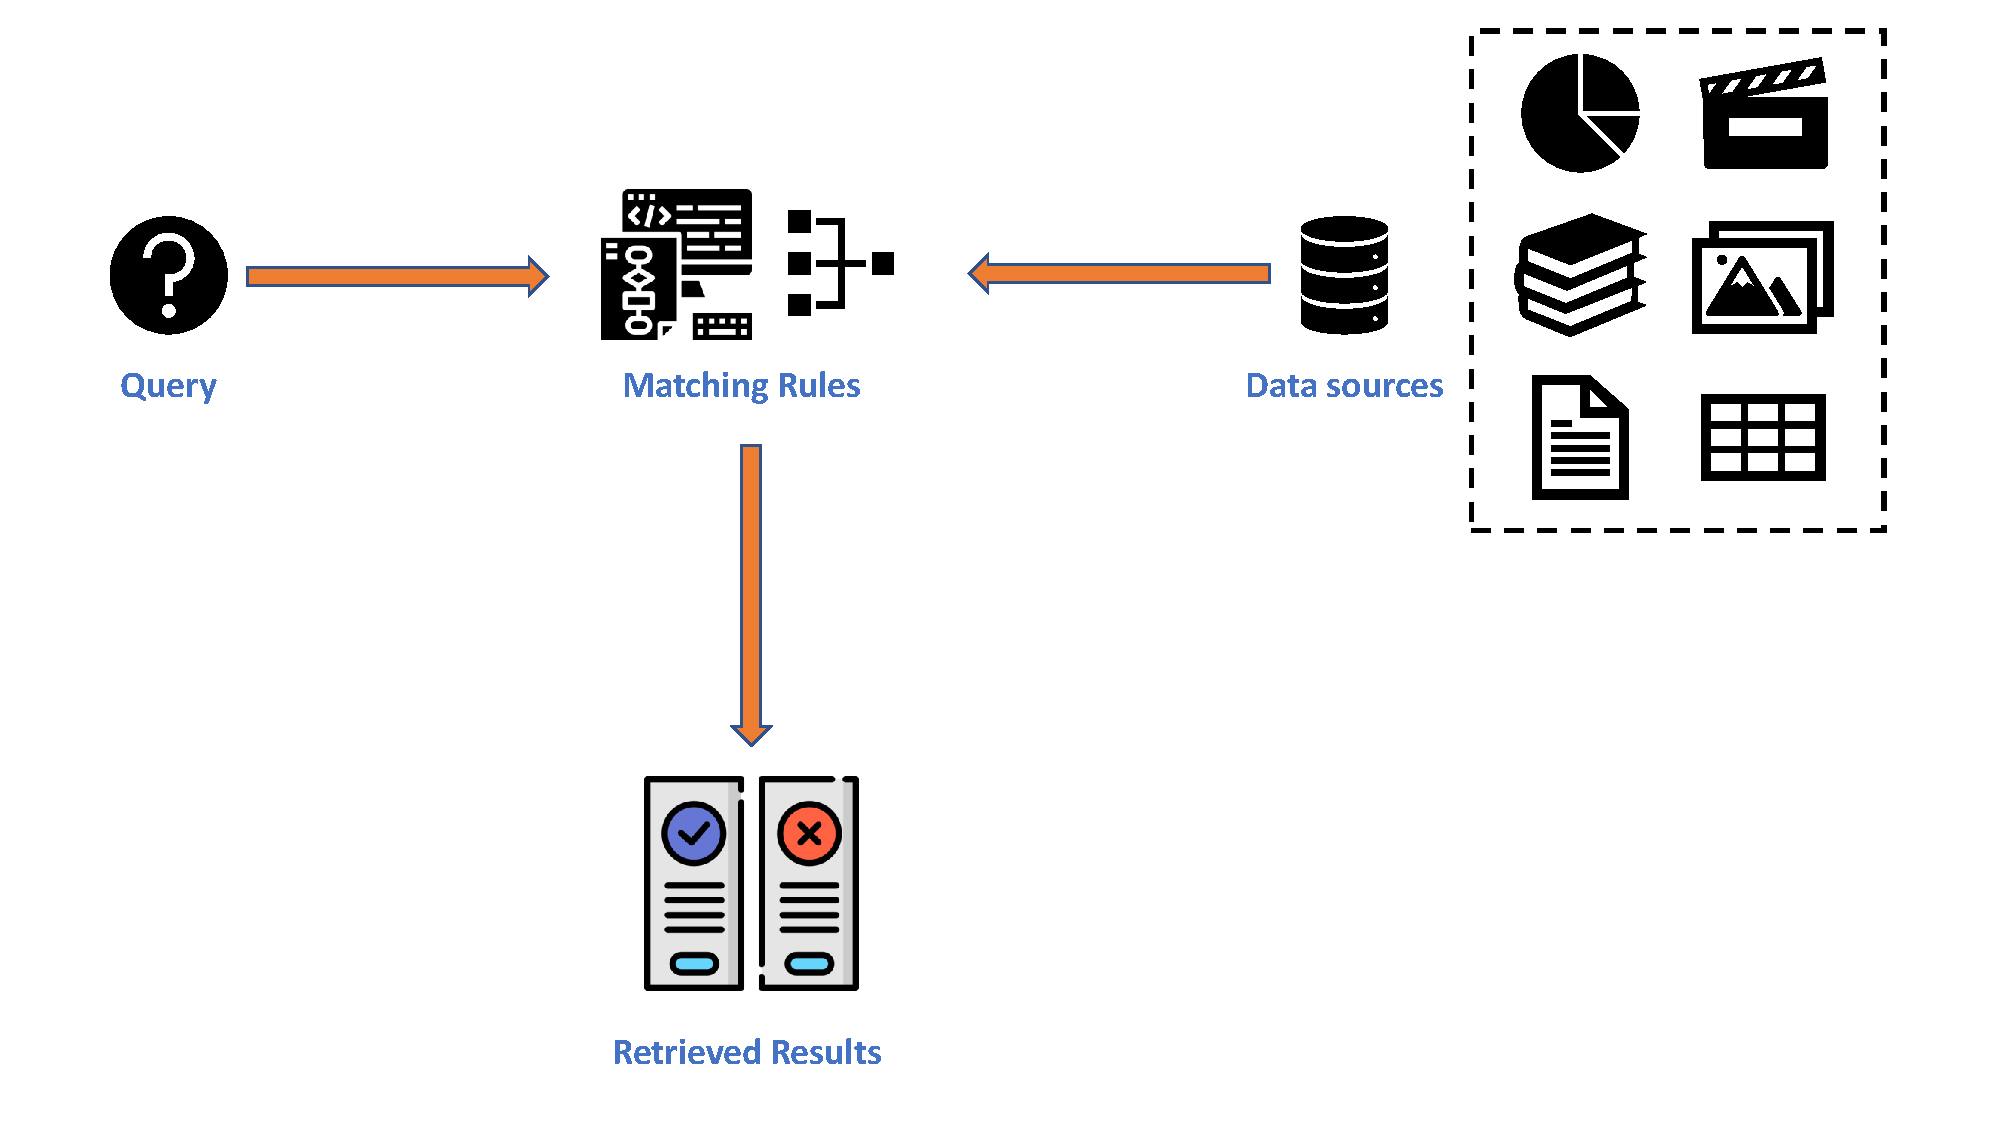
\includegraphics[width=\linewidth]{resources/images/overview/IR_structure.pdf}
    \caption{A simple overview of the Information Retrieval System}
    \label{fig:IR_structure}
\end{figure}
The need for such things occurred due to the increasingly rapid rise in data size and various kinds of information in different areas (like multimedia, website, scientific publication, etc.), making traditional searching techniques no longer cope.
In any IRS, there are always two aspects to deal with: system operation and matching algorithms. Since the first application in the 1940s, it has been developed continuously until now, with many essential milestones \cite{sanderson2012history} tackling both aspects.

%  paragraph 2
As the computing environment changes from time to time, many applications of IR have been suggested, like search on social networks, desktop element search, or one research hotspot recently named cross-modal retrieval.
This task aims to pick out relevant data across different modalities, such as image-text, video-text, audio-text.
Maragos et al. \cite{maragos2008multimodal} stated two future challenges with multimodal applications, including (i) Natural access and high-level interaction with multimedia databases and (ii) Detecting, recognizing and interpreting objects, events and human behavior in multimedia videos by processing combined audio-video-text data.
This statement also reflects two aspects that people always deal with the IRS, as mentioned above.
In research, people may care more about the method aspect than the other.
Traditional methods with manually designed representations, features and matching functions lack the ability to tackle complex IR tasks like multimodal interaction when those tasks require a deeper understanding of document contents and the user information needed \cite{culpepper2018research}.
However, thanks to an ever-stronger influence of Deep Learning \cite{goodfellow2016deep,lecun2015deep} in the 2010s decade, many problems raised in this field have resulted in better performance, letting people expect a new generation of robust and intelligent cross-modal Information Retrieval Systems.

%  paragraph 3
Also, humans have recently witnessed a rapid explosion in the appearance of videos in many aspects of their daily lives.
We all know the potential of videos in entertainment, communication, data analysis, etc.
The rise of video-based online services like YouTube, Netflix, along with the traditional TV program, has inspired Computer Vision (CV) experts to pay more attention to this resource. Additionally, natural language (NL) is one of the most effective means to describe those video contents.
From this point of view, the task of searching videos via text queries, or video-text retrieval, in short, becomes a desirable function in intelligent systems.
This problem takes (a) natural language text description(s) as input and outputs a sorted list of videos in terms of semantic relevance.
A lot of neuron network-based methods, focusing on transforming text input and video’s particular contents into the same subspace and measuring their similarity, have worked efficiently.
However, each video retrieval task has its own specificities among the diversity of the visual world, besides some in-tackling challenges like the semantic gap between two modalities, lack of annotated video-caption, or complicated consideration of temporal information, making no universal utilization approach fit for all such retrieval problems.
Therefore, caption-to-video retrieval is still attracting researchers to resolve in different areas.

\subsection{A brief introduction to Intelligent Transportation/Traffic System and the merits of Vehicle-oriented Computer Vision Tasks}
%  paragraph 1
Transportation is a non-separable part of any country, playing an essential role in different aspects of our daily life.
Residents, governments, and businesses almost depend on it to access resources.
Therefore, the advent of Intelligent Transportation/Traffic System (ITS), a significant factor contributing to the concept of smart city and to the development of modern civilization, is inevitable.
The implementation of ITS is widely accepted and used in many countries today when the governments recognize (i) the rapid growth of the human population, (ii) high-speed urbanization, and (iii) increasing vehicle ownership.
Though there are multiple modes of transportation, the roadway is the most common route.
So this kind of system aims to address a wide range of road traffic issues via advanced technologies, solving at three main levels: society, the road administrator, and drivers.
By providing different modules centering around the people-vehicle-road relation, and other traffic objects, it helps improve the safety, efficiency,  and environmental friendliness of the transportation.

%  paragraph 2
In an ITS that inherits Deep Learning works, Fan et al. \cite{fan2020deep} have shown that there are four major services in the architecture, as illustrated in figure \ref{fig:ITS_structure}.
\begin{figure}[!t]
    \centering
    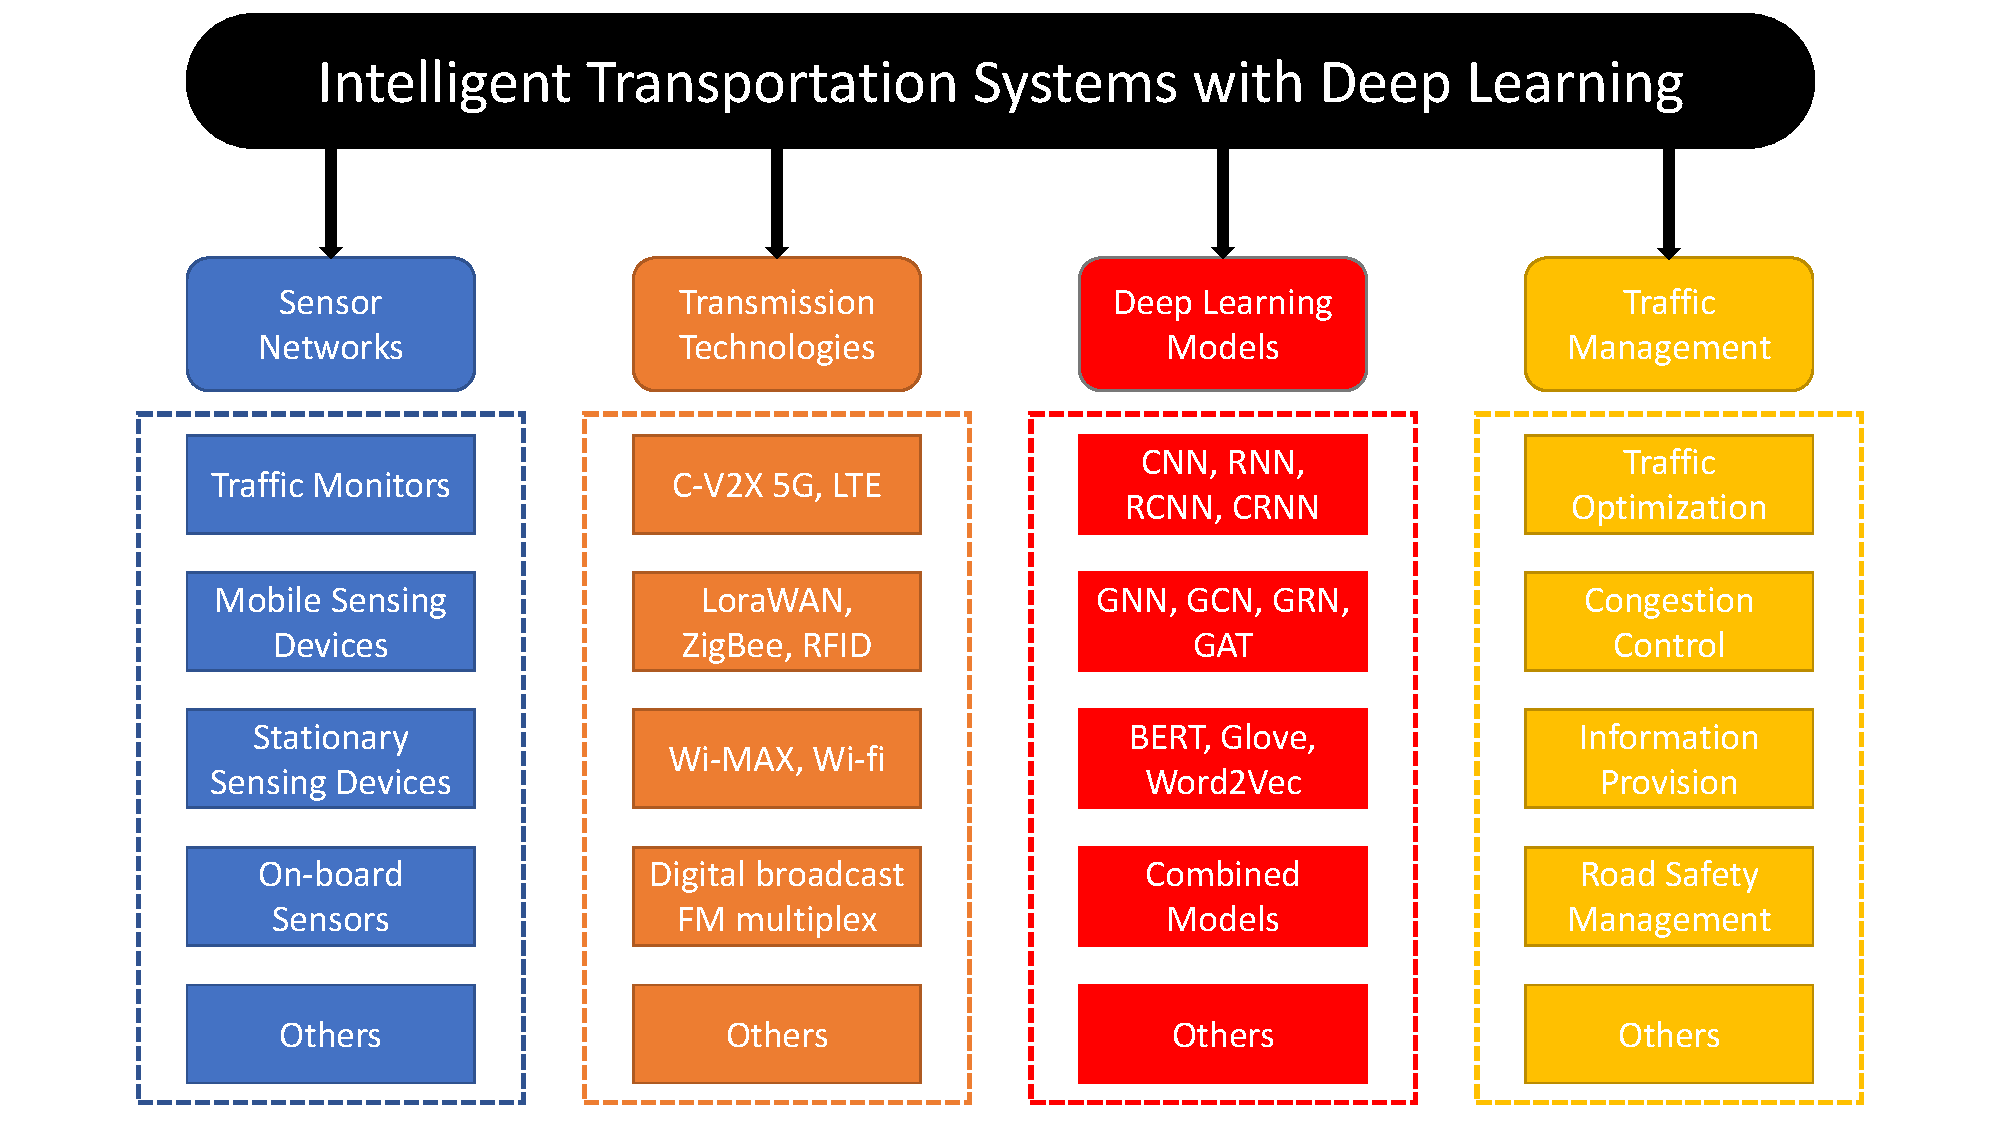
\includegraphics[width=\linewidth]{resources/images/overview/ITS_structure.pdf}
    \caption{Major components of a Deep Learning-based Intelligent Transportation/Traffic System.}
    \label{fig:ITS_structure}
\end{figure}
The Sensor Networks service is in charge of collecting real-time data then sends it through the Transmission Technologies service.
By exploiting the data, the Deep Learning Models service is responsible for building models that can perform well in particular tasks before integrating them into practical modules of the Traffic Management service.
When it comes to Computer Vision applications in such systems, many problems are mainly related to vehicles.
This is because transportation is vehicle-centered, unlike other areas, which are often people-focused.
Thanks to the widespread installment of 24/7 surveillance cameras on roads and highways, people can obtain massive traffic data.
Although the potential for video analytics from that data is enormous to be leveraged, it has not been exploited optimally.
Some tasks have received high-accurate state-of-the-art results, such as Vehicle Counting \cite{lu2021robust, dai2019video, asha2018vehicle} or Vehicle Reidentification \cite{luo2021empirical, Khorramshahi_2019_ICCV, zhu2019vehicle}, but some are still far from saturated outcomes.
Two major hurdles include the insufficiency of labels and the lack of high-performance models capable of converting data into valuable insights.
Regarding the model, since the vehicle is a particular domain and non-human, many pre-trained models cannot be applied directly to this object.
Therefore, CV researchers in this field still face so many significant challenges.
And, there should be something that can attract attention to address such issues.

%  paragraph 3
For those reasons, in parallel with the works of individuals, there are also organizations holding vehicle-oriented contests in order to find solutions from talented candidates.
Not stopping there, through these contests, people hope for deployments of submitted models into a realistic environment. 
One of the hottest contests is the AI City Challenge \cite{Naphade17AIC17, Naphade18AIC18, Naphade19AIC19, Naphade20AIC20, Naphade21AIC21}, opening continuously since 2017.
This contest primarily focuses on accurate, robust, and efficient approaches, so the organizers provide relatively sufficient labeled datasets \cite{Feng21CityFlowNL, Tang19CityFlow, Yao20VehicleX} as well as the evaluation system.
Their problems range from the mentioned tasks above to others like Velocity Estimation, Anomaly Detection, Vehicle Tracking, etc., whose insights may be inspired by various techniques.
In the latest edition, the 5th AI City Challenge \cite{Naphade21AIC21} has proposed a novel advanced track named Natural Language-Based Vehicle Retrieval (NL-based VR), which needs an effective combination of subtasks including motion detection, appearance recognition and content-based video retrieval.
There are still other tasks from other competitions, but finally, they all have the same goal: to solve real-world traffic issues and implement them into the Intelligent Transportation/Traffic System.
\section{Motivations}
\label{sec:motivation}
Segmentation is one of the problems where labels for models are scarce because of their high complexity and this cause a huge problem. Because if we cannot accurately label our data sets, then our models will never be as accurate as they could be. This is a real issue in the medical community, where human resources are often scarce. It's difficult to generate data when we have to prioritize human resources over machine labor. 

The supervised scenario is preferable to the unsupervised scenario in medical data because it is more accurate. The user has to manually annotate the pixel locations of interest with whole volume data. However, the problem occurs that for contiguous frames the difference is not much but the annotator has to time-consuming to perform the annotate action of similar positions on slices with not too different visual features. The unsupervised lack in the low-quality segmentation mask should be limited in terms of results and difficult to put into real life, especially for a field that requires absolute accuracy like medical.

The semi-supervised approach is a great way to take advantage of the benefits of both labeled and unlabeled data. By using this method, we can get more precise quantitative results based on the labeled data. This is important because it allows the model to exploit information from other raw data without any human guide. Additionally, the semi-supervised approach is able to do this while still maintaining accuracy in its results.

Nevertheless, in any scenario above, the process of manually labeling data is slow and inefficient. It can be difficult to reuse previous models, and the adaptability is low. This means that when labeling a new dataset, the process does not take advantage of the power of previous models. As a result, this slows down research and development in the medical field.

Video object segmentation is a pixel-level tracking object through sequence images problem. There are some similarities to when the expert user conducts labeling, although volume data is a 3-dimensional block, when performing labeling, the annotator has to go through each slice and make labeling, but cannot compare. Works conveniently with volume blocks. So now the volume becomes a sequence image and has many similarities with video object segmentation. Interactively volume object segmentation is a problem that has been proposed recently and has some promising directions for development, but it can be leveraged in the use of techniques that can be applied to problems encountered by medical data.

The points made above motivate us to investigate the potential of interactive segmentation with active learning. Such tools would work with people to find valuable positions for refinement and satisfaction of the result. With a certain number of slices, the tool could achieve results that are as good or even better than those produced by annotators.

\section{Objectives}
\label{sec:objectives}
\section{Thesis content}
\label{sec:thesis_content}

This thesis is structured into 7 chapters:

\textbf{Chapter 1}
In chapter 1, we present about the 3D CT volume organ segmentation task and its applications for many medical fields such as image-guided surgery, radiation therapy planning, and 3D printing. The purpose of this chapter is to provide an overview of the 3D CT volume organ segmentation problem and variants scenarios. We first discuss the problem statement and challenges involved in 3D CT volume organ segmentation. Next, we describe some key applications that can benefit from accurate 3D organ segments especially in interactive scenario. After that, we demonstrate our proposed approach overview for efficiency and accurately extracting organs from 3D CT volumes. Finally the thesis structure that we present will be overviewed.

\textbf{Chapter 2}
In chapter 2, we discuss all necessary background knowledge related to our work. First of all, we start with the very beginning concept in machine learning and then introduce some fundamental models used in processing complex data such as time-series or digital images. Then we introduce a list of Computer Vision problems which play an important role in our proposed approach. 

\textbf{Chapter 3}
In chapter 3, we introduce the volume organs segmentation problem, inspire from video object segmentation problem and is most related to our work. We also discuss the semi-supervised approaches which are widely used to solve medical image segmentation task and details about the state-of-the-art model that we utilized in our system. Next, we introduce related works which have a same scenario and motivation to solve the interactive segmentation concept. We provide detailed discussions about the Interactive methods and Positional encoding technique which applied directly to our propose architecture.

\textbf{Chapter 4}
In this chapter, we present our solution for tackle the interactive volume object segmentation. Our proposed approach include reference and propagation module. At first, the pipeline of the method is shown. Then, each module is introduced and the detailed implementation is presented. We apply the distillation technique not only in architecture design but also in the training strategy stage. Finally we dive deep in the potential of loss function especially for medical.

\textbf{Chapter 5}
In this chapter, we describe the experiment dataset, evaluation metrics, and challenge platform. Besides, we provide the details configurations and implementation details of our proposed method. Based on that, we also analyze the result with on our observations.

\textbf{Chapter 6}
In this chapter, we present the applications of our proposed method for interactive video volume segmentation, including a annotation tool. 

\textbf{Chapter 7}
In this chapter, we report the results and discuss about the future works for improving our proposed method and its applications. In our thesis, we proposed a novel pipeline to tackle the problem of CT volume organ segmentation along with an interactive tool that can help labeling process become less complicated. Overall, through ablation study, our method shows improvements over the original baseline, yet still have weaknesses. If these shortcomings can be resolved, we believe it can bring many breakthrough for both the deep leaning and medical fields. Having said that, it is left for the future works. 



% \chapter{Background}
\label{chap-background}
\begin{ChapAbstract}
In this chapter, we discuss all necessary background knowledge related to our work. First of all, we start with the very beginning concept in machine learning and then introduce some fundamental models used in processing complex data such as time-series or digital images. Then we introduce a list of Computer Vision problems which play an important role in our proposed approach. 
\end{ChapAbstract}


\section{CT Volume Image}
% ref https://www.ncbi.nlm.nih.gov/books/NBK574548/
CT images are two-dimensional pictures that represent three-dimensional physical objects. The images are made by converting electrical energy (moving electrons) into X-ray photons, passing the photons through an object, and then converting the measured photons back into electrons. The number of X-rays that pass through the object is inversely proportional to the density of the object. Objects imaged by CT consist of parts that vary in density. 

Image slices can either be displayed individually or stacked together by the computer to generate a 3D image of the patient that shows the skeleton, organs, and tissues as well as any abnormalities the physician is trying to identify. This method has many advantages make doctors easier to find the exact place where a problem may be located or identification of basic structures as well as possible tumors or abnormalities.

\subsection{Digital image representation}
% - how the computer store the images ?
In machine computing, image is a well-known definition. The image is construct by multiple pixels, each of them contains multiple values representing its visual information. The value range is often between from 0 to 255, for example it can handle the image brightness or the affect of a specific color (in a colored image). 
% insert image rgb 
Every image is define by structure information, such as image shape like channel, width, height. If the number of channel is 1, the image should be grayscale. And in color image, the number of channel would be 3 (corresponding with red, green and blue). And there are multiple variants of image type, like medical image shape would be constructed by width, height and depth. The depth channel could be thousand and pixel value range could be a negative number.
% insert volume image
\subsection{Hounsfield Units}
The CT detectors measure the degree that the scanned tissues physical density, and the image processor storing the data as pixels calculated by to convert byte data into a range of 5000 values. The scale's range of values is named for Hounsfield; each value on the scale is termed a Hounsfield unit (HU). Densities of various substances have been assigned relative values. The density of the substances in the patient (both natural tissues and any medical implants) and around the patient are calculated based on a linear transformation of the measured \textbf{X-ray attenuation coefficients}. This transformation is based on the standard density measurement of two substances, distilled water (set as 0 HU) and air (set as -1000 HU). HU for various scanned tissues are computed from the following equation: 
\begin{equation}
    HU = 1000 \times (tissue \mu - water \mu)/ water \mu 
\end{equation}
Where $\mu$ is the linear attenuation coefficient. CT scanners used in medical practice can present HU within a range of –1024 HU to +3071 HU. Different publications define different ranges for certain tissues and substances.

% Tissue physical density is proportional to photon attenuation (photon absorption). The CT detectors measure the degree that the scanned tissues attenuate photons (i.e., their density), and the image processor storing the data as bytes converts these values so that displayed pixels have proportionately assigned pixel brightness. A formula for this calculation to convert byte data into a range of 5000 values is used globally.[10][11] 

% The scale's range of values is named for Hounsfield; each value on the scale is termed a Hounsfield unit (HU). Densities of various substances have been assigned relative values, which are termed attenuation coefficients. The density of the substances in the patient (both natural tissues and any medical implants) and around the patient are calculated based on a linear transformation of the measured X-ray attenuation coefficients.[12] This transformation is based on the standard density measurement of two substances, distilled water (set as 0 HU) and air (set as -1000 HU) at 0 degrees Celsius temperature and a pressure of 10 Pascals.[13] HU for various scanned tissues are computed from the following equation: 

% HU =1000 X (tissue μ – water μ)/ water μ, where μ is the linear attenuation coefficient 
% CT scanners used in medical practice can present HU within a range of –1024 HU to +3071 HU.[14] Interpretation of clinical images often depends on evaluating a structure's HU, such as differentiating vascular lesions (which are dense when filled with contrast) from non-vascular lesions and distinguishing acute hemorrhage (which is dense) vs. non-acute hemorrhage or other substances. Different publications define different ranges for certain tissues and substances, for example: 


% \subsection{Image Windowing}

\section{Machine Learning and Deep Learning}
For the past decades, Machine Learning has become one of the most powerful tools, allowing individuals to perform complex analyses for better insights. The technique is widely applied and brings significant benefits in various vital fields, such as business, healthcare, agriculture or traffic management, etc.
Differ from the traditional programming paradigm, where the engineers have to craft the input data themselves and propose many rules to produce the most satisfying answers. \\
However, when the data increases extremely large, it contains many latent trends and patterns, which usually diminish hand-crafted solutions to get potential results.
This is where the Machine Learning techniques take place. The main goal of the approach is to develop a system that receives our observed data and corresponding expected answers, then return a set of rules that best fit those samples. These rules can be utilized to make predictions for new input. 
The machine-learning system applies some transformations on the input data to extract frequential or special patterns, which are usually called features, then use them to predict the output. The approach’s performance is then evaluated by appropriate metrics for the given task. Based on these scores, the system can choose the best transformation for each problem among a set of predefined functions (also known as hypothesis space). \\
As a subfield of machine learning, deep learning is formed as complex neural network architectures, containing more processing layers to learn hidden representations of the input data. 
This improvement is constructive in perceptual problems, where hand-crafted filters are merely impossible to achieve good results. 
In the following sections, we first discuss the beginning but original neural network to the further advanced ones.

\section{Deep Learning and Neural Network}
\label{model:mlp}

\subsection{Overview}
As a subfield of machine learning, deep learning is formed as complex neural network architectures, containing more processing layers to learn hidden representations of the input data. This improvement is constructive in perceptual problems, where hand-crafted filters are merely impossible to achieve good results. In the following sections, we discuss from the original neural network to the further advanced ones.

\subsection{Perceptron}

\begin{figure}[!h]
    \centering
    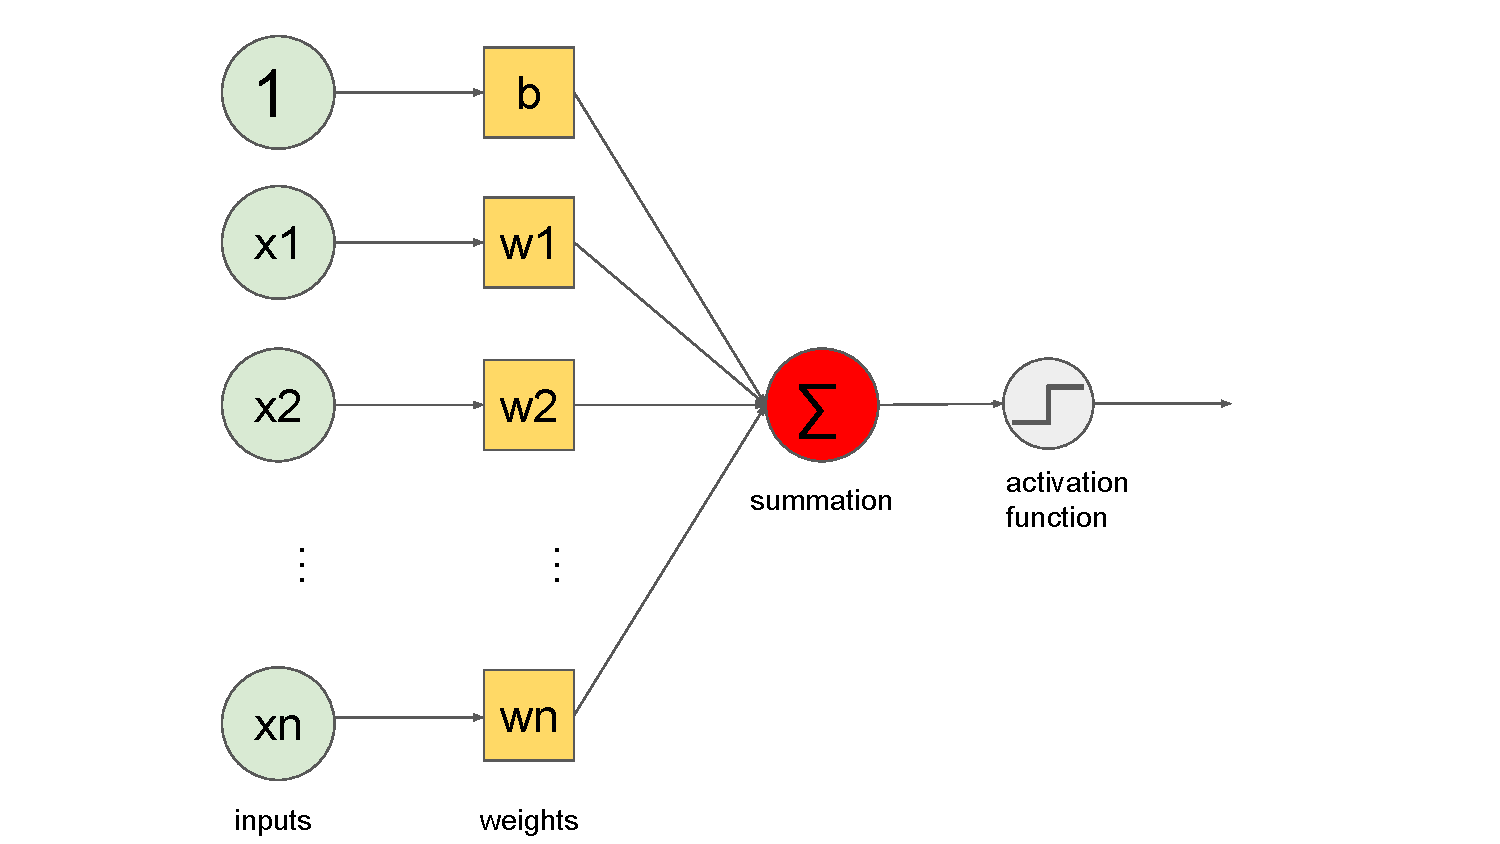
\includegraphics[width=\textwidth]{content/resources/new_images/related_works/perceptron.pdf}
    \caption{A single perceptron}
    \label{fig:perceptron}
\end{figure}

We first recap the early neural network, perceptron, which was introduced by Frank Rosenblatt in the 1950s \cite{rosenblatt1958perceptron} and 1960s \cite{rosenblatt1961principles}. 
The perceptron is an algorithm or a function for learning a binary classifier.
The function takes a $d$-dimensional vector $\mathbf{x}$ as input along with a weight vector $\mathbf{w}$ and calculates a single output value. 
\begin{align} \label{eqn: perceptron}
    a = f(\mathbf{x}) = \sigma(\mathbf{w}^T\mathbf{x} + b)
\end{align}
where $\mathbf{w}^T\mathbf{x} = \sum_{i=0}^{d} \omega_{i}x_{i} $ denotes the inner product between the input and weight vector and $b$ is bias. The perceptron behaves as a nonlinear function $\sigma$ of a linear combination of the input where each element $x_{i}$ is multiplied with it's corresponding coefficient $\omega_{i}$. 
Figure \ref{fig:perceptron} illustrates the process of a single perceptron process.\\
At first, the perceptron function is designed to solve the \textit{binary classification} problem in which each datapoint $\mathbf{x}$ belongs to a single class (denoted as \textbf{1} or \textbf{0}) and the weight vector $\mathbf{w}$ represents a boundary hyperplane that splits the space into two classes seperately. 
Therefore, points that lie at the same side of the plane are grouped to the same class. 
And the $sign$ function is used as activation function $\sigma$ in \ref{eqn: perceptron} to return $1$ if the combination is positive and $0$ otherwise.
\begin{align} \label{eqn: sgn_perceptron}
    a = f(\mathbf{x}) = \left\{\begin{matrix}
1 & \text{\quad if \quad} \mathbf{w}^T\mathbf{x} + b\geq 0 \\ 
0 & \text{\quad if \quad} \mathbf{w}^T\mathbf{x} + b <  0 
\end{matrix}\right.
\end{align}

\subsection{Activation functions}

Different from perceptron, activation function here is continuous, which makes the network weights differentiable with respect to output signals. \\
\begin{figure}[h]
    \centering
    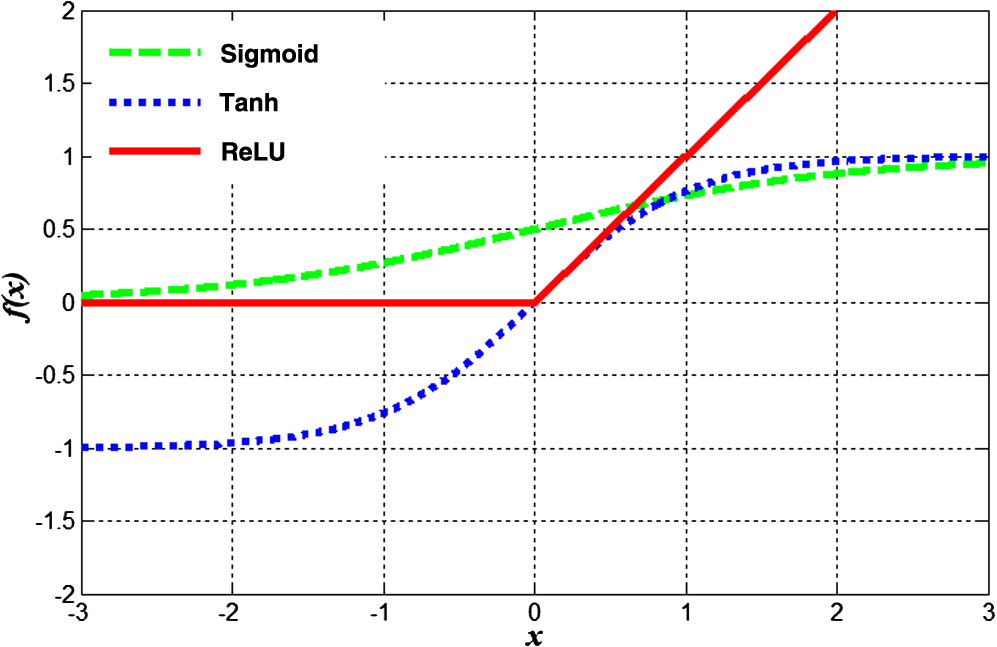
\includegraphics[width=0.7\textwidth]{resources/images/activation.png}
    \caption{Plot of Sigmoid, Tanh and ReLU activation functions.}
    \label{fig:activation}
\end{figure}
Here we list some of those activation functions commonly used in neural network modeling:
\begin{align} \label{eqn:sigmoid}
    \mathrm{sigmoid}(x) = \frac{1}{1 + \exp(-x)}
\end{align}
\begin{align} \label{eqn:tanh}
    \mathrm{tanh}(x) = \frac{\exp(2x - 1)}{\exp(2x + 1)} = 2 \times \mathrm{sigmoid}(2x) - 1
\end{align}
\begin{align} \label{eqn:relu}
    \mathrm{relu}(x) = \mathrm{max}(0, x)
\end{align}
The $sigmoid$ function (\ref{eqn:sigmoid}) scales real numbers to the range $[0, 1]$, where the large positive numbers change to $1$ and the large negative ones become $0$. Similar to $sigmoid$ but aims to produce zero-centered signals, $tanh$ function (\ref{eqn:tanh}) is a scaled version of $sigmoid$ with values range of $[-1, 1]$.\\
The drawback of both $sigmoid$ and $tanh$ is that when the numbers are large, the squashed values are saturated, hence their gradients is extremely small, which leads to the vanish problem when training deep neural networks. In such cases, Rectified Linear Unit ($ReLU$, \ref{eqn:relu}) is preferably used, which converts negative values to zero while keep the positive ones.
Figure \ref{fig:activation} illustrates the three functions in the same input range.



\subsection{Artificial Neural Networks}

The study of artificial neural networks (ANNs) has been inspired by the observation that biological learning systems are built of very complex webs of interconnected neurons in brains. The human brain contains a densely interconnected network of approximately trillion of neurons. ANN systems are motivated to capture this kind of highly parallel computation based on distributed representations. 

Generally, ANNs is a combination of a large number of interconnected processing neuron organized in a multi-layer architecture, where signal from a neuron can be passed to another from nearby layers (figure \ref{fig:neural_nets}). Each neuron is also formulated the same form as \ref{eqn: perceptron}. In general, neural network has an input layer, an output layer and a predefined number of hidden layers. Each hidden layer stands for a single transformation step in the process, which aims to extract hidden patterns of the input stored in it's neurons.  In recent years, state-of-the-art neural networks have multiple hidden layers. The number of layers determines the depth of the network, in contrast to the width of the network, which is determined by the maximum number of neurons between the hidden layers. In many cases, increasing depth increases the complexity of
the model, creates more space to store information and therefore increase its learning capability. These information is continually passed to following layers to extract more essential features. Due to the fact that sequence of linear transformations always equals to a single linear one, neural network uses nonlinear activation function $\sigma$ to element-wise apply to each processed neuron. 

\begin{figure}[h]
    \centering
    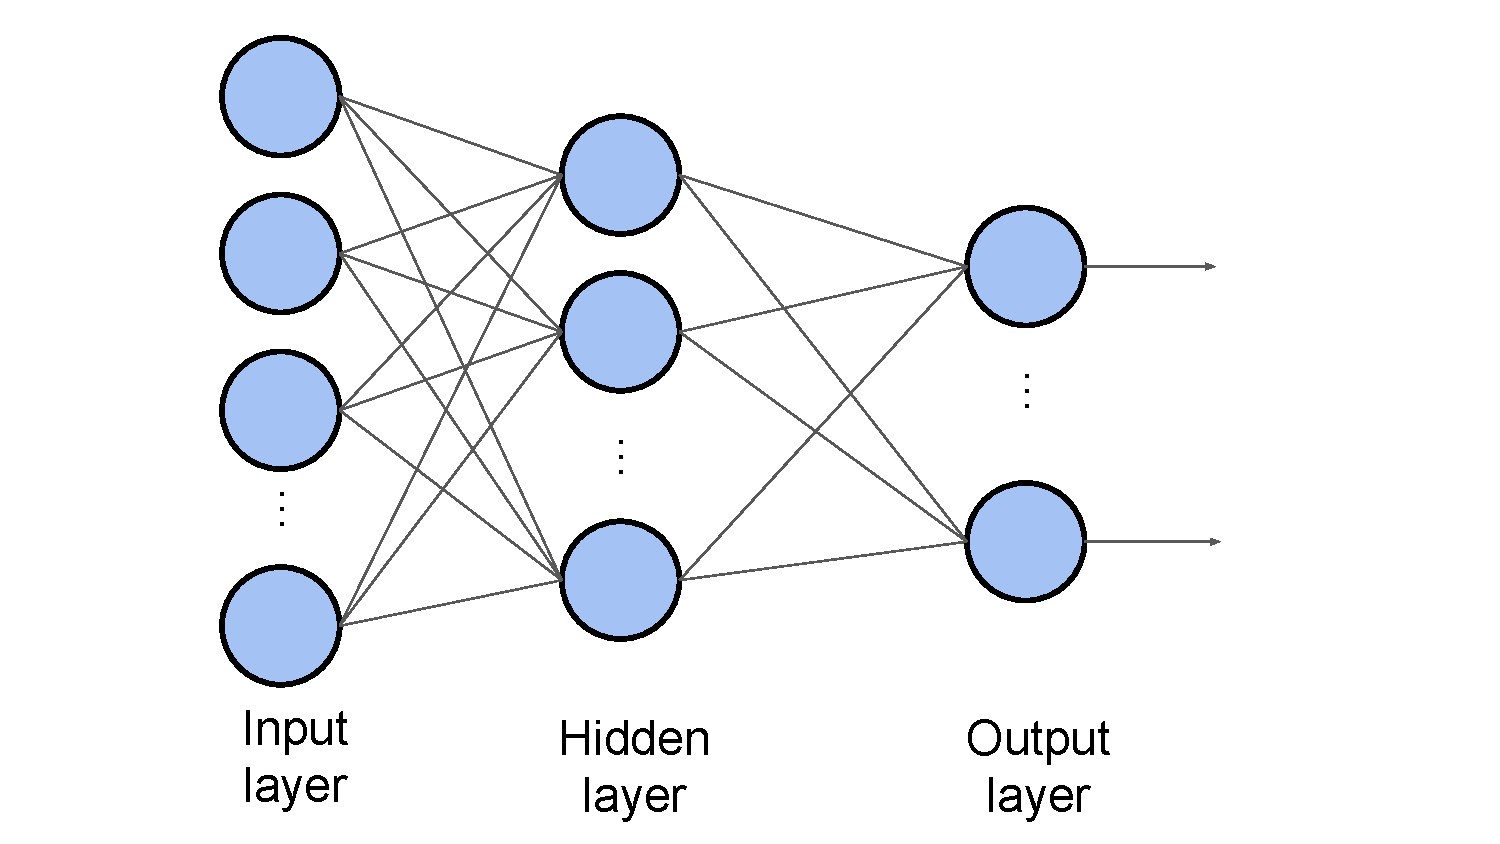
\includegraphics[width=0.7\textwidth]{content/resources/new_images/related_works/neural_nets.pdf}
    \caption{A simple three-layer neural network}
    \label{fig:neural_nets}
\end{figure}


Researchers have been actively conducting research on designing the architecture for ANNs to tackle machine learning and deep learning problem. Each new network design establishes on top of the older ones and each aims to solve a specific task independently. In order for the networks to deal with different tasks, such as classification, object detection, human action recognition, it cannot be without the usage of loss functions.

\subsection{Loss functions}

As stated in \ref{sec:ml}, supervised-learning neural networks must be trained with plenty of inputs-outputs data pairs. With every input, the network is expected to give a predictive outcome. While training, the network continuously adjusts its weights to minimize the discrepancy between its predicted outcome and the real outcome. The value of the discrepancy is often measured by using loss functions.

Loss functions are very diverse, each aims to solve different things and also is used for different tasks. For instance, in the regression task, the most used loss function is the least mean squared error. Suppose we have a model with parameters $\theta$, given a training sample $(x,y)$ where $x$ is the input and $y$ is the ground-truth, the loss for this single sample is calculated as follows

\begin{equation}
    \mathcal{L}(\theta,x,y) = \frac{1}{2} [y - h_{\theta}(x)]^2
\end{equation}

Similarly with classification task, the most frequently used one is cross-entropy loss. With the same notation as the example above, the loss function is as follows

\begin{equation}
    \mathcal{L}(\theta,x,y) = - (1-y_i) \text{log}(1-h_\theta(x_i)) - y_i\text{log}h_\theta(x_i)
\end{equation}

There are various factors involved in choosing a loss function for specific problem such as type of machine learning algorithm chosen, ease of calculating the derivatives and to some degree the percentage of outliers in the data set. 

So far, loss functions are used to determine the error between the output of our algorithms and the given target value. For the networks to perform better, it is essential to minimize the loss value. For only one training sample to be minimized, it is undoubtedly easy.
However, in practice, the loss value should be estimated for every possible training samples; this is nearly impossible. Therefore, the process of training can be formulated as an optimization problem: 

\begin{align}
    \mathcal{J}(\theta) &= E_{x,y} [L(\theta, x, y)] \approx \frac{1}{n} \sum^n_{i=1} L(\theta, x_i, y_i)
\end{align}

where $(x_i, y_i)$ is the $i^{th}$ oair and $n$ is the number of pairs in the dataset.
The target is to search for a set of parameters $\theta$ which minimize the expected loss function, or more realistically, calculate its approximation. An effective algorithm for this task is gradient descent, which is a fundamental tool of modern machine learning problems.

\subsection{Gradient descent}

Gradient descent (GD) is an iterative optimization algorithm used to find the local minimum of an objective function $J(\theta)$ by updating the parameters $\theta$ in the opposite direction of the gradient of that objective function. A gradient simply measures the change in all weights with regard to the change in error. In mathematical terms, a gradient is a partial derivative with respect to its inputs. 

How big the steps the GD takes into the direction of the local minimum are determined by the learning rate $\alpha$, which figures out how fast or slow we will move towards the optimal weights (as illustrated in Figure \ref{fig:gradient_descent}). Small value of $\alpha$ might lead to consistency but slow progress while larger one can result in faster progress but risk divergence. Thus, it must be carefully chosen. 

\begin{figure}[h]
    \centering
    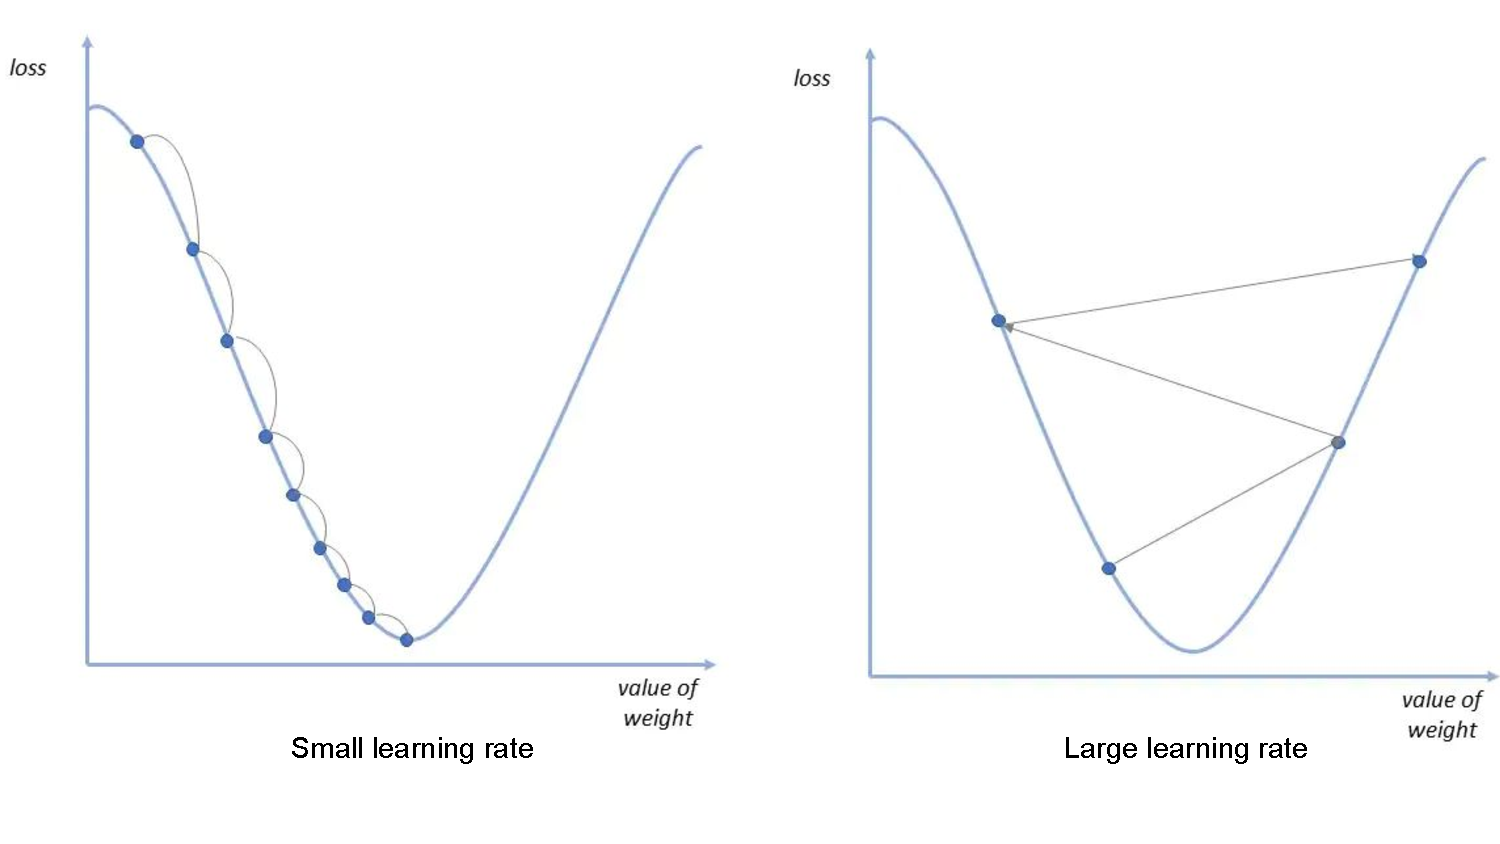
\includegraphics[width=0.9\textwidth]{content/resources/new_images/related_works/gradient_descent.pdf}
    \caption{Gradient descent}
    \label{fig:gradient_descent}
\end{figure}
 

Mathematically, the parameter $\theta_i$ in the set of parameters $\theta$ is updated as follows:

\begin{align}
    \theta_i := \theta_i - \alpha \frac{\partial J(\theta)}{\partial \theta_i}
\end{align}

While the original GD, also called vanilla GD, performs weights update after one pass through the whole dataset, which can be costly in practical scenario, there has been various variations that can alleviate this problem.
Stochastic gradient descent (SGD) \cite{bottou2010large} updates the parameters for each calculated training example one by one, which can help faster convergence than vanilla GD depending on the problem.  Additionally, the frequency of those updates can result in noisy gradients, which may cause the error rate to fluctuate instead of slowly decreasing. For the most strategic method, it must be the Mini-batch GD variant. It simply splits the training dataset into small batches and performs an update for each of those batches. From this variant, others with more parameters and mechanisms beside learning rate are introduced to improve the consistency and convergence speed of the algorithm, such as Adam \cite{kingma2014adam} or RMSProp.


\subsection{Feed-forward and Back-propagation}

\textbf{Feed-forward} describes the process of information flowing forward through the entire neural network. Given input data $x$, it is propagated through the intermediate layers to finally produce $\hat{y}$ at the output layer. Feed-forward is used both in the training and the testing phase to make predictions for any given input. In the training stage, the error is estimated between the network's output and ground truth; that essentially provides gradient information to update the network parameters. 

\textbf{Back-propagation} 
With the loss computed, back-propagation computes the gradient with respect to the weights of the network for a single input-output pair, and then flow the gradient information backward through the network . At each of the layers, new gradients are computed based on the following layers by the chain rule, then it is used to update the parameters in these layers using gradient descent. The process happens again until the gradients at the input layer are calculated and updated.

The process of feed-forward and back-propagation keep on repeating, and the weights keep updating continuously until the network becomes better fitted to the data that was fed into it, with reasonable evaluation result.

\section{Convolutional Neural Network}
\label{model:cnn}
Convolutional Neural Network (CNN or ConvNet) is a special case of fully-connected neural network discussed in previous session, which was specially designed to process grid-like topology data, such as images.
For example, with an image of size $[32, 32, 3]$, a single unit at first hidden layer in fully-connected neural network would have $32 \times 32 \times 3 = 3072$ weights corresponding to all the pixels. 
This amount increases exponentially with image size, the $[224, 224, 3]$ image would cost over $150000$ weights for each neuron. 
This make the network cost a lot of computation and easily overfit.
Furthermore, the traditional neural network views each image as a flatten vector, which may lead to lack of spatial information, given by groups of nearby pixels. Take inspiration from the biological visual system, each neuron in CNN only look at a restricted region (known as \textit{receptive field}) of the input image. \\
\begin{figure}[t!]
    \centering
    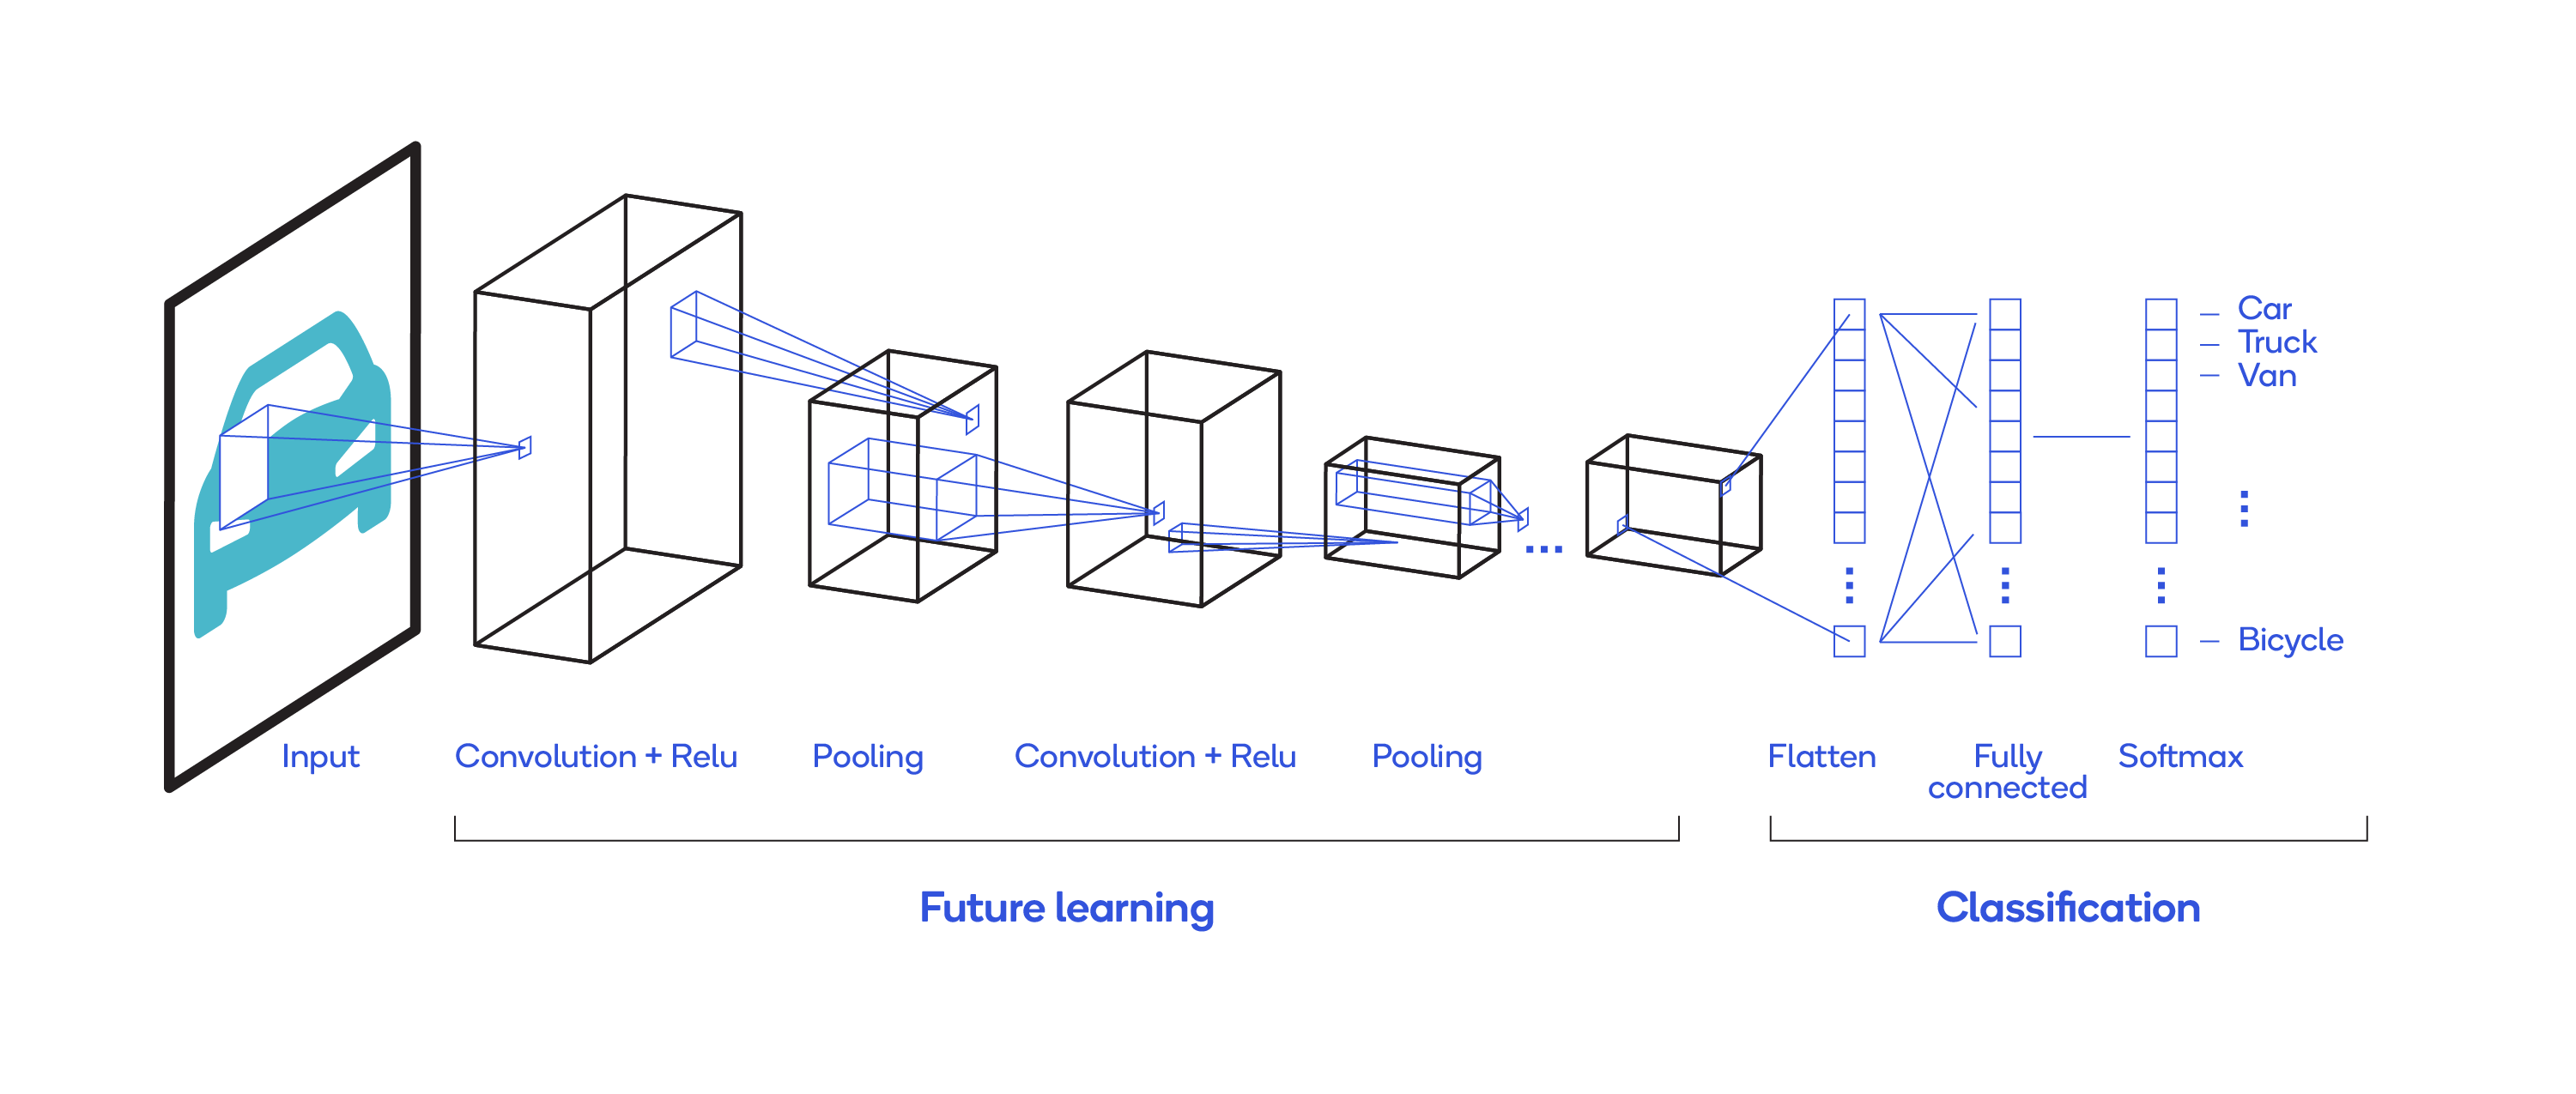
\includegraphics[width=\textwidth]{images/CNN.png}
    \caption{A neural network architecture for image classification task, constructed from convolutional layer, pooling layer and fully-connected layer.}
    \label{fig:cnn}
\end{figure}
Concretely, a simple ConvNet is constructed from a sequence of individual layers (illustrated in figure \ref{fig:cnn}): \\
\textbf{Convolutional Layer}. \quad The most important component in a CNN architecture. Receive an input volume from previous layer, the layer apply a convolution function using an adaptive \textit{kernel} (or \textit{filter}) to compute outcome neurons for current layer. The operation works as sliding the \textit{kernel} across the entire input then compute dot product between the covered input values and the filter entries. An activation function is also applied on each neuron value, as mentioned in \ref{model:mlp}. By this function, we output a 2D feature map with the shape usually smaller than the input volume. Intuitively, the convolution works as a pattern identifier, aims to extract visual feature given in images such as object edges or other special shapes, etc. \\
Some important hyper-parameters used to define a convolutional layer:
\begin{itemize}
    \item Kernel size: $[K \times K \times C_{in}]$, predefined shape of filter matrix used in convolution process. $C_{in}$ is the input channel of input tensor from previous layer.
    \item Number of kernel: $N_{k}$, the amount of kernels we apply at the current layer. Each kernel correspondents to a specific convolution layer, used to produce a 2D feature map. Finally, we stack these maps to achieve the output volume.
    \item Stride: $S$, the number of pixels that the kernel splits on the tensor.
    \item Padding: $P$, the number of rows/columns used to pad the input around the border. This step helps to reduce the information loss as the border pixels are not used as frequently as the inner ones.    
\end{itemize}
\textbf{Pooling Layer}. \quad The layer used to reduce the spatial size of the output feature map produced by successive convolutional layer. This technique helps to reduce computation cost and amount of parameters, and hence, help to control overfitting. \\
\textbf{Fully-Connected Layer}. \quad The layer performs exactly as a Neural Network mentioned in section \ref{model:mlp}. Receive the final representation from previous step, fully-connected layer provides a stack of dense connection to get the final prediction for a specific task. For example in image classification problem, the layer produce an output vector $\mathbf{o} \in \mathbb{R}^{c}$ ($c$ is the number of target classes), then apply a softmax function to give prediction confidence. \\
% Figure ... shows an example of a typical CNN architecture.\\
In general, ConvNet can be seen as a two-stage process, feature learning and prediction. The feature learning stage built from stack of convolution-pooling blocks, aims to produce the final representation of the input image while the prediction stage utilizes this embedded information for a specific tasks.
Therefore, the ConvNet is also commonly used for feature extraction and can be efficiently applied in various tasks such as Image/Video Retrieval, Instance Re-identification or Image Generation, etc. 

% \subsection{Modern convolutional networks}
% In this section, we 
% [TODO]
\section{Transformer}
\label{sec:transformer}
“Attention is All you Need” (Vaswani, et al., 2017) \cite{vaswani2017attention}, is impactful work in both natural language processing or computer vision field. It presented a lot of improvements and the proposed “transformer” model is entirely built on the self-attention mechanisms without using sequence-aligned recurrent architecture (which will describe in section \ref{subsec:attention}). The Transformer model has an encoder-decoder architecture, as commonly used in many natural machine translation models. Later decoder-only Transformer was shown to achieve great performance in language modeling tasks, like in GPT and BERT. Nowadays, transformer also use in computer vision because of the context-understanding ability of it and become one of the state-of-the-art.

\subsection{Sequence to sequence (Seq2Seq)}
The seq2seq model was introduced by Sutskever \cite{sutskever2014sequence}, et al in the language modeling field. It tackle the transformation of an source sequence to a target one, firsly apply in neural machine translation (figure \ref{fig:seq2seq}). The seq2seq model normally has an encoder-decoder architecture, composed of:

\begin{itemize}
    \item \textbf{Encoder}: to compress the information of input sequence and represent it as an context vector. This representation is expected to be summery the whole source sequence.
    \item \textbf{Decoder}: is initialized with the context vector to emit the transformed output. Seq2seq only used the last embedding state of the encoder network as the decoder initial input.
\end{itemize}
\begin{figure}
    \centering
    \includegraphics{}
    \caption{The sequence to sequence overview}
    \label{fig:seq2seq}
\end{figure}
This architecture is the foundation of many sequential models nowadays, but still exist few limitations such as use a fixed-length context vector. And one of the the most improvements handle this problem is attention mechanism.

\subsection{Attention and Self-Attention mechanism}
\label{subsec:attention}
\textbf{The attention mechanism} uses to memorize long source sentences in neural machine translation. Define the attention mechanism in a scientific way. Say, we have source sequence \mathbf{x} have length $n$ and target sequence \mathbf{y} have length $m$
\begin{equation}
\mathbf{x} &= [x_1, x_2, \dots, x_n] \text{;}
\mathbf{y} &= [y_1, y_2, \dots, y_m]
\end{equation}

The key idea is it create weighted shortcuts between the context vector and the entire source input. The alignment between the source and target is learned by a context vector. The context vector is a sum of hidden states $\boldsymbol{h}_i$ of the encoder sequence and weighted by alignment scores $\alpha_{t,i}$, in there $\alpha_{t_i}$ is calculate from the hidden states $\boldsymbol{s}_i$ from the decoder. 

\begin{equation}
\label{eq:align_score}
\mathbf{c}_t &= \sum_{i=1}^n \alpha_{t,i} \boldsymbol{h}_i & \small{\text{; Where $c_t$ is the context vector for output }y_t}
\end{equation}

The alignment score $\alpha_{t,i}$ is assign by a model to the pair of input at position and output at position based on how well they match. The set of pairs are weights how much of each source hidden state should be considered for each output. The score function is therefore in the following form below at timestamp $t$:
\begin{equation}
    e_{ij}=a(s_i,h_j), \qquad \alpha_{i,j}=\frac{\exp(e_{ij})}{\sum_k\exp(e_{ik})}
\end{equation}

\textbf{Self-attention} is an attention mechanism variant, in that it relating different positions of a single sequence in order to compute a representation of the same sequence. The self-attention mechanism use to learn the correlation between the current token and the previous part of the sequence. 

\subsection{Multi-head Self-Attention}
In the paper attention is all you need, transformer component have re-define the attention by using retrieval concept. The encoded representation of the input as a set of key-value pairs $\mathbf{K}, \mathbf{V}$.
In the decoder, the previous output is compressed into a query $\mathbf{Q}$ and the next output is produced by mapping this query and the set of keys and values.  

\begin{equation}
    \text{Attention}(\mathbf{Q}, \mathbf{K}, \mathbf{V}) = \text{softmax}(\frac{\mathbf{Q}\mathbf{K}^\top}{\sqrt{n}})\mathbf{V}
\end{equation}
Where $n$ is the dimension of the source hidden state. And we have a scalar score $a_{ij}$ follow
\begin{equation}
    a_{ij} = \text{softmax}(\frac{\mathbf{q}_i {\mathbf{k}_j}^\top}{\sqrt{n}})
= \frac{\exp(\mathbf{q}_i {\mathbf{k}_j}^\top)}{ \sqrt{n} \sum_{r \in S_i} \exp(\mathbf{q}_i {\mathbf{k}_r}^\top) }
\end{equation}
The reason behind this because the attention operation can be thought of as a retrieval process as well. As mention in eq \ref{eq:align_score}, if we remove the constraint that the weight $\alpha_{t}$ is a one-hot vector, the operation could be thought as a retrieval process according to the $\alpha_{t}$ as a probability vector. This way efficiency computes the vector $\alpha_{t}$ as a matrix multiply to measure the similarity by project $s$ and $h$ to a common space instead of we have to go through the network $n \times m$ times to acquire all the attention scores $a_{ij}$.
\begin{equation}
    \label{eq:scale_dot_product}
    \text{score}(\boldsymbol{s}_t, \boldsymbol{h}_i) = \frac{\boldsymbol{s}_t^\top\boldsymbol{h}_i}{\sqrt{n}}
    \caption{Scaled dot-product formula}
\end{equation}
\textbf{The multi-head self-attention module} is a key component in transformer. In summary, the idea of multi-head attention is to split the feature dimension of the input into many parts and attention over these sub-dimensions. Then computes the scaled dot-product attention (eq \ref{eq:scale_dot_product}) over each subspace in parallel. Each independent attention outputs are simply concatenated and linearly transformed into expected dimensions.
\begin{figure}[h]
    \centering
    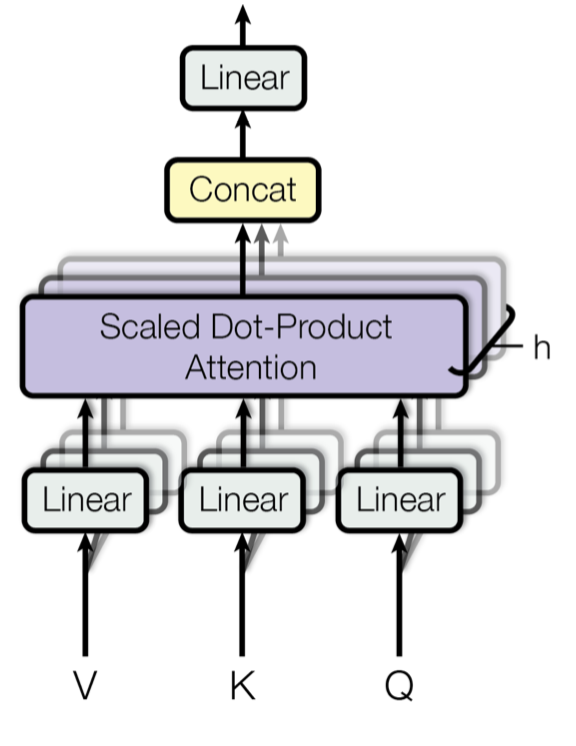
\includegraphics[height=2in]{content/resources/new_images/background/multi-head-attention.png}
    \caption{Multi-head scaled dot-product attention mechanism \cite{vaswani2017attention}}
    \label{fig:multiheadatt}
\end{figure}
\subsection{Transformer architecture}

\begin{figure}[h]
    \centering
    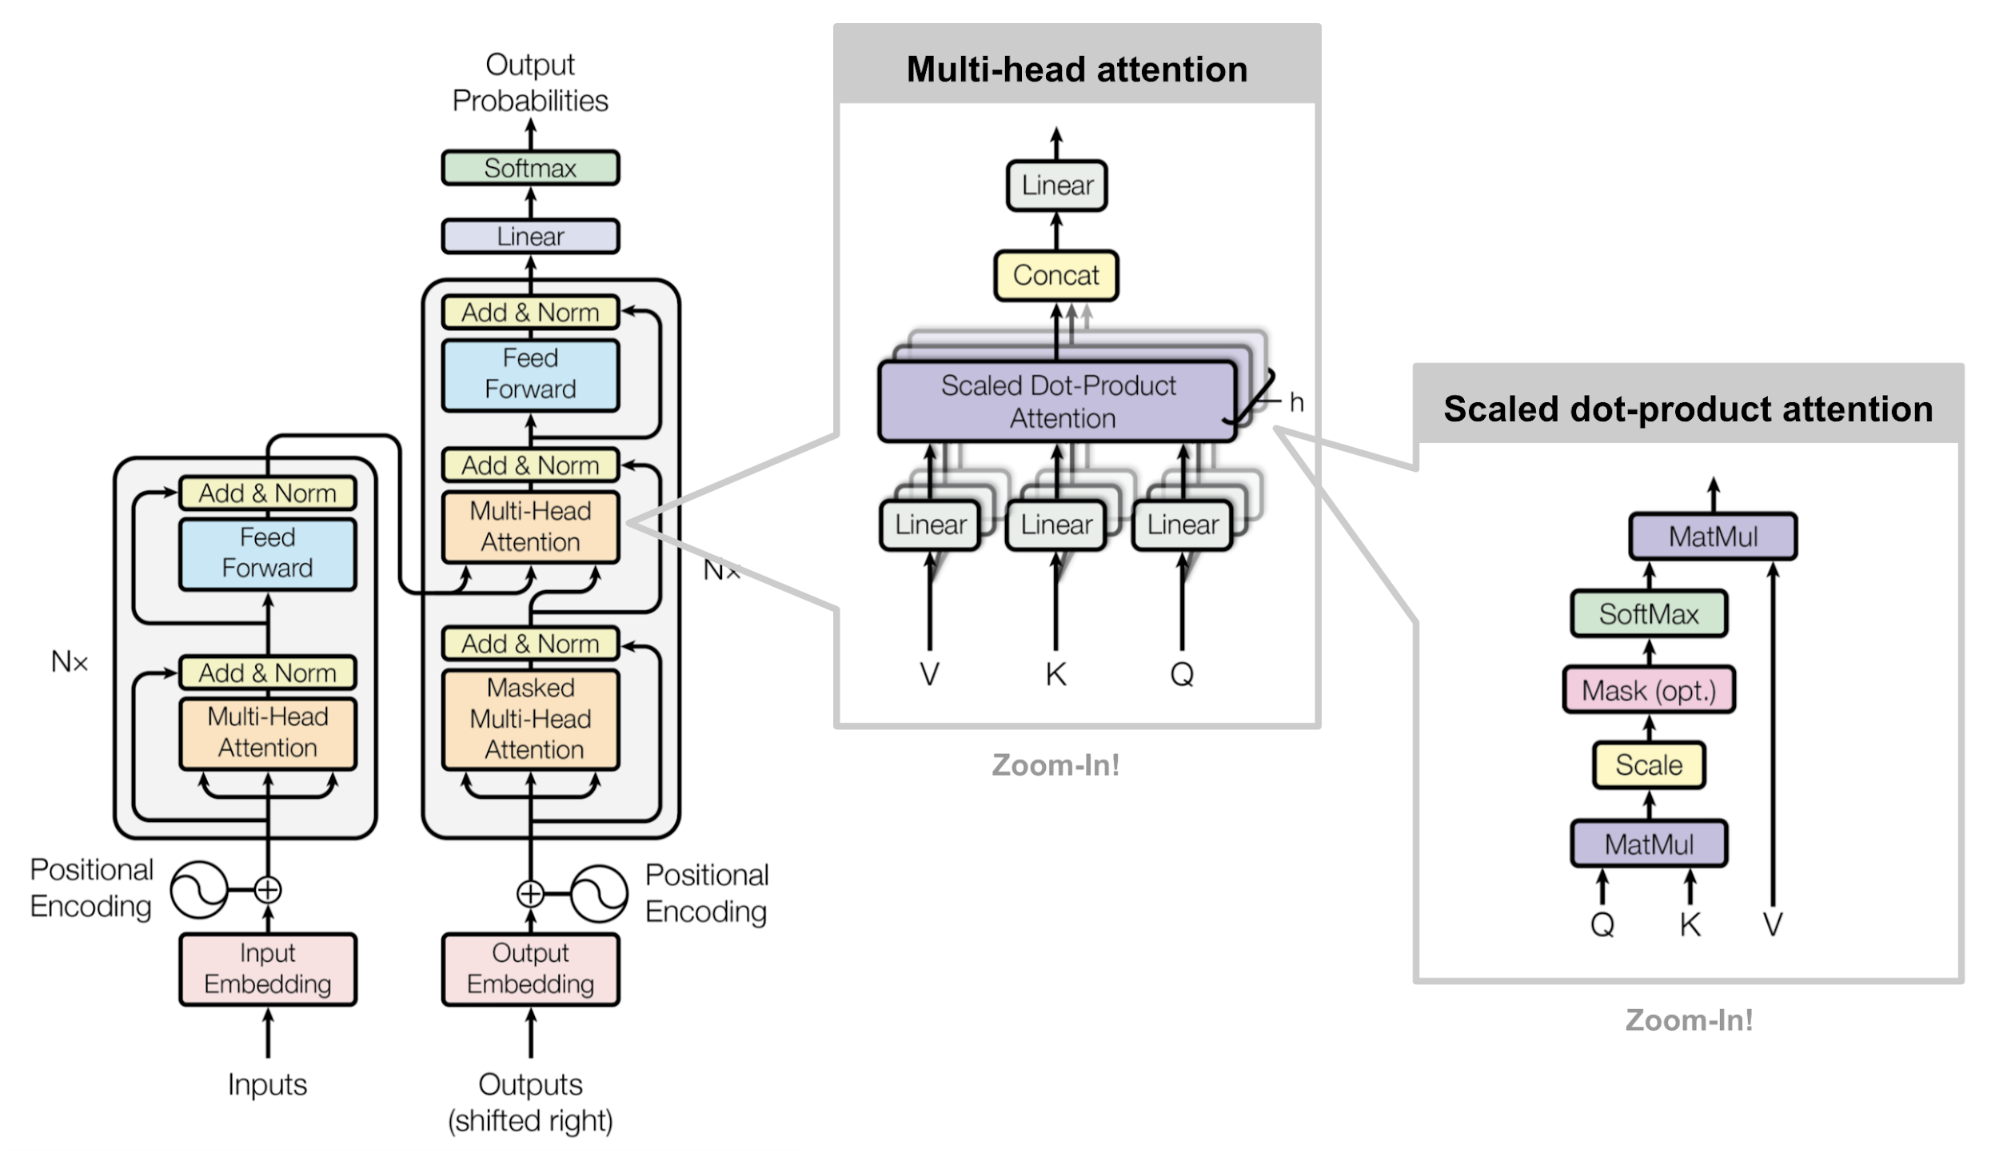
\includegraphics[width=\textwidth]{content/resources/new_images/background/transformer.png}
    \caption{The full transformer architecture \cite{vaswani2017attention}}
    \label{fig:transformer_arch}
\end{figure}


Transformer model has an encoder-decoder architecture. The encoder generates a representation from a large context. It constructed by two main submodules, a \textit{multi-head self-attention} layer and a \textit{projection network}. 

In the transformer decoder is retrieve information from the encoded representation. The architecture is quite similar to the encoder. Figure \ref{fig:transformer_arch} shown the whole propose architecture




% \chapter{Related Works}
\label{chap-related-works}
\begin{ChapAbstract}
In this chapter, introduce the volume organs segmentation problem, inspire from video object segmentation problem and is most related to our work. We also discuss the semi-supervised approaches which are widely used to solve medical image segmentation task and details about the state-of-the-art model that we utilized in our system in section \ref{sec:segmentation} and \ref{sec:semisup} 
Next, we introduce related works which have a same scenario and motivation to solve the interactive segmentation concept. We provide detailed discussions about the Interactive methods and Positional encoding technique which applied directly to our propose architecture in section \ref{sec:mask_propagate} and section \ref{sec:positional_encoding}).
\end{ChapAbstract}
% \section{Video-text retrieval}
\label{sec:video-text_ret}
Representation Learning (RL) aims to learn compact features of high-dimensonal data (e.g. image, video, audio or document), which has a range of applications in cross-modal context matching. Especially between visual and textual information, it learns to embed the vision and language information into the same latent space, where similarities of different modal features reflect the proximity of their original semantics. \\
The image-text matching task is related to various problems such as Image Captioning (\cite{vinyals2015show, xu2015show, anderson2018bottom}), Image-Text retrieval (\cite{radenovic2018fine, vo2019composing, revaud2019learning}) and Visual Question Answering (\cite{xu2016ask, goyal2017making, anderson2018bottom}), to name a few.
In other scenarios, when one static image cannot provide the full meaning of a concept, which needs the spatio-temporal information from a sequence of images as a video, the video-text matching takes place. 
In the area of video-text retrieval, more and more researchers are paying more attention to RL-based modeling.
Common methods (\cite{lin2014visual, yu2017end, mithun2018learning, miech2018learning, dong2019dual}) utilize popular pretrained word embedding models (Word2vec \cite{mikolov2013efficient}, Glove \cite{pennington2014glove}, etc.) along with sequential models (LSTM \cite{hochreiter1997long}, GRU \cite{cho2014learning}) to construct textual feature extractors. For visual modeling, while some works (\cite{zhang2018cross, miech2020end}) utilize Conv3D based backbones (C3D \cite{carreira2017quo}, S3D \cite{xie2018rethinking}), others use pretrained Conv2D networks to encode frame-level features, and aggregate these features into a video-level representation by a sequential model or pooling function, \cite{li2019w2vv++,ging2020coot}. 
\begin{figure}[t!]
    \centering
    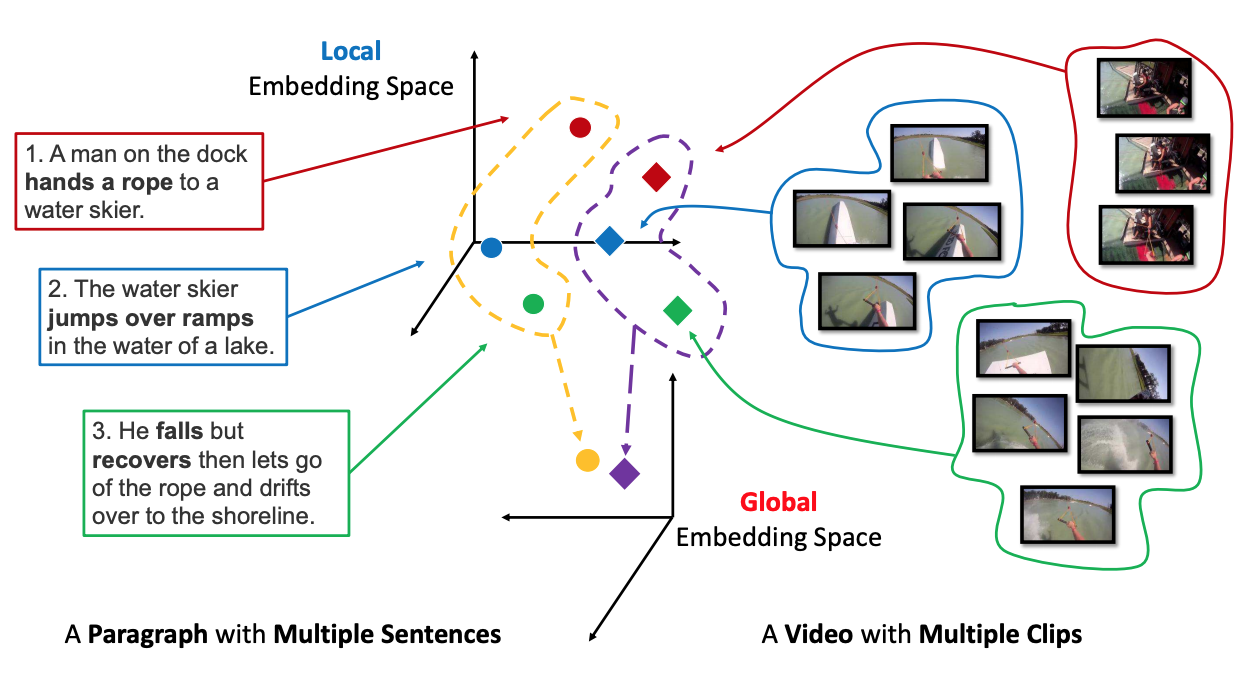
\includegraphics[width=0.9\textwidth]{images/long_vid-text.png}
    \caption{A conceptual diagram illustrates the process of modeling long-range input. The sentence/clip and paragraph/video pair is represented in local and global space respectively. \cite{zhang2018cross}}
    \label{fig:long_vidtext}
\end{figure}
Further, some works deal with long-range video-text relationship, in which video input is a set of consecutive clips, each displays a specific event and text data is a paragraph of multiple sentences describing those events in the respective order. 
Zhang et al. \cite{zhang2018cross} constructs a hierarchical architecture with different levels: video/paragraph, clip/sentence, frame/word to capture the whole temporal context, and apply losses that enforces the interaction between and within different hierarchy levels (shown in Figure \ref{fig:long_vidtext}). Ging, Simon, et al. \cite{ging2020coot} utilizes the objective function from Zhang et al. \cite{zhang2018cross} and proposes a new transformer-based architecture along with a trainable aggregation function to learn better representation. In this work, we adopt these modules to build a RL-based retrieval module, which is also used as a baseline for further improvements.\\
In some cases when the retrieval targets based on some specific details, and the video may contain abundant relations, those aformentioned methods could pay less attention to those important relations, which leads to worse performance. The RL-based architectures now need to enhance those semantic representations when modeling. Feng, Zerun, et al \cite{feng2020exploiting} address the issue by generating region features with semantic relations for frame-level embeddings. Chen, Shizhe, et al \cite{chen2020fine} proposes a hierarchy of three-level semantic matching: event level (based on whole input sentence), actions and entities denoted by verbs and noun phrases respectively. Taking inspiration from these approaches, we propose a relation module to extract semantic relationships between targets and neighboring objects.


% \section{Natural language-based vehicle retrieval}
\label{sec:ai_city}
\begin{figure}[!ht]
    \centering
    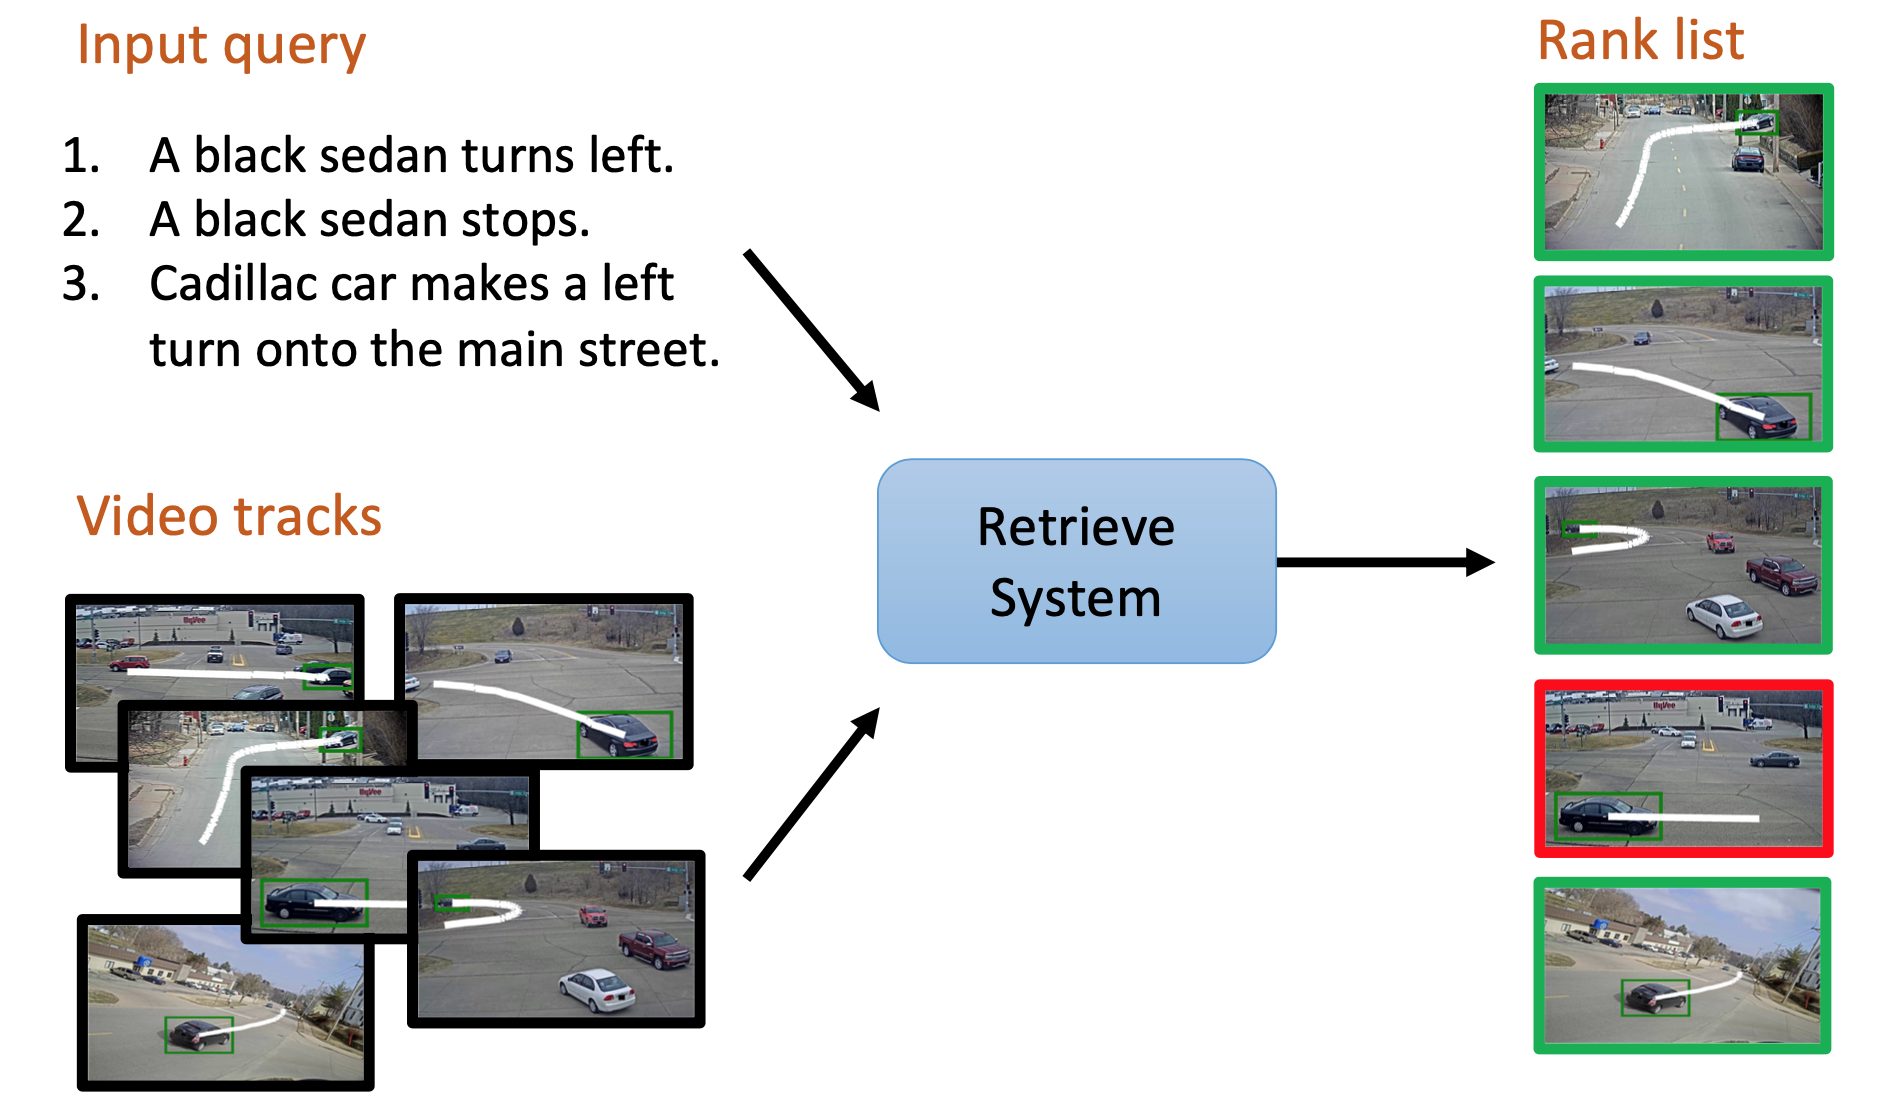
\includegraphics[width=0.9\textwidth]{resources/images/problem_statement.png}
    \caption{NLP-based traffic event retrieval workflow in the AI City Challenge 2021, Track 5.}
    \label{fig:problem_statement}
\end{figure}
In smart cities, Intelligent Traffic Systems (ITS) utilize recorded data and make use of advanced technologies to manage traffic flows, help people and goods move faster. In fact, ITS benefits from insights derived from data captured by sensors. The AI City Challenge \cite{Naphade21AIC21} provides a large video dataset capturing practical traffic scenarios with the intention of integrating intelligent video analytics into real-world deployment. The challenge also provides a scoring system for participants to evaluate their methods in both accuracy and efficiency measures. In 2020, the 5th AI City Challenge is organized with five problem tracks as follows:
\begin{itemize}
    \item \textbf{Multi-class multi-movement vehicle counting using IoT devices}: In this task, participants implement systems to count four-wheel vehicles and freight trucks following a pre-defined movements. The evaluation requires efficient algorithms able to produce accurate results in acceptable runtime. The dataset consists of 31 video clips that capture 20 unique traffic positions.
    \item \textbf{Vehicle re-identification with real and synthetic training data}: The goal of this task is to improve algorithms that identify the same vehicles from different cameras. Dataset provided this year is an extension of the previous version (CityFlowV2-ReID), containing over 85,000 variable-size vehicle images cropped from 46 different cameras. 
    \item \textbf{City-scale multi-target multi-camera vehicle tracking}: Participants perform multi-target multi-camera vehicle tracking on the dataset constructed from 880 distinct annotated vehicle identities, referred to as CityFlowV2. 
    \item \textbf{Traffic anomaly detection}: Teams participating in this track provide algorithms to detect anomalies in camera videos, such as accidents, car crashes or stalled vehicles, etc. The videos in this track are captured at highways and intersections in Iowa, USA. There are 100 videos with a total 18 anomalies for the training set and 150 videos for the test set. 
    \item \textbf{Natural language-based vehicle retrieval}: According to the organizers, this task is the first challenge that utiilizes natural language processing for such a city-scale retrieval problem. In this track, teams were asked to build systems that retrieve appropriate vehicle tracks given natural language descriptions in text. The train dataset contains about 2,500 video-caption pairs while the number is about 150 pairs for the test set (referred to as CityFlow-NL benchmark).
\end{itemize}
In this work, we utilize the Track 5 evaluation platform to experiment and validate our proposed methods on the retrieval task. To keep up with the trending solutions, we discuss some notable solutions for this track at the 5th AI City Challenge. An overview of the mentioned problem is shown in Figure \ref{fig:problem_statement}. \\
\subsection{Impressive solutions for natural language-based vehicle retrieval}
Most existing methods \cite{bai2021connecting, sun2021dun, nguyen2021contrastive, sebastian2021tied, nguyen2021traffic} in Track 5 apply representation learning based modeling for both visual and textual inputs to perform the retrieval task. Experiments indicate that ensembles of different encoder networks provide competitive results for this method.
The 3th solution \cite{park2021keyword} aims to extract descriptive attributes from input query and appearance features from vehicle track to construct a keyword-based retrieval system.

\textbf{Query modeling} \\
The common approach is to utilize pretrained transformer-based models (BERT \cite{devlin2018bert}, RoBERTa \cite{liu2019roberta}) or recurrent units (LSTM \cite{hochreiter1997long}, GRU \cite{cho2014learning}) to embed input query to perform representation semantic matching.
Bai, Shuai, et al \cite{bai2021connecting} enhances model robustness with back-translation augmentation technique.
Park, Eun-Ju, et al \cite{park2021keyword} and Nguyen, Tien-Phat, et al. \cite{nguyen2021traffic} apply conventional natural language tools to analyse the queries, extract useful cues such as vehicle type, color, motion attributes or relationships to neighboring vehicles.

\textbf{Vehicle track modeling} \\ 
Most teams first extract a sequence of frame-level features then apply a sequence model to get final representation of the video track.
Best performing team, Bai, Shuai, et al \cite{bai2021connecting} proposes dual path architecture for video embedding, when one branch aims to extract background information and target vehicle trajectory, the other focuses on the target appearance itself.
Park, Eun-Ju, et al \cite{park2021keyword} intends to build a keyword-based retrieval system that uses target vehicle type, color and movement direction. A color and vehicle classifier trained with cropped images in the given video are used for appearance categorization, while the movement behaviour is modelled from vehicle’s position and velocity vector using trajectory GPS coordinates. 
Through experiments, Park, Eun-Ju, et al \cite{park2021keyword} shows that a combination of searching essential attributes still achieves good results without using any retrieval model.
Nguyen, Tien-Phat, et al. \cite{nguyen2021traffic} applies attribute classification and trajectory-based motion detection to perform re-ranking on final retrieval results and get competitive performance.
\subsection{Conclusion}
Based on the reported results from top teams, we claim that in the vehicle retrieval problem, the targets’ attributes provided by input descriptions are important cues to determine which tracks are mentioned. 
In other words, in the video analytic stage, the algorithm should focus on how the target vehicle looks, by extracting all external attributes, motion patterns and finding out relationships with around vehicles to match with all aspects described in the input queries.
From this point of view, in this work, we propose a retrieval system based on vehicle appearance and motion attributes that achieve best performance on the CityFlow-NL benchmark. In the next sections, we discuss two important tasks utilized to extract vehicle attributes in our proposed method.



% \section{Multiple object tracking}
\label{sec:mot}
Multiple object tracking (MOT) is to perform simultaneously tracking many objects in a video through locating their positions while maintaining their identities.
MOT task plays an important in many intelligence application, which supplies a helpful tools for complicated analysis works, such as video surveillance, safety monitoring or instance behavior understanding, etc.
Contemporary MOT methods follow the tracking-by-detection paradigm: extract set of detections from consecutive video frames then associate them to construct target tracklets. Therefore, many researches \cite{bergmann2019tracking,zhou2020tracking,bochinski2017high,bewley2016simple} show that if the detectors work well, they provide strong information cues to associate objects, hence boost the tracking performance. 
In general, tracking-by-detection MOT algorithms share parts of the following steps:
\begin{itemize}
    \item \textbf{Detection stage}: an object detectors is utilized to locate all potential objects which could be appearance of our concerned targets.
    \item \textbf{Feature Extraction stage}: apparent or motion feature represents each detected objects is extracted for further comparison.
    \item \textbf{Similarity Measure stage}: Representation features are used to compute similarity/distance score between detected tracks so far and new detections.
    \item \textbf{Association stage}: assign target ID to detected objects based on matching scores from previous steps.
\end{itemize}
\begin{figure}[t!]
    \centering
    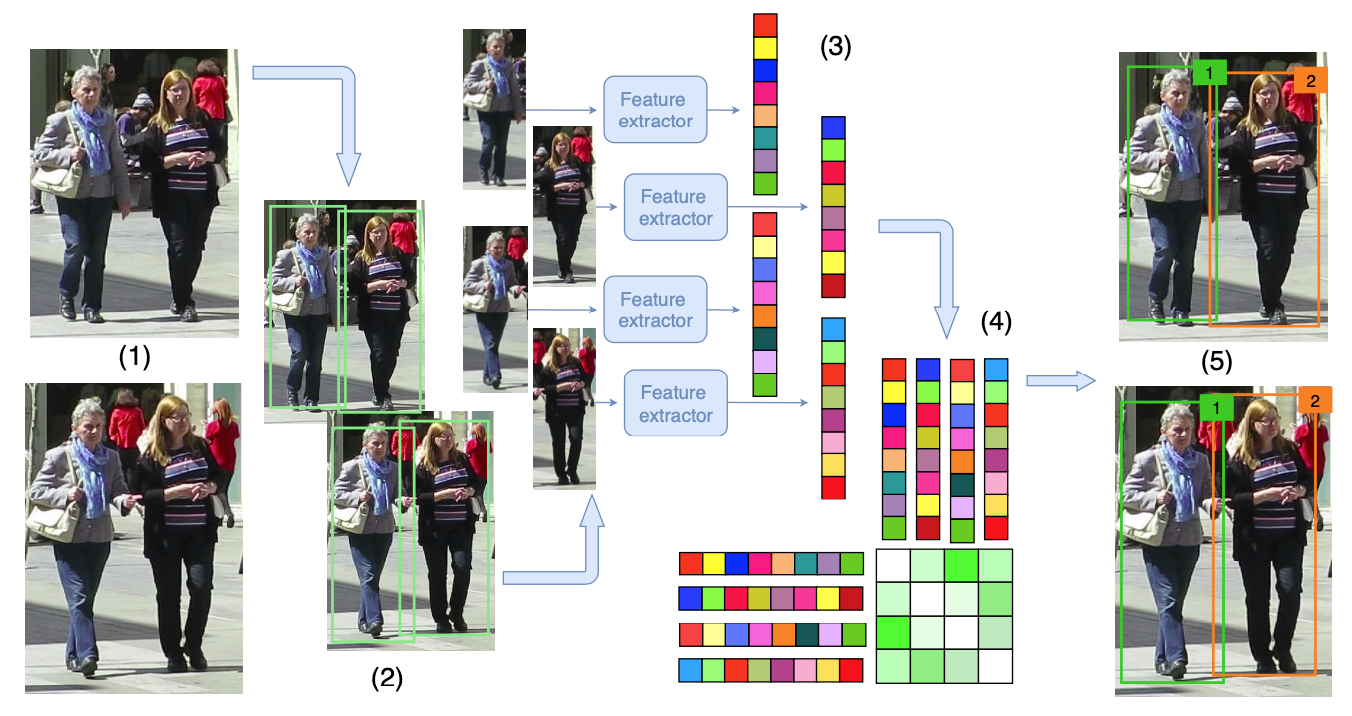
\includegraphics[width=0.9\textwidth]{images/MOT_overview.png}
    \caption{An overview of common MOT algorithms workflow. For each consecutive frames (1), the algorithm first detect all potential objects (2), then extract their representation features (3) and adopt pair-wise comparison (4) to associate most similar objects with the same ID (5). \cite{ciaparrone2020deep}}
    \label{fig:MOT_overview}
\end{figure}
Figure \ref{fig:MOT_overview} shows the step-by-step procedure of common MOT approaches.\\
Common algorithms solved MOT problem can be divided into two main groups: offline and online methods. 
Offline learning (batch based tracking) \cite{rezatofighi2015joint,kim2015multiple} assumes that the system has seen the whole video before start processing. 
Online learning approaches are only allowed to process and update tracking results frame by frame. Due to the efficiency and practicality, online and realtime algorithms achieves more attention. Many works \cite{pang2021quasi, zhou2020tracking, bergmann2019tracking, wojke2017simple} have been proposed to explore this type of learning and achieve potential results on benchmark settings and in practical situations. 
% In the scope of this project, we modified the DeepSORT \cite{wojke2017simple} method as a submodule for our retrieval system.

\subsection{SORT algorithm}
\label{sec:sort}
We first briefly discuss one of the most popular online tracking method, which successfully leverage ConvNet for detection step to achieve state-of-the-art result at the time it proposed, the Simple Online and Realtime Tracking (SORT) \cite{bewley2016simple} algorithm.
The important features of SORT compose: target detections based on Faster-RCNN \cite{NIPS2015_14bfa6bb} architecture, the use of Kalman filter \cite{kalman1960new} to forecast target positions at each time step and Hungarian algorithm \cite{kuhn1955hungarian} for the similarity matching step between current tracks and new detected objects. These modules help to achieve potential accuracy while greatly improves the speed of tracking multiple targets at the same time. \\
\begin{figure}[t!]
    \centering
    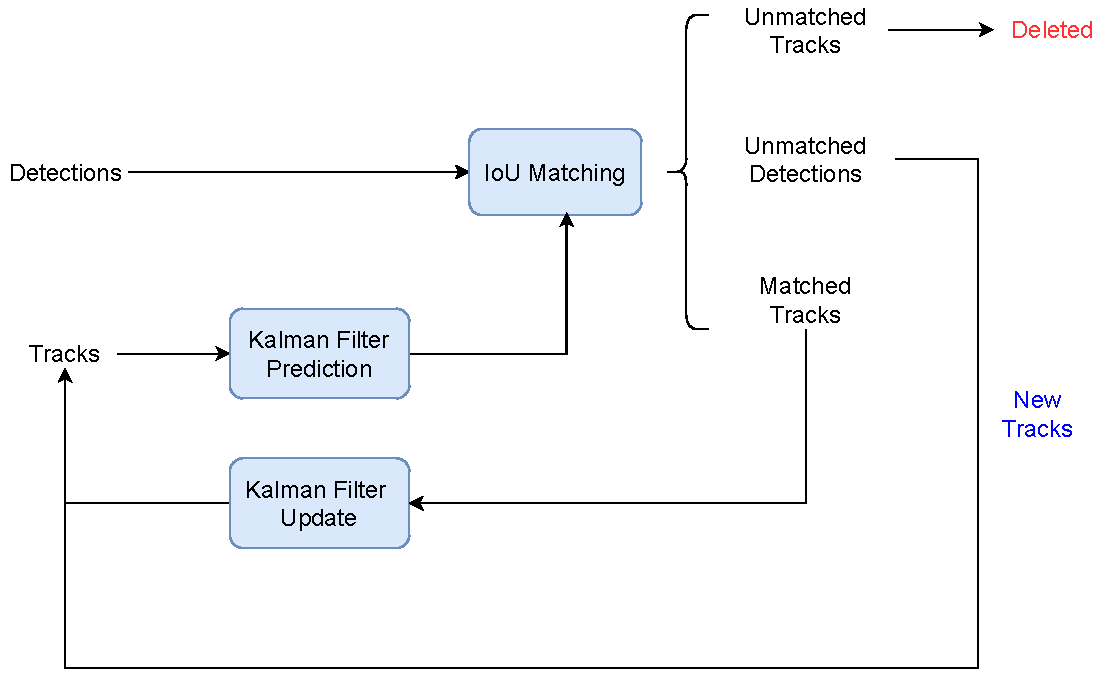
\includegraphics[width=0.9\textwidth]{images/SORT.pdf}
    \caption{SORT algorithm's processing flow.}
    \label{fig:SORT_overview}
\end{figure}
At each time step $t$-th, let $T$ denotes list of tracks we have successfully associate so far, the SORT algorithm works as follow:
\begin{itemize}
    \item \textbf{Detection stage}. \\
    The method utilizes an detector model to detect all potential objects current frame. Suppose that we have $N$ boxes at this frame.
    
    \item \textbf{Kalman Filter prediction stage}. \\
    For each track in $T$, Kalman Filter uses those movement states from previous frames to predicts the target position and speed at current frame. 
    The SORT algorithm works with assumptions that all targets have linear constant velocity and their movements are independent with the others. Hence, a state of target object at a specific time step is implemented as follow.
    \begin{align}
        \label{eqn:sort_kf}
        \mathbf{x} = [u,v,s,r,\dot{u},\dot{v},\dot{s}]
    \end{align}
    where $u, v$ represents the horizontal and vertical coordinate of the target center respectively. While $s$ is the bounding box area and $r$ is the corresponding aspect ratio. $\dot{u},\dot{v},\dot{s}$ denotes the velocity of those values at current time $t$.
    \item \textbf{IOU matching stage}. \\
    Those predicted states at current frame are used to compute a similarity matrix between $T$ tracks and $N$ detected boxes based on IoU score, result in a similar matrix of size $[N \times T]$. Hungary algorithm is then applied on this matrix to produce best matching detection for each track.
    \item \textbf{Confirmation stage}. \\
    Those with similarity score is higher than a threshold are considered as \textit{matched tracks}. Otherwise, tracks with small similarity are seen as disappear from current frame and removed from the system memory. Detections that are not currently matched with any tracks are used to initialize as \textit{new tracks} and saved to the memory.
    \item \textbf{Kalman Filter Update stage}. \\
    The predicted and observed values of matched tracks are linearly weighted to update the current state representation.
\end{itemize}
Figure \ref{fig:SORT_overview} illustrates the workflow of SORT algorithm at each frame.\\
However, SORT algorithm still have some drawbacks when running on those hard cases. The first problem is with the linear assumption of Kalman Filter framework, in practice, the targets rarely move with constant velocity.
And second, ID switches is the biggest drawback of SORT. The association between detections and tracks is simply based on IoU measure, which indicates that the algorithm only cares about the object shape, this causes the phenomenon that the number of ID switches of an object is extremely large when the object is obscured or when the trajectory overlaps with the others.

\subsection{Deep SORT algorithm}
\label{sec:deep_sort}
In this section, we consider another tracking approach that built as an extension to SORT algorithm, Deep SORT \cite{wojke2017simple}. To address the disadvantages of SORT, Deep SORT utilize deep learning network to extract features of detected objects to enhance the data association process. Furthermore, a matching cascade strategy with a new confirmation strategy is proposed to handle the problem of occlusion tracks. These improvements are shown in figure ... .
As compare to figure(SORT), Deep SORT adds a \textit{Matching Cascade} module and a new trajectory confirmation strategy to the original SORT algorithm. \\
To handle the occlusion problem, Deep SORT manages life-cycle of each archived track based on a state variable with three values (\textit{tentative}/\textit{unconfirmed}, \textit{confirmed}, \textit{deleted}). 
\begin{itemize}
    \item Each new track is initialized as \textit{unconfirmed}. Through the filtering process, if the track is not removed in the next three frames, it becomes \textit{confirmed} track, and will stay filtered for the next $max\_age$ frames.
    \item Otherwise, if the track is lost when less then 3 frames are reached, it will be deleted.
\end{itemize}

\begin{figure}[t!]
    \centering
    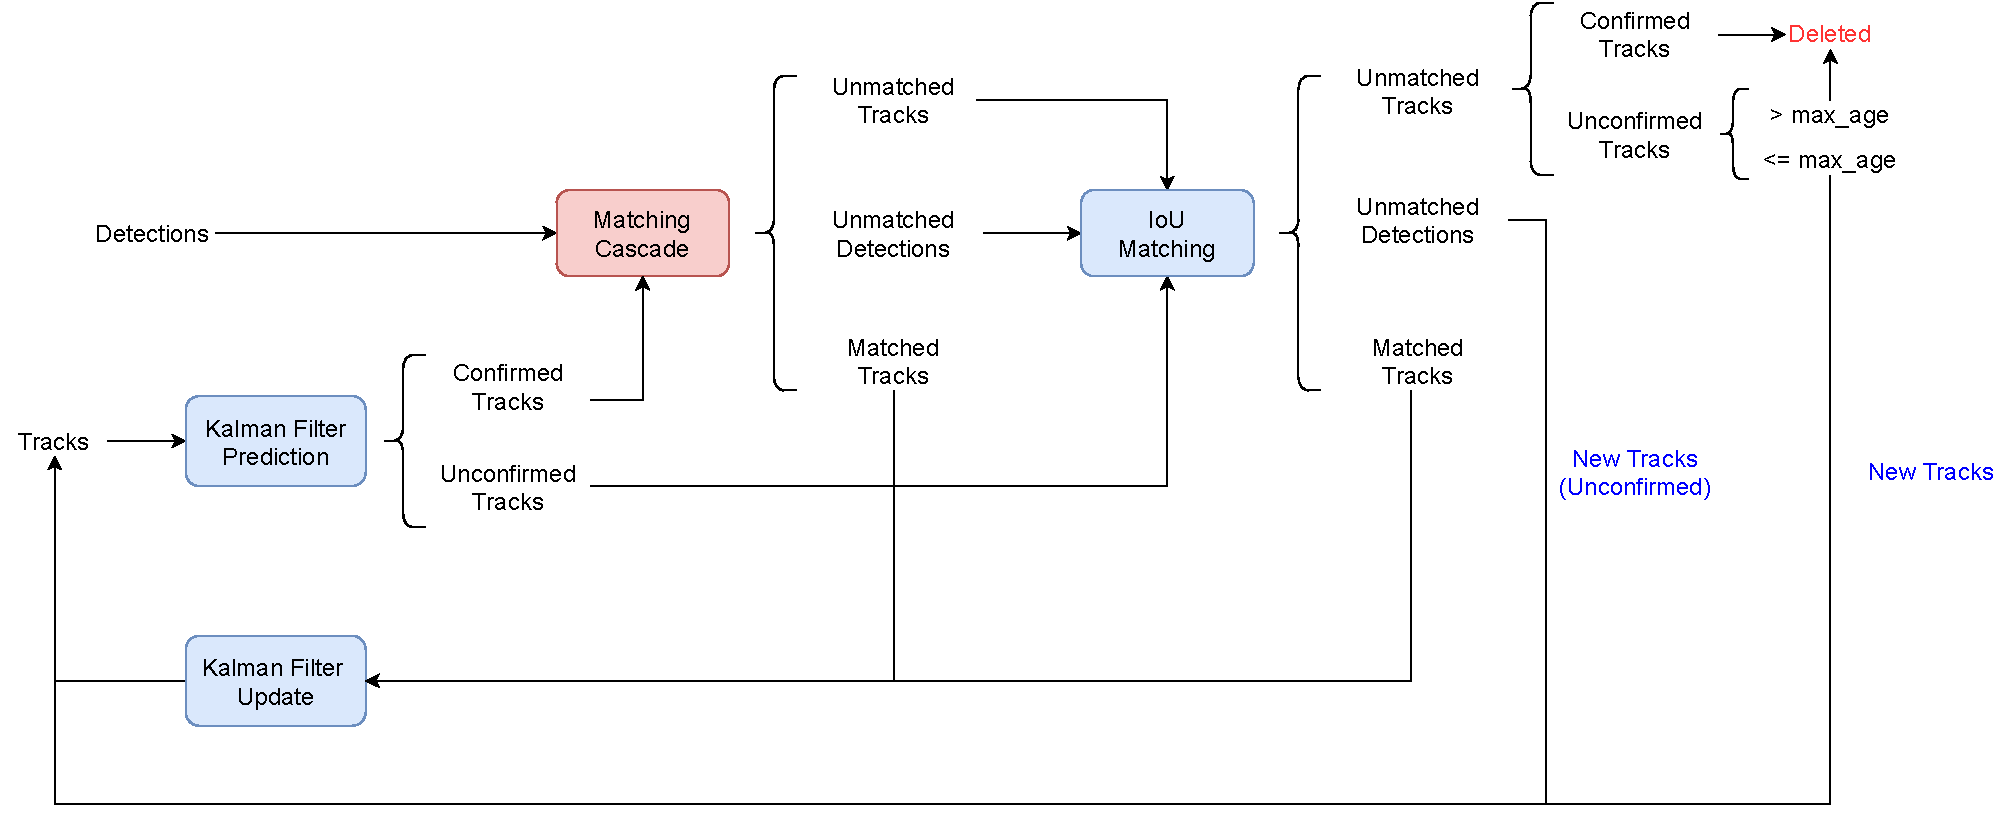
\includegraphics[width=\textwidth]{images/DeepSORT.pdf}
    \caption{Deep SORT algorithm's processing flow.}
    \label{fig:DeepSORT_overview}
\end{figure}

The details of each stage in Deep SORT process are described as follows (shown in figure \ref{fig:DeepSORT_overview}).
\begin{itemize}
    \item \textbf{Detection stage}. \\
    Same as SORT algorithm, Deep SORT use an object detector to detect all potential boxes at current frame.
    \item \textbf{Kalman Fitler Prediction and Update stage}. \\
    Same as SORT algorithm, predict next representation to perform prediction and update current state if finding new detection for each track.
    \item \textbf{Filter Layer 1: Matching Cascade}. \\
    The Matching Cascade takes in a list of archived tracks $T$ and assign them to best matching objects from $N$ detections at current frame. Different from the original SORT, Deep SORT integrates both motion feature and appearance feature to measure the similarity. 
    Motion feature is modelled the same way as the SORT algorithm (\ref{eqn:sort_kf}), while the appearance descriptor is extracted from pretrained CNN-based network trained with re-identification settings. 
    In general, the similarity measure between track $i$ and object $j$ is formulated as follow
    \begin{align}
        \label{eqn:deepsort_score}
        c_{i,j} = \lambda d_{motion}(i, j) + (1-\lambda) d_{appearance}(i, j)
    \end{align}
    Where Mahalanobis distance is used to measure motion uncertainty $d_{motion}$ and Cosine distance is used for appearance measure $d_{appearance}$. \\
    With the computed similarity matrix, Deep SORT then applies multi-step thresholding on archived tracks based on their ages, and finally produce list of matched tracks, unmatched detections and unmatched tracks.
    \item \textbf{Filter Layer 2: IoU Matching}. \\
    This filter apply IoU association with the same strategy as SORT on unlinked tracks and detections from previous layer and archived unconfirmed tracks. 
    \item \textbf{Confirmation stage}. \\
    After the two layers of filtering, unconfirmed tracks that still not match with any detections of confirmed tracks which have stayed too long in the memory (larger than $max\_age$) are removed. Unmatched detections are used to create new tracks and the procedure starts over with the next frame.
\end{itemize}
In the scope of this project, we modified the DeepSORT algorithm \cite{wojke2017simple} to utilize as a sub-module that captures the relationships between target object and neighboring vehicles.

% \section{Semantic Role Labeling}
\label{sec:srl}
Semantic Role Labeling (SRL) task aims to perform semantic analysis of texts that analyzes the propositions expressed by all target verbs of the sentence. 
For each target verb (also known as predicate), all constituents (or arguments) related to that verb are assigned semantic role labels. In common, the task is to extract predicate-argument structure for input sentences to answer the question “who did what to whom, when, where, how and why ?”.
Common solutions for the SRL can be treated as a classification problem performed on each part of the input sentence. 
The methods  aim to classify each part into correct semantic roles with respect to the predicates. \\
Many deep neural networks were proposed to solve the problem with or without detected predicates \cite{zhou2015end, marcheggiani2017simple, he2017deep, tan2018deep, he2018jointly, strubell2018linguistically}. 
The main approach is to apply the sequential models to learn the representations for each input part, then perform classification into a pre-defined set of roles.\\ 
As mentioned in section \ref{sec:BERT}, BERT is a powerful pretraining for such language modeling tasks. Shi, Peng, and Jimmy Lin.\cite{shi2019simple} proposed a BERT-based model to solve the SRL problem and achieve state-of-the-art results on different benchmarks. The method is then applied in various video-text related problems to implement such fine-grained models (discussed in section). 
\begin{figure}[t!]
    \centering
    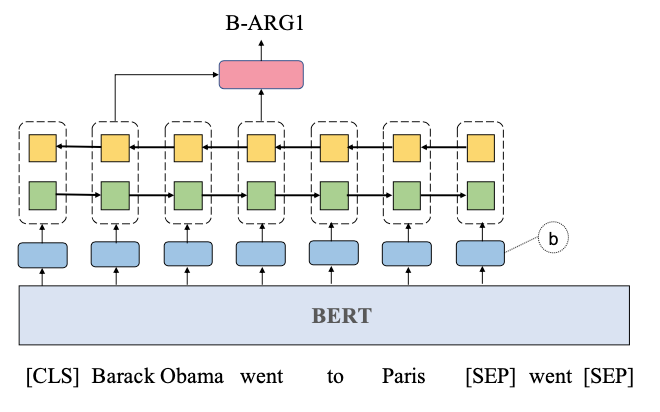
\includegraphics[width=0.7\textwidth]{images/SRL_overview.png}
    \caption{An example of the BERT-based SRL method \cite{shi2019simple} making prediction for the token "Barack".}
    \label{fig:srl_overview}
\end{figure}
The architecture is constructed from BERT encoding followed by a BiLSTM layer, and a one-hidden-layer MLP to produce prediction for each tokens. In more details, the process is as follows (illustrated in figure \ref{fig:srl_overview}):
\begin{itemize}
    \item Given a pair of sentence-predicate $(X, p)$ as input, the input sequence is encoded as [[CLS] sentence [SEP] predicate [SEP]]. This method allows the predicate representation to interact with the whole input context via the self-attention mechanism.
    \item The encoded sequence is then fed into BERT encoder to obtain the sentence representations from [[CLS] sentence [SEP]] tokens. The predicate indicator embedding $\mathbf{b}$ is also associated to locate the predicate positions in the sentence.
    \item The sentence representations are then fed through a BiLSTM layer to get the final representation of each token. 
    \item Finally, to get semantic role prediction for each token, the final hidden state of predicate $\mathbf{h_p}$ is concatenated to that token hidden state $\mathbf{h_i}$ and fed into a feed-forward classifier layer over the pre-defined role set.
\end{itemize}

\textbf{SRL in vision} 
\begin{figure}[!htb]
    \centering
    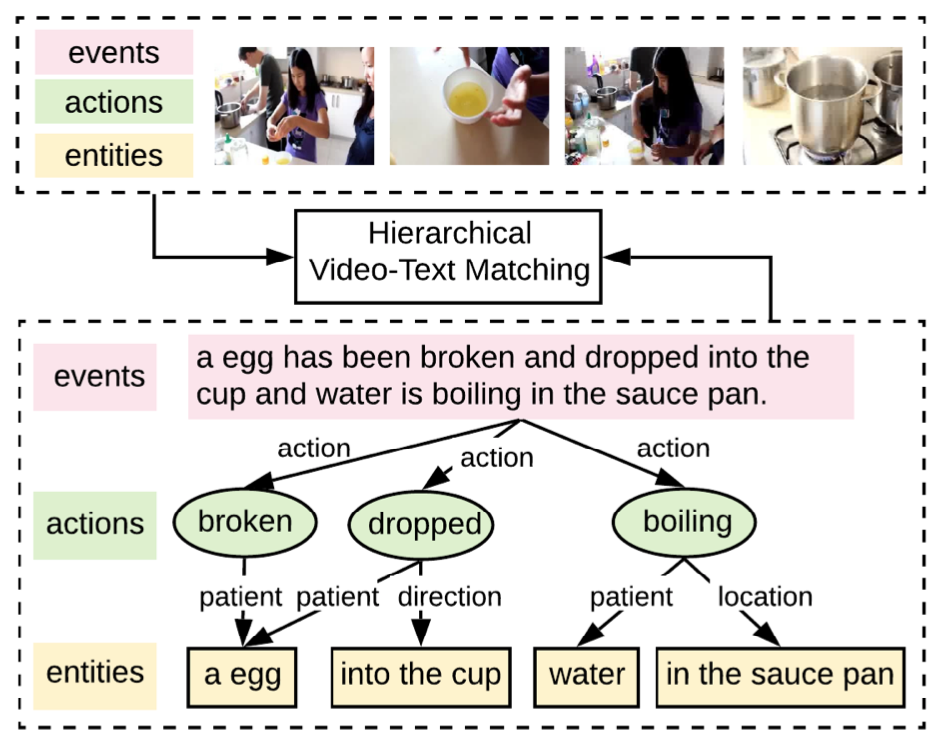
\includegraphics[width=0.7\textwidth]{images/HGR_idea.png}
    \caption{The overview of HGR\cite{chen2020fine} matching process.}
    \label{fig:hgr_overview}
\end{figure}

The SRL task attracts much attention from researchers and has been widely applied in video analytics, where it provides fine-grained cues for matching textual description to correct visual context, such as human object interaction \cite{gupta2015visual}, video question answering \cite{sadhu2021video}, or video grounding \cite{sadhu2020video}, etc. The most related to ours is the utilization of SRL in video-text retrieval. Chen, Shizhe, et al. \cite{chen2020fine} proposed a Hierarchical Graph Reasoning (HGR) model to performs fine-grained retrieval task in many levels (shown in figure \ref{fig:hgr_overview}).
For each input sentence, Shizhe, et al. \cite{chen2020fine} first applies the SRL toolkit \cite{shi2019simple} to obtain predicates and their related semantic role then construct a three-level role graph, including events, actions and entities levels. 
The event node contains the whole input sentence to represent the global context, connected by action nodes that contain the extracted predicates context. The other noun phrases are entity nodes connected to different action nodes. The directed edges between action nodes and entity nodes indicate their semantic role relation.\\
In our work, the input query describes different attributes of the target objects, we apply SRL toolkit\cite{shi2019simple} to extract these signals to perform refinement and re-ranking to enhance the retrieval results.




\section{Segmentation}
\label{sec:segmentation}
Segmentation is one of the most important tasks in image processing and has a long history of development. It has grown strongly since neural networks and computing resources starting to explode. One of the basic ideas behind segmentation is that you can use convolution layers as a feature extraction mechanism. By downsampling the input image after passing it through a backbone CNN model containing multiple pooling layers, you can generate a prediction at a smaller scale that needs to be upsampled to the original image size. This approach, which uses fully convolutional layers to perform classification for each pixel in the feature map, is known as Fully Convolutional Networks (FCNs)\cite{FCN}.

The reason behind this architecture that combine deep semantic information in deeper layers and spatial information in shallow layers together. However, there are still many limitations, such as losing spatial information in the downsampling process; its inability to leverage global context information; and the lack of a mechanism for variant-scales.

The next popular method is using encoder and decoder based architecture. Segnet\cite{segnet} is the pioneer when do a symmetric architecture between encoder and decoder. In details, decoder mirror copy of the decoder and augment with information from encoder. There are multi descendants inspire from this and popular nowadays like Unet\cite{Unet}

Unet\cite{Unet} is one of the most popular architectures in computer vision, and it has been shown to be very effective in medical applications. The encoder provides spatial information that helps to decode the features more accurately. There are variants of Unet that have been developed specifically for better performance, such as Unet++\cite{UnetPP} and Attention U-Net\cite{AttUnet}. These variants continue to show promise for semantic segmentation tasks, with improved accuracy over other methods.

Another model to approach the fixed kernel size problem is of the family of segmentation models called DeepLab\cite{Deeplab}. DeepLab model family is a promising solution to the fixed kernel size problem. They use dilated convolution (also known as atrous convolution) to learn features from a larger region without increasing computational expenses. This allows for deeper neural networks, which can better capture complex patterns in data. Atrous Convolutions with different rates are stacked in the encoder, called the Atrous Spatial Pyramid Pooling module. This module offers the ability to learn multi-scale features in the encoding phase, which is important for accurately capturing information about objects and scenes.

Computer vision has come a long way in the past few years. Researchers have found that transformer power is one of the potential ways to improve computer vision. Transformers are famous for their ability in downstream task in natural language processing. However, the naive usage that replaces transformer vision as a feature extraction is not exploiting almost its capability. Due to that TransUnet\cite{TransUnet} use the strong point of them ideas, which is transformer leverage both detailed high-resolution spatial information from CNN features and the global context encoded by Transformers, also inspired by the u-shaped architectural design 

\section{Uncertainty Estimation}
\label{sec:uncertainty}

Data is growing bigger everyday, but that is still not enough for deep neural networks. The empirical report of \cite{mahajan2018exploring}, \cite{joulin2016learningvisual} suggests that the performance of recent deep networks is not yet saturated with respect to the size of training data, since data are mostly unlabeled. For this reason, learning methods from semi-supervised learning to unsupervised learning are attracting attention of many researchers. However, given a fixed amount of data, performance of semi-supervised or unsupervised still cannot match with that of fully-supervised learning. 
Thus, the data annotation has a vital part in uplifting the performance of neural networks
Having said that, what then is the suitable approach while the budget for annotation is limited?  \cite{atlas1989trainingconnectionist} first proposed active learning where a model actively selects data points that the model is uncertain of. The core idea of active learning is that the most informative data point would be more beneficial to model improvement than a randomly chosen data point.

Active learning has been advancing in the recent decades. Given a scenario where a labeled dataset \mathcal{L} and an unlabeled dataset \mathcal{U} is available, active learning aims to select a fixed number of subset of samples from \mathcal{U} to be labeled such that they can lead to improvement in model performance. To identify the most valuable examples to be labeled, many sampling strategies have been proposed in previous research, and it is mostly the main focus of those. Data points chosen by these strategies are expected to be able assist model to become more generalized and comprehensive after training.

Given a pool of unlabeled data, there have been two major approaches according to the selection criteria: uncertainty-based, diversity-based and expected model change

Uncertainty-based strategy [\cite{joshi2009multi}, \cite{wang2016cost}, \cite{tong2001svmactive}, \cite{seung1992query}, \cite{beluch2018power}] selects samples for which the model produces most uncertain predictions while the diversity approach [\cite{sener2018activelearningforcnn}, \cite{nguyen2004activepreclustering}, \cite{guo2010activeinstance}] selects diverse data points that can represent the entire distribution of the unlabeled pool.
Expected model change [\cite{roy2001toward}, \cite{settles2007multiple}, \cite{freytag2014selecting}] selects data points that brings great impact to the training model parameters or its outputs.

The most straightforward method of the uncertainty approach is to utilize class posterior probabilities to define uncertainty. Despite its simplicity, this approach has performed remarkably well in various tasks, such as object detection \cite{wang2018towardshuman}, semantic segmentation \cite{jain2016activesegmentationprop} and human pose estimation \cite{liu2017activehumanpose}.

Recently, Gal et al. \cite{gal2017deep} obtains uncertainty estimation from deep networks through multiple forward passes by Monte Carlo Dropout \cite{gal2016dropout}. It was shown to be effective for classification with small datasets, but according to [32], it does not scale to larger datasets.

Interestingly, \cite{yoo2019learningloss} train an additional regression module, which uses the training loss as optimization target, to predict a score for each unlabeled sample to evaluate its worthiness for labeling. 

The majority of empirical results from previous researches suggest that active learning is actually reducing the annotation cost. The problem is that most of methods require task-specific design or are not efficient in the recent deep networks.

\begin{figure}[h]
    \centering
    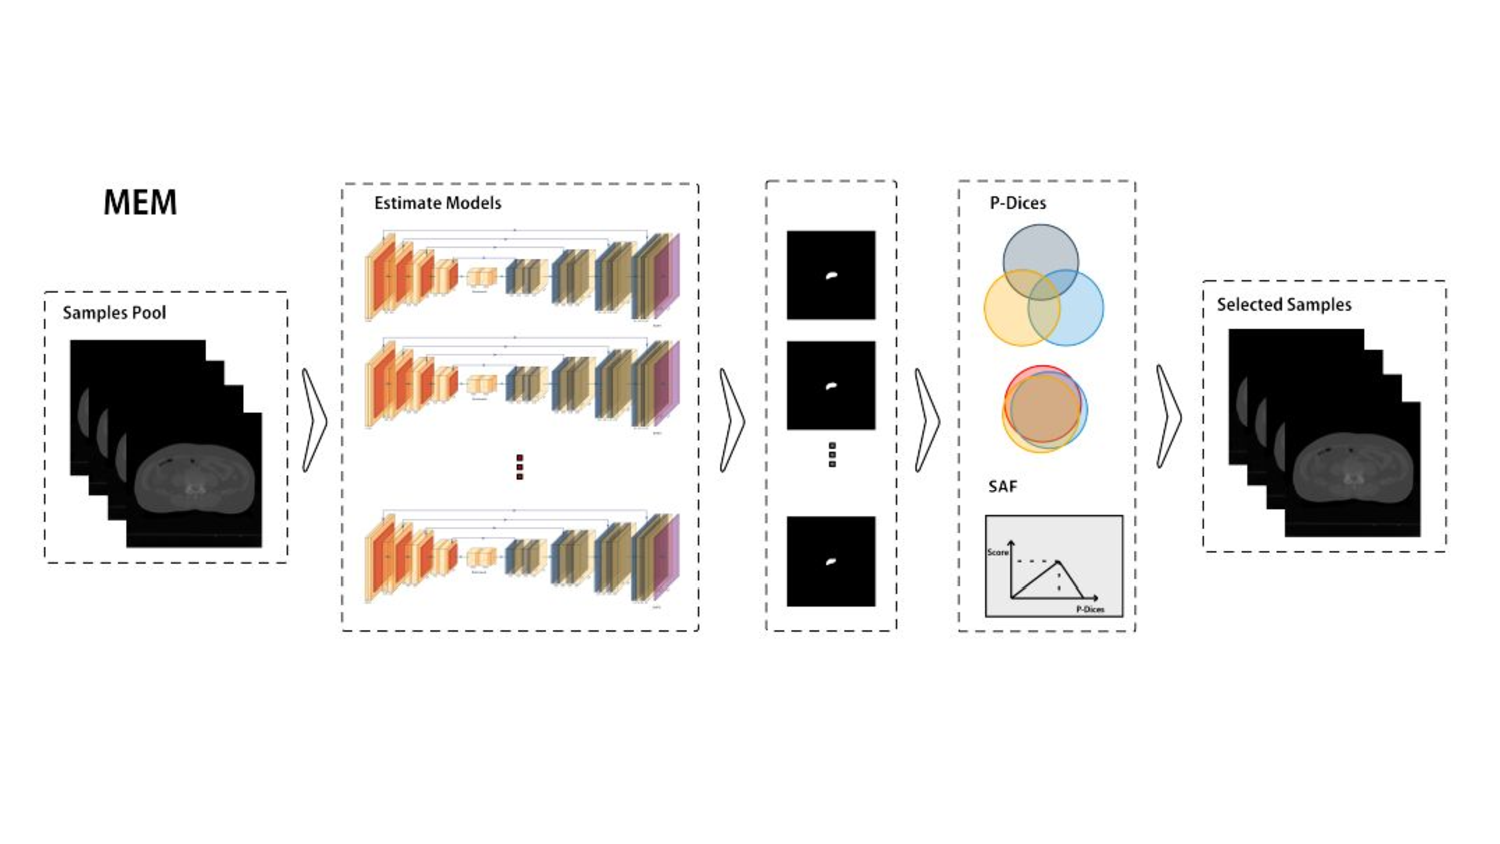
\includegraphics[width=\textwidth]{content/resources/new_images/related_works/pdices.pdf}
    \caption{A pipeline for active learning proposed in \cite{wang2019twostagequery}, which calculate unlabeled sample score through the two-step query strategy: P-Dices and SAF}
    \label{fig:pdices}
\end{figure}

As a task-agnostic uncertainty approach, \cite{seung1992query}, \cite{beluch2018power} train multiple models to construct a committee, and measure the consensus between the multiple predictions from the committee. \cite{wang2019twostagequery} goes with the same strategy where the authors compute the entropy between numerous trained agents, as depicted in Figure \ref{fig:pdices}.

We follow \cite{wang2019twostagequery} to use deep ensemble to generate prediction for each unlabeled sample, then based on consensus entropy to select good samples. While previous works aim at finding the most uncertain samples to be manually labeled by experts, but in our context, manual annotation is forbidden, therefore we try to find most certain samples that can be used for retraining.
\section{Semi-supervised learning}
\label{sec:semisup}

With the constantly increasing volume of non-annotated raw data in practice, semi-supervised learning approaches have been gaining popularity in the area of deep learning recently to effectively utilize this source of data.  
Recent works focus on two of the most common semi-supervised methods, which are consistency regularization and pseudo-labeling.

Consistency regularization aims at enforcing the consistency between the predictions (or intermediate features) of two different views of an unlabeled input sample. 
Some prior works \cite{kim2020structuredloss}, \cite{french2019semi} add perturbation to the input sample, then forward both the original and perturbed one through the same network to generate two augmented outputs. These two outputs are forced to be similar by the regularization function. This approach can be seen as attaching an unsupervised branch to the supervised learning paradigm.

On the other hand, pseudo-labeling, a.k.a., self-learning, self-labeling, or decision-directed learning, is initially developed for using unlabeled data in classification. Recently, it is applied for semi-supervised segmentation \[\cite{zheng2021rectifying}, \cite{chen2020naivestudent}, \cite{zhu2020improving}, \cite{zoph2020rethinking} \], . Frequently, it involves more than one model to produce pseudo-labels by converting model predictions on unlabeled samples into soft or hard labels as optimization targets for retraining. The process can be iterated several times. Various schemes are introduced on how to decide the pseudo segmentation maps. For example, the GAN-based methods [\cite{hung2018adversarial}, \cite{mittal2019semi}, \cite{souly2017semisupervised}], use the discriminator learned for distinguishing the predictions and the ground-truth segmentation to select high-confident segmentation predictions on unlabeled images as pseudo segmentation.

One common type of approach is teacher-student settings. The teacher, which usually is the larger network, is fully-supervisedly trained on the labeled data while generating pseudo-labels on unlabeled data to guide the student model to learn more stably \[\cite{tarvainen2017meanteachers}, \cite{cui2019semisupervised}, \cite{hang2020localnglobal}, \cite{wang2020double}, \cite{yu2019uncertainty}\]. Often, The teacher's parameters are updated using an exponential moving average from the student's parameters \cite{cui2019semisupervised}. 

Apart from the teacher-student paradigm, many proposals are the variance of it. As discussed in \cite{ke2019dualstudent}, because of exponential moving average, teacher network in mean-teacher tends to be very close to the student when the training process converges.

Dual-student [\cite{hang2020localnglobal}, \cite{ke2020guided}, \cite{cao2022adversarial}], for instance, is proposed to use two independently initialized student network without teacher and has been achieving great performance as well. One examplar is \cite{chen2021semisupervised}, which has been adopted in our work, trains 2 segmentation models simultaneously on both labeled and unlabeled data. Basically, with two source images as input, they generate a cutmix version by combining them as one image and mixing the two pseudo segmentation maps obtained from the models. Afterward, the mixed pair of image and mask is used as supervision of the two segmentation networks. 
Developed from that, \cite{luo2021semisupervised} incorporates the idea that those two models should have different architectures to boost the performance by far, one of them should be conventional CNNs while the other has a transformers-based structure. 

Recently, SSL has been widely used for medical image computing to reduce the
annotation efforts [\cite{hang2020localnglobal}, \cite{li2020transformation}, \cite{ma2020active}, \cite{peng2020mutual}]. Bai et al \cite{bai2017semisupervised} developed an iterative framework where in each iteration, pseudo labels for unannotated images are predicted by the network
and refined by a Conditional Random Field (CRF) then the new pseudo labels are used
to update the network. 

We desire to build the same framework as \cite{bai2017semisupervised} in which multiple models, in which choosen architectures are inspired from \cite{luo2021semisupervised}, are used to refine the pseudo labels. 

However, one inherent weakness of the pseudo label learning is that the pseudo label usually contains noisy predictions. Despite the fact that most pseudo labels are correct, wrong labels also exist, which could compromise the subsequent training. If the model is fine-tuned on the noisy label, the error would also be transferred to the
adapted model. Therefore, we also integrate active learning to decide which pseudo labels are suitable for retraining the	 model.
\section{Mask Propagation}
\label{sec:mask_propagate}

Video object segmentation is a task that requires specific objects to be segmented in a given video. In terms of Semi-supervised settings, a first-frame annotation is provided by the user, and the method segments objects in all remaining frames automatically. This technique, which uses a mask as prior knowledge to predict other masks, is called Mask Propagation.

To propagate these sparse labels through the entire video sequence, traditional methods often solve an optimization problem with an energy defined over a graph structure \cite{badrinarayanan2010label}, \cite{vijayanarasimhan2012active}, \cite{avinash2014seamseg}.

Early deep neural network methods rely on fine-tuning the networks at test time to make segmentation networks focus on target objects and then inference on all other frames, which are extremely slow. Among them, OSVOS \cite{caelles2017one} and MoNet \cite{xiao2018monet} finetune pre-trained networks on the first-frame ground-truth at test time. OnAVOS \cite{voigtlaender2017online} extends the first-frame fine-tuning by introducing an online adaptation mechanism. Following these approaches, MaskTrack \cite{perazzi2017learning} and PReM \cite{luiten2018premvos} utilize optical flow to help propagate the segmentation mask from one frame to the next. Despite achieving promising results, the test-time fine-tuning restricts networks’ efficiency. 
Faster approaches have been proposed such as temporal CNN, capsule routing \cite{duarte2019capsulevos}, tracking, space-time matching, and memory-based methods:

\textbf{Temporal CNN}. Recurrent methods propagate information often from the most recent frames, either via a mask \cite{perazzi2017learning} or via a hidden representation \cite{ventura2019rvos}, \cite{hu2017maskrnn}. These methods are prone to drifting and struggle with occlusions.

\textbf{Tracking}
In contrast, tracking-based approaches \cite{jang2017online}, \cite{wang2019fast}, \cite{chen2020state} perform
frame-to-frame propagation and are thus efficient at test-time. They however lack long-term context and often lose track after object occlusions.

\textbf{Space-time matching}. While some methods \cite{huang2020fast}, \cite{voigtlaender2019feelvos} \cite{yang2020collaborative} also include the first reference frame for global matching, the context is still limited and it becomes harder to match as the video progresses

\textbf{Memory-based}. To address the context limitation, recent state-of-the-art methods use more past frames as feature memory \cite{oh2019stm}, \cite{duarte2019capsulevos}, \cite{huang2020fast} ,\cite{ge2021video}, \cite{cheng2021stcn}, \cite{cheng2022xmem}, \cite{yang2022associating}. These approaches leverage a memory network to embed past-frame predictions into memory and apply non-local attention mechanisms to propagate object information from the memory to the current frame. Our work strongly adopts the memory-based style. 

Oh et. al \cite{oh2019stm} introduces a framework which extract embeddings from multiple intermediate frames and store inside the memory. Then in forwarding stage, these memories are combined with the query embeddings to segment the object

\begin{figure}[!h]
    \centering
    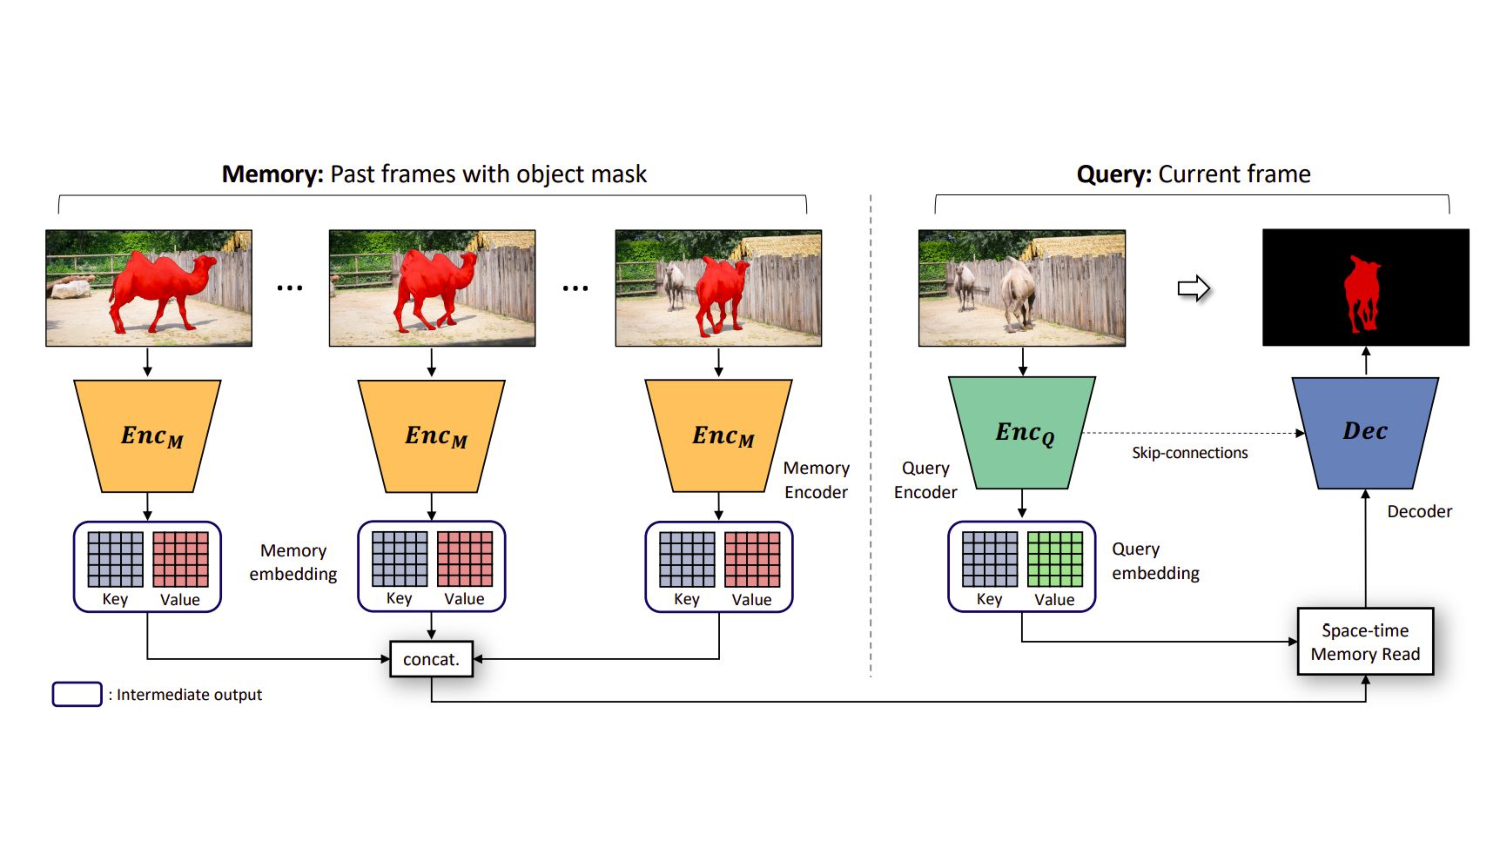
\includegraphics[width=\textwidth]{content/resources/new_images/models/stm.pdf}
    \caption{Overview architecture of STM \cite{oh2019stm}.}
    \label{fig:stm}
\end{figure}

Cheng et. al  \cite{cheng2021mivos} proposes a framework in which the user initially scribbles a mask of an object, the scribble is transformed into the real binary mask (S2M), then that mask is propagated through every video frame based on STM \cite{oh2019stm}. Then the user can choose some incorrect frames and scribble to guide the fusion with the propagated frame to output more accurate masks (Different-aware fusion).

\begin{figure}[!h]
    \centering
    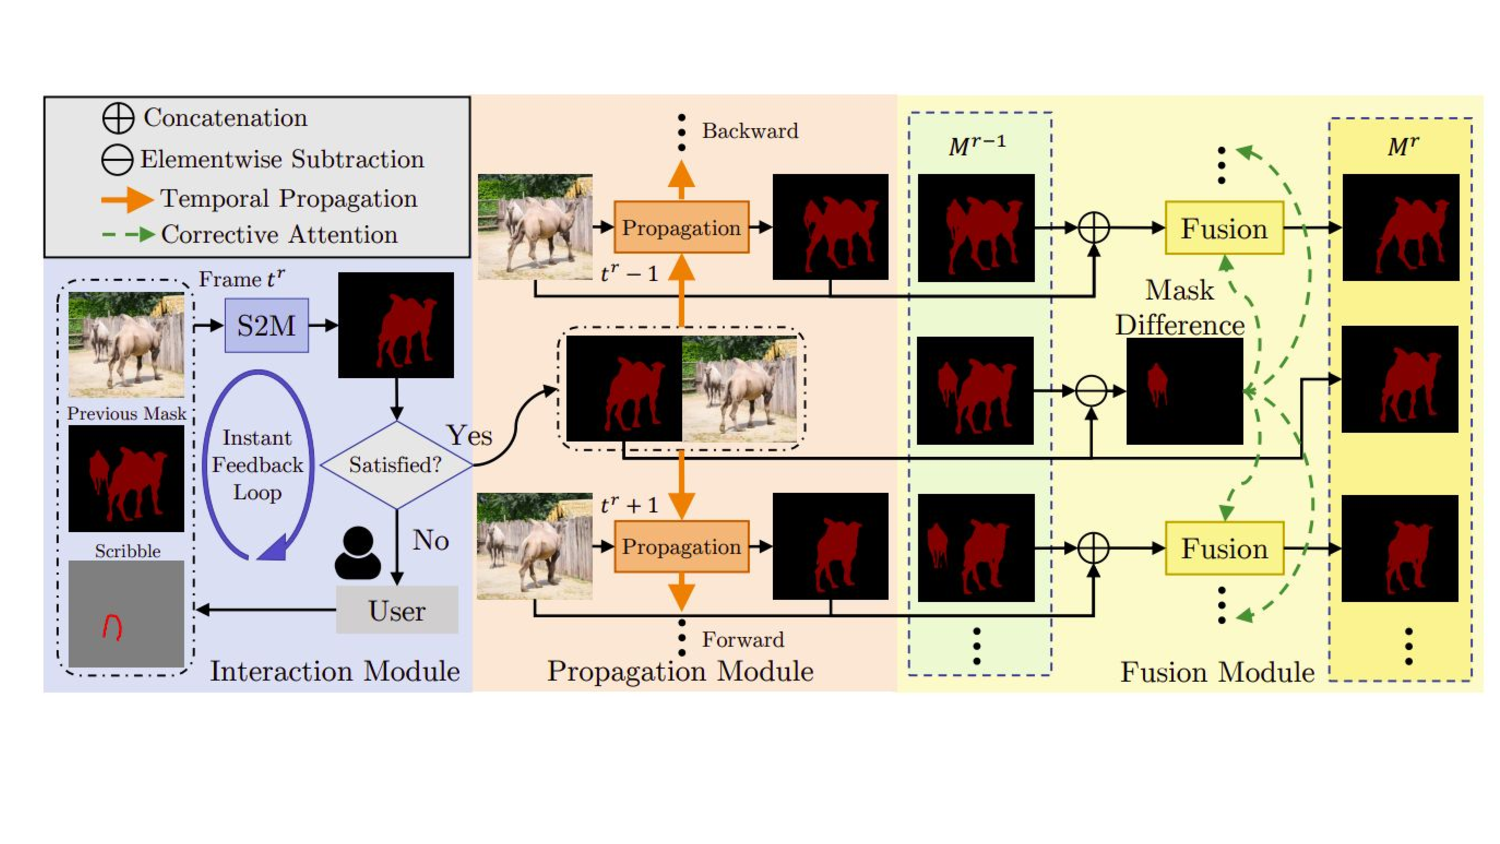
\includegraphics[width=\textwidth]{content/resources/new_images/models/mivos.pdf}
    \caption{Overview architecture of MiVOS \cite{cheng2021mivos}}
    \label{fig:mivos}
\end{figure}

Among these extensions, we adapt STCN \cite{cheng2021stcn} as one of our main modules for refinement as it is simple and effective. but with minor modification. However, most variants cannot handle long videos due to the ever-expanding feature memory bank of STM.

\begin{figure}[!h]
    \centering
    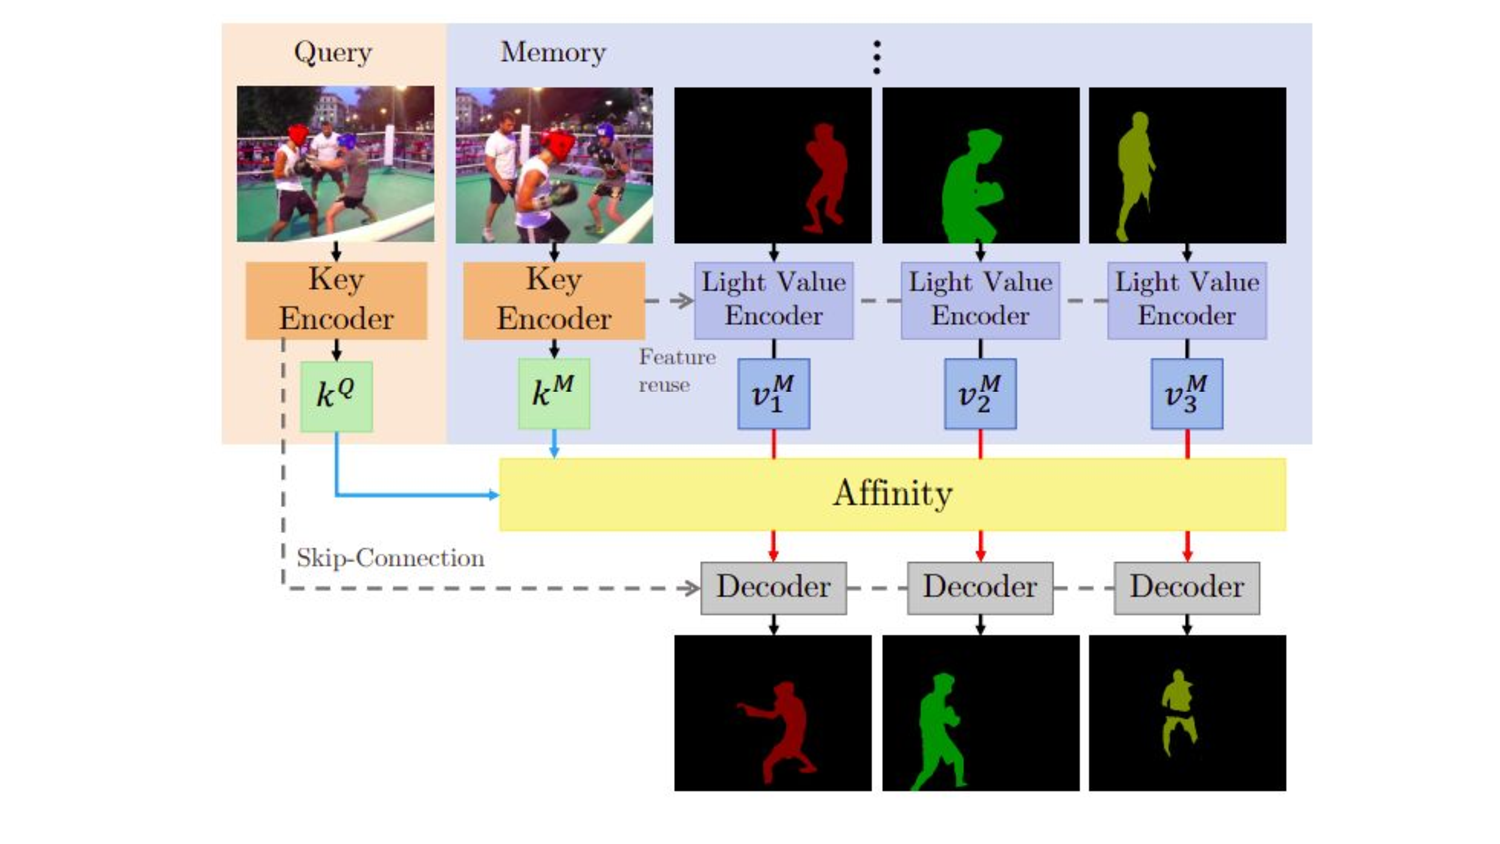
\includegraphics[width=\textwidth]{content/resources/new_images/models/stcn.pdf}
    \caption{Overview architecture of STCN \cite{cheng2021stcn}}
    \label{fig:stcn}
\end{figure}

Nonetheless, the mask propagation and segmentation are still computed individually for different objects. The
problem restricts the application and development of the VOS with multiple targets. Hence,  \cite{yang2022associating} proposes AOT to associate and decode multiple targets simultaneously, as efficiently as processing a single object. Moreover, it is the first method to utilize Transformer modules inside mask-propagation

\begin{figure}[!h]
    \centering
    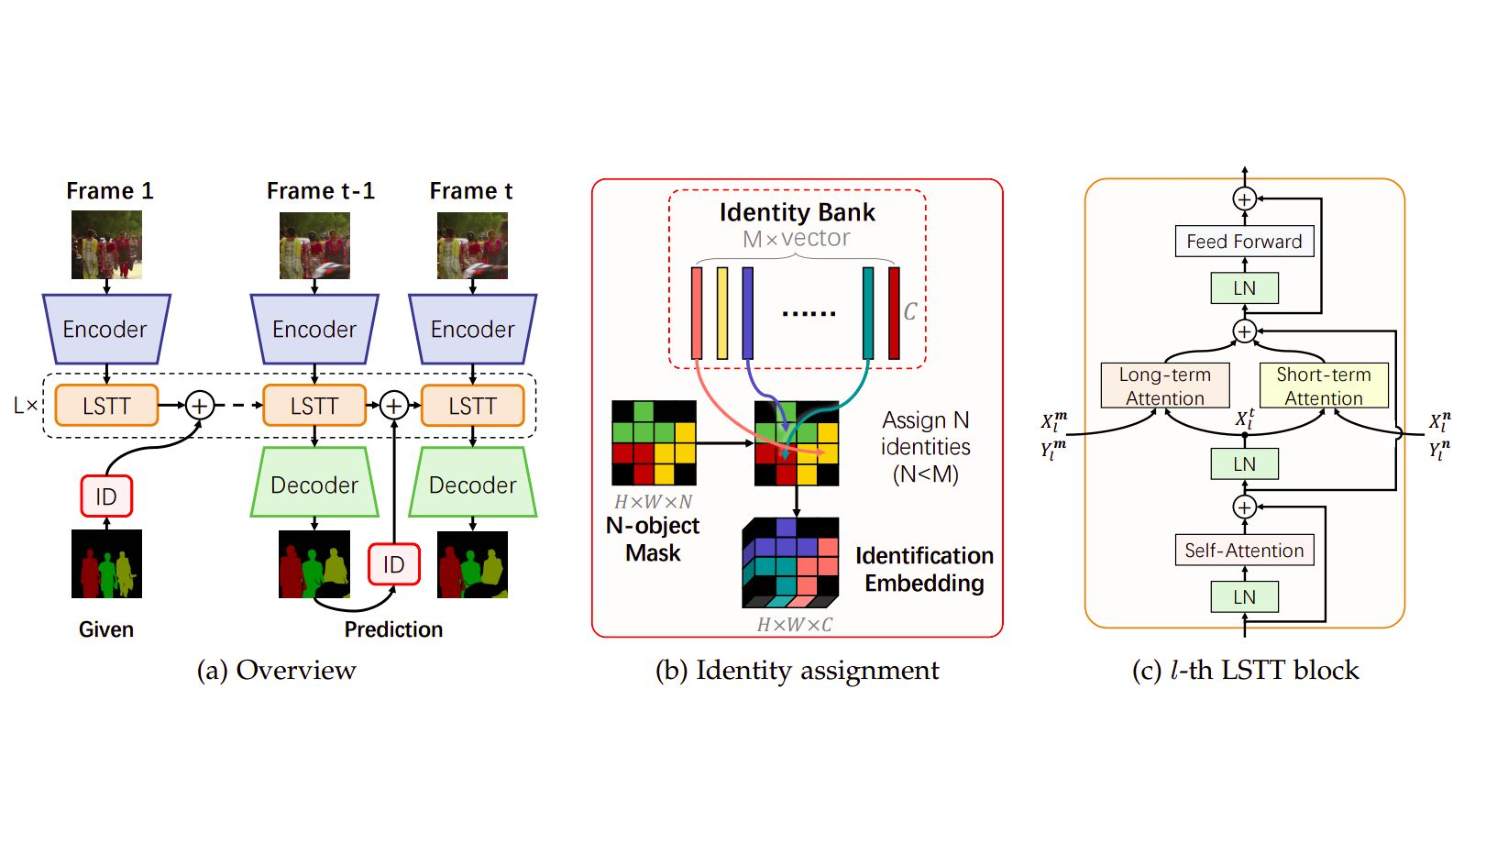
\includegraphics[width=\textwidth]{content/resources/new_images/models/aot.pdf}
    \caption{Overview architecture of AOT \cite{yang2022associating}}
    \label{fig:aot}
\end{figure}

Yet, it still does not solve the GPU memory explosion problem. Recently, authors of STCN \cite{cheng2021stcn}, develop XMem \cite{cheng2022xmem} which uses multiple memory stores to capture different temporal contexts while keeping the GPU memory     usage strictly bounded due to the long-term memory and consolidation.

\begin{figure}[!h]
    \centering
    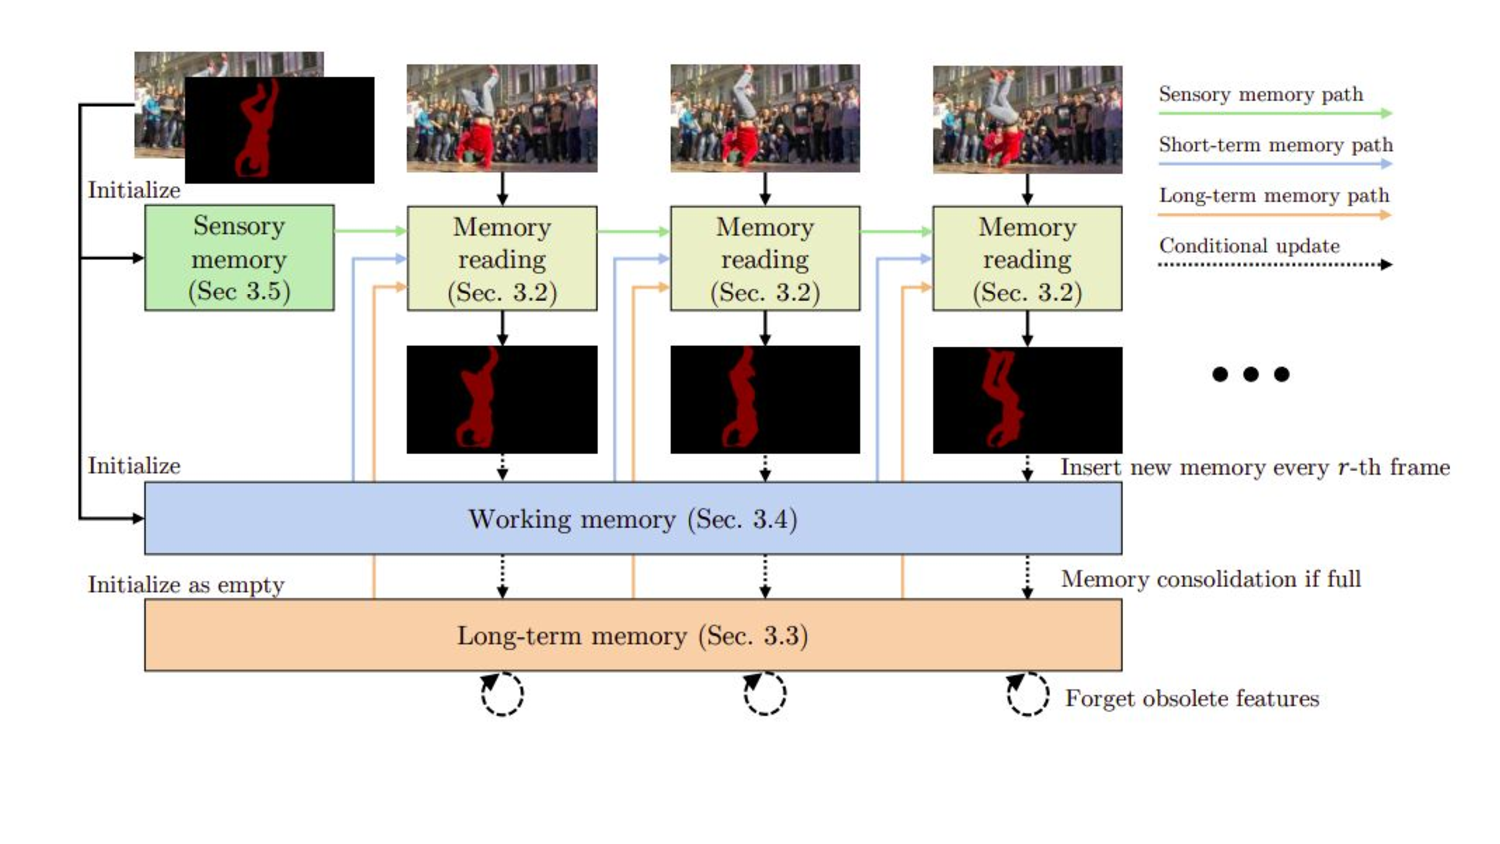
\includegraphics[width=\textwidth]{content/resources/new_images/models/xmem.pdf}
    \caption{Overview architecture of XMem \cite{cheng2022xmem}}
    \label{fig:xmem}
\end{figure}


Although video object segmentation has yielded promising results in a number of domains, these approaches have not been exploited for medical dataset creation. The use of medical images for training and testing machine learning algorithms is critical to the development of accurate models that can be used to diagnose and treat diseases. In order to improve the accuracy and effectiveness of machine learning algorithms for medical image analysis, it is important to develop novel methods specifically tailored for this domain. Mask propagation is a popular technique in interactive scenarios of video object segmentation. 

The user will refine the inputs to the algorithm in order to segment the target objects more accurately. Our proposed concept is heavily inspired by the DAVIS Challenge on Video Object Segmentation. After the first raw prediction of the associate model, the user will interact with some of the valuable slices. After that, they will submit their predicted masks to a server for review. In each of these subsequent interactions, from a list of slices specified by themselves, they choose one frame with an uncertain prediction and provide it to a server who then provides them with a new set of scribbles in this frame which points out regions that are false positives or negatives 




\section{Temporal Position Encoding}
\label{sec:positional_encoding}

After the breakthrough of deep learning in still-image recognition originated with the introduction of the AlexNet model \cite{krizhevsky2012imagenet}, there has been active research devoted to the design of deep networks for a sequence of images. 

Many attempts in the past leverage CNNs trained on images to extract features from the individual frames and then perform temporal integration of such features into a fixed-size descriptor using pooling, high-dimensional feature encoding, or recurrent neural networks. Karpathy et al. \cite{karpathy2014large} presented a thorough study on how to fuse temporal information in CNNs and proposed a “slow fusion” model that extends the connectivity of all convolutional layers in time and computes activations through temporal convolutions in addition to spatial convolutions. Time-series models have also been widely studied in this task to exploit the capabilities of long-term memory features, like LSTM \cite{hochreiter1997long} or GRU \cite{cho2014properties} or most recently, Transformer \cite{vaswani2017attention}. 

However, different from RNN and LSTM, the self-attention inside Transformer cannot capture position information by design. This is critical, considering that the model is otherwise entirely invariant to the sequence order, which is harmful to video encoding.

One common approach is to use position encodings which are combined with input elements to
expose position information to the model. These position encodings can be a deterministic function of position (\cite{sukhbaatar2015end}; \cite{vaswani2017attention}) or learned representations. 
Convolutional neural networks inherently capture relative positions within the kernel size of each convolution. They have been shown to still benefit from position encodings (\cite{gehring2017convolutional}), however.
For the Transformer, which employs neither convolution nor recurrence, incorporating explicit
representations of position information is an especially important consideration since the model is
otherwise entirely invariant to sequence order.

To overcome this issue, \cite{jung2020global} adopts relative position embedding \cite{shaw2018self}, which ensures translation-equivariance property and allows the model to generalize unseen sequence length during training. Empirically, \cite{jung2020global}  confirms that relative position indeed helps to capture the sequential properties of video content, improving the video encoder' performance further.

In our work, we implement a simple way to inject the position information into the feature vector for the model to learn, in the hope that the target model will be capable of understanding relatively the location of specific objects within a long sequence, in our case a CT volume.

In fact, looking at the problem of abdomen organ segmentation in CT volume, this position embedding can be seen as a model constraint since any organ of a human only appear in certain areas. Therefore, with the introduction of this information, the model can comprehend the knowledge of organ relative position to make a better prediction. 

Many previous works manipulate model outputs by incorporating conditions to the model inputs or intermediate features. \cite{mirza2014cgan} first introduce encoding label information into both discriminator and generator to control the generation of the image. \cite{messina2021transformer} also has its own way to concatenate encoded bounding-boxes values to the input vector for the model to learn. All these mentioned research uses only simple embedding layers to embed the scalar values, which encourages us to do the same. 
% \chapter{Proposed Method}
\label{chap-method}
In this chapter, we present our solution for tackle the interactive volume object segmentation. Our proposed approach include reference and propagation module. At first, the pipeline of the method is shown. Then, each module is introduced and the detailed implementation is presented. We apply the distillation technique not only in architecture design but also in the training strategy stage. Finally we dive deep in the potential of loss function especially for medical.

\section{Overview}
\label{sec:overview}

\subsection{A brief introduction to Information Retrieval and the merits of Video-Text Retrieval}
%  paragraph 1
In recent years, we are witnessing impressive growth in both computer hardware and software, which have contributed to the outcomes’ improvement of many expensive tasks, including search.
Information Retrieval (IR), or search in common, is a long-history task claimed to appear in the third century BC in an early type relevant to library administration \cite{eliot2009companion}.
What people know of this terminology today is usually related to electronic devices and the Internet. For example, we may seek a friend’s name in a phonebook or look for a song from its lyrics, a movie from its content by using some search engines.
When we do not know something, instead of going to the library or any kind of information center like we did in the past, most of us constantly “google” it at first.
All of those examples, in fact, are associated with something called Information Retrieval System (IRS) - the implementation of any specific IR theory into the computer operation.
An IR system feeds a query in a particular type as input and gives back the most relevant results to the user through automatic matching methods between the input and data sources (see figure \ref{fig:IR_structure}).
\begin{figure}[!t]
    \centering
    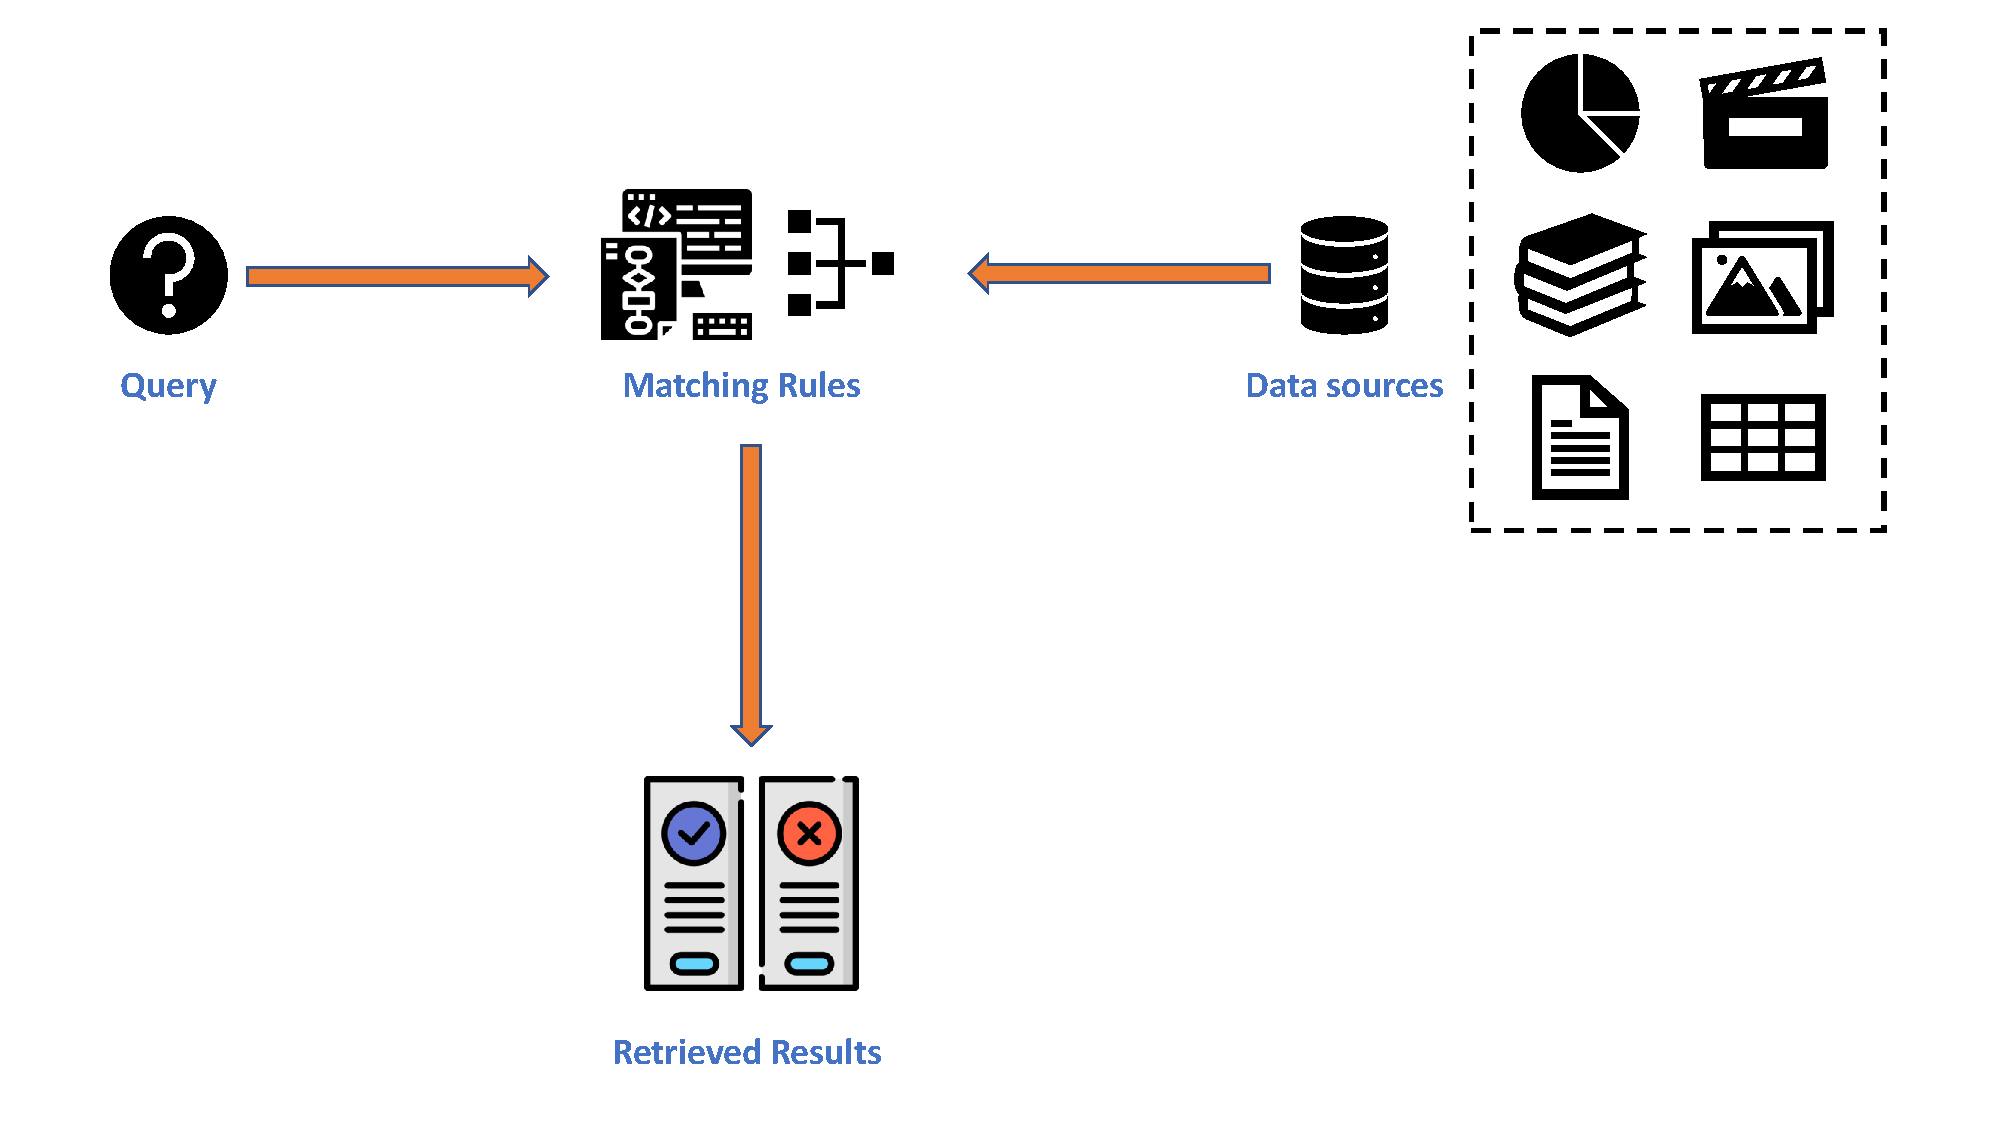
\includegraphics[width=\linewidth]{resources/images/overview/IR_structure.pdf}
    \caption{A simple overview of the Information Retrieval System}
    \label{fig:IR_structure}
\end{figure}
The need for such things occurred due to the increasingly rapid rise in data size and various kinds of information in different areas (like multimedia, website, scientific publication, etc.), making traditional searching techniques no longer cope.
In any IRS, there are always two aspects to deal with: system operation and matching algorithms. Since the first application in the 1940s, it has been developed continuously until now, with many essential milestones \cite{sanderson2012history} tackling both aspects.

%  paragraph 2
As the computing environment changes from time to time, many applications of IR have been suggested, like search on social networks, desktop element search, or one research hotspot recently named cross-modal retrieval.
This task aims to pick out relevant data across different modalities, such as image-text, video-text, audio-text.
Maragos et al. \cite{maragos2008multimodal} stated two future challenges with multimodal applications, including (i) Natural access and high-level interaction with multimedia databases and (ii) Detecting, recognizing and interpreting objects, events and human behavior in multimedia videos by processing combined audio-video-text data.
This statement also reflects two aspects that people always deal with the IRS, as mentioned above.
In research, people may care more about the method aspect than the other.
Traditional methods with manually designed representations, features and matching functions lack the ability to tackle complex IR tasks like multimodal interaction when those tasks require a deeper understanding of document contents and the user information needed \cite{culpepper2018research}.
However, thanks to an ever-stronger influence of Deep Learning \cite{goodfellow2016deep,lecun2015deep} in the 2010s decade, many problems raised in this field have resulted in better performance, letting people expect a new generation of robust and intelligent cross-modal Information Retrieval Systems.

%  paragraph 3
Also, humans have recently witnessed a rapid explosion in the appearance of videos in many aspects of their daily lives.
We all know the potential of videos in entertainment, communication, data analysis, etc.
The rise of video-based online services like YouTube, Netflix, along with the traditional TV program, has inspired Computer Vision (CV) experts to pay more attention to this resource. Additionally, natural language (NL) is one of the most effective means to describe those video contents.
From this point of view, the task of searching videos via text queries, or video-text retrieval, in short, becomes a desirable function in intelligent systems.
This problem takes (a) natural language text description(s) as input and outputs a sorted list of videos in terms of semantic relevance.
A lot of neuron network-based methods, focusing on transforming text input and video’s particular contents into the same subspace and measuring their similarity, have worked efficiently.
However, each video retrieval task has its own specificities among the diversity of the visual world, besides some in-tackling challenges like the semantic gap between two modalities, lack of annotated video-caption, or complicated consideration of temporal information, making no universal utilization approach fit for all such retrieval problems.
Therefore, caption-to-video retrieval is still attracting researchers to resolve in different areas.

\subsection{A brief introduction to Intelligent Transportation/Traffic System and the merits of Vehicle-oriented Computer Vision Tasks}
%  paragraph 1
Transportation is a non-separable part of any country, playing an essential role in different aspects of our daily life.
Residents, governments, and businesses almost depend on it to access resources.
Therefore, the advent of Intelligent Transportation/Traffic System (ITS), a significant factor contributing to the concept of smart city and to the development of modern civilization, is inevitable.
The implementation of ITS is widely accepted and used in many countries today when the governments recognize (i) the rapid growth of the human population, (ii) high-speed urbanization, and (iii) increasing vehicle ownership.
Though there are multiple modes of transportation, the roadway is the most common route.
So this kind of system aims to address a wide range of road traffic issues via advanced technologies, solving at three main levels: society, the road administrator, and drivers.
By providing different modules centering around the people-vehicle-road relation, and other traffic objects, it helps improve the safety, efficiency,  and environmental friendliness of the transportation.

%  paragraph 2
In an ITS that inherits Deep Learning works, Fan et al. \cite{fan2020deep} have shown that there are four major services in the architecture, as illustrated in figure \ref{fig:ITS_structure}.
\begin{figure}[!t]
    \centering
    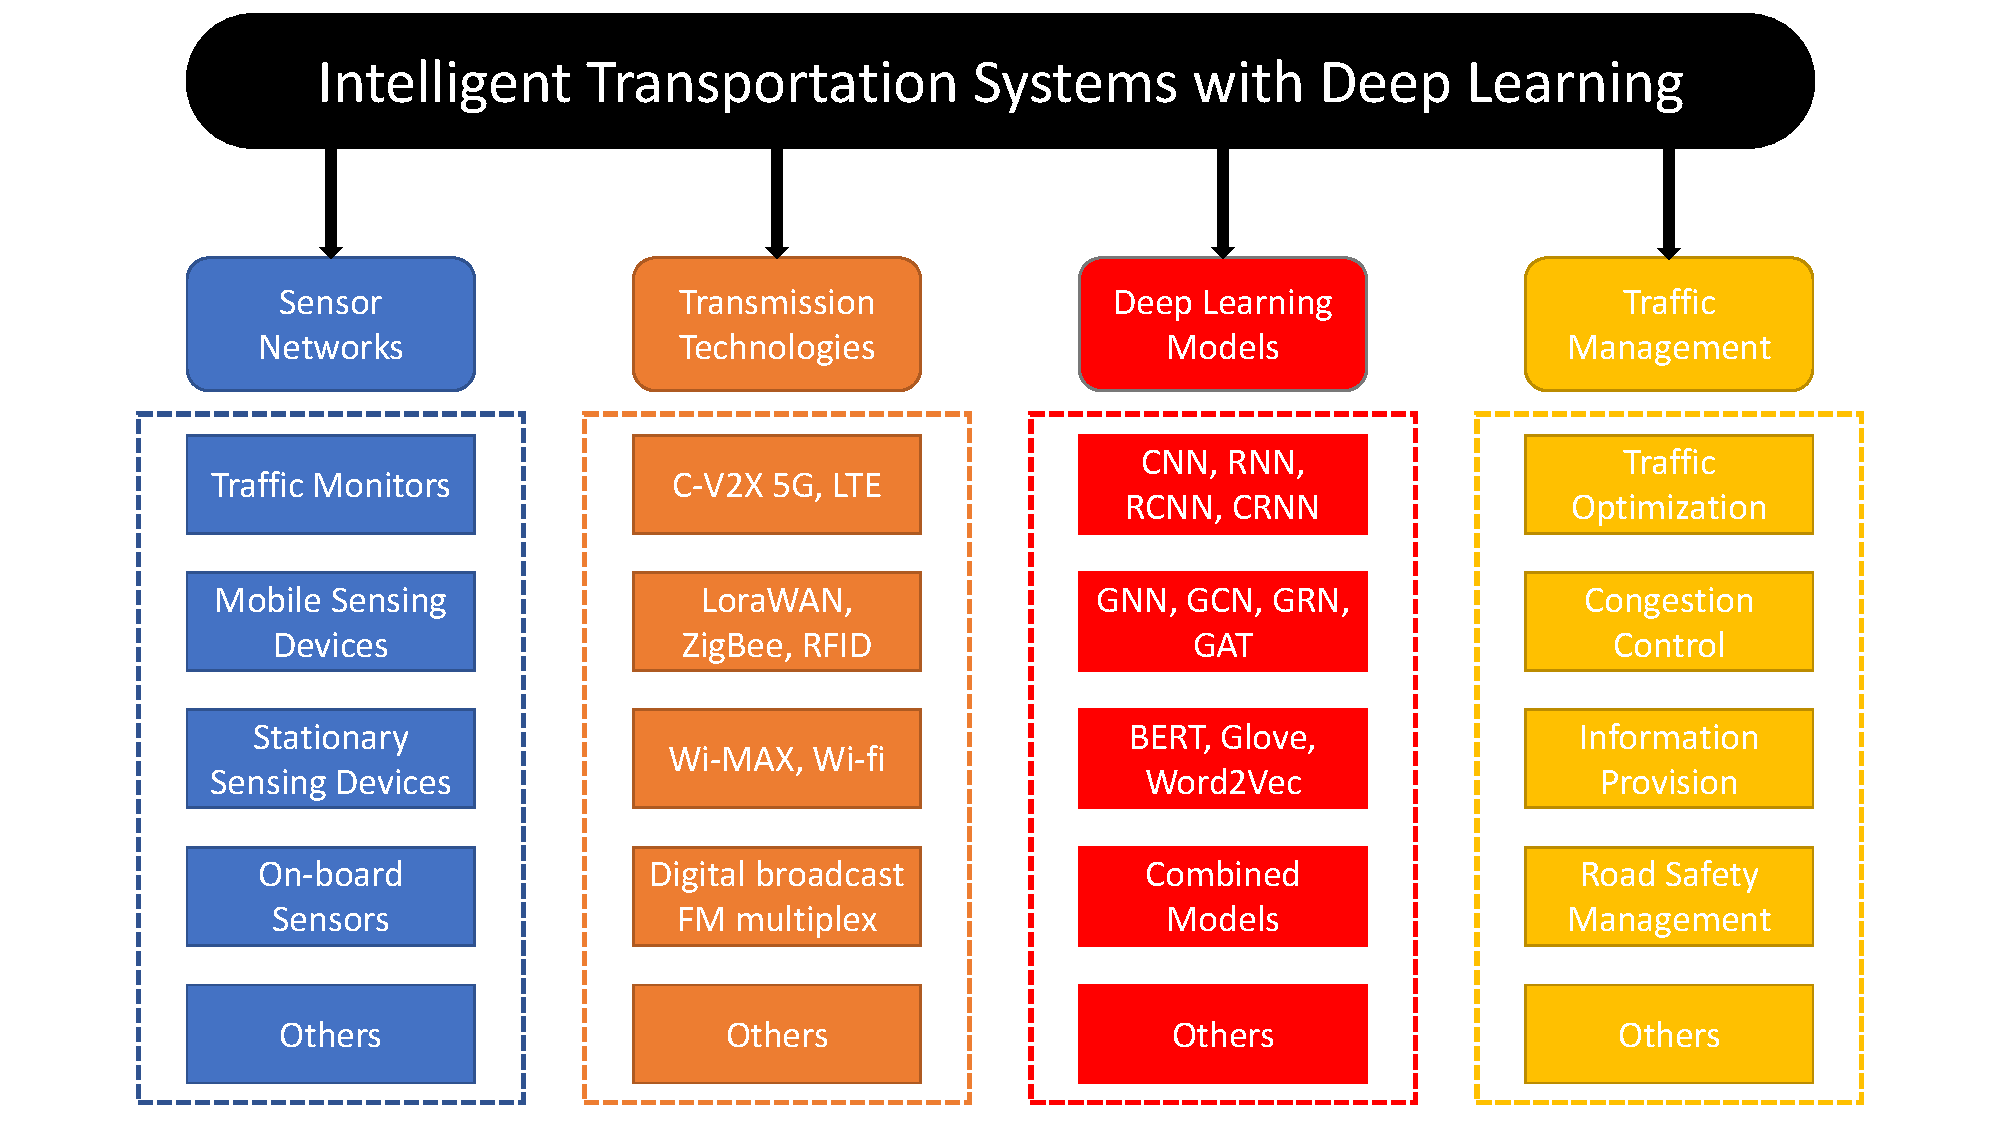
\includegraphics[width=\linewidth]{resources/images/overview/ITS_structure.pdf}
    \caption{Major components of a Deep Learning-based Intelligent Transportation/Traffic System.}
    \label{fig:ITS_structure}
\end{figure}
The Sensor Networks service is in charge of collecting real-time data then sends it through the Transmission Technologies service.
By exploiting the data, the Deep Learning Models service is responsible for building models that can perform well in particular tasks before integrating them into practical modules of the Traffic Management service.
When it comes to Computer Vision applications in such systems, many problems are mainly related to vehicles.
This is because transportation is vehicle-centered, unlike other areas, which are often people-focused.
Thanks to the widespread installment of 24/7 surveillance cameras on roads and highways, people can obtain massive traffic data.
Although the potential for video analytics from that data is enormous to be leveraged, it has not been exploited optimally.
Some tasks have received high-accurate state-of-the-art results, such as Vehicle Counting \cite{lu2021robust, dai2019video, asha2018vehicle} or Vehicle Reidentification \cite{luo2021empirical, Khorramshahi_2019_ICCV, zhu2019vehicle}, but some are still far from saturated outcomes.
Two major hurdles include the insufficiency of labels and the lack of high-performance models capable of converting data into valuable insights.
Regarding the model, since the vehicle is a particular domain and non-human, many pre-trained models cannot be applied directly to this object.
Therefore, CV researchers in this field still face so many significant challenges.
And, there should be something that can attract attention to address such issues.

%  paragraph 3
For those reasons, in parallel with the works of individuals, there are also organizations holding vehicle-oriented contests in order to find solutions from talented candidates.
Not stopping there, through these contests, people hope for deployments of submitted models into a realistic environment. 
One of the hottest contests is the AI City Challenge \cite{Naphade17AIC17, Naphade18AIC18, Naphade19AIC19, Naphade20AIC20, Naphade21AIC21}, opening continuously since 2017.
This contest primarily focuses on accurate, robust, and efficient approaches, so the organizers provide relatively sufficient labeled datasets \cite{Feng21CityFlowNL, Tang19CityFlow, Yao20VehicleX} as well as the evaluation system.
Their problems range from the mentioned tasks above to others like Velocity Estimation, Anomaly Detection, Vehicle Tracking, etc., whose insights may be inspired by various techniques.
In the latest edition, the 5th AI City Challenge \cite{Naphade21AIC21} has proposed a novel advanced track named Natural Language-Based Vehicle Retrieval (NL-based VR), which needs an effective combination of subtasks including motion detection, appearance recognition and content-based video retrieval.
There are still other tasks from other competitions, but finally, they all have the same goal: to solve real-world traffic issues and implement them into the Intelligent Transportation/Traffic System.
\section{Preprocessing}
\label{sec:preprocess}
For preprocessing, we apply Windowing technique  \cite{windowingct17yahya} with different levels and widths to target specific parts of human organs. Windowing, also known as grey-level mapping, contrast stretching, histogram modification or contrast enhancement is the process in which the CT image grayscale component of an image is manipulated via the CT numbers; doing this will change the appearance of the picture to highlight particular structures. The brightness of the image is adjusted via the window level, window level determines the central or midpoint grey value for the range of HU displayed in the image. Ideal imaging of different tissues depends on the window level. The contrast is adjusted via the window width. A wide window (400-2000 HU) is suitable for examining structures of vastly different attenuation values. For instance, chest structures are best viewed using a wide window.

In or experiments, we apply 3 wide windows corresponding with 3 different versions of a single slice by highlight the abdomen, chest, and spine groups and stack it to one as a three-channel image (Fig. \ref{fig:windowingct}). The window parameters in our experiments are shown in table \ref{table:window_params}
\begin{table}[]
\centering
\caption{Window parameters}\label{table:window_params}
\begin{tabular}{| l | c c |}
\hline
Group      & Window level & Window width \\ \hline
Spine-bone & 900          & 1400         \\ \hline
Tissues    & 200          & 350          \\ \hline
Chest      & 787          & 2137         \\ \hline
\end{tabular}
\end{table}

Where the group of the soft tissue masses can be determined by merging of the abdomen soft tissues and liver. The chest group, which consists of the lungs and mediastinum. By re-calculating the window information from the min value and max value of selected range, these window parameters can be accurately determined.

\begin{figure}[!h]
    \centering
    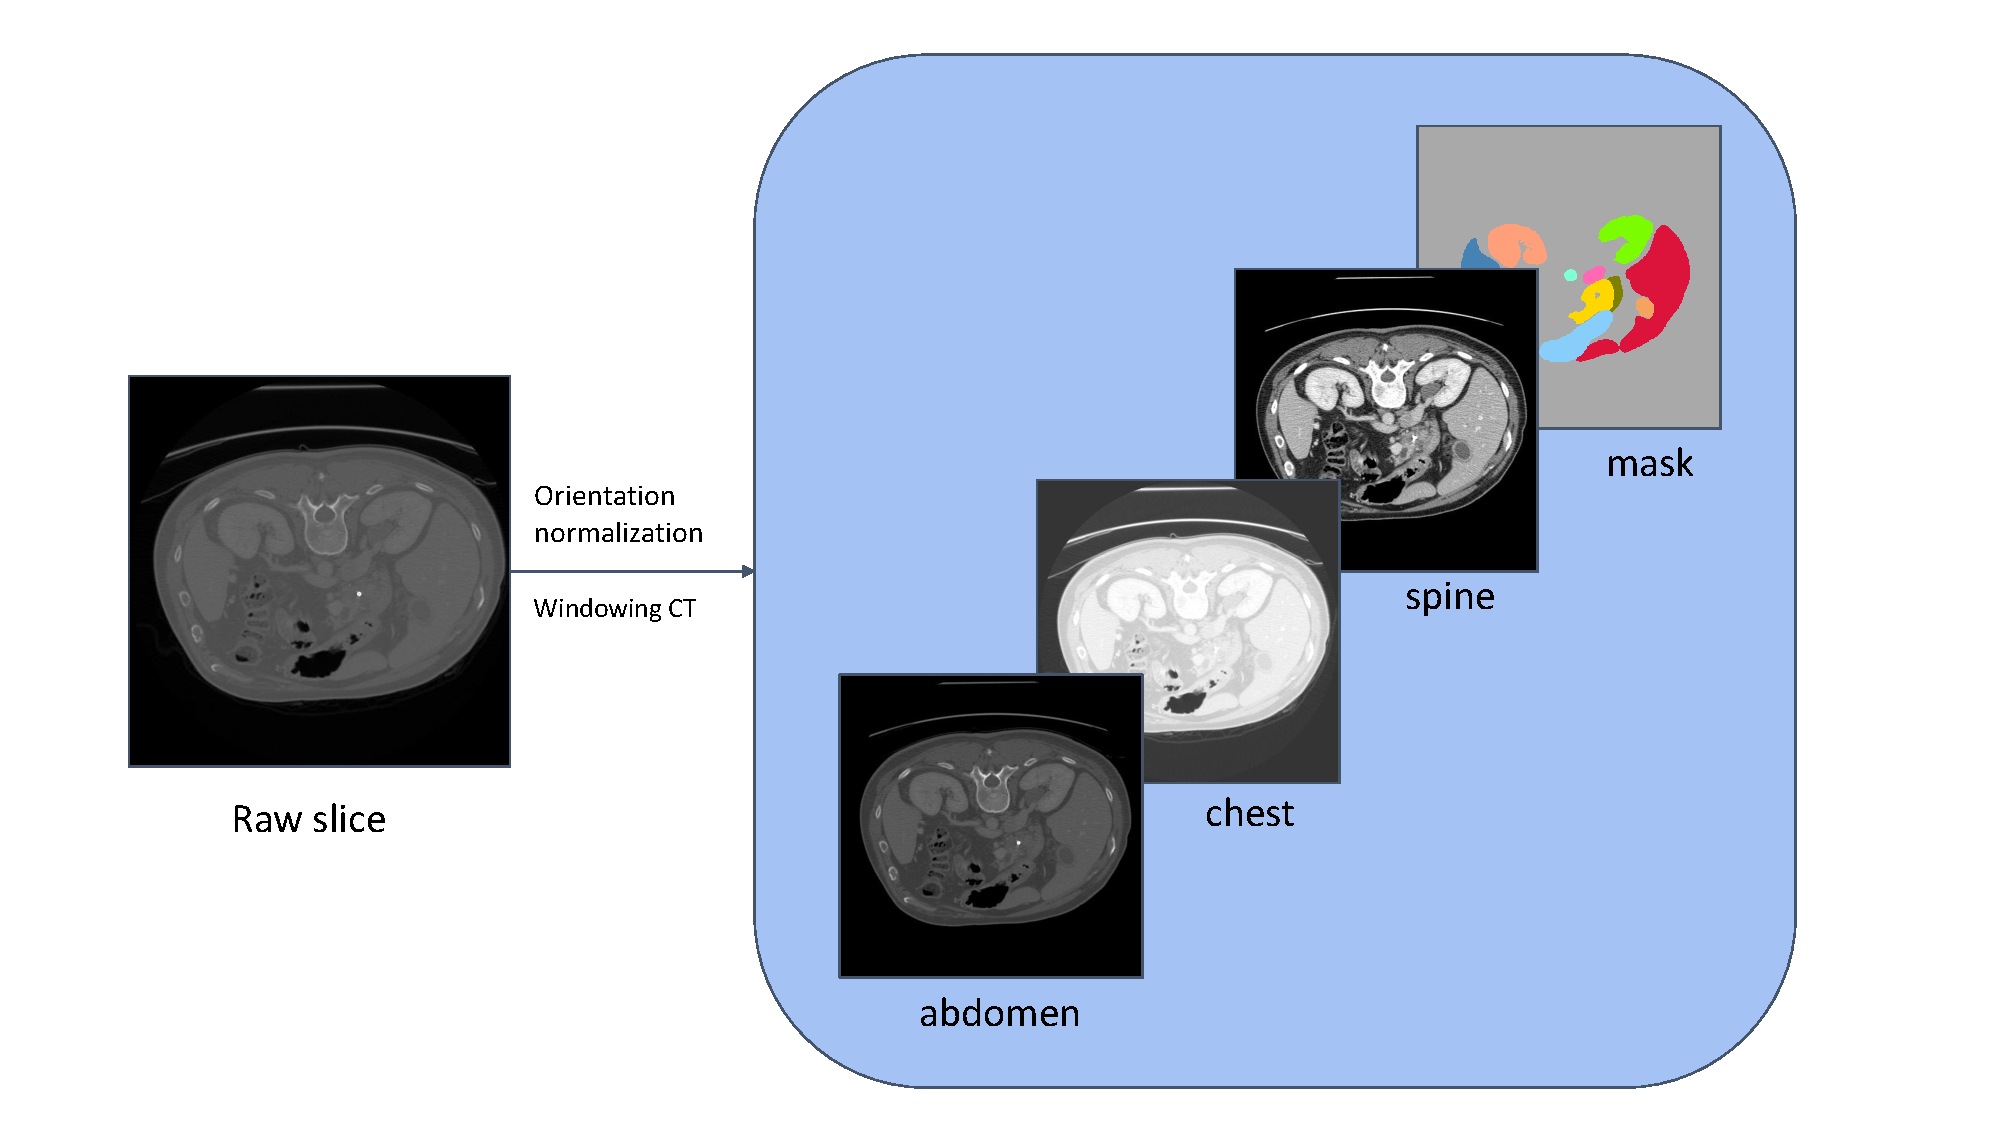
\includegraphics[width=\textwidth]{resources/new_images/preproc.pdf}
    \caption{Windowing CT. 3 different versions are generated from an original slice. }
    \label{fig:windowingct}
\end{figure}

In addition, we choose the axial plane to cut the slices from the CT volumes since this plane has various dimension sizes. 
Due to some relatively small organs, it might be better to keep the original size of the slices without any cropping, resampling, or resizing methods.
The image is rotated to a predefined angle, then divided by 255 for normalization before going through the next step.
\pagebreak
\section{Reference module}
\label{sec:reference}
\begin{figure}[!htb]
    \centering
    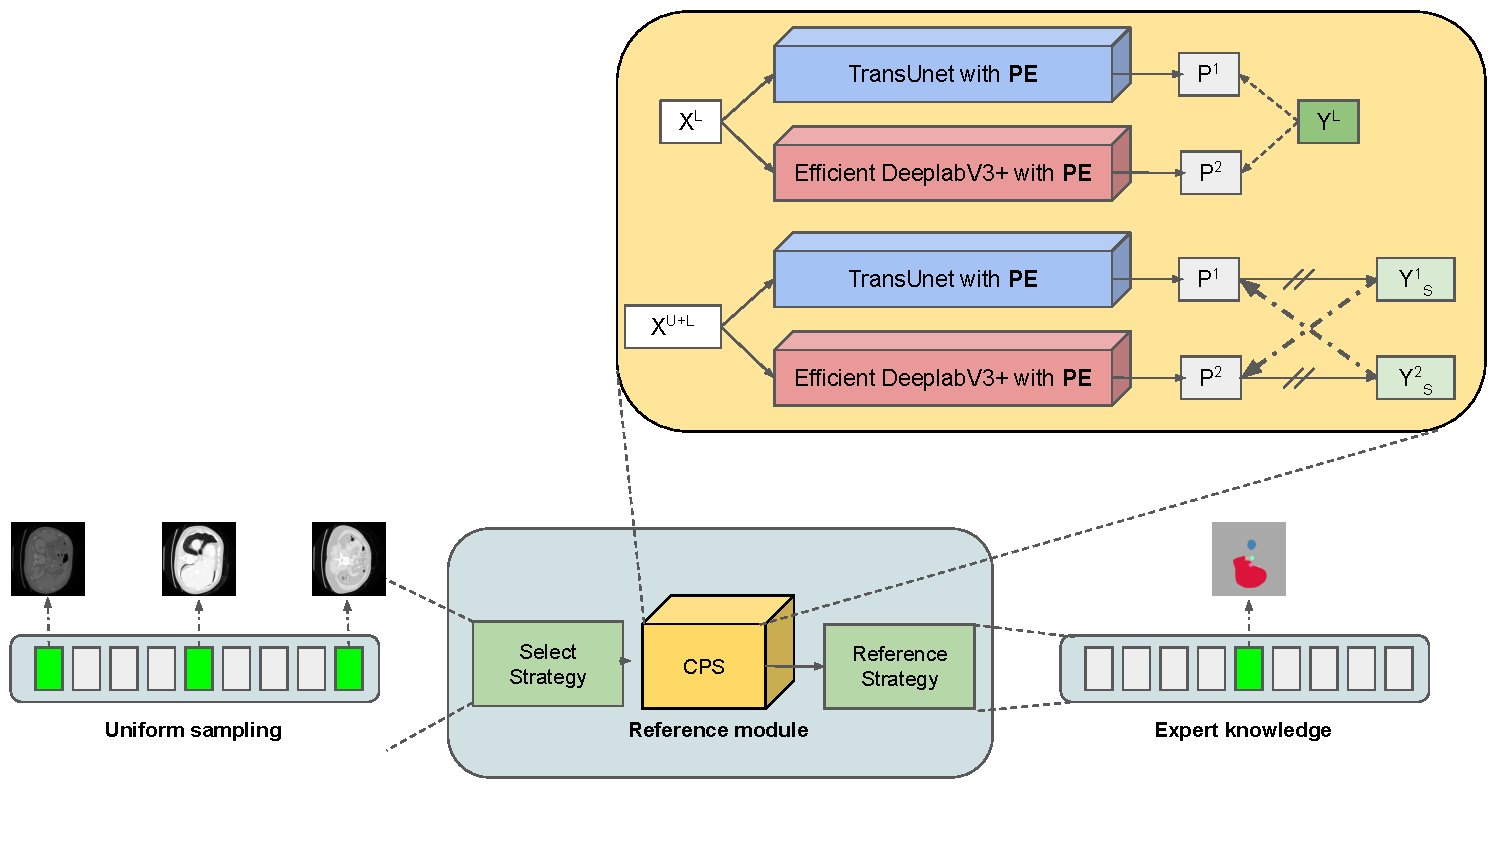
\includegraphics[width=\textwidth]{content/resources/new_images/reference.pdf}
    \caption{The reference module. The semi-supervised technique CPS is applied in both training and inference stage to enhance the precision of model prediction. Strategies are used to smartly choose slices that are informative for the next stage. }
    \label{fig:reference}
\end{figure}


This module is expected to provide a suggestion of a minimal amount of slices and predicted masks that might contain the most information describing the entire CT Volume. Fig \ref{fig:reference} describes the details of this module.

To utilize the enormous number of unlabeled data, we apply the recent semi-supervised method that performs effectively on several other datasets, which is called Cross Pseudo Supervision (CPS) \cite{cps21chen} (yellow cube in Fig. \ref{fig:reference}).
CPS enables the usage of unlabeled data by following the dual students technique, where two models are trained simultaneously on labeled data while generating pseudo data for their "peer" to learn. In the testing phase, two models predict the same image, and the result is aggregated by summing up.

We adopt two prominent state-of-the-arts 2D segmentation models with highly different learning paradigms for this CPS framework, which is TransUNet \cite{transunet21chen} and DeeplabV3+ \cite{dlv3p18chen}. While DeeplabV3+ traditionally focuses more on the local information, transformers model the long-range relation, so the cross training can help to learn a unified segmenter with these two properties at the same time. In short, we choose TransUNet and DeeplabV3+ due to their ability to compensate each other for better performance. \cite{crosscnntransformer21luo}


% Transformers are a novel architecture that solves sequence to sequence tasks while handling long-range dependencies. Transformers are used standalone or combined with CNN(Convolutional Neural Networks), significantly boosting computer vision tasks

In addition, we also propose a both logical and specialist-based strategy to choose which slices can be further used to boost the performance of the Propagation module. The goal of this action is to preserve only some of the most useful information for the refinement stage.

To elaborate on these strategies, prior to being put into the CPS module for prediction, a small number of slices are uniformly sampled from the processed CT volume. After CPS produces segmentation masks for these slices, another selection step is performed to pick only some of the masks that contain the organs having the largest areas.  
\section{Propagation module}
\label{sec:propagation}
\begin{figure}[!h]
    \centering
    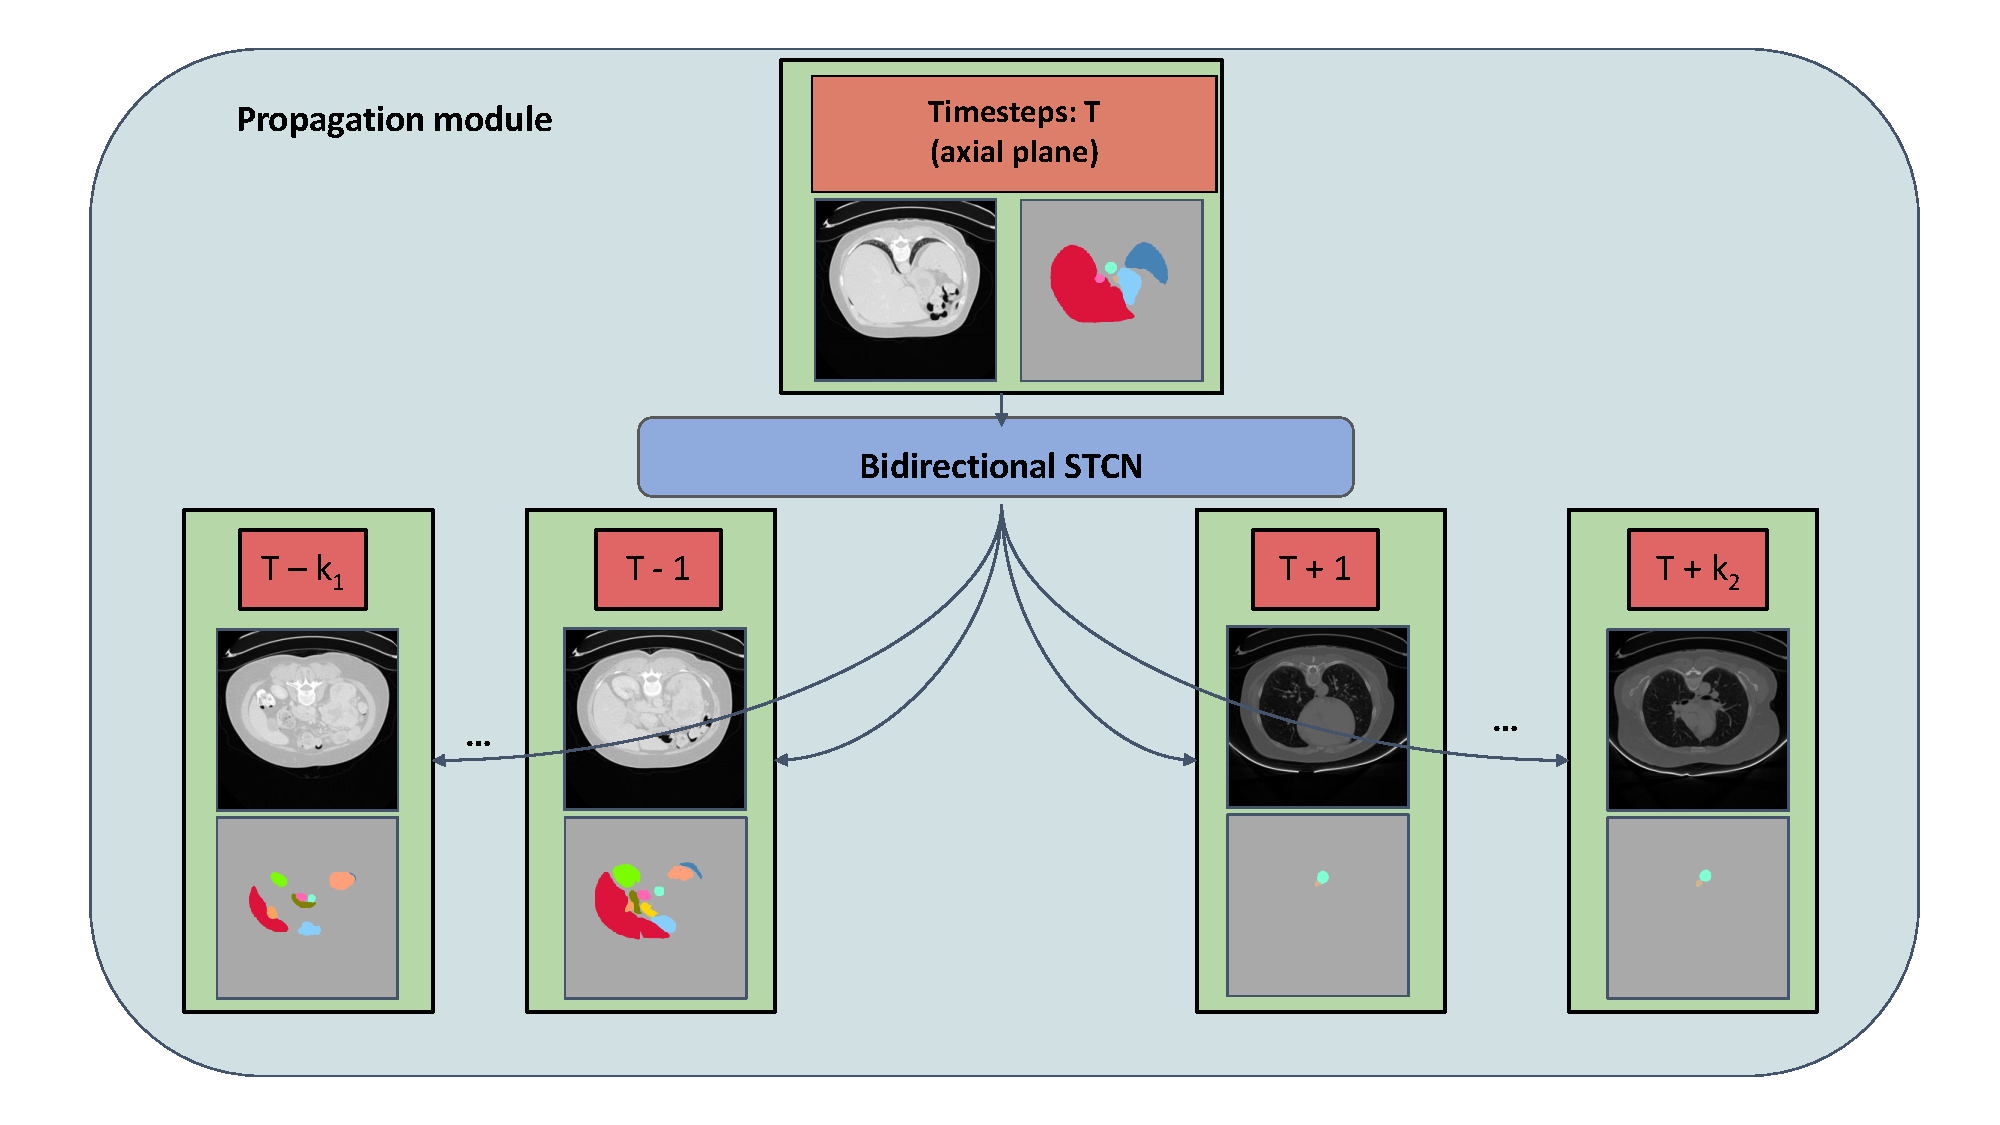
\includegraphics[width=\textwidth]{content/resources/new_images/propagation.pdf}
    \caption{The propagation module. From an annotated slice of CT, at timestep T, STCN can make use of that to spread the information through the entire defined range $[T-k_1, T+k_2]$.}
    \label{fig:propagation}
\end{figure}

This module aims to utilize prior knowledge of given annotated slices from the Reference module to make prediction on the remaining slices, this mechanism can be referred as mask (or label) propagation.

Intuitively, the conventional 2D CNNs cannot comprehend the third dimension information within a CT volume. Thus, in hope of the ability to capture the "temporal" information along the axial plane, we adapt the Space-Time Correspondence Networks (STCN) \cite{stcn21cheng}, which is a semi-supervised segmentation algorithm that has achieved promising results on Video object segmentation problem, to this 3D manner. 

Basically, STCN proposes the use of a memory bank that stores information about previous frames and their corresponding masks and uses them later as prior knowledge. To generate the mask for the current frame, a pairwise affinity matrix is calculated between the query frame and memory frames based on negative squared Euclidean distance, then it is used for supporting the current mask generation \cite{stcn21cheng}. 

Different from the original STCN, we slightly modify it to match the current problem. In the original work, they use only a single dense mask to propagate through the entire video, therefore for the model to perfectly work, that selected mask must contain information about all available classes. For our case to achieve that, we enable the usage of multiple masks for propagation, so that all of these masks should contain enough information about every organs. We also allow the STCN to work in a bidirectional way to enhance the refinement. Fig \ref{fig:propagation} illustrates this process.

Specially, STCN can be simply trained in the binary manner, meaning that each of the abdominal organs can be learned separately. Therefore, the knowledge can be transferred well between different organ classes.
\section{Pseudo Labeling}
\label{sec:labeling}
% \begin{figure}[!htb]
%     \centering
%     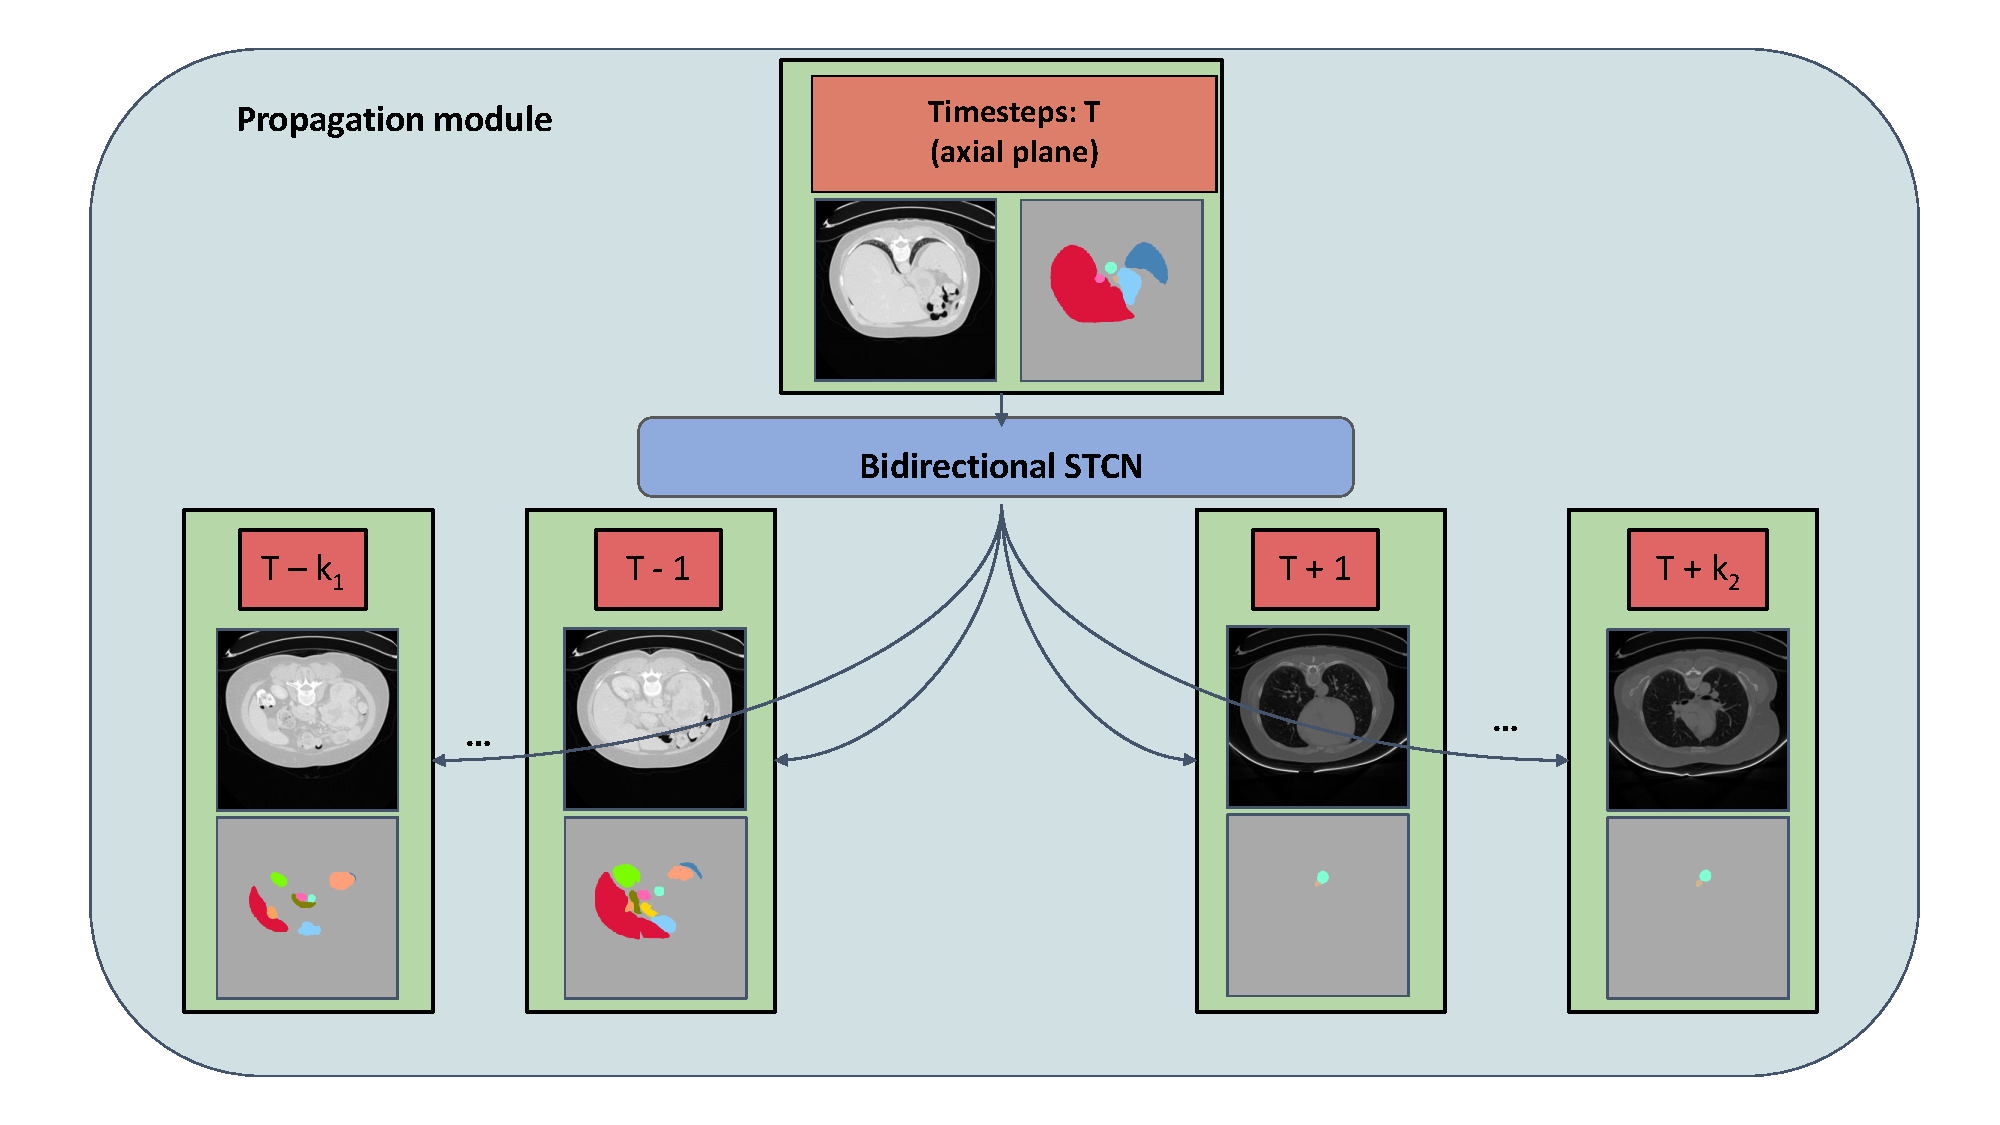
\includegraphics[width=\textwidth]{content/resources/new_images/propagation.pdf}
%     \caption{The propagation module. From an annotated slice of CT, at timestep T, STCN can make use of that to spread the information through the entire defined range $[T-k_1, T+k_2]$.}
%     \label{fig:labeling}
% \end{figure}


Given a vast amount of unlabeled CT volumes, we apply a uncertainty estimation technique to effectively maximize the utilization of the data.

Firstly, several CPS models are trained on the provided labeled data.
Then, we use these trained CPS models to obtain pseudo masks on the unlabeled set. Inspired from \cite{wang2019active}, we calculate the dice scores between these pseudo masks and the aggregated one. The mean of these dice scores will be compared with a threshold to determine whether the aggregated pseudo masks are qualified. Simply speaking, consensus-based assessment is used to evaluate the quality of pseudo labels.

We determine a single score for the $i^{th}$ volume in the unlabeled set as the formulation below:

\begin{align}
        score_{i} &= \frac{1}{K \times M} \sum_{k=1}^{K^{i}} \sum_{m=1}^{M} \text{DSC}(\mathcal{Y}^{k,i}_{m}, \mathcal{Y}^{k,i}_{AVG}) \\
        \text{dsc}  &= \frac{2 |X \cap Y|}{|X| + |Y|}
\end{align}

DSC represents the Dice Score evaluation metric calculating the overlapping area of prediction $X$ and ground truth $Y$. 
Here $\mathcal{Y}^{k,i}_{m}$ indicates the $m^{th}$ model’s output of the $k^{th}$ slice of volume $i$ while $\mathcal{Y}^{k,i}_{AVG}$ is the mask averaged from all $M$ models for the same slice. The easier the sample is, the more inclined the segmentation are to get a similar output if the sample is easier. In contrast, hard samples are more likely to be segmented differently by different models. Hence, we use the proposed score to measure the certainty between models' predictions. Higher score gives more credibility to the prediction, as it is more consistent. 

All aggregated samples that have high certainty are then reused for the next supervised training cycle. And after the training finishes, the same labeling process is repeated until all aforementioned models achieve satisfied performance or every unlabeled data has been used.
\section{Loss functions}
\label{sec:loss}

For the Reference module, we use the prevalent combination of dice loss and cross entropy loss with smoothing value to alleviate the imbalanced number of the small organs, which occurs due to our splitting into slices process. The same settings are used for CPS in its supervised branch whereas only the dice loss is setup for the unsupervised branch. 

For the Propagation module, we implement the online hard example cross entropy (OhemCE or Bootstrapping CE) \cite{ohemce16wu} and also calculate the Lovasz loss \cite{lovasz18berman} at the same time. OhemCE can help reduce the contribution of background label to the final loss. And since STCN is trained on binary task, OhemCE can direct the model to focus on visible difficult objects. Meanwhile, Lovasz loss is commonly used in the past. 


Given y the ground truth mask, and \hat{y} the predicted mask of the model, we reformulate all the losses that we have used in training our networks as below: 

\textbf{Dice loss}

The Dice coefficient is widely used metric in computer vision community to calculate the similarity between two matrices. In recent years, it has also been adapted as loss function known as Dice Loss \cite{sudre2017diceloss}

\begin{align}
        DL (y, \hat{y}) &= 1 - \frac{2\hat{y}y+\epsilon}{\hat{y}+y+\epsilon}
\end{align}

Here, $\epsilon$ is added in both numerator and denominator to ensure that the function is not undefined in edge case scenarios such as when $\hat{y} = y = 0$.

\textbf{Cross-entropy loss}

Cross-entropy is a traditional loss function that is widely used for classification objective, and as segmentation is pixel level classification it works well. It is defined in \cite{yi2004ce} as a measure of the difference between two probability distributions for a given random variable or set of events.
Binary Cross-Entropy is defined as:

\begin{align}
        L_{BCE} (y, \hat{y}) &= -(y log (\hat{y}) + (1-y)log(1-\hat{y}))
\end{align}

\textbf{Online hard example cross-entropy loss}

We et. al \cite{ohemce16wu} propose an online bootstrapping method, which forces networks to focus on hard (and so more valuable) pixels during training. 

Let there be $K$ different categories $c_j$ in a label space. For simplicity, suppose that there is only one image crop per mini-batch, and let there be N pixels $a_i$ to predict in this crop. Let $y_i$ denotes the ground truth label of pixel $a_i$
, and $p_{ij}$ denotes the predicted probability of
pixel $a_i$ belonging to category $c_j$ . Then, the loss function can be defined as

\begin{align}
        L_{OhemCE} &= - \frac{1}{\sum_{i}^{N} \sum_{j}^{K} 1 \{y_i = j \text{ and } p_{ij} < t\}} (\sum_{i}^{N} \sum_{j}^{K} 1 \{y_i = j \text{ and } p_{ij} < t\} log p_{ij})
\end{align}

where t ∈ (0, 1] is a threshold. Here 1{·} equals one when the condition inside holds, and otherwise equals zero. In practice, there should be a reasonable number of pixels kept per mini-batch. Hence, the threshold $t$ will be increased accordingly if the current model performs pretty well on a specific mini-batch.

\textbf{Lovasz-Softmax loss}

 Berman et. al \cite{lovasz18berman} incorporates the softmax operation in the Lovasz extension. Having the similar target as the Dice Loss, The Lovasz extension is a means by which we can achieve direct optimization of the mean intersection-over-union loss in neural networks. In this respect, the Lovasz-Softmax loss can be formulated as follows:
 
 \begin{align}
        L_{lovasz} &= \frac{1}{|C|} \sum_{c \in C} \overline{\Delta_{J_c}} (m(c)) \\
        m_i(c) &= \begin{cases}
                        1 - x_i(c)  & \text{if } c = y_i(c) \\
                        x_i(c)    & \text{otherwise}
                    \end{cases}
\end{align}

where $|C|$ represents the class number, $\Delta_{J_c}$ defines the Lovasz extension of the Jaccard index, $x_i(c) \in [0,1]$ and $y_i (c) \in \{-1,1\}$ hold the predicted probability and ground truth label of pixel $i$ for class $c$, respectively.


% \section{Textual Attribute Extraction}
\label{sec:text_extraction}
\begin{figure}[!htb]
    \centering
    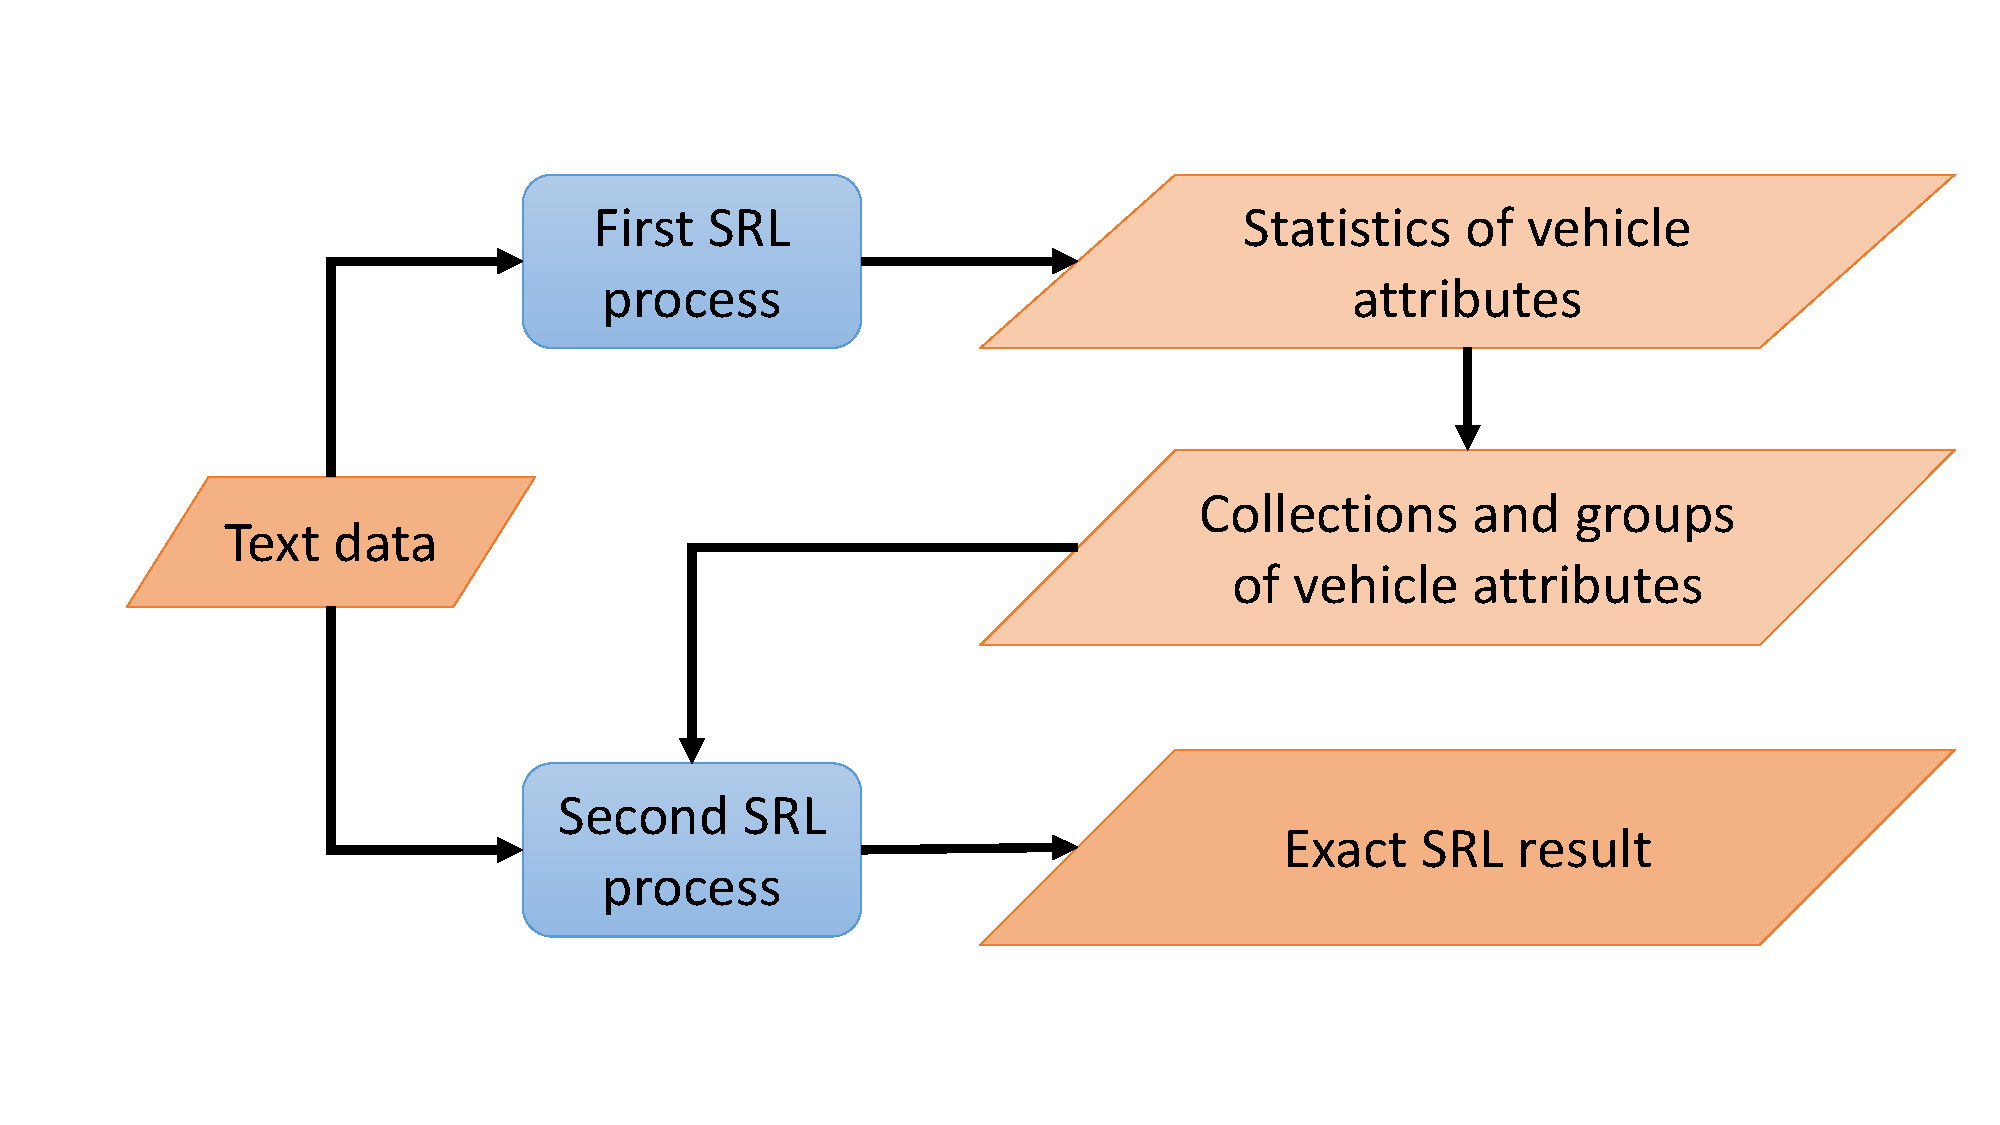
\includegraphics[width=\textwidth]{images/methods/text_branch_overview.pdf}
    \caption{The overview of process flow on text branch.}
    \label{fig:text_branch_overview}
\end{figure}
On such retrieval problems, the text data usually contains rich information about the objects and their activities. Also, this dataset mainly focuses on traffic and vehicle, narrowing the scope of vocabularies but still providing essential information. Therefore, besides feeding the text query into the next-step model, we employ a method to obtain specific query keywords to construct a special collection of vehicle attributes. This task helps us label each query on some categories, useful for later tasks about classification, detector, or re-ranking.
It should be noticed that most of the queries are structured as follow:

\textbf{Vehicle + Action + Optional object(s) + Other information.}

That is the reason we consider English PropBank Semantic Role Labeling (SRL), via the method proposed in \cite{shi2019simple}, as a possibly efficient means to parse verb and noun phrases. A two-phase flow describing the text-branch process is shown in Figure \ref{fig:text_branch_overview}.
\begin{itemize}
    \item First, to analyze the data, we take an SRL extraction on raw data to make statistics on the vehicle's attributes. This process helps us confirm that it is necessary to define potential values about the vehicle types, actions, colors. After filtering the top most frequent and suitable words on each attribute and observing the relation among queries in a track, we create certain groups for three types of the attribute. Figure \ref{fig:group_example} illustrates the result of categorizing.
    \item The second phase of this flow described the heuristic method we build to extract each query on mentioned categories exactly. There are two main stages in this phase, shown in Figure \ref{fig:text_branch_stage_2_overview}.
\end{itemize}

\subsection{Preprocessing stage}
\begin{figure} [!htb]
    \centering
    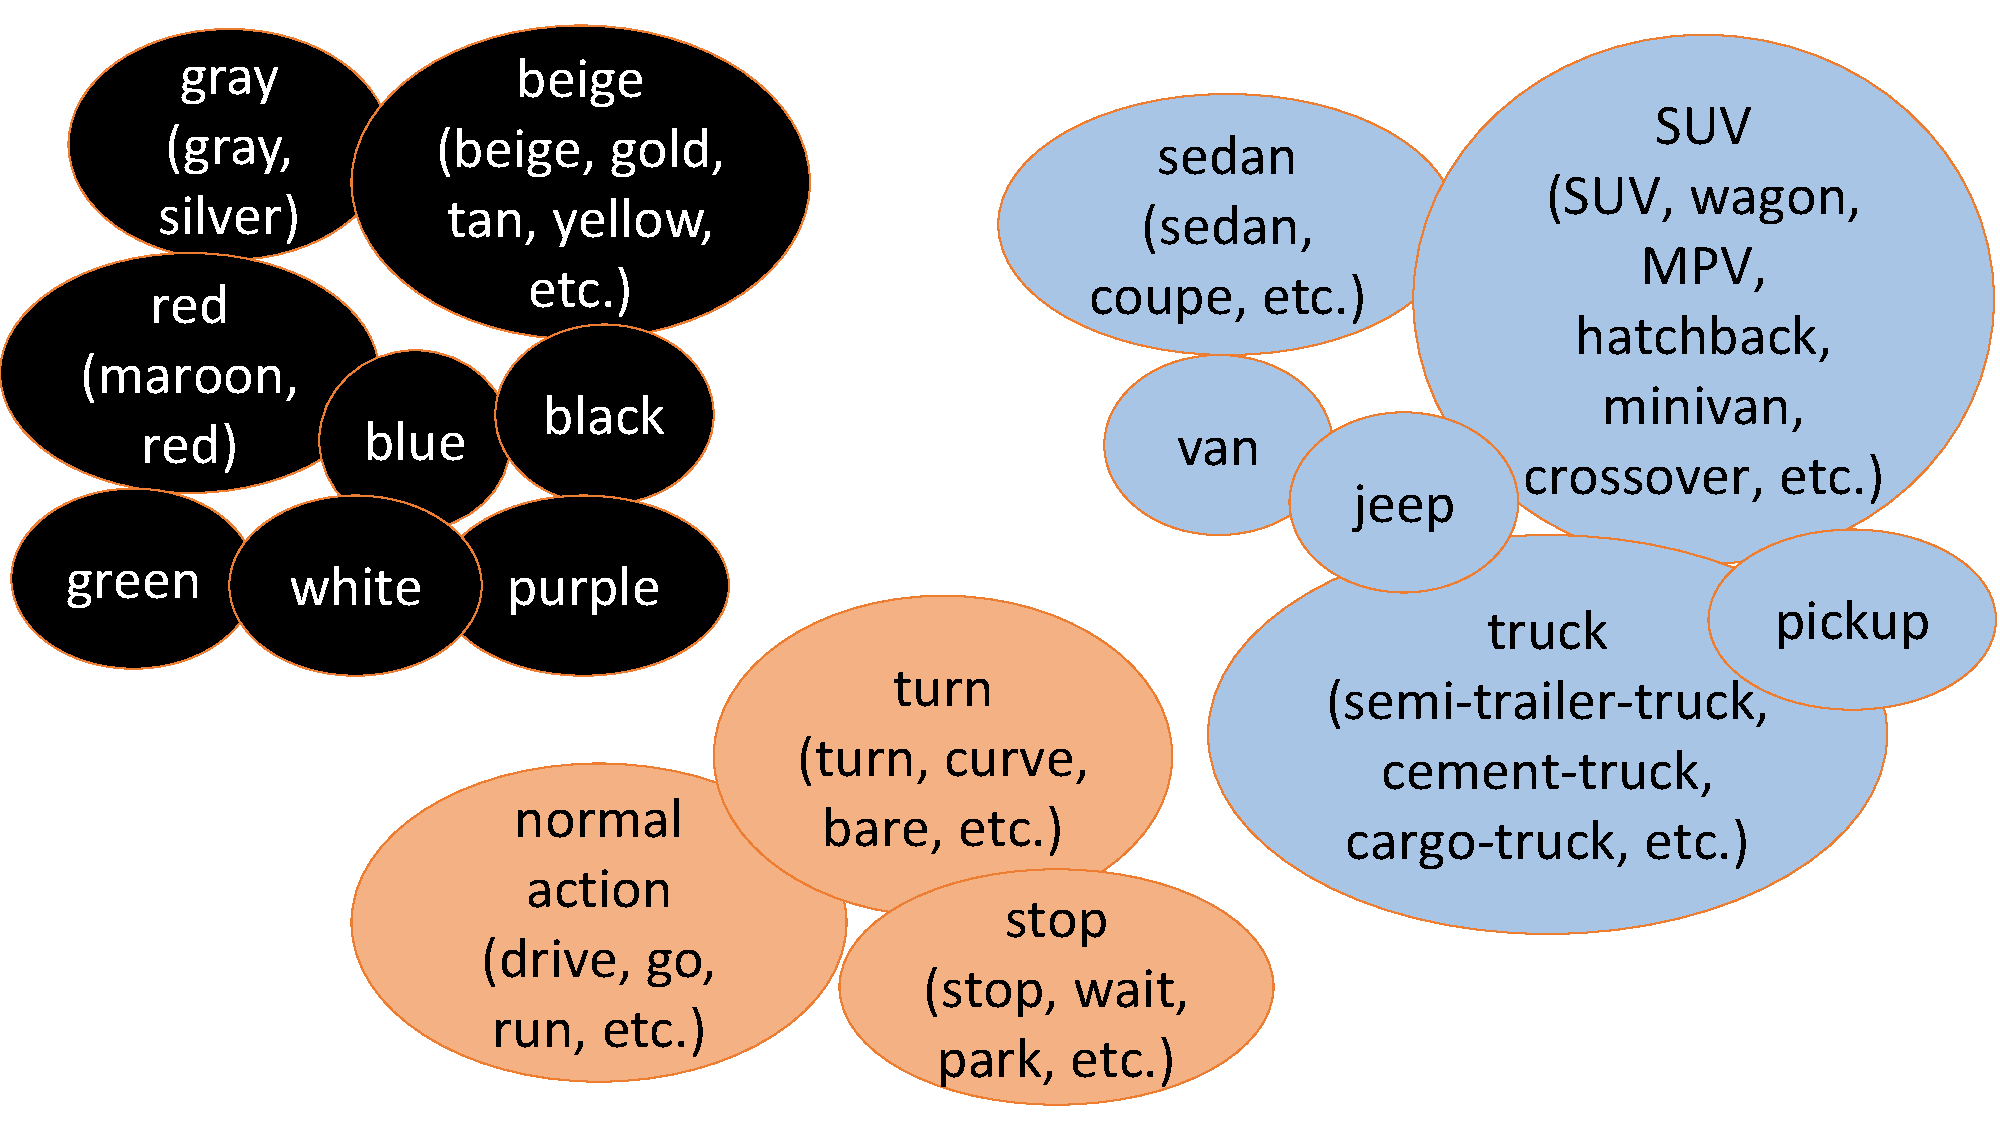
\includegraphics[width=\textwidth]{images/methods/group_example.pdf}
    \caption{How we categorize three attribute types. The black, orange, and blue shapes show the group of color, action, and vehicle type, respectively.}
    \label{fig:group_example}
\end{figure}

\begin{figure}[t!]
    \centering
    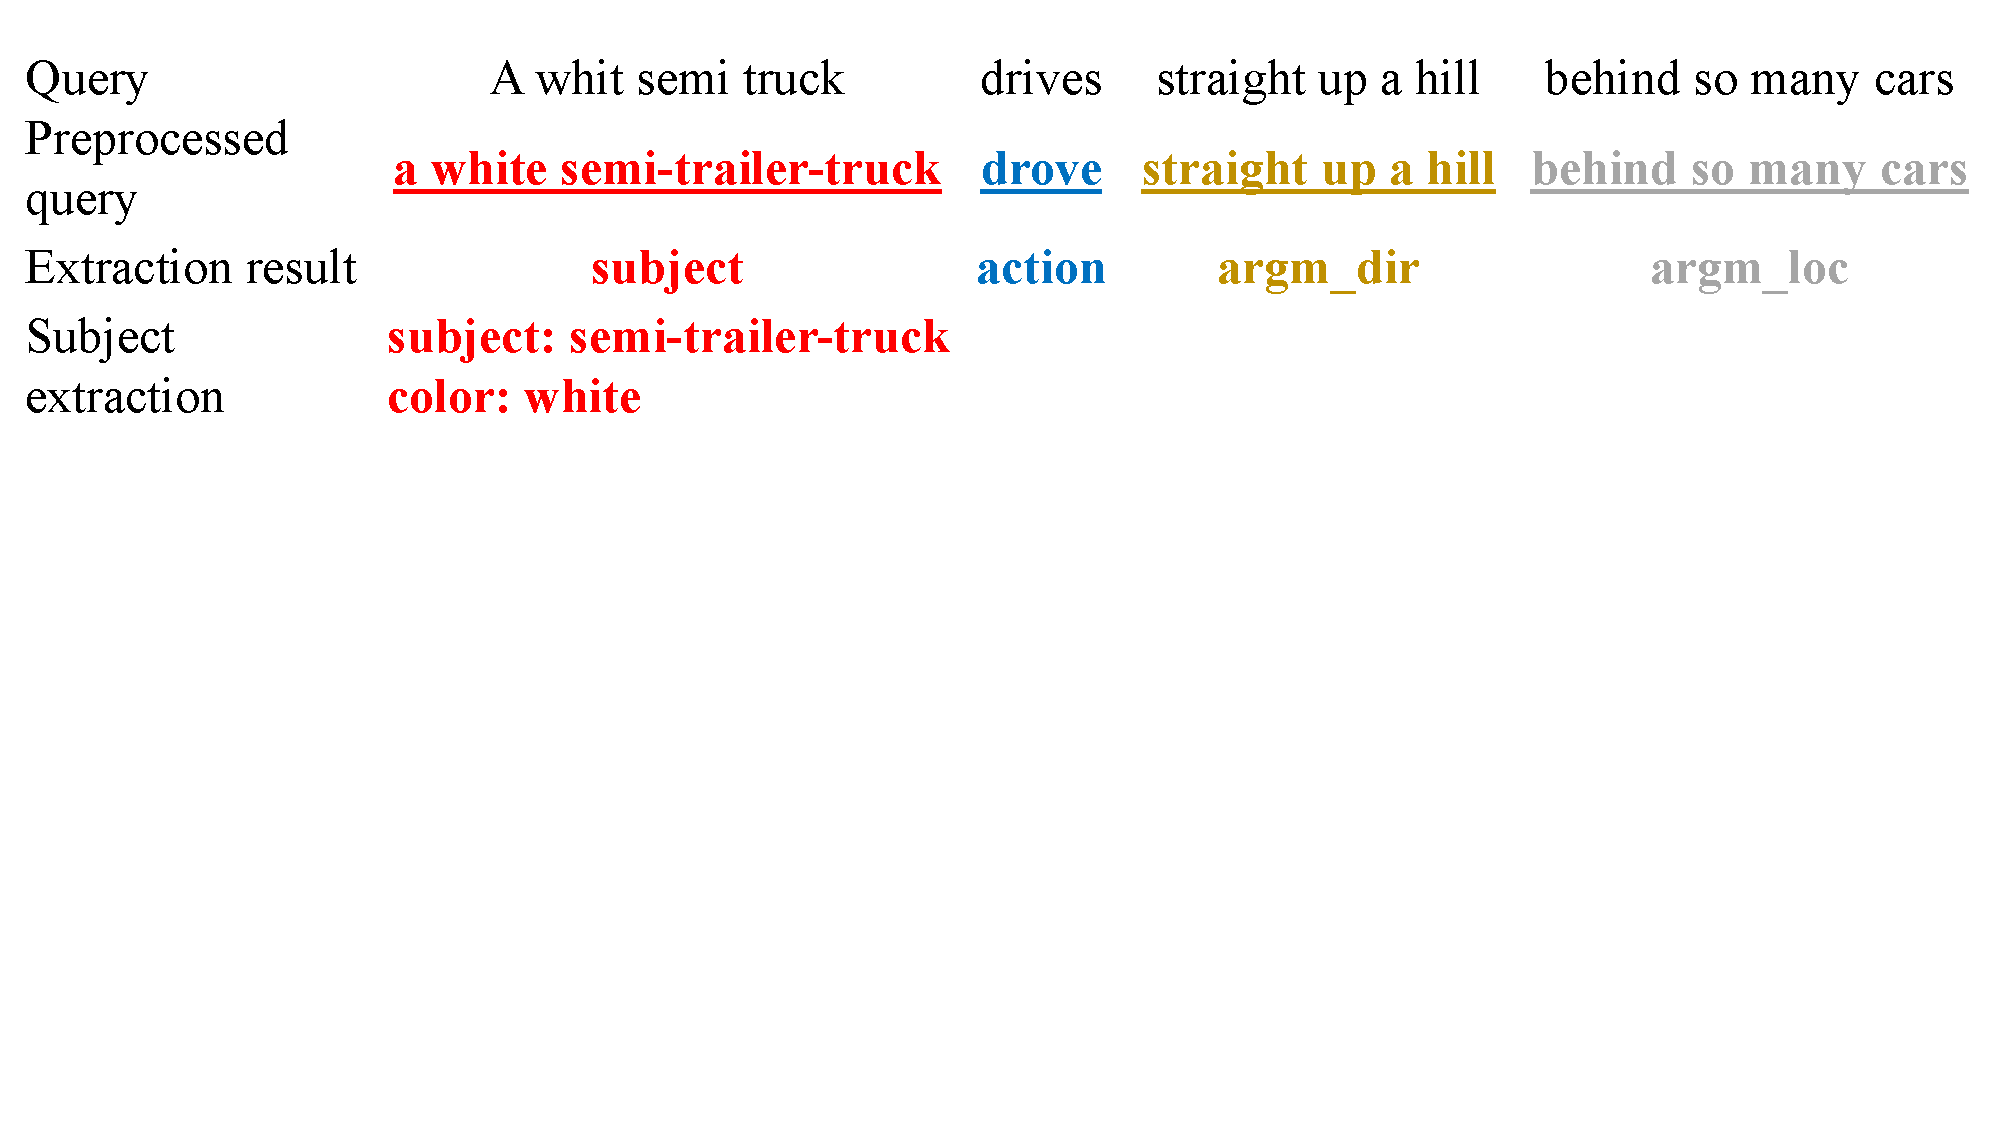
\includegraphics[width=\textwidth]{images/methods/text_extraction_example.pdf}
    \caption{An example of a query transformed and extracted through 2 stages of the heuristics method.}
    \label{fig:text_extraction_example}
\end{figure}
To make the SRL predictor work efficiently, the query needs to be corrected if it has wrong spelling. We use the Levenshtein distance metric to convert a target word to a source word in our defined vocabulary collection of vehicle attributes. To avoid the false convert, we set the condition of correcting a distance equal to 1 between the target word and the source word. We also add a rule to skip certain words which are not misspelled but have a distance of 1. For example, in the preprocessed query provided in Figure \ref{fig:text_extraction_example}, we have changed the wrong word \textit{“whit”} to \textit{“white”} but kept the word \textit{“so”} although it has the Levenshtein distance equal to 1 with the word \textit{“go”}. After this step, there is another collection containing rules to convert inconsistent words or phrases into a common one and/or verbs that are easily confused with nouns into past tense. As seen in the mentioned example, we have also made the word \textit{“semi truck”} (in the same group with \textit{“semi-truck”}, \textit{“tractor-trailer”}) become \textit{“semi-trailer-truck”}, and the word \textit{“drives”} become \textit{“drove”}. When finishing this stage, all of the essential terms related to traffic have been clear enough to be extracted.
\subsection{Extraction stage}
\begin{figure}[!htb]
    \centering
    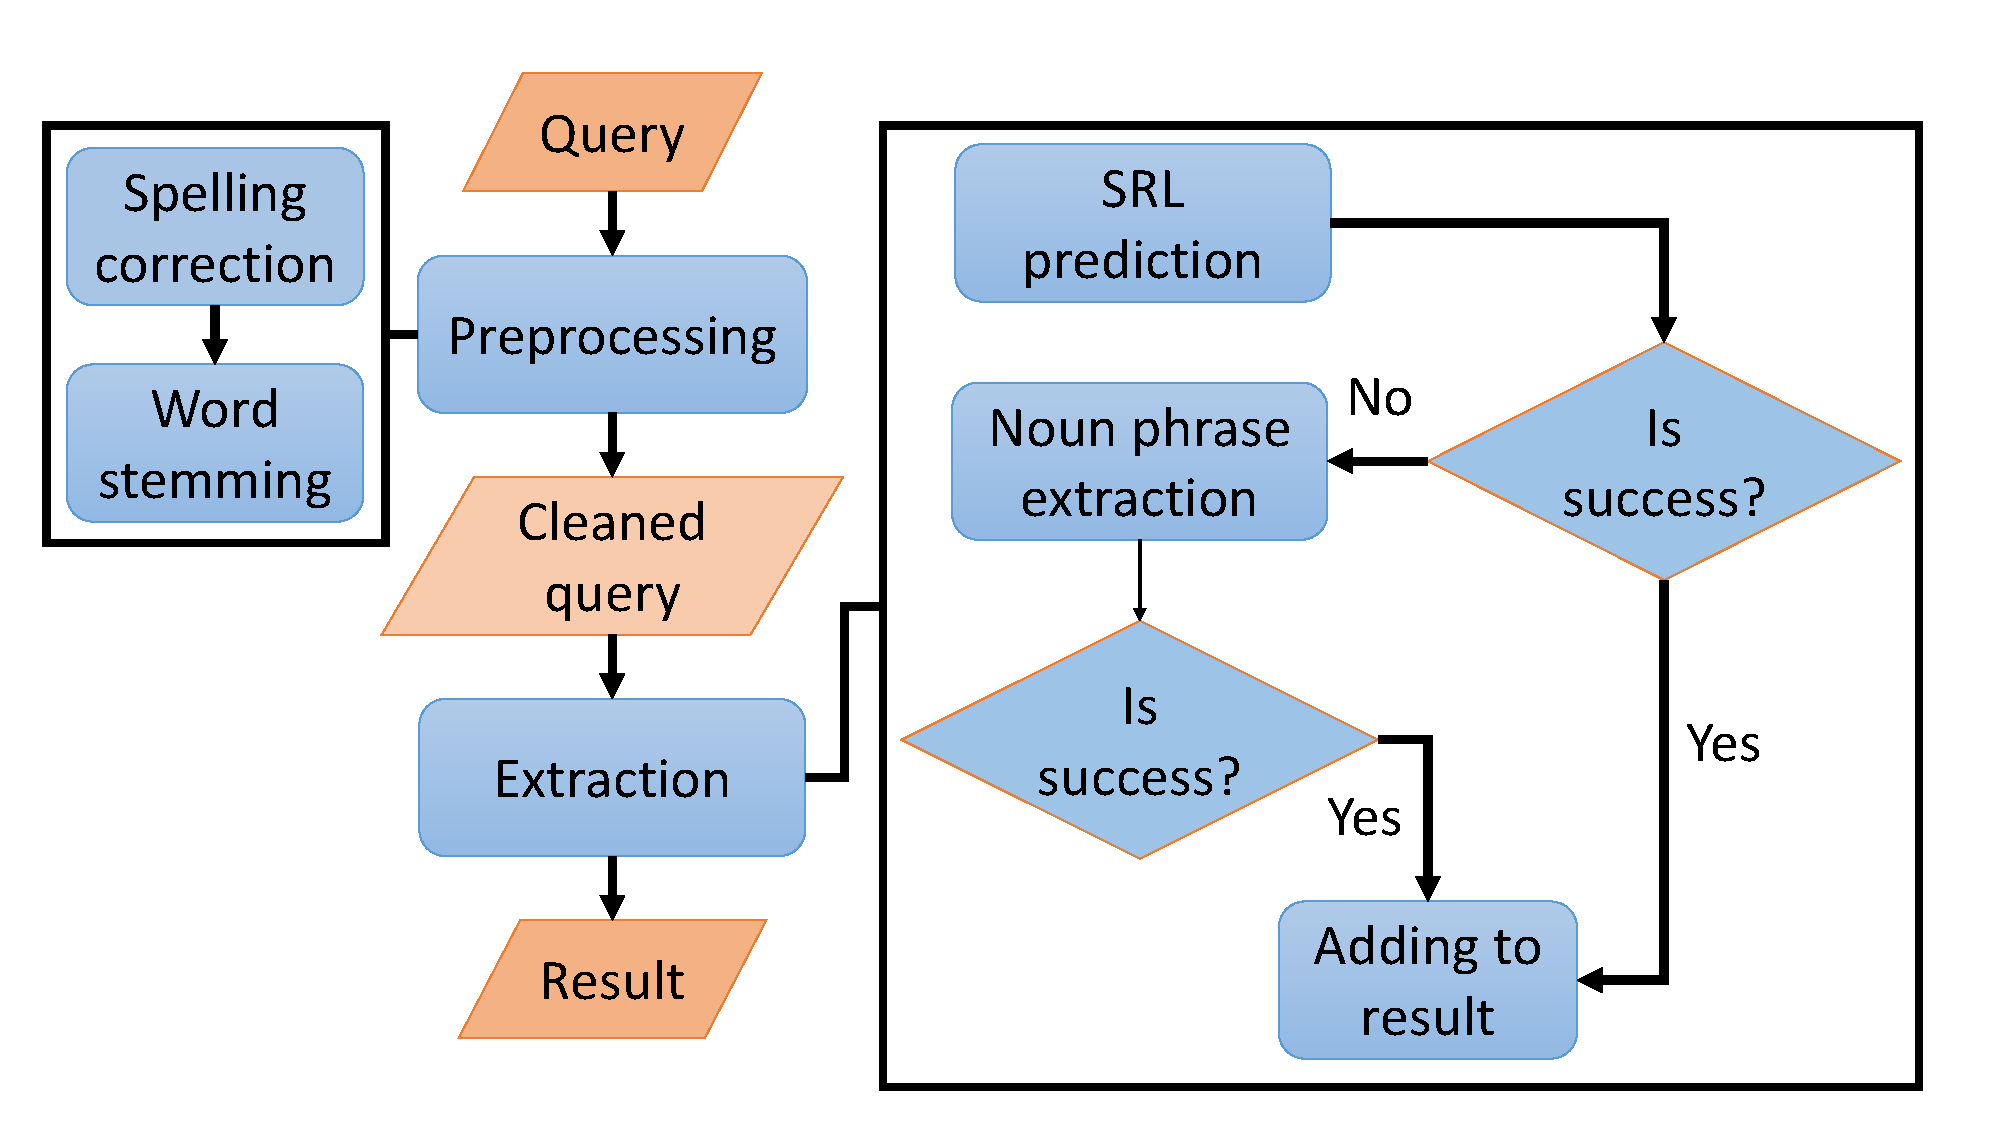
\includegraphics[width=\textwidth]{images/methods/stage_2_overview.pdf}
    \caption{An overview of the heuristic method to extract a query into SRL parts.}
    \label{fig:text_branch_stage_2_overview}
\end{figure}
For each query, a predictor toolkit is used to obtain parts of the SRL result. If the query is a complete sentence, the function will extract successfully. Otherwise, the query can be a noun phrase, and hence we must use another method to handle this. In this situation, we will collect the result if we can find the subject and confirm it as a vehicle type (i.e., \textit{a white truck}, \textit{a typical jeep}), or it will be skipped (i.e., \textit{straight on the main road}, \textit{light short to the right}).



% \section{Visual Attribute Extraction}
\label{sec:video_extraction}
\input{method_tex/vehcol_extraction}
\input{method_tex/action_detection}
\input{method_tex/relation_modeling}
\pagebreak
% \section{Retrieval model}
\label{sec:retrieval_model}
\subsection{Overview}
\begin{figure}[!htb]
    \centering
    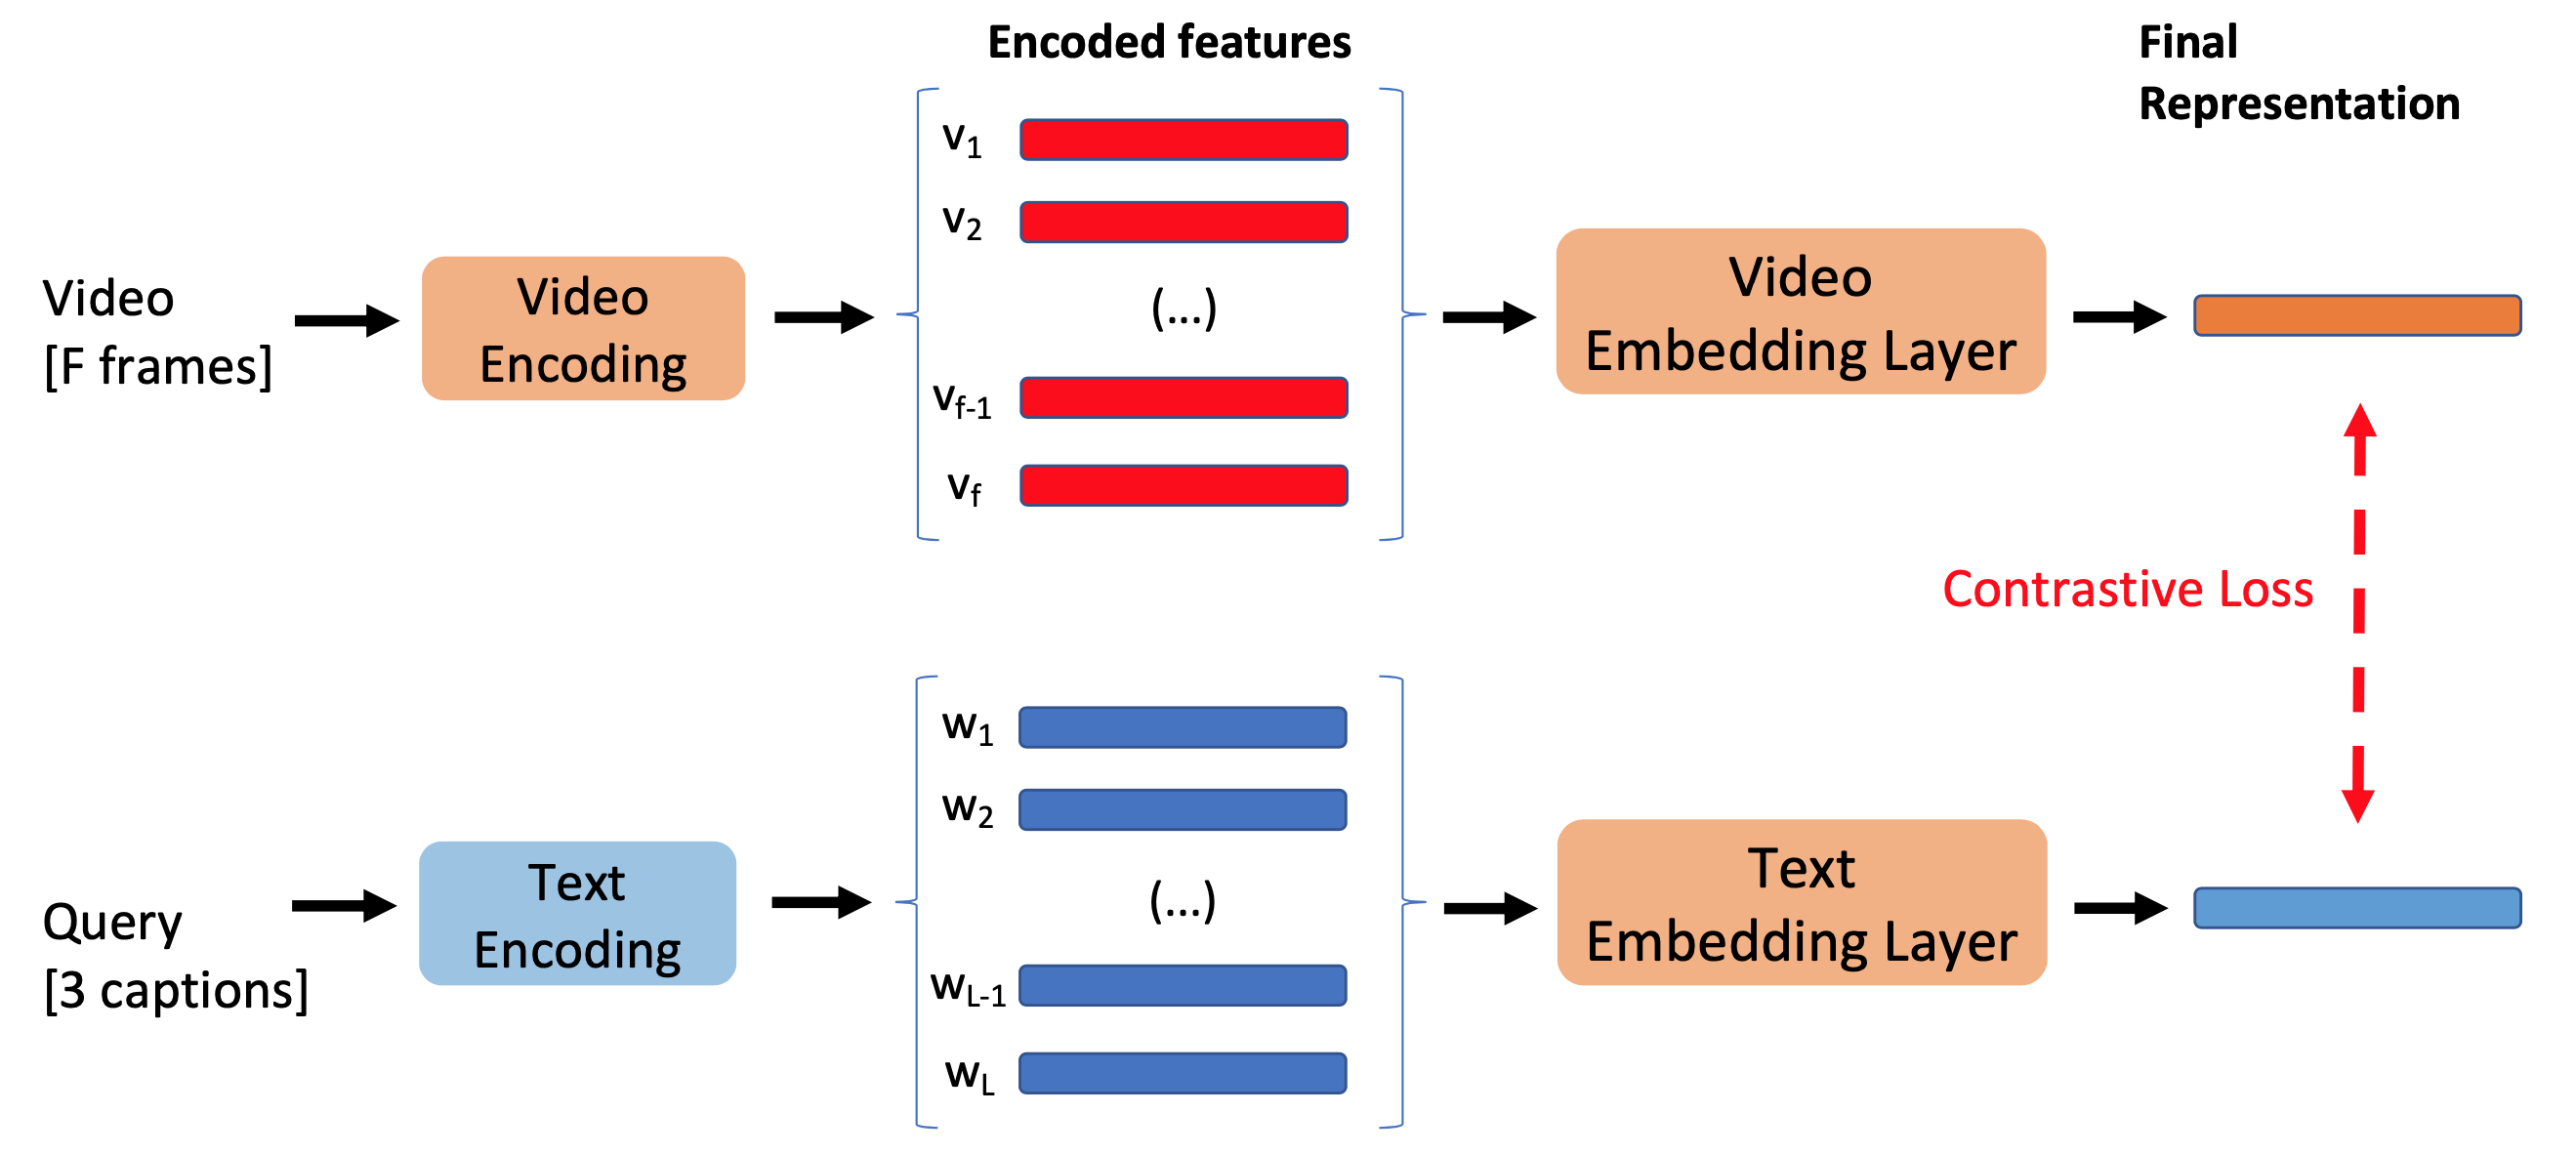
\includegraphics[width=\linewidth]{images/methods/retrieval_model.png}
    \caption{Retrieval model architecture.}
    \label{fig:ret_overview}
\end{figure}
Representation learning-based (RL-based) retrieval methods have shown potential results in various modalities. 
Especially for sequential data such as video and text, the attention mechanism provides a powerful technique for rich feature extraction, which leads to many success in cross-modalities learning tasks (as discussed in section \ref{sec:video-text_ret}). 
To efficiently apply this method to the vehicle-based retrieval problem, we employ a transformer-based architecture to learn the representation for video and text input, in which, the video encoded input is constructed from the target's essential appearance features. 
We inherit the embedding backbone of the COOT framework \cite{ging2020coot}, with some modification for better fit with our scenario.
Figure \ref{fig:ret_overview} summarizes our proposed approach.

\subsection{Representation learning}
\subsubsection{Query encoding [TODO: attribute-aware]}
In text branch, we can naively model the paragraph input in many different ways by choosing one from the combinations of three different sentences for each query.
However, we observe that the three descriptions can contain mutual meaning. For instance, the later caption may have reference to the former one.
\begin{itemize}
    \item \textit{\underline{Yellow car} keeps straight.}
    \item \textit{\underline{A yellow coupe} keeps straight before a diverging road.}
    \item \textit{There was a black pickup behind \underline{the vehicle}.}
\end{itemize}
Thus, in the encoding step, we aim to concatenate those descriptions as a whole paragraph, which provides the complete information for a specific target track.
For a query $q_i = [s_{i=1:3}]$, the preparing process is setup as follow:
\begin{enumerate}
    \item Splitting each sentence $s_i$ into a list of tokens.
    \item Encoding each token to a $d_{word}$-dimension vector. Consequently, the sentence vector is therefore a list of word vectors.
    \item Concatenating the three-sentence vectors as a final representation $\mathbf{v_{query}}$ for the query.
\end{enumerate}

\subsubsection{Video encoding}
In video branch, the video track also contains the local information of the target vehicle, which is usually the main subject and provides potential visual attributes described in the given query. For that reason, different from the original COOT method, we also include the target's attribute features in the video encoding vector. \\
In the COOT framework, given a video $V$ with $F$ frames, the video encoding is constructed by concatenating all $F$ frame-level feature $d_F$-dimension vectors, which are extracted by pretrained backbones.
For each frame, the feature vectors, enriched by deep neural networks pretrained on large benchmark datasets, contain helpful global information but lack local ones, which could be the target vehicles we need to focus on in the CityFlow-NL setup. 
From this point of view, we modify the frame-level encoded vectors with the following strategy.
Let $\mathbf{v_{frame}}$ denotes the feature vector for each frames in a video track, $\mathbf{v_{frame}} \in \mathbb{R}^{d_f}$. We define this feature as a combination of three sources:
\begin{enumerate}
    \item \textbf{Global context information ($\mathbf{v_{global}}$)}. The element aim to provide general information of each video frame.
    \item \textbf{Attributes representation ($\mathbf{v_{veh}}$)}. The compact feature produced by the attribute classifiers (section \ref{sec:vehcol_extraction}) provides the important details of the target vehicle that the model needs to focus on during the retrieval process.
    \item \textbf{Target vehicle location ($\mathbf{v_{loc}}$)}. The relative location and size of target vehicle at each time step, provide the main subject's movement trajectory information.
\end{enumerate}
For the $\mathbf{v_{global}}$, we apply the same approach as the COOT framework, which is the global feature extracted by the ResNet-152 \cite{he2016deep} pretrained on ImageNet \cite{russakovsky2015imagenet}. 
The $\mathbf{v_{veh}}$ is constructed as a concatenation of color and vehicle-type encoded vectors ($\mathbf{v_{veh-col}}$, $\mathbf{v_{veh-type}}$) provided by the corresponding encoders $E_{col}$ and $E_{veh}$, details in \ref{sec:vehcol_extraction}.
\[ 
\mathbf{v_{veh}} = concat(\mathbf{v_{veh-col}}, \mathbf{v_{veh-type}})
\]
And the vehicle location component is constructed from the bounding box coordinates at a given frame.
\[
\mathbf{v_{loc}} = [x/W, y/H, w/W, h/H]
\]
where $(x, y, w, h)$ denotes the box top-left coordinate, width, height. $(W, H)$ are respectively the width, height of the video frame. 
\begin{figure}[!h]
    \centering
    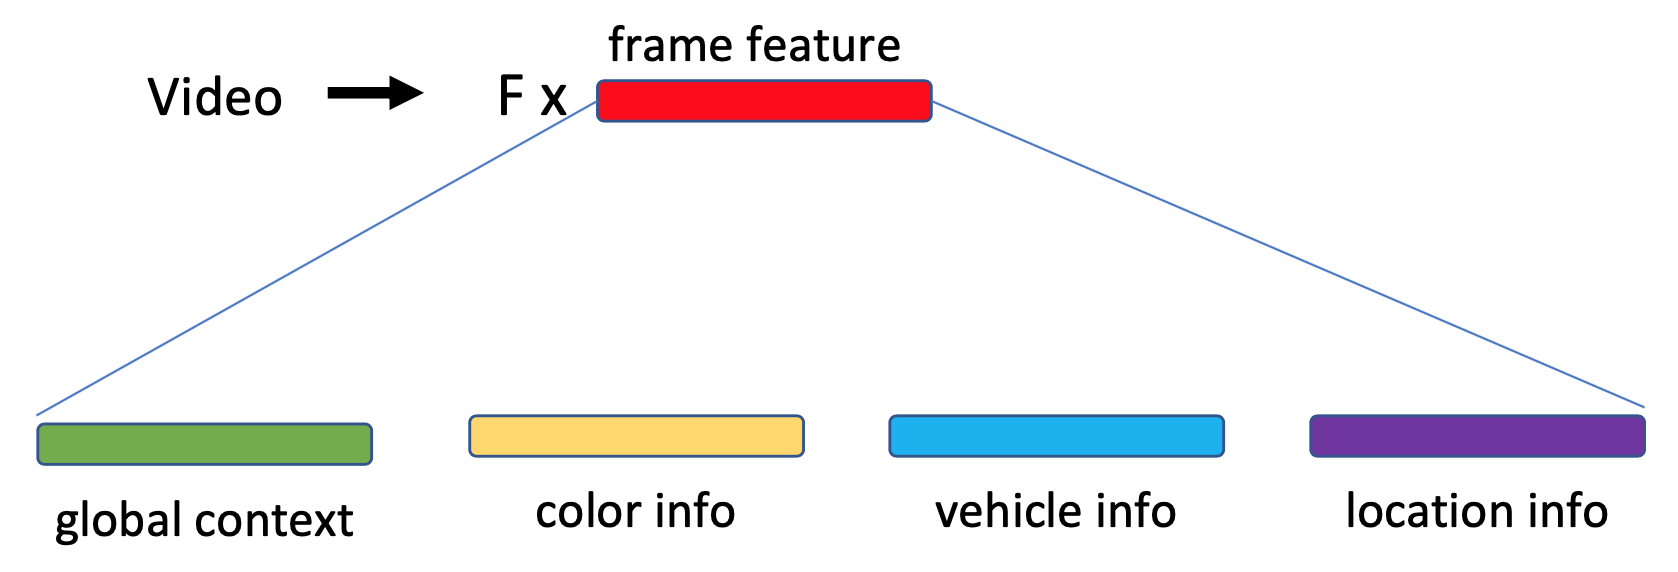
\includegraphics[width=\linewidth]{images/methods/video_encoding.png}
    \caption{Video encoding procedure.}
    \label{fig:video_encoding}
\end{figure}

In total, the frame encoded feature is modelled as:
\[
\mathbf{v_{frame}} = concat(\mathbf{v_{global}}, \mathbf{v_{veh}}, \mathbf{v_{loc}})
\]
which contains both global context and target's descriptive informations. And the final encoding for each F-length video track $\mathbf{v_{track}}$ is the combination of F frame-level features, resulting in $F \times d_f$-dimension vector (illustrated in Figure \ref{fig:video_encoding}).
The track/query representation feature ($\mathbf{v_{track}}$, $\mathbf{v_{query}}$) is then fed forward through the corresponding encoding blocks to obtain the final embedding vectors.

\subsection{Loss function}
To efficiently train the retrieval model, we inherent the alignment loss of Zhang et al. \cite{zhang2018cross}, which leverage the contrastive loss to enforce the positive samples to stay closer and the negative ones far apart. 
Given a positive sample $P = (q_i, v_i)$, set of two negative pairs $N = \{({q_i}', v_i), (q_i, {v_i}')\}$ and a margin $\alpha$, they define the following loss:
\begin{equation}
\begin{split}
    L(P, N, \alpha) = & \mathrm{max}(0, \alpha + D(q_i, v_i) - D({q_i}', v_i)) + \\ 
    & \mathrm{max}(0, \alpha + D(q_i, v_i) - D(q_i, {v_i}'))
\end{split}
\end{equation}
% \begin{align}
%     L(P, N, \alpha) = & \mathrm{max}(0, \alpha + D(q_i, v_i) - D({q_i}', v_i)) + \\ 
%     & \mathrm{max}(0, \alpha + D(q_i, v_i) - D(q_i, {v_i}'))
% \end{align}
Where $D(x, y) = 1 - \frac{x^{\top}y}{\left \| x \right \|\left \| y \right \|}$ denotes the cosine distance between two representation vectors, $q_i$ and $v_i$ indicate the embedding vectors of query and video respectively. \\
The alignment loss is defined as follow.
\begin{align}
    L_{align} = \sum_{k \in B, i, {k}'\neq k, {i}'\neq i} L((q_i, v_i), \{({q_i}', v_i),(q_i, {v_i}')\}, \beta)
\end{align}
where $B$ denotes the batch of samples at each training step, $\beta$ is the constant margin.
% \section{Relation modeling}
\label{sec:relation}
% \section{Refinement method}
\label{sec:refinement}
In the retrieval module (section \ref{sec:retrieval_model}), we have encoded the visual feature using information from color, vehicle types, and location of the target object. However, we did not exploit the motion features of the tracked objects. Therefore, we build another module to further refine the previously obtained results. In particular, this module focuses on the assessment of similar motion extracted from the query and the video track. The annotation action results of the text are retrieved from the second phase of SRL extraction (section \ref{sec:text_extraction}). Meanwhile, the annotation results of the video action are obtained from the stop and turn detector (section \ref{sec:action_detection}). The retrieval results are refined with the following priorities, i.e., motion, color, and vehicle types. The details of the refinement process are as follows:


% \chapter{Experiment}
\label{chap-experiment} 
\begin{ChapAbstract}
In this chapter, we describe the experiment dataset, evaluation metrics, and challenge platform. Besides, we provide the details configurations and implementation details of our proposed method. Based on that, we also analyze the result with on our observations.
\end{ChapAbstract}
% Dataset and evaluation measures (The authors can either use the default description in the
% template of write this part by themselves. The dataset-related papers should be cited.)
% Implementation details
% Detailed description of training protocols


\section{Dataset and evaluation measures}

\subsection{FLARE22 dataset}

The FLARE2022 dataset is curated from more than 20 medical groups under the license permission, including MSD \cite{simpson2019MSD}, KiTS \cite{KiTS,KiTSDataset}, AbdomenCT-1K \cite{AbdomenCT-1K}, and TCIA \cite{clark2013TCIA}. 
It is extended from the FLARE 2021 Challenge from fully supervised settings to a semi-supervised setting that focuses on how to use unlabeled data. Specifically, they provide a small number of labeled cases (50) and a large number of unlabeled cases (2000) in the training set, 50 visible cases for validation, and 200 hidden cases for testing. The segmentation targets include 13 organs: liver, spleen, pancreas, right kidney, left kidney, stomach, gallbladder, esophagus, aorta, inferior vena cava, right adrenal gland, left adrenal gland, and duodenum. Compare to the FLARE 2021 challenge, the dataset is 4x larger and the segmentations targets are increased to 13 organs.

\subsection{Evaluation metrics}

The evaluation measures consist of two accuracy measures: the region-based Dice Similarity Coefficient (DSC) and the boundary-based Normalized Surface Dice (NSD) \cite{nikolov2018deep}, and three running efficiency measures: running time, area under GPU memory-time curve, and area under CPU utilization-time curve. All measures will be used to compute the ranking. Moreover, the GPU memory consumption has a 2 GB tolerance.

Let $G$, $S$ denote the ground truth and the segmentation result, respectively. $|\partial G|$ and $|\partial S|$ are the number of voxels of the ground truth and the segmentation results, respectively. Both metrics take the scores in $[0, 1]$ and higher
scores indicate better segmentation performance. We formulate the definitions of the two measures in the two following sections.

\subsubsection{Dice Similarity Coefficient}

The Dice similarity coefficient, also known as the Sørensen–Dice index or simply Dice coefficient, is a statistical function which measures the similarity between two sets of data. The DSC has become arguably the most widely used tool in several segmentation benchmarks \cite{heller2021state}, \cite{bilic2019liver}.  In term of segmentation task, it is used to evaluate the region overlap between the predicted and the target mask. The formulation is as follows:

\begin{align}
        \text{DSC(G,S)} &= \frac{2|G \cap S|}{|G| + |S|}
\end{align}

\subsubsection{Normalized surface Dice}

Despite its popularity, DSC does not take boundary precision into account, while that is a crucial aspect in clinical medical tasks. In contrast, NSD is sensitive to this boundary error and is used to evaluate how close the segmentation and ground truth surfaces are to each other at a specified tolerance $\tau$. NSD can be formualzed as below:

\begin{align}
        \text{NSD(G,S)} &= \frac{|\partial G \cap \mathcal{B}^{\tau}_{\partial S}| +  |\partial S \cap \mathcal{B}^{\tau}_{\partial G}|}{|\partial G| + |\partial S|}
\end{align}

where $\mathcal{B}^{\tau}_{\partial G} = \{ x \in \mathcal{R}^3 | \exists \tilde{x} \in \partial G, ||x - \tilde{x} || \leq \tau$, $\mathcal{B}^{\tau}_{\partial S} = \{ x \in \mathcal{R}^3 | \exists \tilde{x} \in \partial S, ||x - \tilde{x} || \leq \tau$ denote the border region of the ground truth and the segmentation surface at tolerance $\tau$, respectively. According to \cite{AbdomenCT-1K}, FLARE22 Challenge uses $\tau = 1\text{mm}$.

\subsection{Implementation details}
\subsubsection{Environment settings}
The development environments and requirements are presented in Table~\ref{table:env}.


\begin{table}[!h]
\caption{Development environments and requirements.}\label{table:env}
\centering
\begin{tabular}{ll}
\hline
Windows/Ubuntu version       & Ubuntu 18.04.5 LTS\\
\hline
CPU   & Intel(R) Xeon(R) Silver 4210R CPU @ 2.40GHz \\
\hline
RAM                         &1$\times $32GB; \\
\hline
GPU (number and type)                         & One Quadro RTX 5000 16G\\
\hline
CUDA version                  & 11.6\\                          \hline
Programming language                 & Python 3.10\\ 
\hline
Deep learning framework & Pytorch (Torch 1.11.0, torchvision 0.12.0) \\

\hline
\end{tabular}
\end{table}

\vspace{-0.5cm}

\subsubsection{Preprocessing protocols}

In the beginning of both training and inference phase, the CT volumes are splitted into slices of 2D images before applying Windowing CT. As mentioned before, we keep the original size of the volumes. Then,for each of these slices, Windowing CT is applied with three different settings to generate three version of each. The three settings aim to highlight three particular parts of the human organs, which are: the chest, the abdomen, and the spine. Detailed configuration is shown in Table \ref{table:window_params}

\subsubsection{Training protocols}

Currently, we find that using only simple 2D transform functions such as horizontal/vertical flipping or rotating might be enough for both modules to generalize. In the training stage, the Reference module follow traditional training process, in which two models are concurrently trained. For the Propagation module, we inherit the same process as in \cite{stcn21cheng} which samples 3 neighboring slices at a time.

Table \ref{table:training1} and Table \ref{table:training2} mention the training protocols for Reference module and Propagation module, respectively. In both settings, we use the original-sized images, which is $[512, 512]$ for the training and inference phases. 

\begin{table*}[!h]
\caption{Training protocols for Reference module: CPS of TransUnet and Efficientnet DeeplabV3+ }
\label{table:training1}
\begin{center}
% \resizebox{0.47\textwidth}{!}{
\begin{tabular}{ll} 
\hline
Network initialization         & Random initialization\\
\hline
Batch size                    & 2 (labeled) $+$ 2 (unlabeled) \\
\hline 
Patch size & None  \\ 
\hline
Total iterations & 50000 \\
\hline
Optimizer          & AdamW          \\ \hline
Initial learning rate (lr)  & 0.0001 \\ \hline
Lr decay schedule & multiplied by 0.5 every iteration at $[40000, 45000]$ \\
\hline
Training time                                           & 48 hours \\  \hline 
Number of model parameters & \begin{tabular}[c]{@{}l@{}}105M (TransUnet Resnet50) +\\ 11M  (Efficientnet DeeplabV3+) \footnote{Pytorch}\end{tabular} \\
\hline
Number of flops &  \begin{tabular}[c]{@{}l@{}}108G (TransUnet Resnet50) +\\1,3G (Efficientnet DeeplabV3+)  \footnote{Pytorch}\end{tabular} \\
% {108G (TransUnet Resnet50) + 1,3G (Efficientnet DeeplabV3+)  \footnote{Pytorch}} \\ 
% & \\
\hline
\end{tabular}
% }
\end{center}
\end{table*}


\begin{table*}[h]
\caption{Training protocols for Propagation module: STCN with Resnet backbone }
\label{table:training2}
\begin{center}
% \resizebox{0.47\textwidth}{!}{
\begin{tabular}{ll} 
\hline
Network initialization         & Random initialization\\
\hline
Batch size                    & 8 \\
\hline 
Patch size & None  \\ 
\hline
Total iterations & 50000 \\
\hline
Optimizer          & AdamW          \\ \hline
Initial learning rate (lr)  & 0.0001 \\ \hline
Lr decay schedule & multiplied by 0.5 every iteration at $[40000, 45000]$ \\
\hline
Training time                                           & 48 hours \\  \hline 
Number of model parameters    & 54,416,065 \footnote{Pytorch} \\ \hline
\end{tabular}


\end{center}
\end{table*}

\vspace{-0.5cm}
\subsubsection{Testing protocols}

In the inference phase, after applying windowing CT technique for pre-processing, we then resize all the slices to $512 \times 512$ prior to predicting. When the model generate a mask prediction, which apparently the same size as 512, we interpolate that to the original size.

Initially, in the Reference stage, we do not forward the entire volume since it would increase the GPU resource tremendously. Here, we follow a simple strategy which is uniform sampling. For each CT volume, we sample a slice every 5 steps, then group them as a batch and forward through the Reference module. As mentioned earlier, the Reference module consists of two 2D segmentation models: TransUnet with Resnet50 as backbone and DeeplabV3+ with EfficientNetB3 as backbone, they are used simultaneously to generate the prediction.
The masks outputed from this module are filtered once more to select only potentially informative slices and its annotation. Another sampling strategy is used here, to pick the possible slices, we iterate through them and calculate the areas of the visible organs. Then for each organ, we choose the slice that have the largest area of it, which leaves us with only 13 candidate slices maximum.

Then comes the Propagation module, with these only 13 slices, this module has to propagate all the information across the remaining slices. This also includes a propagation strategy as well. For each of the annotated slices as the pivot points,
the module perform bidirectional propagation strategy, then sum them up before finally deciding which classes they are. 
In more detail, the STCN architecture inside the Propagation module has a memory bank that can store up past information and use them to predict the current input. For every $k_1$ frame, the bank encode the frame and save the information once, then find top $k_2$ encoded frames that is most similar with the current one to generate the mask. In addition, the memory bank gets flushed every $k_3$ frames stored. In all our experiment, we find that $k_1 = 5$, $k_2 = 20$ and $k_3 = 200$ gives best overall results while keeping the GPU memory not overloaded.

Regarding the pseudo-labeling process, we use multiple trained CPS to create a pool of pseudo-labeled data and measure the uncertainty between them. Following the Equation \ref{eqn:uncertainty}, we filter out samples with scores higher than $0.9$ and use them for the next training cycle. The cycle loops until all unlabeled samples become high quality.

% The validation performance (DSC) comparisons between with and without using unlabelled
% images
% Visualized examples of successful and failed cases
% Segmentation efficiency analysis
% Limitations and future work

\section{Quantitative results}
\label{sec:quantitative}

Here we present both quantitative and qualitative results of our proposed method. We also include the ablation study (Table \ref{table:ablation_study}) to further analyze the effectiveness of each of our modules. 

\begin{table}[h]
\centering
\caption{Comparison between using and not using the pseudo labels as supervised training data. The model that is used for the report is TransUnet \cite{transunet21chen}. The highlighted figures emphasize the highest values in each row. The Dice Scores are reported on the public test set, and are given from the public leaderboard.}
\footnotesize
\begin{tabular}{| c | c | c | c | }
\hline
\textbf{Number of pseudo-labeled samples} & 0 & 200 & 700  \\
\hline
\textbf{Liver} & 0.9141  & 0.9555 & \textbf{0.9604} \\
\textbf{RK} & 0.645 & 0.7944 & \textbf{0.8014} \\
\textbf{Spleen} & 0.8071 & 0.9144 & \textbf{0.9255}	\\
\textbf{Pancreas} & 0.6152 & 0.7309 & \textbf{0.7567}	\\
\textbf{Aorta} & 0.8992 & 0.9272 & \textbf{0.9335} \\
\textbf{IVC} & 0.7398 & 0.7967 & \textbf{0.8207} 	\\
\textbf{RAG} & 0.5786 & 0.6507 & \textbf{0.6545} 	\\
\textbf{LAG} & 0.4376 & \textbf{0.6179} & 0.6138 	\\
\textbf{Gallbladder} & 0.474 & \textbf{0.5889} & 0.5885	\\
\textbf{Esophagus} & 0.74 & \textbf{0.7784} & 0.7783 	\\
\textbf{Stomach} & 0.7678 & 0.8403 & \textbf{0.8424} 	\\
\textbf{Duodenum} & 0.4425 & 0.5617 & \textbf{0.5679}	\\
\textbf{LK} & 0.7015 & \textbf{0.8112} & 0.8026 \\ 
\textbf{Mean DSC} & 0.674 & 0.7668 & \textbf{0.7728} \\ 

\hline
\end{tabular}
\label{table:unlabeled}
\vspace{-2mm}
\end{table}

Some interesting insights can be spotted in Table \ref{table:unlabeled}. Overall, we can see that using the pseudo-labeled data for training, helps boost the performance of the model by a great amount. Unfortunately, we have yet to fully explore every unlabeled sample (only 700 samples were used for training in our submission), but intuitively, the number of used unlabeled samples is likely to be directly proportional to the evaluation result. Another notable observation is that the DSC for some small human organs (gallbladder and adrenal glands) can hardly be improved because of the class imbalance problem. %(as referred in \ref{sec:limitation}) 

\begin{table}[h]
\centering
\caption{Ablation experiment on each proposed modules and techniques. Scores are reported on the public test set, which in available on the public leaderboard.}
\footnotesize
\begin{tabular}{| c | l | c | c | c | c |}
\hline
\textbf{No.} & \textbf{CPS} & \textbf{Windowing CT} & \textbf{UE} & \textbf{MP} & \textbf{Mean DSC} \\ 
\hline
1  &            &  & & & 0.547   \\
2  & $\checkmark$ &            &            & & 0.762   \\
3  & $\checkmark$ & $\checkmark$ & $\checkmark$ & & 0.770   \\
4  & $\checkmark$ & $\checkmark$ & $\checkmark$ & $\checkmark$ & 0.784   \\
\hline
\end{tabular}
\label{table:ablation_study}
\vspace{-2mm}
\end{table}

Table \ref{table:ablation_study} shows that each module contributes to the final score of our submission. The third and fourth rows where both Cross Pseudo Supervision (CPS) and Uncertainty Estimation (UE) is used mean that pseudo-labels that are qualified by UE are used as supervised inputs in CPS workflow whereas the remaining unlabeled data are used as unsupervised inputs. Noticeably, in the fourth row, with the Mask propagation (MP) applied, DSC score is enhanced. It is surprising that MP only looks upon the minority of the slices to fully propagate through the whole volume. We recommend looking at the qualitative result in Section \ref{sec:qualitative} to fully understand what each component contributes to the total score. The detailed evaluation for our final submission on the public test set is shown in Table  \ref{table:submission}. 

\begin{table}[h]
\centering
\caption{The final evaluation score for our final submission on the public test set}
\footnotesize
\begin{tabular}{| c | l | c | c | c | c | c |}
\hline
\textbf{Mean DSC} & \textbf{Liver} & \textbf{RK} & \textbf{Spleen} &	\textbf{Pancreas} &	\textbf{Aorta} &	\textbf{IVC} \\
\hline
0.7841 &	0.9591 &	0.8149 &	0.9244 &	0.7499 &	0.9383 &	0.8262 \\
\hline
\hline
\textbf{RAG} &	\textbf{LAG} &	\textbf{Gallbladder} &	\textbf{Esophagus} &	\textbf{Stomach} &	\textbf{Duodenum} &	\textbf{LK} \\
\hline
0.6456 &	0.601 &	0.6877 &	0.7986 &	0.8446 &	0.5808 &	0.8219   \\

\hline
\end{tabular}
\label{table:submission}
\vspace{-2mm}
\end{table}



\section{Qualitative results}
\label{sec:qualitative}

\subsection{Overall}

Looking at examples that are well-predicted by our approach in Fig \ref{fig:qualitative} (1b, 2b, 3b), it demonstrates good segmentation masks with clear and smooth mask boundaries. Some small organs can also be seen segmented successfully and precisely meaning that both proposed modules can work effectively with organs having various sizes. For reference, we use \cite{py06itksnap} for all the CT volume visualization in our project.

\begin{figure}[!h]
\centering
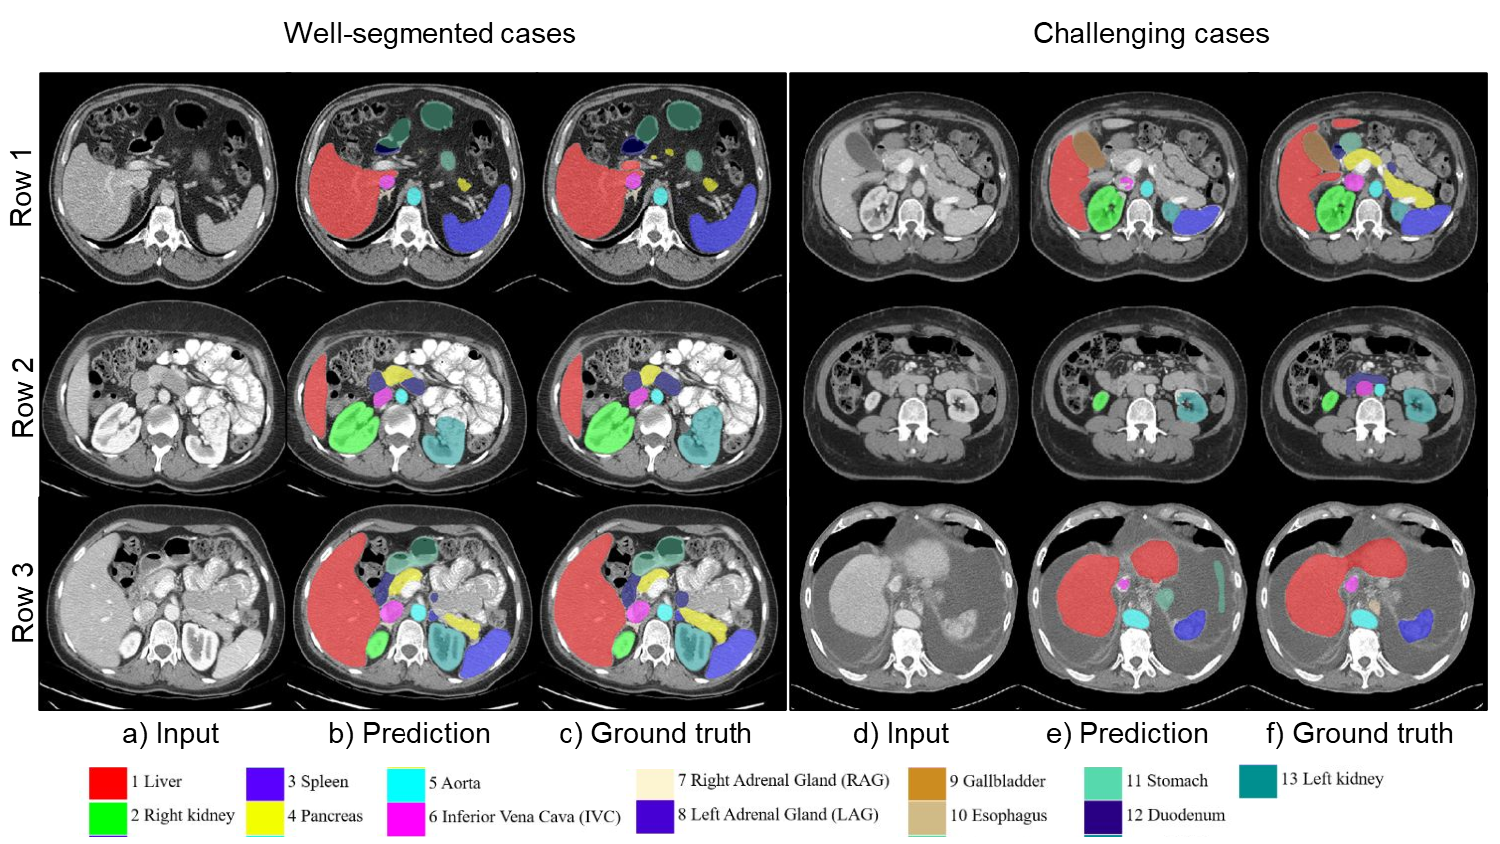
\includegraphics[width=\textwidth]{content/resources/new_images/qualitative.pdf}
\caption{Qualitative results from the validation set. We illustrate both well-segmented and challenging examples for our proposed segmentation pipeline}
\label{fig:qualitative}
\end{figure}

On the other hand, our models suffer from various difficult cases where organs are missing. Generally, there are two cases that negatively affect our approach:

\begin{enumerate}
    \item Relatively small organs (adrenal glands (Fig \ref{fig:qualitative} (1e)), gallbladder (Fig \ref{fig:qualitative} (1e)), and esophagus (Fig \ref{fig:qualitative} (3e))) account for the lowest DSC since they usually are failed to be identified by the Reference module.
    \item Other organs (pancreas (Fig \ref{fig:qualitative} (1e)) and duodenum (Fig \ref{fig:qualitative} (2e))) despite having a larger size, yet their lengths on the axial plane are short and sometimes occluded by many surrounding organs, which can affect how the information propagating through the slices, causing class confusion in the result. 
\end{enumerate}

Furthermore, due to our two-staged pipeline, for the results of the second stage to be good really relies on the first stage's performance.  If the reference stage miss-segments any organ, that one will be missed during the entire propagation process. Having said that, this issue mostly just occurs in organs that have a short-size length on the axial plane.  


\subsection{Improvement of Mask Propagation}

\begin{figure}[!h]
\centering
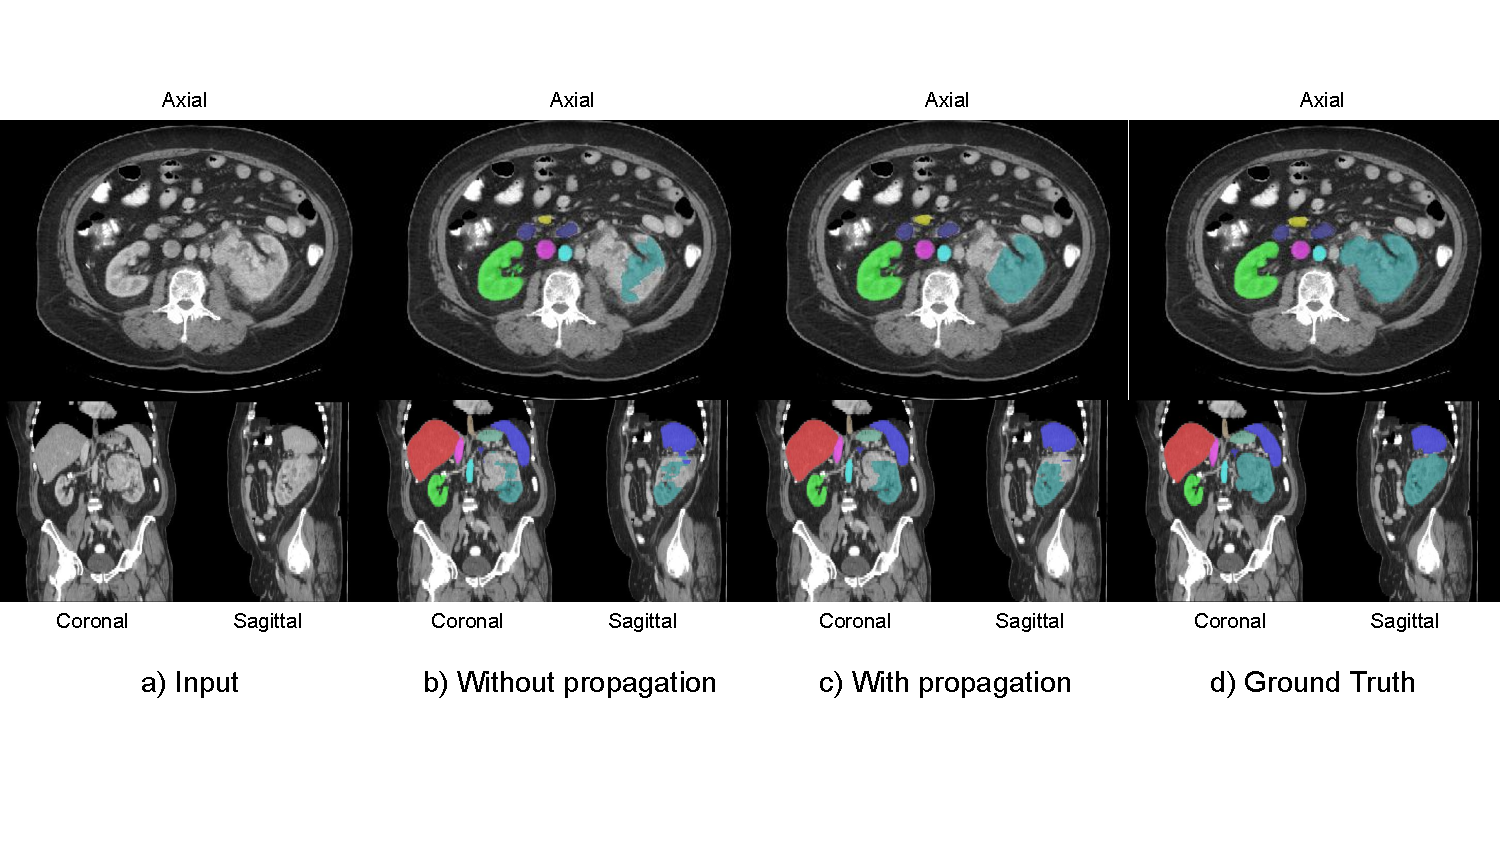
\includegraphics[width=\textwidth]{content/resources/new_images/qualitative/stcn_improvement.pdf}
\caption{Qualitative comparison between before and after mask-propagated refinement.}
\label{fig:stcn}
\end{figure}

\begin{figure}[!h]
\centering
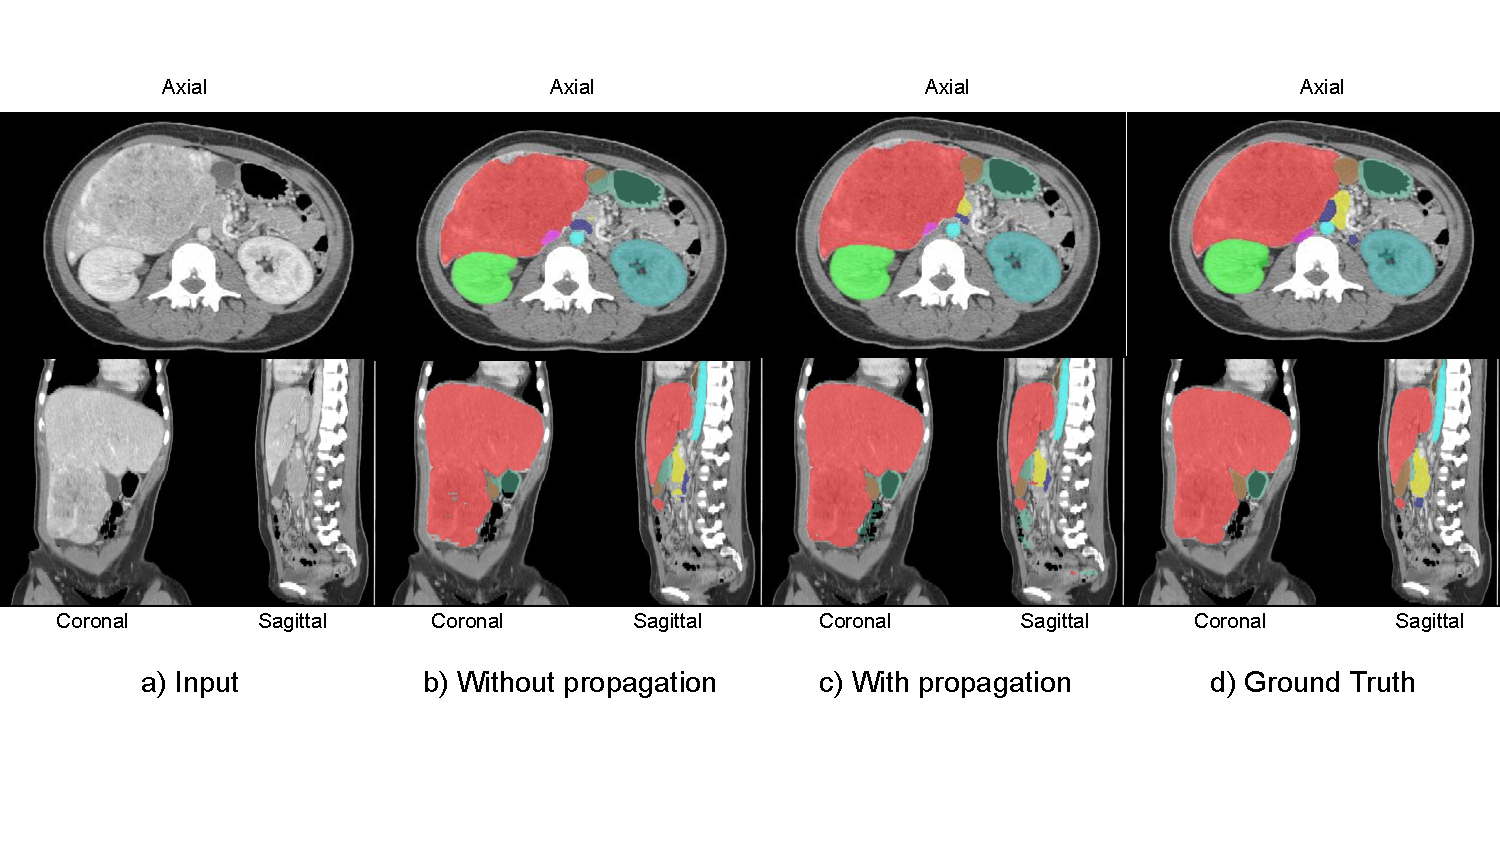
\includegraphics[width=\textwidth]{content/resources/new_images/qualitative/stcn_improvement2.pdf}
\caption{Another qualitative comparison between before and after mask-propagated refinement }
\label{fig:stcn2}
\end{figure}

Figure \ref{fig:stcn} and Figure \ref{fig:stcn2} showcases the refinement results of our proposed Propagation module. It can be recognized that the "Without propagation" columns represent the output masks of the Reference stage only.  We can see that with the second stage applied, some organ masks become smoother and more precise along the coronal and sagittal axis (the left kidney in Figure \ref{fig:stcn} and both the gallbladder, pancreas in Figure \ref{fig:stcn2}).

While the masks from the first stage are usually inconsistent along the temporal dimension, even between two consecutive frames, the Mask Propagation algorithm helps to stabilize the differences between them.

\subsection{Improvement of Cross Pseudo Supervision}

\begin{figure}[!h]
\centering
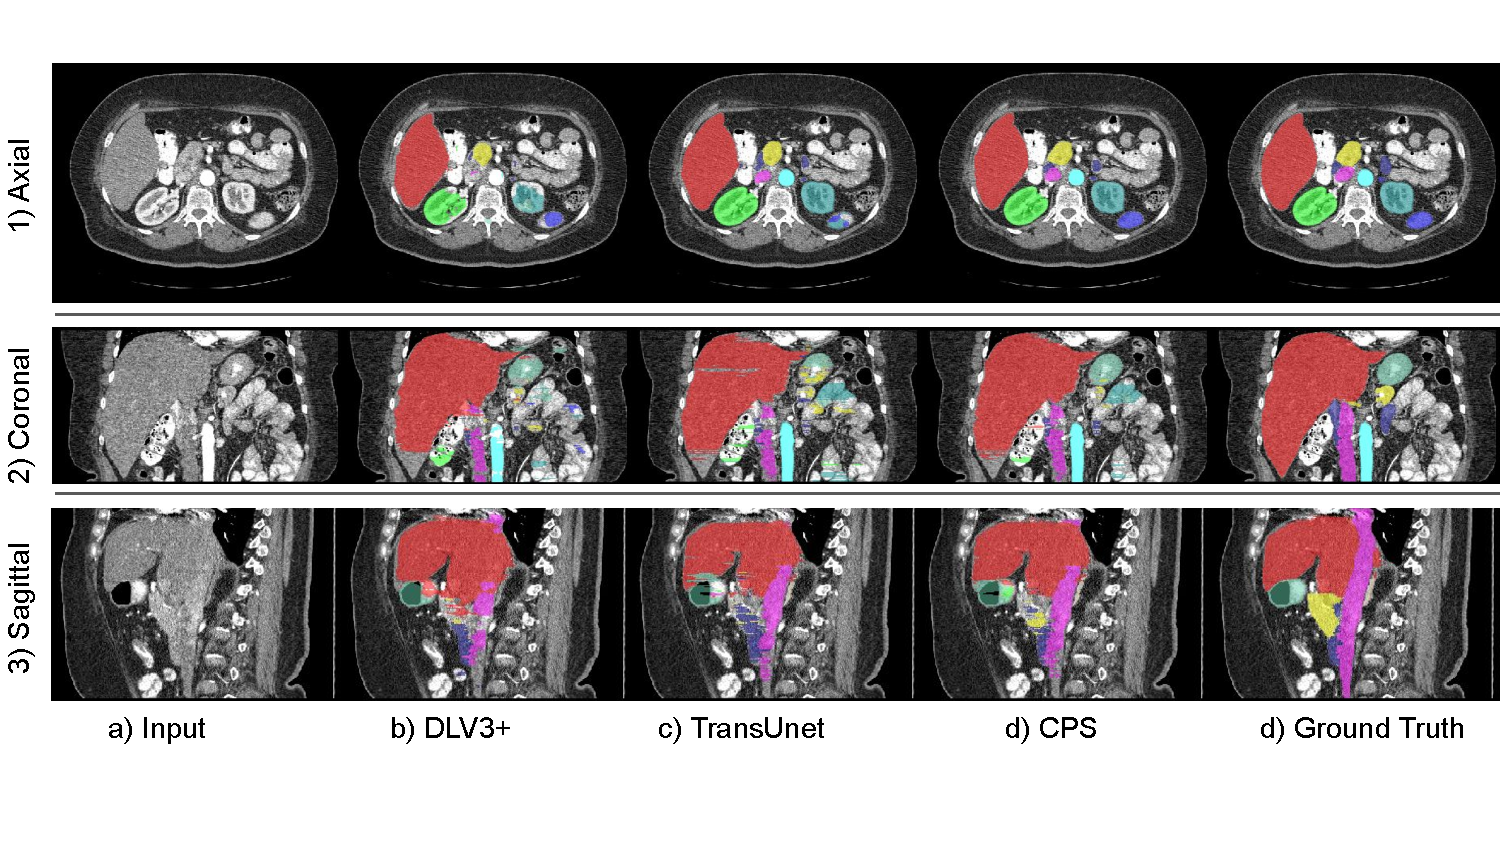
\includegraphics[width=\textwidth]{content/resources/new_images/qualitative/cps.pdf}
\caption{Comparison between before and after using Cross Pseudo Supervision in the Reference stage}
\label{fig:cps_improvement}
\end{figure}

The effectiveness of using CPS can be seen in Figure \ref{fig:cps_improvement}. It seems that the DeeplabV3+ and the TransUnet suffer from segmenting some different specific organs with small areas. CPS, on the other hand, gives more stable results (the small part of the spleen in the bottom right in the axial view, or the reduction in inconsistency along the sagittal plane, both in Figure \ref{fig:cps_improvement}).

\subsection{Improvement of Positional Encoding}

\begin{figure}[!h]
\centering
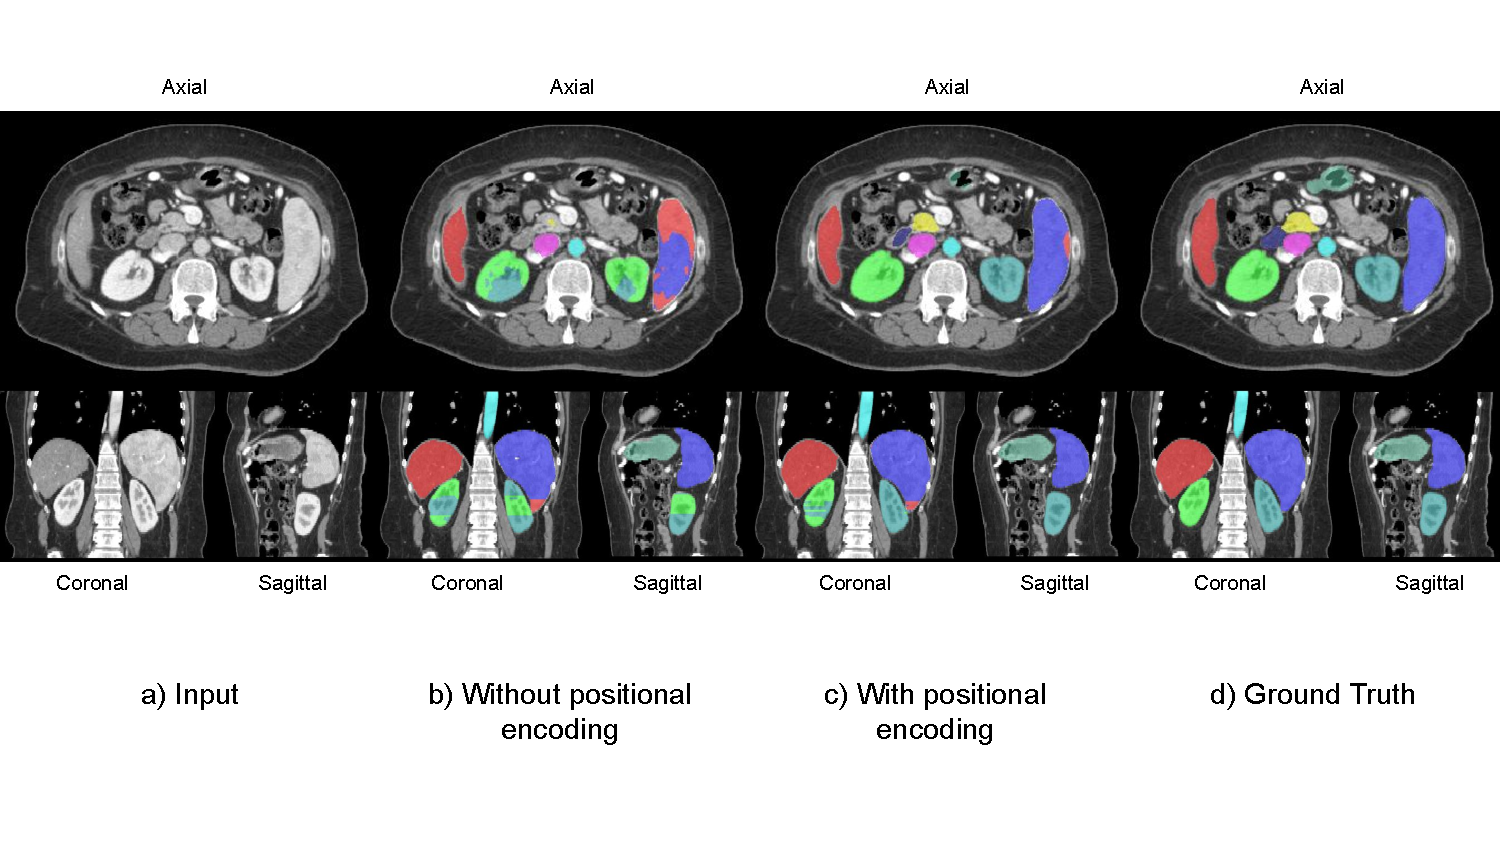
\includegraphics[width=\textwidth]{content/resources/new_images/qualitative/positional_encoding.pdf}
\caption{Comparison between before and after integrating positional encoding into the TransUnet in the Reference stage}
\label{fig:pe_improvement}
\end{figure}

The positional encoding includes the temporal information in the input of the Reference module. Therefore, it is expected to reduce the discordance between the sequence of slices. For example, the right kidney in Figure \ref{fig:pe_improvement} b), viewed in coronal and sagittal, is constantly mistaken for the right kidney. With the introduction of positional information, it is segmented accordingly. Moreover, it also accurately identifies the location of the pancreas and the left adrenal gland.


\subsection{Improvement of Pseudo Labeling with Uncertainty Estimation}

\begin{figure}[!h]
\centering
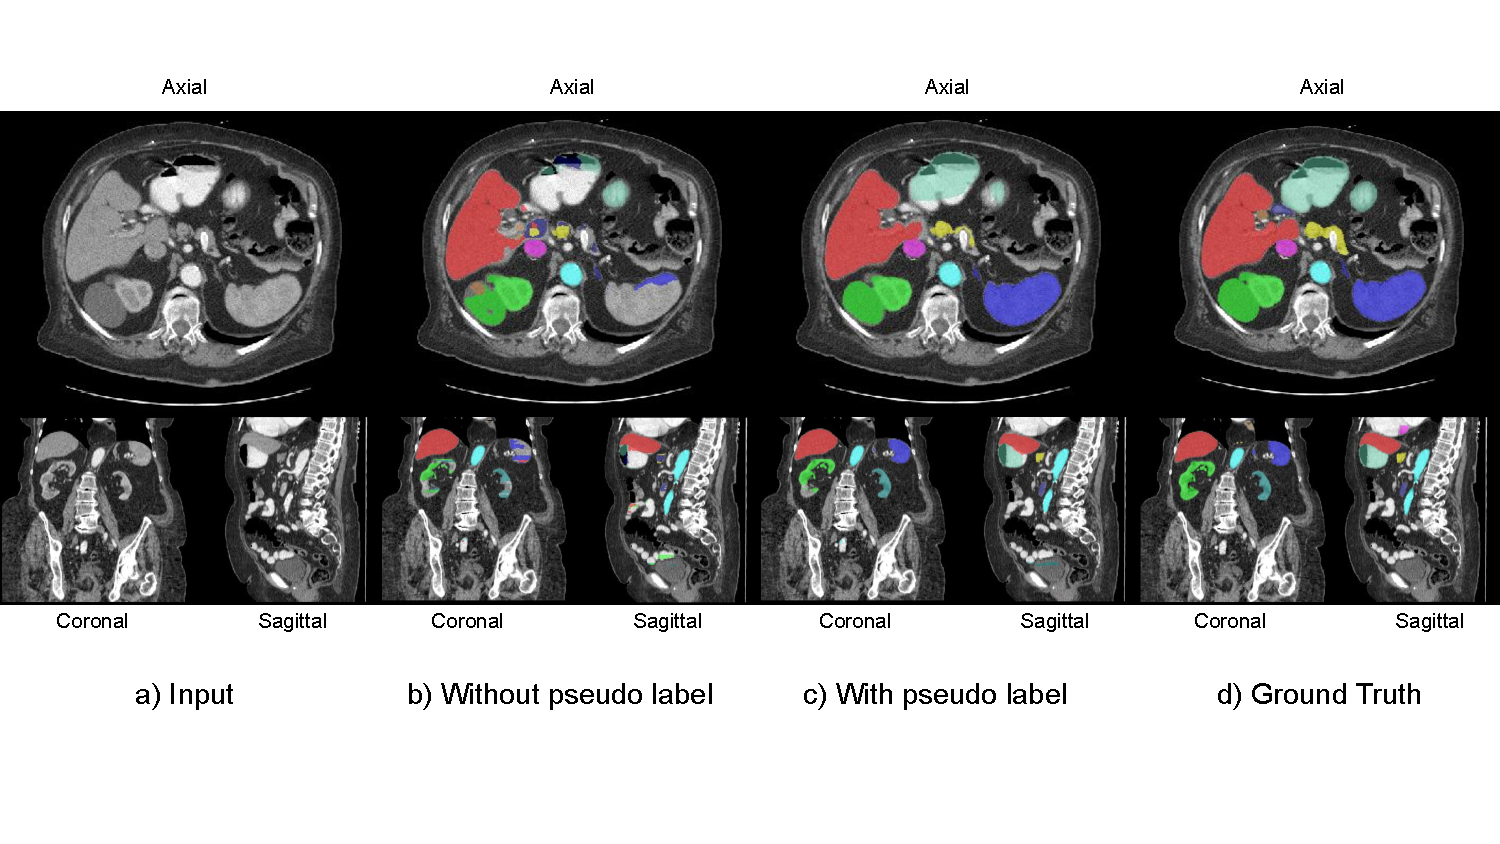
\includegraphics[width=\textwidth]{content/resources/new_images/qualitative/pseudo_labeling.pdf}
\caption{Comparison between before using pseudo labeling and after retraining the model with pseudo labeling}
\label{fig:pseudo_labeling_improvement}
\end{figure}

It is clear that the contribution of pseudo-labeling is significant to our final results. In Figure \ref{fig:pseudo_labeling_improvement}, most of the organ masks are notably enhanced after retraining with pseudo labels. However, we still have yet to resolve the imbalanced problem, which leads to the difficulty in identifying small organs like the gallbladder in the Figure. 


% \chapter{Application}
\label{chap-application}
\begin{ChapAbstract}
In this chapter, we present the implemented application of our proposed method for interactive video volume segmentation, including a annotation tool. 
\end{ChapAbstract}

\section{Overview}
\label{sec:overview}

\subsection{A brief introduction to Information Retrieval and the merits of Video-Text Retrieval}
%  paragraph 1
In recent years, we are witnessing impressive growth in both computer hardware and software, which have contributed to the outcomes’ improvement of many expensive tasks, including search.
Information Retrieval (IR), or search in common, is a long-history task claimed to appear in the third century BC in an early type relevant to library administration \cite{eliot2009companion}.
What people know of this terminology today is usually related to electronic devices and the Internet. For example, we may seek a friend’s name in a phonebook or look for a song from its lyrics, a movie from its content by using some search engines.
When we do not know something, instead of going to the library or any kind of information center like we did in the past, most of us constantly “google” it at first.
All of those examples, in fact, are associated with something called Information Retrieval System (IRS) - the implementation of any specific IR theory into the computer operation.
An IR system feeds a query in a particular type as input and gives back the most relevant results to the user through automatic matching methods between the input and data sources (see figure \ref{fig:IR_structure}).
\begin{figure}[!t]
    \centering
    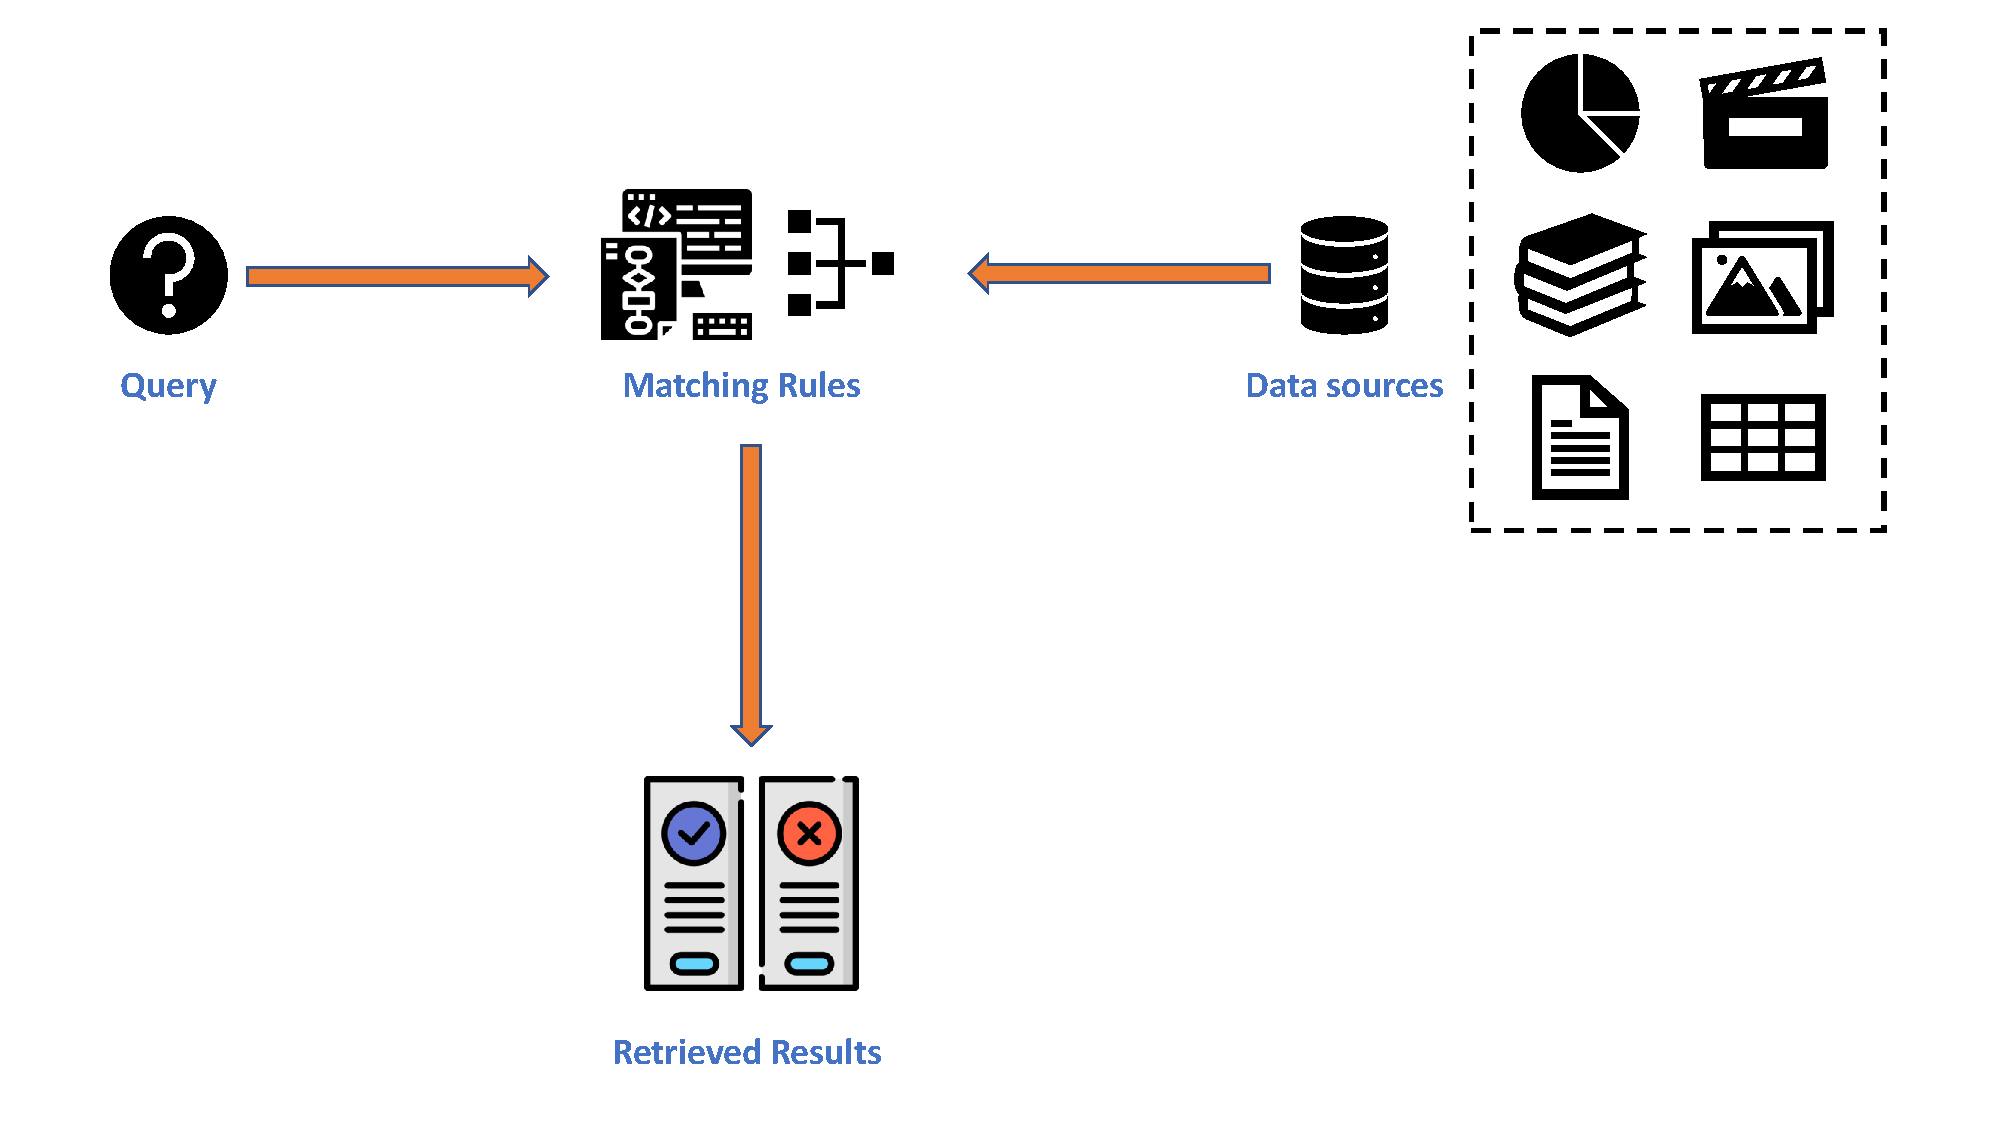
\includegraphics[width=\linewidth]{resources/images/overview/IR_structure.pdf}
    \caption{A simple overview of the Information Retrieval System}
    \label{fig:IR_structure}
\end{figure}
The need for such things occurred due to the increasingly rapid rise in data size and various kinds of information in different areas (like multimedia, website, scientific publication, etc.), making traditional searching techniques no longer cope.
In any IRS, there are always two aspects to deal with: system operation and matching algorithms. Since the first application in the 1940s, it has been developed continuously until now, with many essential milestones \cite{sanderson2012history} tackling both aspects.

%  paragraph 2
As the computing environment changes from time to time, many applications of IR have been suggested, like search on social networks, desktop element search, or one research hotspot recently named cross-modal retrieval.
This task aims to pick out relevant data across different modalities, such as image-text, video-text, audio-text.
Maragos et al. \cite{maragos2008multimodal} stated two future challenges with multimodal applications, including (i) Natural access and high-level interaction with multimedia databases and (ii) Detecting, recognizing and interpreting objects, events and human behavior in multimedia videos by processing combined audio-video-text data.
This statement also reflects two aspects that people always deal with the IRS, as mentioned above.
In research, people may care more about the method aspect than the other.
Traditional methods with manually designed representations, features and matching functions lack the ability to tackle complex IR tasks like multimodal interaction when those tasks require a deeper understanding of document contents and the user information needed \cite{culpepper2018research}.
However, thanks to an ever-stronger influence of Deep Learning \cite{goodfellow2016deep,lecun2015deep} in the 2010s decade, many problems raised in this field have resulted in better performance, letting people expect a new generation of robust and intelligent cross-modal Information Retrieval Systems.

%  paragraph 3
Also, humans have recently witnessed a rapid explosion in the appearance of videos in many aspects of their daily lives.
We all know the potential of videos in entertainment, communication, data analysis, etc.
The rise of video-based online services like YouTube, Netflix, along with the traditional TV program, has inspired Computer Vision (CV) experts to pay more attention to this resource. Additionally, natural language (NL) is one of the most effective means to describe those video contents.
From this point of view, the task of searching videos via text queries, or video-text retrieval, in short, becomes a desirable function in intelligent systems.
This problem takes (a) natural language text description(s) as input and outputs a sorted list of videos in terms of semantic relevance.
A lot of neuron network-based methods, focusing on transforming text input and video’s particular contents into the same subspace and measuring their similarity, have worked efficiently.
However, each video retrieval task has its own specificities among the diversity of the visual world, besides some in-tackling challenges like the semantic gap between two modalities, lack of annotated video-caption, or complicated consideration of temporal information, making no universal utilization approach fit for all such retrieval problems.
Therefore, caption-to-video retrieval is still attracting researchers to resolve in different areas.

\subsection{A brief introduction to Intelligent Transportation/Traffic System and the merits of Vehicle-oriented Computer Vision Tasks}
%  paragraph 1
Transportation is a non-separable part of any country, playing an essential role in different aspects of our daily life.
Residents, governments, and businesses almost depend on it to access resources.
Therefore, the advent of Intelligent Transportation/Traffic System (ITS), a significant factor contributing to the concept of smart city and to the development of modern civilization, is inevitable.
The implementation of ITS is widely accepted and used in many countries today when the governments recognize (i) the rapid growth of the human population, (ii) high-speed urbanization, and (iii) increasing vehicle ownership.
Though there are multiple modes of transportation, the roadway is the most common route.
So this kind of system aims to address a wide range of road traffic issues via advanced technologies, solving at three main levels: society, the road administrator, and drivers.
By providing different modules centering around the people-vehicle-road relation, and other traffic objects, it helps improve the safety, efficiency,  and environmental friendliness of the transportation.

%  paragraph 2
In an ITS that inherits Deep Learning works, Fan et al. \cite{fan2020deep} have shown that there are four major services in the architecture, as illustrated in figure \ref{fig:ITS_structure}.
\begin{figure}[!t]
    \centering
    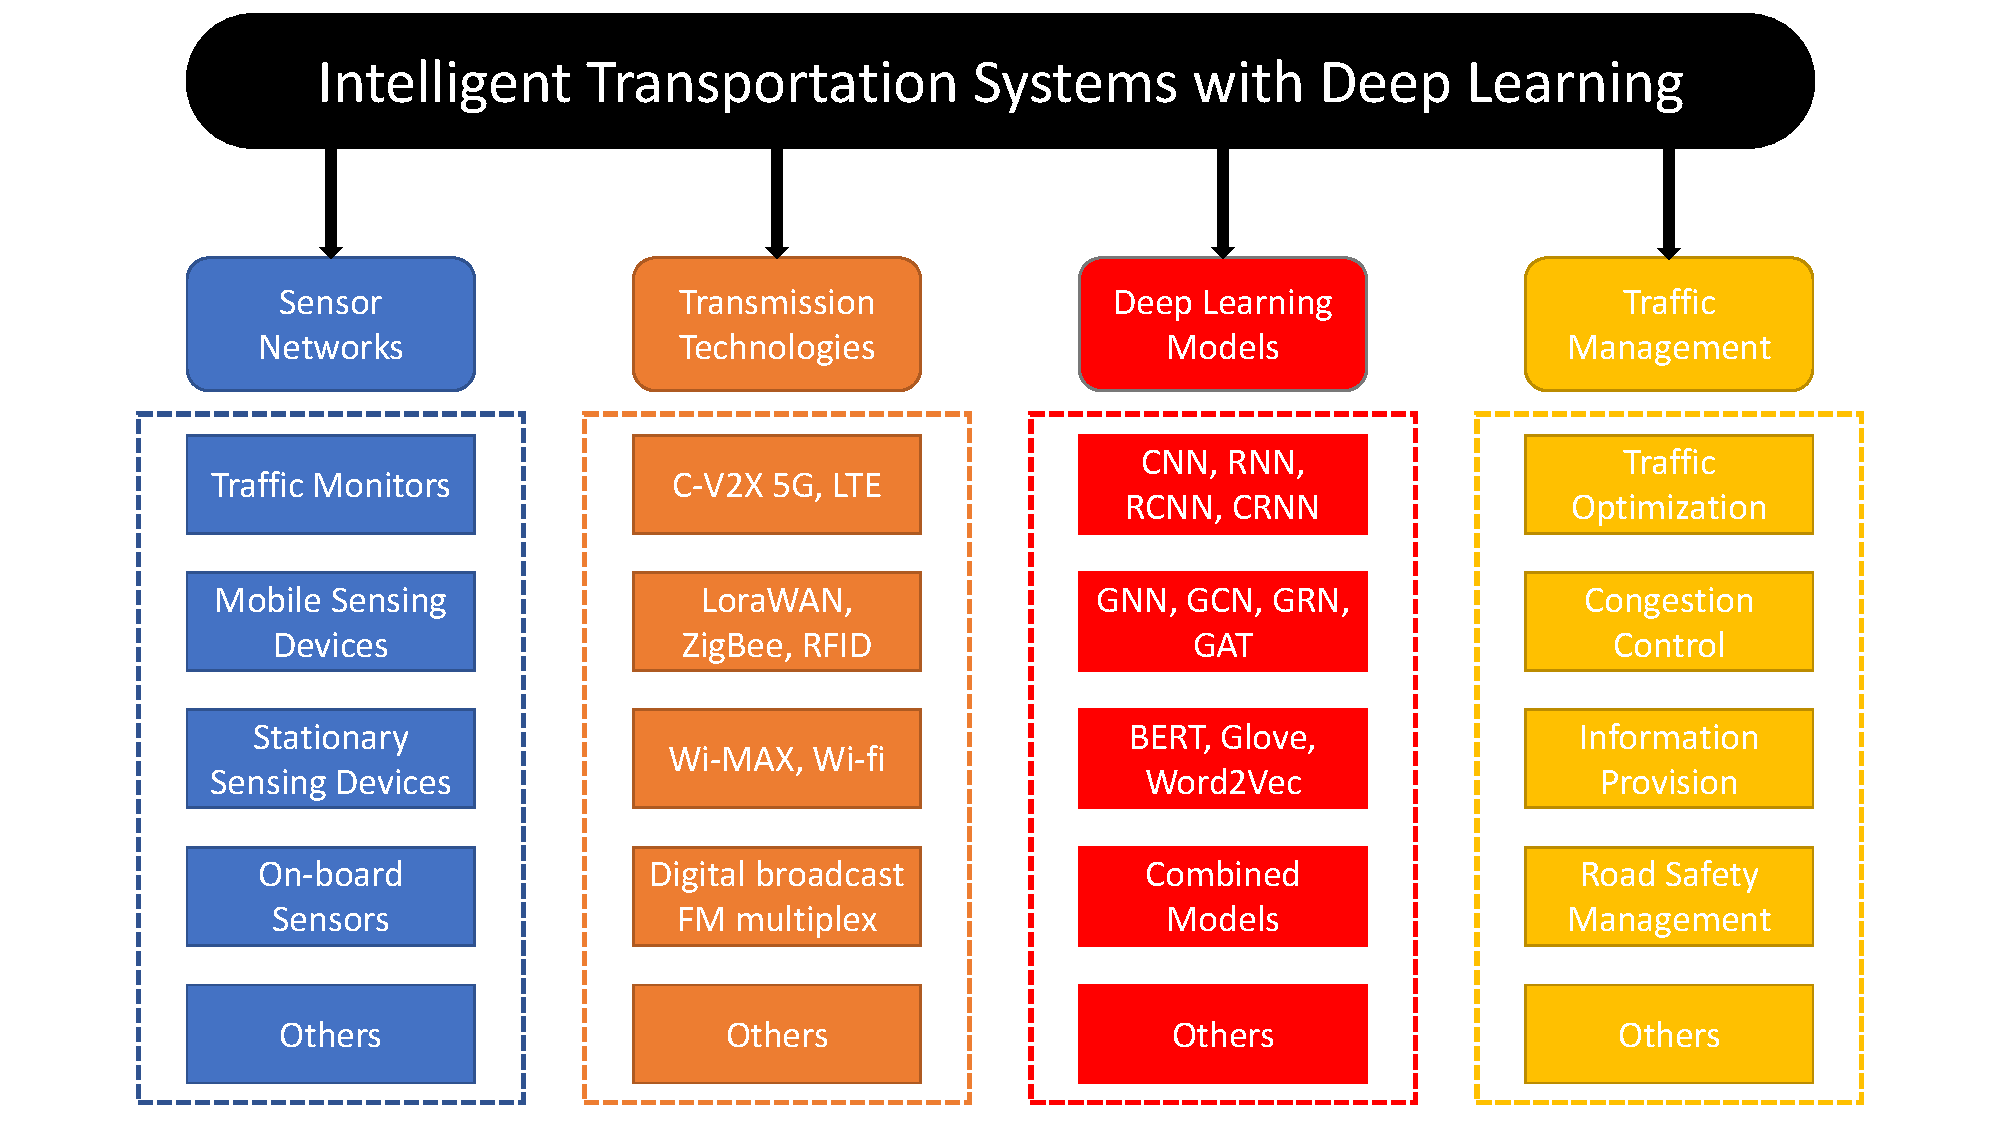
\includegraphics[width=\linewidth]{resources/images/overview/ITS_structure.pdf}
    \caption{Major components of a Deep Learning-based Intelligent Transportation/Traffic System.}
    \label{fig:ITS_structure}
\end{figure}
The Sensor Networks service is in charge of collecting real-time data then sends it through the Transmission Technologies service.
By exploiting the data, the Deep Learning Models service is responsible for building models that can perform well in particular tasks before integrating them into practical modules of the Traffic Management service.
When it comes to Computer Vision applications in such systems, many problems are mainly related to vehicles.
This is because transportation is vehicle-centered, unlike other areas, which are often people-focused.
Thanks to the widespread installment of 24/7 surveillance cameras on roads and highways, people can obtain massive traffic data.
Although the potential for video analytics from that data is enormous to be leveraged, it has not been exploited optimally.
Some tasks have received high-accurate state-of-the-art results, such as Vehicle Counting \cite{lu2021robust, dai2019video, asha2018vehicle} or Vehicle Reidentification \cite{luo2021empirical, Khorramshahi_2019_ICCV, zhu2019vehicle}, but some are still far from saturated outcomes.
Two major hurdles include the insufficiency of labels and the lack of high-performance models capable of converting data into valuable insights.
Regarding the model, since the vehicle is a particular domain and non-human, many pre-trained models cannot be applied directly to this object.
Therefore, CV researchers in this field still face so many significant challenges.
And, there should be something that can attract attention to address such issues.

%  paragraph 3
For those reasons, in parallel with the works of individuals, there are also organizations holding vehicle-oriented contests in order to find solutions from talented candidates.
Not stopping there, through these contests, people hope for deployments of submitted models into a realistic environment. 
One of the hottest contests is the AI City Challenge \cite{Naphade17AIC17, Naphade18AIC18, Naphade19AIC19, Naphade20AIC20, Naphade21AIC21}, opening continuously since 2017.
This contest primarily focuses on accurate, robust, and efficient approaches, so the organizers provide relatively sufficient labeled datasets \cite{Feng21CityFlowNL, Tang19CityFlow, Yao20VehicleX} as well as the evaluation system.
Their problems range from the mentioned tasks above to others like Velocity Estimation, Anomaly Detection, Vehicle Tracking, etc., whose insights may be inspired by various techniques.
In the latest edition, the 5th AI City Challenge \cite{Naphade21AIC21} has proposed a novel advanced track named Natural Language-Based Vehicle Retrieval (NL-based VR), which needs an effective combination of subtasks including motion detection, appearance recognition and content-based video retrieval.
There are still other tasks from other competitions, but finally, they all have the same goal: to solve real-world traffic issues and implement them into the Intelligent Transportation/Traffic System.
\subsection{Main features}
\begin{figure}[!h]
    \centering
    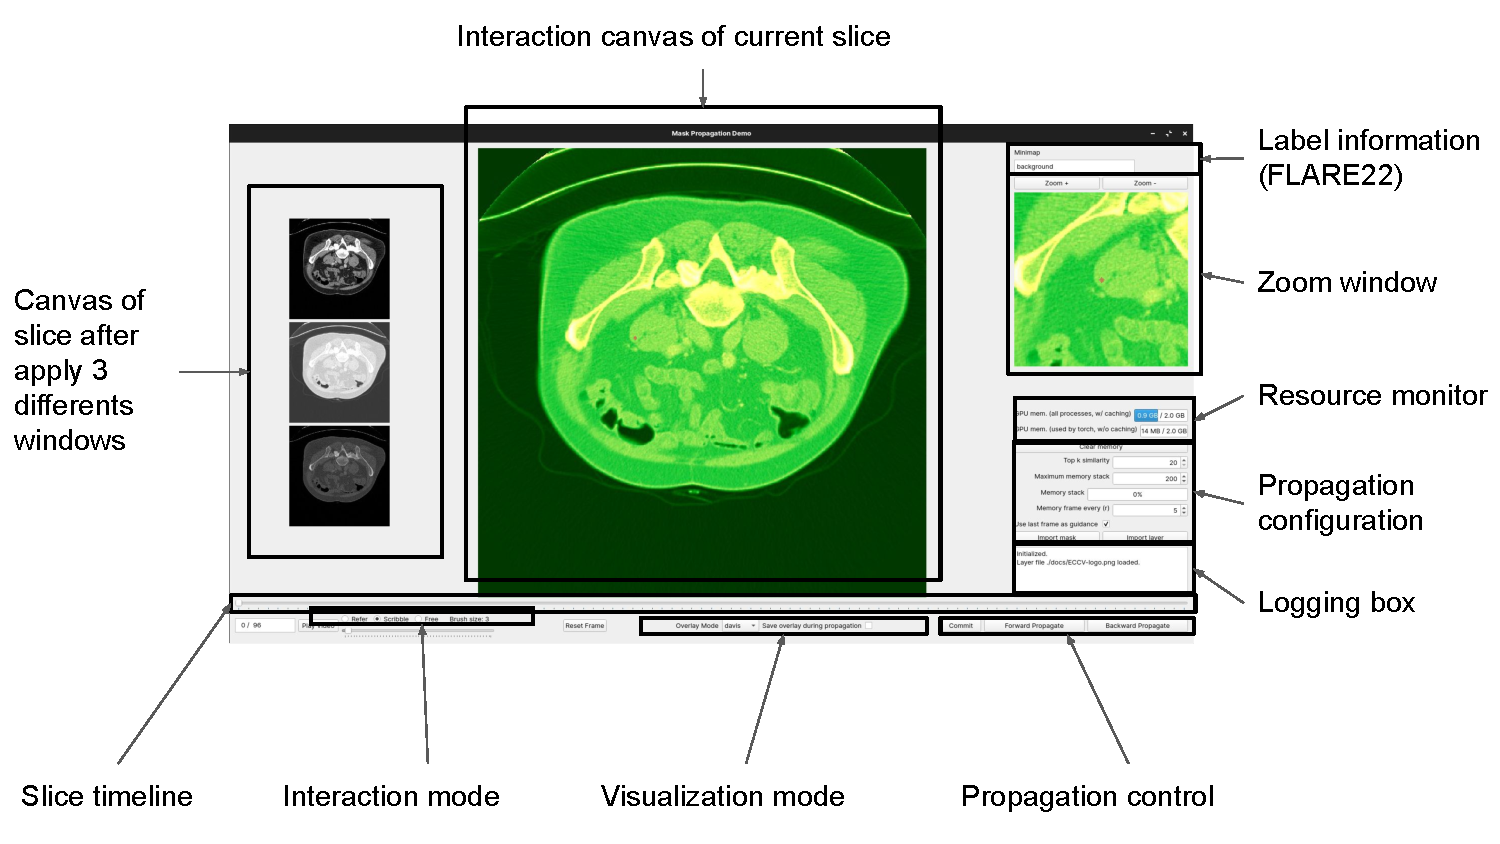
\includegraphics[width=\textwidth]{content/resources/new_images/application/GUI.pdf}
    \caption{The layout of our annotation tool}
    \label{fig:gui_app}
\end{figure}

% \textbf{Preview and select annotated slices}: 
% By using \textbf{slice timeline}, annotator can choose a arbitrary slice by dragging the slider. In each timestamp, two main canvas will be previewed corresponding: On the left side is the visualization of applied image on different window as we demonstrated before on section \ref{sec:preprocess}; The large main one is displays the concatenate image from 3 preprocessed image as a RGB image. The canvas on the right hand is the zooming window, increase the crop image size for small details interaction. The zoom in ratio could be modify by nearby zooming controller buttons, or maybe scroll wheel to zoom in and out.

% \textbf{The main controls include}: Using left and right mouse buttons for positive and negative clicks, or scribbles modify an existing mask respectively, press space to finish the current object; pressing the left arrow key displays the previous image, and pressing the right arrow key displays the next image, pause when correction is needed. Using the \textbf{propagation control} to propagate through the whole volume. The target object must be selected by using the number keys. "1" corresponds to the first object, etc. 

% \textbf{The monitors}: Stats would be printed on the logging box. The resource monitor also displays the GPU memory exists. Label information would be on the top right shows the information of hovering object.

% \textbf{The interactions}: We provide 3 type of interactions including: scribbles to mask, free scribbles and reference. 

\textbf{Selecting and previewing the annotated slices}: 
By using the \textbf{slice timeline}, the annotator can choose any arbitrary slice just by dragging the slider. In each timestamp, two main canvas are shown: on the left side is the visualization of applied image on different windows due to the aforementioned pre-processing stage (as in \ref{sec:preprocess}); The larger canvas in the middle displays the stacked version of the 3 images as a RGB image. 
We also provide the user with an additional canvas on the left side, which illustrates the zooming view of the main canvas for small details interaction. The zoom-in ratio could be modified by available controller buttons, or by scrolling the mouse wheel.Users can also navigate through the timeline by pressing the left arrow key and the right arrow key. 

\textbf{Performing slice annotation}: 
We provide 3 type of annotation interactions including: scribbles to mask (s2m), free scribbles and automatic reference. In the free scribble mode, the user can freely draw on the canvas to create object masks. Meanwhile, The s2m and reference options offer the ability to use deep learning models to automatically generate the masks. 
% Options are demonstrated in the \textbf{interaction mode}. 
The list of available objects can be shown by pressing "L". Then to choose a specific object that the user desire to label, corresponding keypad should be pressed. For example, to annotate an object that belongs to class "1", keypad "1" should be pressed. In both the scribbles modes, the user can use left and right mouse buttons to draw new masks or to erase existing masks respectively. After finishing, the user can press space to obtain the mask. With the initial mask formed, the user can perform forward/backward propagation to disseminate the annotated mask to other slices across the timeline. The \textbf{propagation control} provides options to accomplish that.

\textbf{The monitors}: Stats are printed in the \textbf{logging box}. The \textbf{resource monitor} also displays the current usage of GPU memory. Label information is also shown on the top right, indicating the information of the  object that is being hovered on.
\subsection{Annotation flow}
\begin{figure}[h]
    \centering
    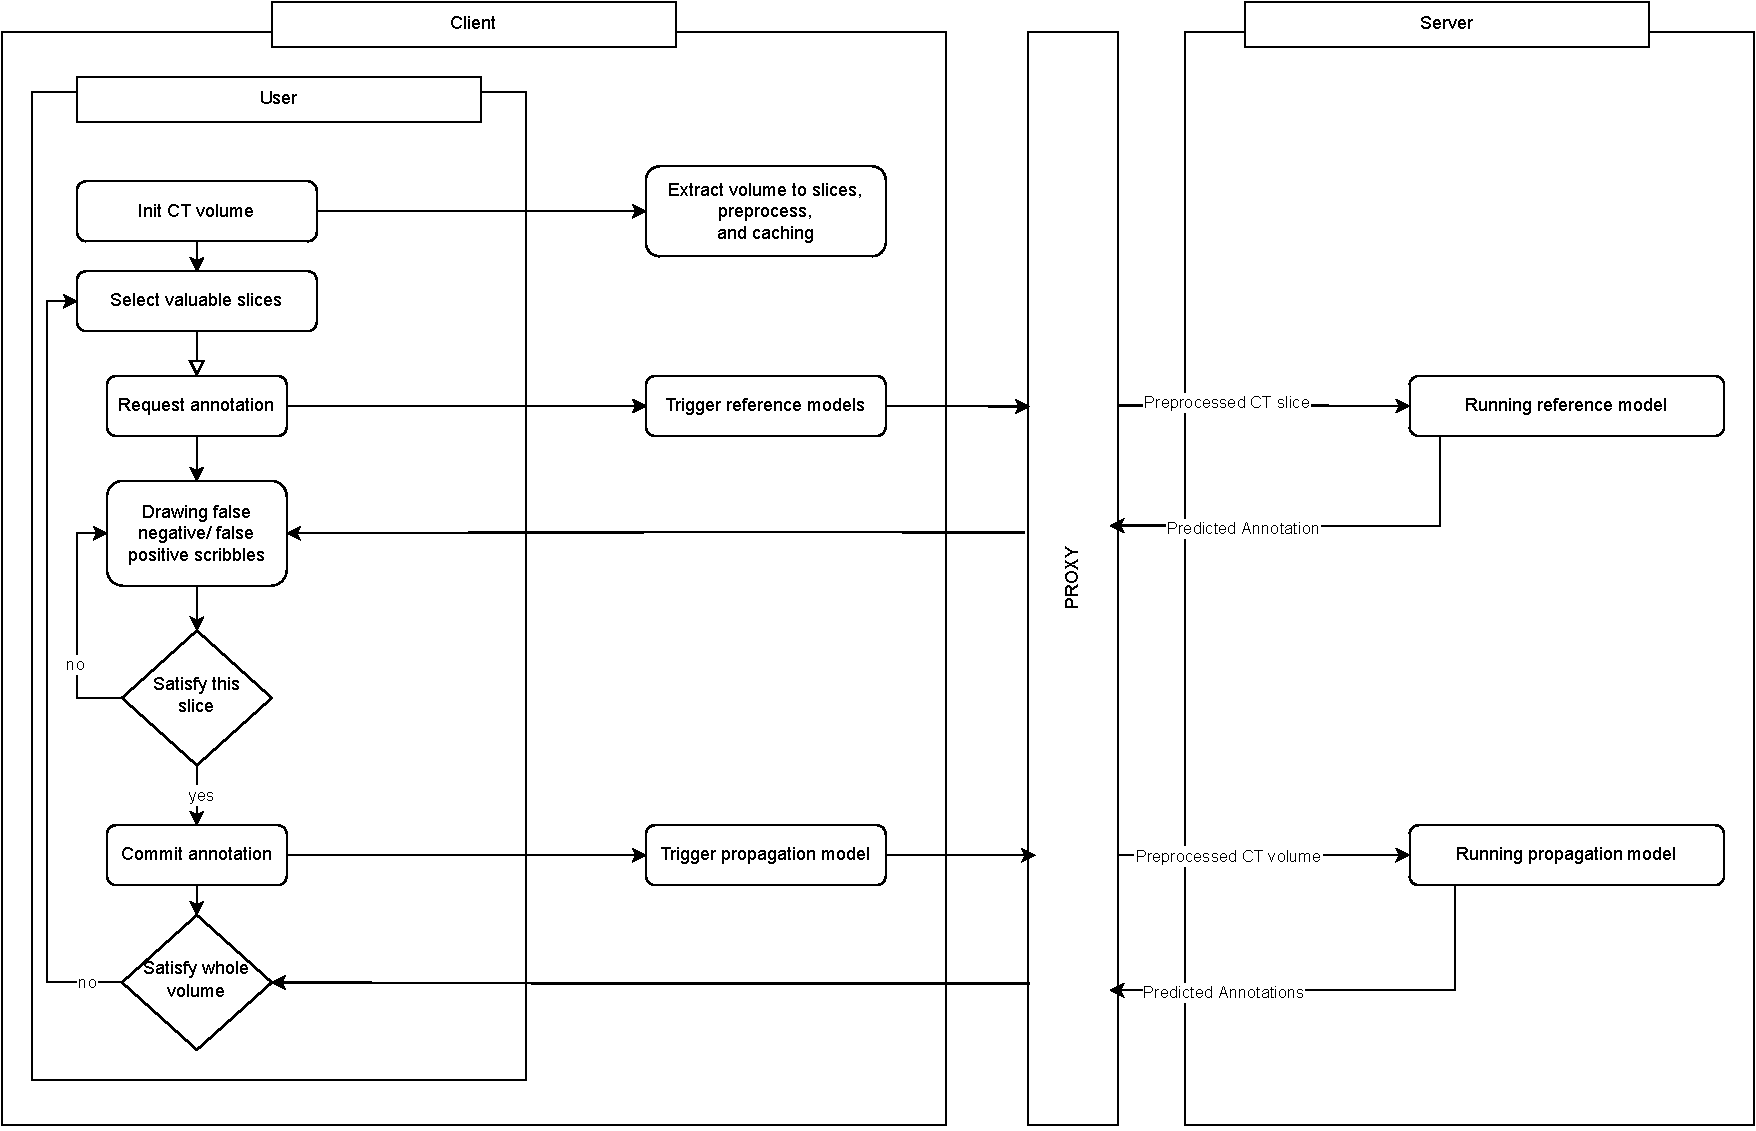
\includegraphics[width=\textwidth]{content/resources/new_images/application/Annotation_flow.pdf}
    \caption{The annotation flow for a CT volume}
    \label{fig:anno_flow}
\end{figure}
The annotation flow in Figure \ref{fig:anno_flow} shown in the diagram illustrates how users, clients, and servers interact with the other. After initialization, the annotator will select valuable slices for the refinement stage. The client will then wrap these slices and send them to the server. The request and response process will be communicated through a proxy. After the server has done its prediction on the whole volume image based on annotations from the refinements made by the annotator, this process will repeat until an acceptable level of results is achieved.

\subsubsection{Request parsing}
The serialization and deserialization processes is very important when it comes to exchanging data between the client and server. By using request parsing, we are able to use JSON for both the client and server messages. This makes the process quick and easy, while also ensuring that all of the data is properly transferred. There are some basic types that can be easily jsonified, such as numbers and strings. However, images and masks need to be encoded using the latin-1 encoder in order to ensure successful transmission.
\subsection{Future works}

In the thesis range, the application tool is not strictly required, but the system design must be flexible and scalable. Our implementation satisfies preliminary targets, but there are many points that can still be improved. For example, data management, cloud storing or  transferring process optimization can all be enhanced through caching or similar techniques.
% \chapter{Conclusion}
\label{chap-conclusion}
\begin{ChapAbstract}

In this chapter, we report the results and discuss about the future works for improving our proposed method and its applications. In our thesis, we proposed a novel pipeline to tackle the problem of CT volume organ segmentation along with an interactive tool that can help labeling process become less complicated. Overall, through ablation study, our method shows improvements over the original baseline, yet still have weaknesses. If these shortcomings can be resolved, we believe it can bring many breakthrough for both the deep leaning and medical fields. Having said that, it is left for the future works. 

\end{ChapAbstract}

\section{Results}

With new advancements in technology, there are endless possibilities for what can be achieved. In the medical field, one of the most common problems that doctors face is accurately segmenting 3D objects from 2D images or volume sequences. We propose a novel two-stage pipeline that can leverage the strength of many state-of-the-art 2D deep learning algorithms and techniques in videos and images, into the task of 3D object segmentation. This proposal aims to introduce a novel and inspirational approach to solving one of the most common problems in the medical field. In addition, to break the barrier of differences in medical pipeline processes, our solution is able to transfer and exploit the power of multiple domain data to create more accurate results.

In summary, we enhance the initial results by presenting the application of new techniques and modules:

\begin{itemize}
    \item The semi-supervised Cross Pseudo Supervision module helps to exploit the enormous amount of unlabeled data successfully. According to our ablation study, with the usage of only a quarter of the unlabeled source, the validation results were boosted significantly. Additionally, this module also contributes to the pseudo-labeling stage to generate more data for other module to learn.
    
    \item The Propagation module which inherit the power of STCN model with some modification for adaptation. By using this module, the initial results were refined to obtain better masks. This module can also be attached to the annotation tool with ease and efficiency. However, its performance is strictly dependent on the precision of the previous stage, which is the Reference module. 
    
    \item The rational uncertainty estimation approach for the pseudo-labeling process, which helps the process becomes more explainable and productive. Despite that, its simplicity allows it to be further analyzed and upgraded in the future.  

\end{itemize}

On top of that, we also come up with a user-friendly annotation tool that provides support and guidance for doctor to quickly generate usable data for the medical field. 

Although our research shows improvements over traditional 2D methods, it still cannot be comparable to other 3D methods, as can be seen on the leaderboard of FLARE22 challenge, since those methods can comprehend the dimensional information of a full CT volume. Officially, our method achieves the final result of 0.78 DSC. Still, our method does introduce a novel approach yet promising one and can be further developed in the future.
\section{Future works}

It is undouted that there is a lot of space for our method to improve. Although it is more resource-efficient than the original method, it requires huge memory bank to store information during the testing phase. There have been many recent research with solution to alleviate this problem by using multiple memory storage mechanism \cite{cheng2022xmem}, or an identity assignment bank to associate multiple objects at once \cite{yang2022associating}. Unfortunately, at the time they are introduced, we have nearly come to the end of our thesis. It would be highly recommended for readers to look into these research.

Some drawback of the model comes from the unique property of the dataset, however we lack of expert knowledge to carefully look at those error case by case. It is encouraged in the future for researchers to perform in-depth investigation to obtain more valuable insights.

\import{chapters}{chap-introduction}
\import{chapters}{chap-background}
\import{chapters}{chap-related-works}
\import{chapters}{chap-method}
\import{chapters}{chap-experiment}
\import{chapters}{chap-application}
\import{chapters}{chap-conclusion}
% % For eureka submission
% \include{chap-intro-eureka}
% \chapter{Background}
\label{chap-background}
\begin{ChapAbstract}
In this chapter, we discuss all necessary background knowledge related to our work. First of all, we start with the very beginning concept in machine learning and then introduce some fundamental models used in processing complex data such as time-series or digital images. Then we introduce a list of Computer Vision problems which play an important role in our proposed approach. 
\end{ChapAbstract}


\section{CT Volume Image}
% ref https://www.ncbi.nlm.nih.gov/books/NBK574548/
CT images are two-dimensional pictures that represent three-dimensional physical objects. The images are made by converting electrical energy (moving electrons) into X-ray photons, passing the photons through an object, and then converting the measured photons back into electrons. The number of X-rays that pass through the object is inversely proportional to the density of the object. Objects imaged by CT consist of parts that vary in density. 

Image slices can either be displayed individually or stacked together by the computer to generate a 3D image of the patient that shows the skeleton, organs, and tissues as well as any abnormalities the physician is trying to identify. This method has many advantages make doctors easier to find the exact place where a problem may be located or identification of basic structures as well as possible tumors or abnormalities.

\subsection{Digital image representation}
% - how the computer store the images ?
In machine computing, image is a well-known definition. The image is construct by multiple pixels, each of them contains multiple values representing its visual information. The value range is often between from 0 to 255, for example it can handle the image brightness or the affect of a specific color (in a colored image). 
% insert image rgb 
Every image is define by structure information, such as image shape like channel, width, height. If the number of channel is 1, the image should be grayscale. And in color image, the number of channel would be 3 (corresponding with red, green and blue). And there are multiple variants of image type, like medical image shape would be constructed by width, height and depth. The depth channel could be thousand and pixel value range could be a negative number.
% insert volume image
\subsection{Hounsfield Units}
The CT detectors measure the degree that the scanned tissues physical density, and the image processor storing the data as pixels calculated by to convert byte data into a range of 5000 values. The scale's range of values is named for Hounsfield; each value on the scale is termed a Hounsfield unit (HU). Densities of various substances have been assigned relative values. The density of the substances in the patient (both natural tissues and any medical implants) and around the patient are calculated based on a linear transformation of the measured \textbf{X-ray attenuation coefficients}. This transformation is based on the standard density measurement of two substances, distilled water (set as 0 HU) and air (set as -1000 HU). HU for various scanned tissues are computed from the following equation: 
\begin{equation}
    HU = 1000 \times (tissue \mu - water \mu)/ water \mu 
\end{equation}
Where $\mu$ is the linear attenuation coefficient. CT scanners used in medical practice can present HU within a range of –1024 HU to +3071 HU. Different publications define different ranges for certain tissues and substances.

% Tissue physical density is proportional to photon attenuation (photon absorption). The CT detectors measure the degree that the scanned tissues attenuate photons (i.e., their density), and the image processor storing the data as bytes converts these values so that displayed pixels have proportionately assigned pixel brightness. A formula for this calculation to convert byte data into a range of 5000 values is used globally.[10][11] 

% The scale's range of values is named for Hounsfield; each value on the scale is termed a Hounsfield unit (HU). Densities of various substances have been assigned relative values, which are termed attenuation coefficients. The density of the substances in the patient (both natural tissues and any medical implants) and around the patient are calculated based on a linear transformation of the measured X-ray attenuation coefficients.[12] This transformation is based on the standard density measurement of two substances, distilled water (set as 0 HU) and air (set as -1000 HU) at 0 degrees Celsius temperature and a pressure of 10 Pascals.[13] HU for various scanned tissues are computed from the following equation: 

% HU =1000 X (tissue μ – water μ)/ water μ, where μ is the linear attenuation coefficient 
% CT scanners used in medical practice can present HU within a range of –1024 HU to +3071 HU.[14] Interpretation of clinical images often depends on evaluating a structure's HU, such as differentiating vascular lesions (which are dense when filled with contrast) from non-vascular lesions and distinguishing acute hemorrhage (which is dense) vs. non-acute hemorrhage or other substances. Different publications define different ranges for certain tissues and substances, for example: 


% \subsection{Image Windowing}

\section{Machine Learning and Deep Learning}
For the past decades, Machine Learning has become one of the most powerful tools, allowing individuals to perform complex analyses for better insights. The technique is widely applied and brings significant benefits in various vital fields, such as business, healthcare, agriculture or traffic management, etc.
Differ from the traditional programming paradigm, where the engineers have to craft the input data themselves and propose many rules to produce the most satisfying answers. \\
However, when the data increases extremely large, it contains many latent trends and patterns, which usually diminish hand-crafted solutions to get potential results.
This is where the Machine Learning techniques take place. The main goal of the approach is to develop a system that receives our observed data and corresponding expected answers, then return a set of rules that best fit those samples. These rules can be utilized to make predictions for new input. 
The machine-learning system applies some transformations on the input data to extract frequential or special patterns, which are usually called features, then use them to predict the output. The approach’s performance is then evaluated by appropriate metrics for the given task. Based on these scores, the system can choose the best transformation for each problem among a set of predefined functions (also known as hypothesis space). \\
As a subfield of machine learning, deep learning is formed as complex neural network architectures, containing more processing layers to learn hidden representations of the input data. 
This improvement is constructive in perceptual problems, where hand-crafted filters are merely impossible to achieve good results. 
In the following sections, we first discuss the beginning but original neural network to the further advanced ones.

\section{Deep Learning and Neural Network}
\label{model:mlp}

\subsection{Overview}
As a subfield of machine learning, deep learning is formed as complex neural network architectures, containing more processing layers to learn hidden representations of the input data. This improvement is constructive in perceptual problems, where hand-crafted filters are merely impossible to achieve good results. In the following sections, we discuss from the original neural network to the further advanced ones.

\subsection{Perceptron}

\begin{figure}[!h]
    \centering
    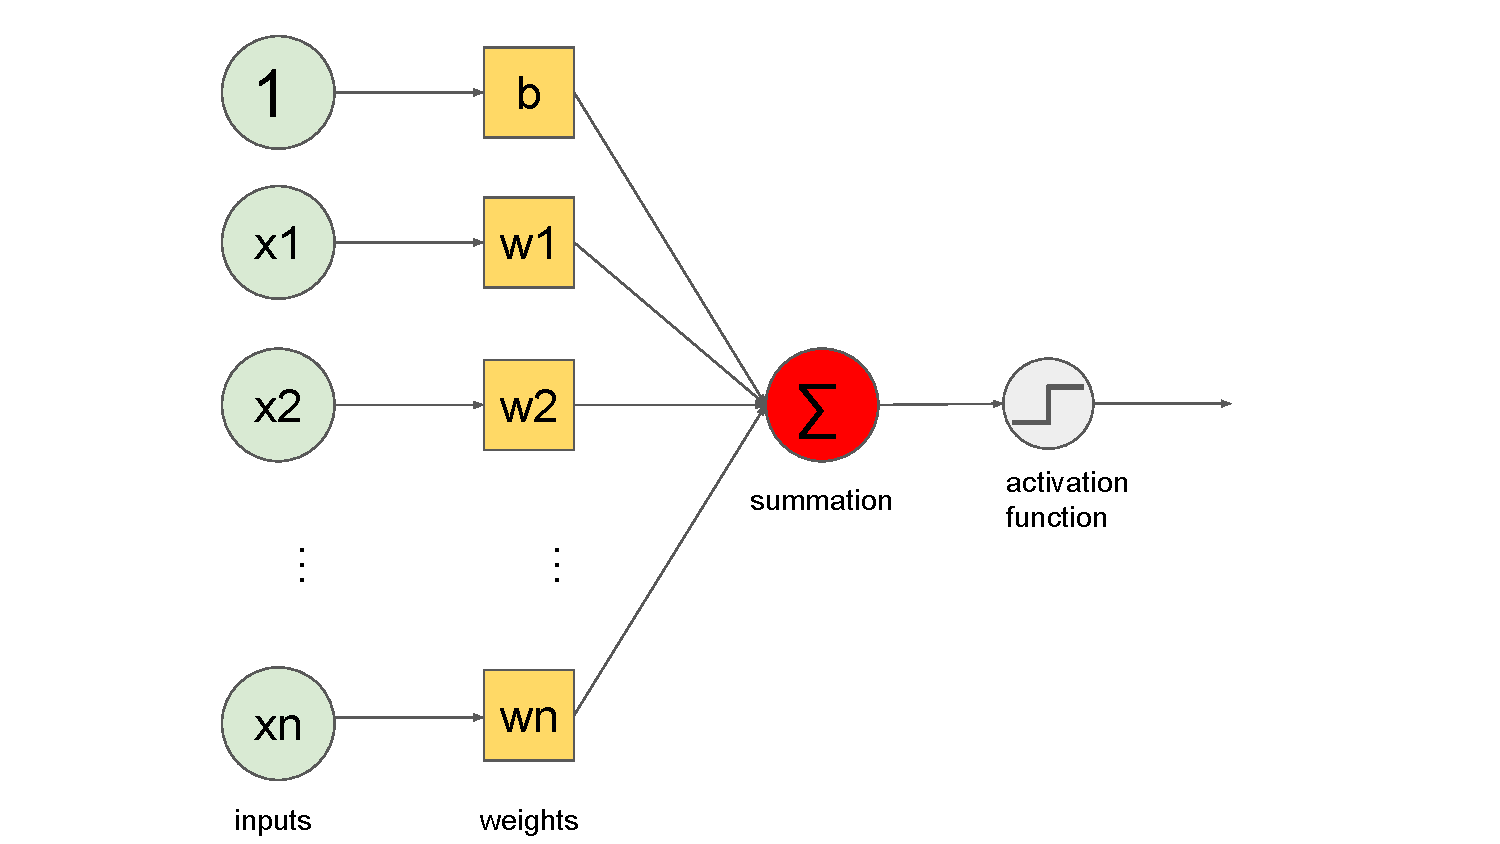
\includegraphics[width=\textwidth]{content/resources/new_images/related_works/perceptron.pdf}
    \caption{A single perceptron}
    \label{fig:perceptron}
\end{figure}

We first recap the early neural network, perceptron, which was introduced by Frank Rosenblatt in the 1950s \cite{rosenblatt1958perceptron} and 1960s \cite{rosenblatt1961principles}. 
The perceptron is an algorithm or a function for learning a binary classifier.
The function takes a $d$-dimensional vector $\mathbf{x}$ as input along with a weight vector $\mathbf{w}$ and calculates a single output value. 
\begin{align} \label{eqn: perceptron}
    a = f(\mathbf{x}) = \sigma(\mathbf{w}^T\mathbf{x} + b)
\end{align}
where $\mathbf{w}^T\mathbf{x} = \sum_{i=0}^{d} \omega_{i}x_{i} $ denotes the inner product between the input and weight vector and $b$ is bias. The perceptron behaves as a nonlinear function $\sigma$ of a linear combination of the input where each element $x_{i}$ is multiplied with it's corresponding coefficient $\omega_{i}$. 
Figure \ref{fig:perceptron} illustrates the process of a single perceptron process.\\
At first, the perceptron function is designed to solve the \textit{binary classification} problem in which each datapoint $\mathbf{x}$ belongs to a single class (denoted as \textbf{1} or \textbf{0}) and the weight vector $\mathbf{w}$ represents a boundary hyperplane that splits the space into two classes seperately. 
Therefore, points that lie at the same side of the plane are grouped to the same class. 
And the $sign$ function is used as activation function $\sigma$ in \ref{eqn: perceptron} to return $1$ if the combination is positive and $0$ otherwise.
\begin{align} \label{eqn: sgn_perceptron}
    a = f(\mathbf{x}) = \left\{\begin{matrix}
1 & \text{\quad if \quad} \mathbf{w}^T\mathbf{x} + b\geq 0 \\ 
0 & \text{\quad if \quad} \mathbf{w}^T\mathbf{x} + b <  0 
\end{matrix}\right.
\end{align}

\subsection{Activation functions}

Different from perceptron, activation function here is continuous, which makes the network weights differentiable with respect to output signals. \\
\begin{figure}[h]
    \centering
    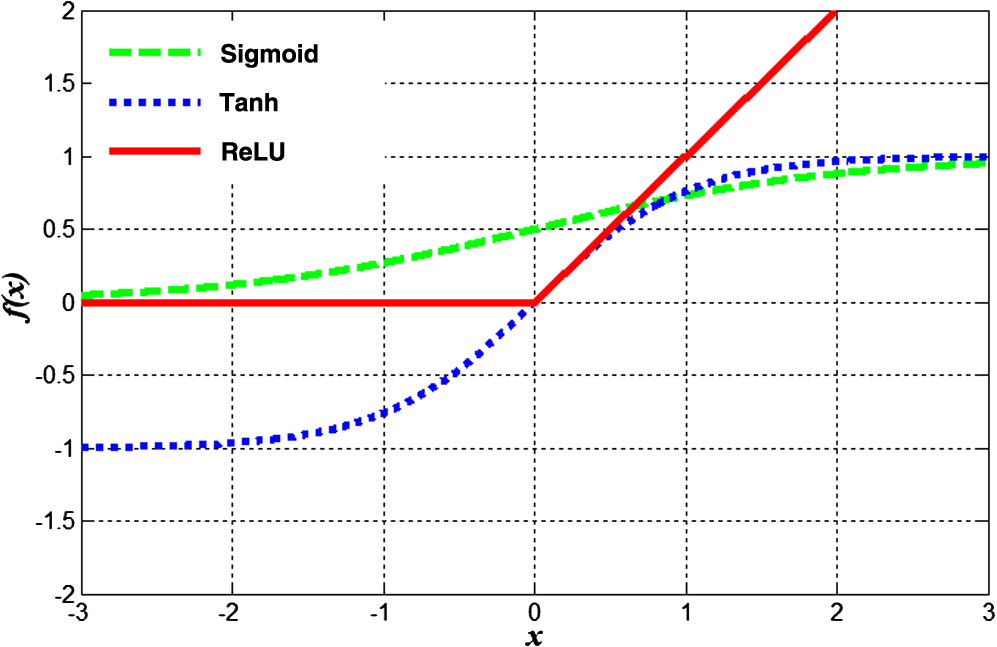
\includegraphics[width=0.7\textwidth]{resources/images/activation.png}
    \caption{Plot of Sigmoid, Tanh and ReLU activation functions.}
    \label{fig:activation}
\end{figure}
Here we list some of those activation functions commonly used in neural network modeling:
\begin{align} \label{eqn:sigmoid}
    \mathrm{sigmoid}(x) = \frac{1}{1 + \exp(-x)}
\end{align}
\begin{align} \label{eqn:tanh}
    \mathrm{tanh}(x) = \frac{\exp(2x - 1)}{\exp(2x + 1)} = 2 \times \mathrm{sigmoid}(2x) - 1
\end{align}
\begin{align} \label{eqn:relu}
    \mathrm{relu}(x) = \mathrm{max}(0, x)
\end{align}
The $sigmoid$ function (\ref{eqn:sigmoid}) scales real numbers to the range $[0, 1]$, where the large positive numbers change to $1$ and the large negative ones become $0$. Similar to $sigmoid$ but aims to produce zero-centered signals, $tanh$ function (\ref{eqn:tanh}) is a scaled version of $sigmoid$ with values range of $[-1, 1]$.\\
The drawback of both $sigmoid$ and $tanh$ is that when the numbers are large, the squashed values are saturated, hence their gradients is extremely small, which leads to the vanish problem when training deep neural networks. In such cases, Rectified Linear Unit ($ReLU$, \ref{eqn:relu}) is preferably used, which converts negative values to zero while keep the positive ones.
Figure \ref{fig:activation} illustrates the three functions in the same input range.



\subsection{Artificial Neural Networks}

The study of artificial neural networks (ANNs) has been inspired by the observation that biological learning systems are built of very complex webs of interconnected neurons in brains. The human brain contains a densely interconnected network of approximately trillion of neurons. ANN systems are motivated to capture this kind of highly parallel computation based on distributed representations. 

Generally, ANNs is a combination of a large number of interconnected processing neuron organized in a multi-layer architecture, where signal from a neuron can be passed to another from nearby layers (figure \ref{fig:neural_nets}). Each neuron is also formulated the same form as \ref{eqn: perceptron}. In general, neural network has an input layer, an output layer and a predefined number of hidden layers. Each hidden layer stands for a single transformation step in the process, which aims to extract hidden patterns of the input stored in it's neurons.  In recent years, state-of-the-art neural networks have multiple hidden layers. The number of layers determines the depth of the network, in contrast to the width of the network, which is determined by the maximum number of neurons between the hidden layers. In many cases, increasing depth increases the complexity of
the model, creates more space to store information and therefore increase its learning capability. These information is continually passed to following layers to extract more essential features. Due to the fact that sequence of linear transformations always equals to a single linear one, neural network uses nonlinear activation function $\sigma$ to element-wise apply to each processed neuron. 

\begin{figure}[h]
    \centering
    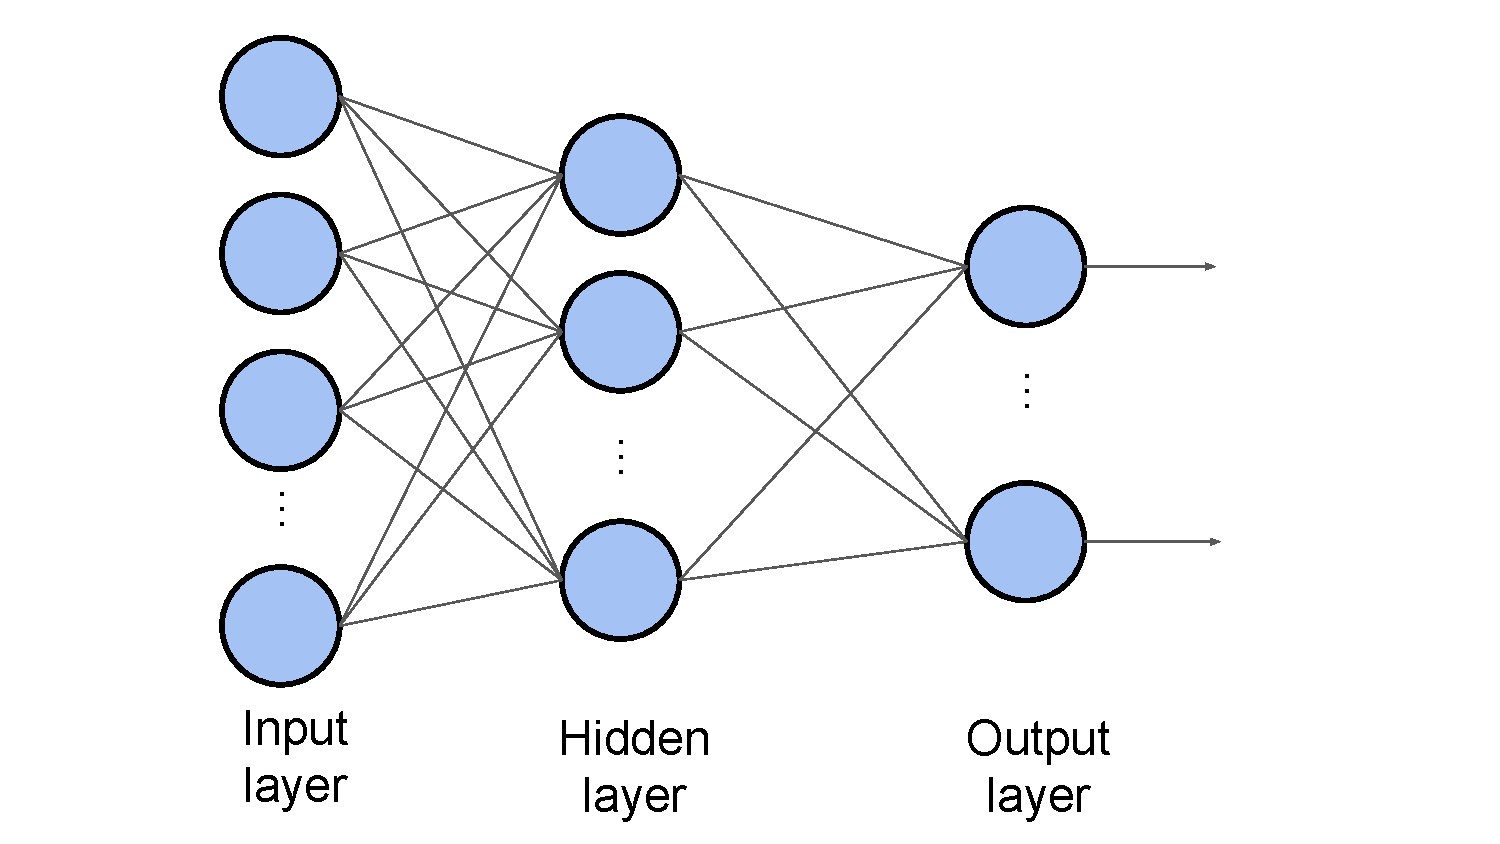
\includegraphics[width=0.7\textwidth]{content/resources/new_images/related_works/neural_nets.pdf}
    \caption{A simple three-layer neural network}
    \label{fig:neural_nets}
\end{figure}


Researchers have been actively conducting research on designing the architecture for ANNs to tackle machine learning and deep learning problem. Each new network design establishes on top of the older ones and each aims to solve a specific task independently. In order for the networks to deal with different tasks, such as classification, object detection, human action recognition, it cannot be without the usage of loss functions.

\subsection{Loss functions}

As stated in \ref{sec:ml}, supervised-learning neural networks must be trained with plenty of inputs-outputs data pairs. With every input, the network is expected to give a predictive outcome. While training, the network continuously adjusts its weights to minimize the discrepancy between its predicted outcome and the real outcome. The value of the discrepancy is often measured by using loss functions.

Loss functions are very diverse, each aims to solve different things and also is used for different tasks. For instance, in the regression task, the most used loss function is the least mean squared error. Suppose we have a model with parameters $\theta$, given a training sample $(x,y)$ where $x$ is the input and $y$ is the ground-truth, the loss for this single sample is calculated as follows

\begin{equation}
    \mathcal{L}(\theta,x,y) = \frac{1}{2} [y - h_{\theta}(x)]^2
\end{equation}

Similarly with classification task, the most frequently used one is cross-entropy loss. With the same notation as the example above, the loss function is as follows

\begin{equation}
    \mathcal{L}(\theta,x,y) = - (1-y_i) \text{log}(1-h_\theta(x_i)) - y_i\text{log}h_\theta(x_i)
\end{equation}

There are various factors involved in choosing a loss function for specific problem such as type of machine learning algorithm chosen, ease of calculating the derivatives and to some degree the percentage of outliers in the data set. 

So far, loss functions are used to determine the error between the output of our algorithms and the given target value. For the networks to perform better, it is essential to minimize the loss value. For only one training sample to be minimized, it is undoubtedly easy.
However, in practice, the loss value should be estimated for every possible training samples; this is nearly impossible. Therefore, the process of training can be formulated as an optimization problem: 

\begin{align}
    \mathcal{J}(\theta) &= E_{x,y} [L(\theta, x, y)] \approx \frac{1}{n} \sum^n_{i=1} L(\theta, x_i, y_i)
\end{align}

where $(x_i, y_i)$ is the $i^{th}$ oair and $n$ is the number of pairs in the dataset.
The target is to search for a set of parameters $\theta$ which minimize the expected loss function, or more realistically, calculate its approximation. An effective algorithm for this task is gradient descent, which is a fundamental tool of modern machine learning problems.

\subsection{Gradient descent}

Gradient descent (GD) is an iterative optimization algorithm used to find the local minimum of an objective function $J(\theta)$ by updating the parameters $\theta$ in the opposite direction of the gradient of that objective function. A gradient simply measures the change in all weights with regard to the change in error. In mathematical terms, a gradient is a partial derivative with respect to its inputs. 

How big the steps the GD takes into the direction of the local minimum are determined by the learning rate $\alpha$, which figures out how fast or slow we will move towards the optimal weights (as illustrated in Figure \ref{fig:gradient_descent}). Small value of $\alpha$ might lead to consistency but slow progress while larger one can result in faster progress but risk divergence. Thus, it must be carefully chosen. 

\begin{figure}[h]
    \centering
    \includegraphics[width=0.9\textwidth]{content/resources/new_images/related_works/gradient_descent.pdf}
    \caption{Gradient descent}
    \label{fig:gradient_descent}
\end{figure}
 

Mathematically, the parameter $\theta_i$ in the set of parameters $\theta$ is updated as follows:

\begin{align}
    \theta_i := \theta_i - \alpha \frac{\partial J(\theta)}{\partial \theta_i}
\end{align}

While the original GD, also called vanilla GD, performs weights update after one pass through the whole dataset, which can be costly in practical scenario, there has been various variations that can alleviate this problem.
Stochastic gradient descent (SGD) \cite{bottou2010large} updates the parameters for each calculated training example one by one, which can help faster convergence than vanilla GD depending on the problem.  Additionally, the frequency of those updates can result in noisy gradients, which may cause the error rate to fluctuate instead of slowly decreasing. For the most strategic method, it must be the Mini-batch GD variant. It simply splits the training dataset into small batches and performs an update for each of those batches. From this variant, others with more parameters and mechanisms beside learning rate are introduced to improve the consistency and convergence speed of the algorithm, such as Adam \cite{kingma2014adam} or RMSProp.


\subsection{Feed-forward and Back-propagation}

\textbf{Feed-forward} describes the process of information flowing forward through the entire neural network. Given input data $x$, it is propagated through the intermediate layers to finally produce $\hat{y}$ at the output layer. Feed-forward is used both in the training and the testing phase to make predictions for any given input. In the training stage, the error is estimated between the network's output and ground truth; that essentially provides gradient information to update the network parameters. 

\textbf{Back-propagation} 
With the loss computed, back-propagation computes the gradient with respect to the weights of the network for a single input-output pair, and then flow the gradient information backward through the network . At each of the layers, new gradients are computed based on the following layers by the chain rule, then it is used to update the parameters in these layers using gradient descent. The process happens again until the gradients at the input layer are calculated and updated.

The process of feed-forward and back-propagation keep on repeating, and the weights keep updating continuously until the network becomes better fitted to the data that was fed into it, with reasonable evaluation result.

\section{Convolutional Neural Network}
\label{model:cnn}
Convolutional Neural Network (CNN or ConvNet) is a special case of fully-connected neural network discussed in previous session, which was specially designed to process grid-like topology data, such as images.
For example, with an image of size $[32, 32, 3]$, a single unit at first hidden layer in fully-connected neural network would have $32 \times 32 \times 3 = 3072$ weights corresponding to all the pixels. 
This amount increases exponentially with image size, the $[224, 224, 3]$ image would cost over $150000$ weights for each neuron. 
This make the network cost a lot of computation and easily overfit.
Furthermore, the traditional neural network views each image as a flatten vector, which may lead to lack of spatial information, given by groups of nearby pixels. Take inspiration from the biological visual system, each neuron in CNN only look at a restricted region (known as \textit{receptive field}) of the input image. \\
\begin{figure}[t!]
    \centering
    \includegraphics[width=\textwidth]{images/CNN.png}
    \caption{A neural network architecture for image classification task, constructed from convolutional layer, pooling layer and fully-connected layer.}
    \label{fig:cnn}
\end{figure}
Concretely, a simple ConvNet is constructed from a sequence of individual layers (illustrated in figure \ref{fig:cnn}): \\
\textbf{Convolutional Layer}. \quad The most important component in a CNN architecture. Receive an input volume from previous layer, the layer apply a convolution function using an adaptive \textit{kernel} (or \textit{filter}) to compute outcome neurons for current layer. The operation works as sliding the \textit{kernel} across the entire input then compute dot product between the covered input values and the filter entries. An activation function is also applied on each neuron value, as mentioned in \ref{model:mlp}. By this function, we output a 2D feature map with the shape usually smaller than the input volume. Intuitively, the convolution works as a pattern identifier, aims to extract visual feature given in images such as object edges or other special shapes, etc. \\
Some important hyper-parameters used to define a convolutional layer:
\begin{itemize}
    \item Kernel size: $[K \times K \times C_{in}]$, predefined shape of filter matrix used in convolution process. $C_{in}$ is the input channel of input tensor from previous layer.
    \item Number of kernel: $N_{k}$, the amount of kernels we apply at the current layer. Each kernel correspondents to a specific convolution layer, used to produce a 2D feature map. Finally, we stack these maps to achieve the output volume.
    \item Stride: $S$, the number of pixels that the kernel splits on the tensor.
    \item Padding: $P$, the number of rows/columns used to pad the input around the border. This step helps to reduce the information loss as the border pixels are not used as frequently as the inner ones.    
\end{itemize}
\textbf{Pooling Layer}. \quad The layer used to reduce the spatial size of the output feature map produced by successive convolutional layer. This technique helps to reduce computation cost and amount of parameters, and hence, help to control overfitting. \\
\textbf{Fully-Connected Layer}. \quad The layer performs exactly as a Neural Network mentioned in section \ref{model:mlp}. Receive the final representation from previous step, fully-connected layer provides a stack of dense connection to get the final prediction for a specific task. For example in image classification problem, the layer produce an output vector $\mathbf{o} \in \mathbb{R}^{c}$ ($c$ is the number of target classes), then apply a softmax function to give prediction confidence. \\
% Figure ... shows an example of a typical CNN architecture.\\
In general, ConvNet can be seen as a two-stage process, feature learning and prediction. The feature learning stage built from stack of convolution-pooling blocks, aims to produce the final representation of the input image while the prediction stage utilizes this embedded information for a specific tasks.
Therefore, the ConvNet is also commonly used for feature extraction and can be efficiently applied in various tasks such as Image/Video Retrieval, Instance Re-identification or Image Generation, etc. 

% \subsection{Modern convolutional networks}
% In this section, we 
% [TODO]
\section{Transformer}
\label{sec:transformer}
“Attention is All you Need” (Vaswani, et al., 2017) \cite{vaswani2017attention}, is impactful work in both natural language processing or computer vision field. It presented a lot of improvements and the proposed “transformer” model is entirely built on the self-attention mechanisms without using sequence-aligned recurrent architecture (which will describe in section \ref{subsec:attention}). The Transformer model has an encoder-decoder architecture, as commonly used in many natural machine translation models. Later decoder-only Transformer was shown to achieve great performance in language modeling tasks, like in GPT and BERT. Nowadays, transformer also use in computer vision because of the context-understanding ability of it and become one of the state-of-the-art.

\subsection{Sequence to sequence (Seq2Seq)}
The seq2seq model was introduced by Sutskever \cite{sutskever2014sequence}, et al in the language modeling field. It tackle the transformation of an source sequence to a target one, firsly apply in neural machine translation (figure \ref{fig:seq2seq}). The seq2seq model normally has an encoder-decoder architecture, composed of:

\begin{itemize}
    \item \textbf{Encoder}: to compress the information of input sequence and represent it as an context vector. This representation is expected to be summery the whole source sequence.
    \item \textbf{Decoder}: is initialized with the context vector to emit the transformed output. Seq2seq only used the last embedding state of the encoder network as the decoder initial input.
\end{itemize}
\begin{figure}
    \centering
    \includegraphics{}
    \caption{The sequence to sequence overview}
    \label{fig:seq2seq}
\end{figure}
This architecture is the foundation of many sequential models nowadays, but still exist few limitations such as use a fixed-length context vector. And one of the the most improvements handle this problem is attention mechanism.

\subsection{Attention and Self-Attention mechanism}
\label{subsec:attention}
\textbf{The attention mechanism} uses to memorize long source sentences in neural machine translation. Define the attention mechanism in a scientific way. Say, we have source sequence \mathbf{x} have length $n$ and target sequence \mathbf{y} have length $m$
\begin{equation}
\mathbf{x} &= [x_1, x_2, \dots, x_n] \text{;}
\mathbf{y} &= [y_1, y_2, \dots, y_m]
\end{equation}

The key idea is it create weighted shortcuts between the context vector and the entire source input. The alignment between the source and target is learned by a context vector. The context vector is a sum of hidden states $\boldsymbol{h}_i$ of the encoder sequence and weighted by alignment scores $\alpha_{t,i}$, in there $\alpha_{t_i}$ is calculate from the hidden states $\boldsymbol{s}_i$ from the decoder. 

\begin{equation}
\label{eq:align_score}
\mathbf{c}_t &= \sum_{i=1}^n \alpha_{t,i} \boldsymbol{h}_i & \small{\text{; Where $c_t$ is the context vector for output }y_t}
\end{equation}

The alignment score $\alpha_{t,i}$ is assign by a model to the pair of input at position and output at position based on how well they match. The set of pairs are weights how much of each source hidden state should be considered for each output. The score function is therefore in the following form below at timestamp $t$:
\begin{equation}
    e_{ij}=a(s_i,h_j), \qquad \alpha_{i,j}=\frac{\exp(e_{ij})}{\sum_k\exp(e_{ik})}
\end{equation}

\textbf{Self-attention} is an attention mechanism variant, in that it relating different positions of a single sequence in order to compute a representation of the same sequence. The self-attention mechanism use to learn the correlation between the current token and the previous part of the sequence. 

\subsection{Multi-head Self-Attention}
In the paper attention is all you need, transformer component have re-define the attention by using retrieval concept. The encoded representation of the input as a set of key-value pairs $\mathbf{K}, \mathbf{V}$.
In the decoder, the previous output is compressed into a query $\mathbf{Q}$ and the next output is produced by mapping this query and the set of keys and values.  

\begin{equation}
    \text{Attention}(\mathbf{Q}, \mathbf{K}, \mathbf{V}) = \text{softmax}(\frac{\mathbf{Q}\mathbf{K}^\top}{\sqrt{n}})\mathbf{V}
\end{equation}
Where $n$ is the dimension of the source hidden state. And we have a scalar score $a_{ij}$ follow
\begin{equation}
    a_{ij} = \text{softmax}(\frac{\mathbf{q}_i {\mathbf{k}_j}^\top}{\sqrt{n}})
= \frac{\exp(\mathbf{q}_i {\mathbf{k}_j}^\top)}{ \sqrt{n} \sum_{r \in S_i} \exp(\mathbf{q}_i {\mathbf{k}_r}^\top) }
\end{equation}
The reason behind this because the attention operation can be thought of as a retrieval process as well. As mention in eq \ref{eq:align_score}, if we remove the constraint that the weight $\alpha_{t}$ is a one-hot vector, the operation could be thought as a retrieval process according to the $\alpha_{t}$ as a probability vector. This way efficiency computes the vector $\alpha_{t}$ as a matrix multiply to measure the similarity by project $s$ and $h$ to a common space instead of we have to go through the network $n \times m$ times to acquire all the attention scores $a_{ij}$.
\begin{equation}
    \label{eq:scale_dot_product}
    \text{score}(\boldsymbol{s}_t, \boldsymbol{h}_i) = \frac{\boldsymbol{s}_t^\top\boldsymbol{h}_i}{\sqrt{n}}
    \caption{Scaled dot-product formula}
\end{equation}
\textbf{The multi-head self-attention module} is a key component in transformer. In summary, the idea of multi-head attention is to split the feature dimension of the input into many parts and attention over these sub-dimensions. Then computes the scaled dot-product attention (eq \ref{eq:scale_dot_product}) over each subspace in parallel. Each independent attention outputs are simply concatenated and linearly transformed into expected dimensions.
\begin{figure}[h]
    \centering
    \includegraphics[height=2in]{content/resources/new_images/background/multi-head-attention.png}
    \caption{Multi-head scaled dot-product attention mechanism \cite{vaswani2017attention}}
    \label{fig:multiheadatt}
\end{figure}
\subsection{Transformer architecture}

\begin{figure}[h]
    \centering
    \includegraphics[width=\textwidth]{content/resources/new_images/background/transformer.png}
    \caption{The full transformer architecture \cite{vaswani2017attention}}
    \label{fig:transformer_arch}
\end{figure}


Transformer model has an encoder-decoder architecture. The encoder generates a representation from a large context. It constructed by two main submodules, a \textit{multi-head self-attention} layer and a \textit{projection network}. 

In the transformer decoder is retrieve information from the encoded representation. The architecture is quite similar to the encoder. Figure \ref{fig:transformer_arch} shown the whole propose architecture




% \chapter{Related Works}
\label{chap-related-works}
\begin{ChapAbstract}
In this chapter, introduce the volume organs segmentation problem, inspire from video object segmentation problem and is most related to our work. We also discuss the semi-supervised approaches which are widely used to solve medical image segmentation task and details about the state-of-the-art model that we utilized in our system in section \ref{sec:segmentation} and \ref{sec:semisup} 
Next, we introduce related works which have a same scenario and motivation to solve the interactive segmentation concept. We provide detailed discussions about the Interactive methods and Positional encoding technique which applied directly to our propose architecture in section \ref{sec:mask_propagate} and section \ref{sec:positional_encoding}).
\end{ChapAbstract}
% \section{Video-text retrieval}
\label{sec:video-text_ret}
Representation Learning (RL) aims to learn compact features of high-dimensonal data (e.g. image, video, audio or document), which has a range of applications in cross-modal context matching. Especially between visual and textual information, it learns to embed the vision and language information into the same latent space, where similarities of different modal features reflect the proximity of their original semantics. \\
The image-text matching task is related to various problems such as Image Captioning (\cite{vinyals2015show, xu2015show, anderson2018bottom}), Image-Text retrieval (\cite{radenovic2018fine, vo2019composing, revaud2019learning}) and Visual Question Answering (\cite{xu2016ask, goyal2017making, anderson2018bottom}), to name a few.
In other scenarios, when one static image cannot provide the full meaning of a concept, which needs the spatio-temporal information from a sequence of images as a video, the video-text matching takes place. 
In the area of video-text retrieval, more and more researchers are paying more attention to RL-based modeling.
Common methods (\cite{lin2014visual, yu2017end, mithun2018learning, miech2018learning, dong2019dual}) utilize popular pretrained word embedding models (Word2vec \cite{mikolov2013efficient}, Glove \cite{pennington2014glove}, etc.) along with sequential models (LSTM \cite{hochreiter1997long}, GRU \cite{cho2014learning}) to construct textual feature extractors. For visual modeling, while some works (\cite{zhang2018cross, miech2020end}) utilize Conv3D based backbones (C3D \cite{carreira2017quo}, S3D \cite{xie2018rethinking}), others use pretrained Conv2D networks to encode frame-level features, and aggregate these features into a video-level representation by a sequential model or pooling function, \cite{li2019w2vv++,ging2020coot}. 
\begin{figure}[t!]
    \centering
    \includegraphics[width=0.9\textwidth]{images/long_vid-text.png}
    \caption{A conceptual diagram illustrates the process of modeling long-range input. The sentence/clip and paragraph/video pair is represented in local and global space respectively. \cite{zhang2018cross}}
    \label{fig:long_vidtext}
\end{figure}
Further, some works deal with long-range video-text relationship, in which video input is a set of consecutive clips, each displays a specific event and text data is a paragraph of multiple sentences describing those events in the respective order. 
Zhang et al. \cite{zhang2018cross} constructs a hierarchical architecture with different levels: video/paragraph, clip/sentence, frame/word to capture the whole temporal context, and apply losses that enforces the interaction between and within different hierarchy levels (shown in Figure \ref{fig:long_vidtext}). Ging, Simon, et al. \cite{ging2020coot} utilizes the objective function from Zhang et al. \cite{zhang2018cross} and proposes a new transformer-based architecture along with a trainable aggregation function to learn better representation. In this work, we adopt these modules to build a RL-based retrieval module, which is also used as a baseline for further improvements.\\
In some cases when the retrieval targets based on some specific details, and the video may contain abundant relations, those aformentioned methods could pay less attention to those important relations, which leads to worse performance. The RL-based architectures now need to enhance those semantic representations when modeling. Feng, Zerun, et al \cite{feng2020exploiting} address the issue by generating region features with semantic relations for frame-level embeddings. Chen, Shizhe, et al \cite{chen2020fine} proposes a hierarchy of three-level semantic matching: event level (based on whole input sentence), actions and entities denoted by verbs and noun phrases respectively. Taking inspiration from these approaches, we propose a relation module to extract semantic relationships between targets and neighboring objects.


% \section{Natural language-based vehicle retrieval}
\label{sec:ai_city}
\begin{figure}[!ht]
    \centering
    \includegraphics[width=0.9\textwidth]{resources/images/problem_statement.png}
    \caption{NLP-based traffic event retrieval workflow in the AI City Challenge 2021, Track 5.}
    \label{fig:problem_statement}
\end{figure}
In smart cities, Intelligent Traffic Systems (ITS) utilize recorded data and make use of advanced technologies to manage traffic flows, help people and goods move faster. In fact, ITS benefits from insights derived from data captured by sensors. The AI City Challenge \cite{Naphade21AIC21} provides a large video dataset capturing practical traffic scenarios with the intention of integrating intelligent video analytics into real-world deployment. The challenge also provides a scoring system for participants to evaluate their methods in both accuracy and efficiency measures. In 2020, the 5th AI City Challenge is organized with five problem tracks as follows:
\begin{itemize}
    \item \textbf{Multi-class multi-movement vehicle counting using IoT devices}: In this task, participants implement systems to count four-wheel vehicles and freight trucks following a pre-defined movements. The evaluation requires efficient algorithms able to produce accurate results in acceptable runtime. The dataset consists of 31 video clips that capture 20 unique traffic positions.
    \item \textbf{Vehicle re-identification with real and synthetic training data}: The goal of this task is to improve algorithms that identify the same vehicles from different cameras. Dataset provided this year is an extension of the previous version (CityFlowV2-ReID), containing over 85,000 variable-size vehicle images cropped from 46 different cameras. 
    \item \textbf{City-scale multi-target multi-camera vehicle tracking}: Participants perform multi-target multi-camera vehicle tracking on the dataset constructed from 880 distinct annotated vehicle identities, referred to as CityFlowV2. 
    \item \textbf{Traffic anomaly detection}: Teams participating in this track provide algorithms to detect anomalies in camera videos, such as accidents, car crashes or stalled vehicles, etc. The videos in this track are captured at highways and intersections in Iowa, USA. There are 100 videos with a total 18 anomalies for the training set and 150 videos for the test set. 
    \item \textbf{Natural language-based vehicle retrieval}: According to the organizers, this task is the first challenge that utiilizes natural language processing for such a city-scale retrieval problem. In this track, teams were asked to build systems that retrieve appropriate vehicle tracks given natural language descriptions in text. The train dataset contains about 2,500 video-caption pairs while the number is about 150 pairs for the test set (referred to as CityFlow-NL benchmark).
\end{itemize}
In this work, we utilize the Track 5 evaluation platform to experiment and validate our proposed methods on the retrieval task. To keep up with the trending solutions, we discuss some notable solutions for this track at the 5th AI City Challenge. An overview of the mentioned problem is shown in Figure \ref{fig:problem_statement}. \\
\subsection{Impressive solutions for natural language-based vehicle retrieval}
Most existing methods \cite{bai2021connecting, sun2021dun, nguyen2021contrastive, sebastian2021tied, nguyen2021traffic} in Track 5 apply representation learning based modeling for both visual and textual inputs to perform the retrieval task. Experiments indicate that ensembles of different encoder networks provide competitive results for this method.
The 3th solution \cite{park2021keyword} aims to extract descriptive attributes from input query and appearance features from vehicle track to construct a keyword-based retrieval system.

\textbf{Query modeling} \\
The common approach is to utilize pretrained transformer-based models (BERT \cite{devlin2018bert}, RoBERTa \cite{liu2019roberta}) or recurrent units (LSTM \cite{hochreiter1997long}, GRU \cite{cho2014learning}) to embed input query to perform representation semantic matching.
Bai, Shuai, et al \cite{bai2021connecting} enhances model robustness with back-translation augmentation technique.
Park, Eun-Ju, et al \cite{park2021keyword} and Nguyen, Tien-Phat, et al. \cite{nguyen2021traffic} apply conventional natural language tools to analyse the queries, extract useful cues such as vehicle type, color, motion attributes or relationships to neighboring vehicles.

\textbf{Vehicle track modeling} \\ 
Most teams first extract a sequence of frame-level features then apply a sequence model to get final representation of the video track.
Best performing team, Bai, Shuai, et al \cite{bai2021connecting} proposes dual path architecture for video embedding, when one branch aims to extract background information and target vehicle trajectory, the other focuses on the target appearance itself.
Park, Eun-Ju, et al \cite{park2021keyword} intends to build a keyword-based retrieval system that uses target vehicle type, color and movement direction. A color and vehicle classifier trained with cropped images in the given video are used for appearance categorization, while the movement behaviour is modelled from vehicle’s position and velocity vector using trajectory GPS coordinates. 
Through experiments, Park, Eun-Ju, et al \cite{park2021keyword} shows that a combination of searching essential attributes still achieves good results without using any retrieval model.
Nguyen, Tien-Phat, et al. \cite{nguyen2021traffic} applies attribute classification and trajectory-based motion detection to perform re-ranking on final retrieval results and get competitive performance.
\subsection{Conclusion}
Based on the reported results from top teams, we claim that in the vehicle retrieval problem, the targets’ attributes provided by input descriptions are important cues to determine which tracks are mentioned. 
In other words, in the video analytic stage, the algorithm should focus on how the target vehicle looks, by extracting all external attributes, motion patterns and finding out relationships with around vehicles to match with all aspects described in the input queries.
From this point of view, in this work, we propose a retrieval system based on vehicle appearance and motion attributes that achieve best performance on the CityFlow-NL benchmark. In the next sections, we discuss two important tasks utilized to extract vehicle attributes in our proposed method.



% \section{Multiple object tracking}
\label{sec:mot}
Multiple object tracking (MOT) is to perform simultaneously tracking many objects in a video through locating their positions while maintaining their identities.
MOT task plays an important in many intelligence application, which supplies a helpful tools for complicated analysis works, such as video surveillance, safety monitoring or instance behavior understanding, etc.
Contemporary MOT methods follow the tracking-by-detection paradigm: extract set of detections from consecutive video frames then associate them to construct target tracklets. Therefore, many researches \cite{bergmann2019tracking,zhou2020tracking,bochinski2017high,bewley2016simple} show that if the detectors work well, they provide strong information cues to associate objects, hence boost the tracking performance. 
In general, tracking-by-detection MOT algorithms share parts of the following steps:
\begin{itemize}
    \item \textbf{Detection stage}: an object detectors is utilized to locate all potential objects which could be appearance of our concerned targets.
    \item \textbf{Feature Extraction stage}: apparent or motion feature represents each detected objects is extracted for further comparison.
    \item \textbf{Similarity Measure stage}: Representation features are used to compute similarity/distance score between detected tracks so far and new detections.
    \item \textbf{Association stage}: assign target ID to detected objects based on matching scores from previous steps.
\end{itemize}
\begin{figure}[t!]
    \centering
    \includegraphics[width=0.9\textwidth]{images/MOT_overview.png}
    \caption{An overview of common MOT algorithms workflow. For each consecutive frames (1), the algorithm first detect all potential objects (2), then extract their representation features (3) and adopt pair-wise comparison (4) to associate most similar objects with the same ID (5). \cite{ciaparrone2020deep}}
    \label{fig:MOT_overview}
\end{figure}
Figure \ref{fig:MOT_overview} shows the step-by-step procedure of common MOT approaches.\\
Common algorithms solved MOT problem can be divided into two main groups: offline and online methods. 
Offline learning (batch based tracking) \cite{rezatofighi2015joint,kim2015multiple} assumes that the system has seen the whole video before start processing. 
Online learning approaches are only allowed to process and update tracking results frame by frame. Due to the efficiency and practicality, online and realtime algorithms achieves more attention. Many works \cite{pang2021quasi, zhou2020tracking, bergmann2019tracking, wojke2017simple} have been proposed to explore this type of learning and achieve potential results on benchmark settings and in practical situations. 
% In the scope of this project, we modified the DeepSORT \cite{wojke2017simple} method as a submodule for our retrieval system.

\subsection{SORT algorithm}
\label{sec:sort}
We first briefly discuss one of the most popular online tracking method, which successfully leverage ConvNet for detection step to achieve state-of-the-art result at the time it proposed, the Simple Online and Realtime Tracking (SORT) \cite{bewley2016simple} algorithm.
The important features of SORT compose: target detections based on Faster-RCNN \cite{NIPS2015_14bfa6bb} architecture, the use of Kalman filter \cite{kalman1960new} to forecast target positions at each time step and Hungarian algorithm \cite{kuhn1955hungarian} for the similarity matching step between current tracks and new detected objects. These modules help to achieve potential accuracy while greatly improves the speed of tracking multiple targets at the same time. \\
\begin{figure}[t!]
    \centering
    \includegraphics[width=0.9\textwidth]{images/SORT.pdf}
    \caption{SORT algorithm's processing flow.}
    \label{fig:SORT_overview}
\end{figure}
At each time step $t$-th, let $T$ denotes list of tracks we have successfully associate so far, the SORT algorithm works as follow:
\begin{itemize}
    \item \textbf{Detection stage}. \\
    The method utilizes an detector model to detect all potential objects current frame. Suppose that we have $N$ boxes at this frame.
    
    \item \textbf{Kalman Filter prediction stage}. \\
    For each track in $T$, Kalman Filter uses those movement states from previous frames to predicts the target position and speed at current frame. 
    The SORT algorithm works with assumptions that all targets have linear constant velocity and their movements are independent with the others. Hence, a state of target object at a specific time step is implemented as follow.
    \begin{align}
        \label{eqn:sort_kf}
        \mathbf{x} = [u,v,s,r,\dot{u},\dot{v},\dot{s}]
    \end{align}
    where $u, v$ represents the horizontal and vertical coordinate of the target center respectively. While $s$ is the bounding box area and $r$ is the corresponding aspect ratio. $\dot{u},\dot{v},\dot{s}$ denotes the velocity of those values at current time $t$.
    \item \textbf{IOU matching stage}. \\
    Those predicted states at current frame are used to compute a similarity matrix between $T$ tracks and $N$ detected boxes based on IoU score, result in a similar matrix of size $[N \times T]$. Hungary algorithm is then applied on this matrix to produce best matching detection for each track.
    \item \textbf{Confirmation stage}. \\
    Those with similarity score is higher than a threshold are considered as \textit{matched tracks}. Otherwise, tracks with small similarity are seen as disappear from current frame and removed from the system memory. Detections that are not currently matched with any tracks are used to initialize as \textit{new tracks} and saved to the memory.
    \item \textbf{Kalman Filter Update stage}. \\
    The predicted and observed values of matched tracks are linearly weighted to update the current state representation.
\end{itemize}
Figure \ref{fig:SORT_overview} illustrates the workflow of SORT algorithm at each frame.\\
However, SORT algorithm still have some drawbacks when running on those hard cases. The first problem is with the linear assumption of Kalman Filter framework, in practice, the targets rarely move with constant velocity.
And second, ID switches is the biggest drawback of SORT. The association between detections and tracks is simply based on IoU measure, which indicates that the algorithm only cares about the object shape, this causes the phenomenon that the number of ID switches of an object is extremely large when the object is obscured or when the trajectory overlaps with the others.

\subsection{Deep SORT algorithm}
\label{sec:deep_sort}
In this section, we consider another tracking approach that built as an extension to SORT algorithm, Deep SORT \cite{wojke2017simple}. To address the disadvantages of SORT, Deep SORT utilize deep learning network to extract features of detected objects to enhance the data association process. Furthermore, a matching cascade strategy with a new confirmation strategy is proposed to handle the problem of occlusion tracks. These improvements are shown in figure ... .
As compare to figure(SORT), Deep SORT adds a \textit{Matching Cascade} module and a new trajectory confirmation strategy to the original SORT algorithm. \\
To handle the occlusion problem, Deep SORT manages life-cycle of each archived track based on a state variable with three values (\textit{tentative}/\textit{unconfirmed}, \textit{confirmed}, \textit{deleted}). 
\begin{itemize}
    \item Each new track is initialized as \textit{unconfirmed}. Through the filtering process, if the track is not removed in the next three frames, it becomes \textit{confirmed} track, and will stay filtered for the next $max\_age$ frames.
    \item Otherwise, if the track is lost when less then 3 frames are reached, it will be deleted.
\end{itemize}

\begin{figure}[t!]
    \centering
    \includegraphics[width=\textwidth]{images/DeepSORT.pdf}
    \caption{Deep SORT algorithm's processing flow.}
    \label{fig:DeepSORT_overview}
\end{figure}

The details of each stage in Deep SORT process are described as follows (shown in figure \ref{fig:DeepSORT_overview}).
\begin{itemize}
    \item \textbf{Detection stage}. \\
    Same as SORT algorithm, Deep SORT use an object detector to detect all potential boxes at current frame.
    \item \textbf{Kalman Fitler Prediction and Update stage}. \\
    Same as SORT algorithm, predict next representation to perform prediction and update current state if finding new detection for each track.
    \item \textbf{Filter Layer 1: Matching Cascade}. \\
    The Matching Cascade takes in a list of archived tracks $T$ and assign them to best matching objects from $N$ detections at current frame. Different from the original SORT, Deep SORT integrates both motion feature and appearance feature to measure the similarity. 
    Motion feature is modelled the same way as the SORT algorithm (\ref{eqn:sort_kf}), while the appearance descriptor is extracted from pretrained CNN-based network trained with re-identification settings. 
    In general, the similarity measure between track $i$ and object $j$ is formulated as follow
    \begin{align}
        \label{eqn:deepsort_score}
        c_{i,j} = \lambda d_{motion}(i, j) + (1-\lambda) d_{appearance}(i, j)
    \end{align}
    Where Mahalanobis distance is used to measure motion uncertainty $d_{motion}$ and Cosine distance is used for appearance measure $d_{appearance}$. \\
    With the computed similarity matrix, Deep SORT then applies multi-step thresholding on archived tracks based on their ages, and finally produce list of matched tracks, unmatched detections and unmatched tracks.
    \item \textbf{Filter Layer 2: IoU Matching}. \\
    This filter apply IoU association with the same strategy as SORT on unlinked tracks and detections from previous layer and archived unconfirmed tracks. 
    \item \textbf{Confirmation stage}. \\
    After the two layers of filtering, unconfirmed tracks that still not match with any detections of confirmed tracks which have stayed too long in the memory (larger than $max\_age$) are removed. Unmatched detections are used to create new tracks and the procedure starts over with the next frame.
\end{itemize}
In the scope of this project, we modified the DeepSORT algorithm \cite{wojke2017simple} to utilize as a sub-module that captures the relationships between target object and neighboring vehicles.

% \section{Semantic Role Labeling}
\label{sec:srl}
Semantic Role Labeling (SRL) task aims to perform semantic analysis of texts that analyzes the propositions expressed by all target verbs of the sentence. 
For each target verb (also known as predicate), all constituents (or arguments) related to that verb are assigned semantic role labels. In common, the task is to extract predicate-argument structure for input sentences to answer the question “who did what to whom, when, where, how and why ?”.
Common solutions for the SRL can be treated as a classification problem performed on each part of the input sentence. 
The methods  aim to classify each part into correct semantic roles with respect to the predicates. \\
Many deep neural networks were proposed to solve the problem with or without detected predicates \cite{zhou2015end, marcheggiani2017simple, he2017deep, tan2018deep, he2018jointly, strubell2018linguistically}. 
The main approach is to apply the sequential models to learn the representations for each input part, then perform classification into a pre-defined set of roles.\\ 
As mentioned in section \ref{sec:BERT}, BERT is a powerful pretraining for such language modeling tasks. Shi, Peng, and Jimmy Lin.\cite{shi2019simple} proposed a BERT-based model to solve the SRL problem and achieve state-of-the-art results on different benchmarks. The method is then applied in various video-text related problems to implement such fine-grained models (discussed in section). 
\begin{figure}[t!]
    \centering
    \includegraphics[width=0.7\textwidth]{images/SRL_overview.png}
    \caption{An example of the BERT-based SRL method \cite{shi2019simple} making prediction for the token "Barack".}
    \label{fig:srl_overview}
\end{figure}
The architecture is constructed from BERT encoding followed by a BiLSTM layer, and a one-hidden-layer MLP to produce prediction for each tokens. In more details, the process is as follows (illustrated in figure \ref{fig:srl_overview}):
\begin{itemize}
    \item Given a pair of sentence-predicate $(X, p)$ as input, the input sequence is encoded as [[CLS] sentence [SEP] predicate [SEP]]. This method allows the predicate representation to interact with the whole input context via the self-attention mechanism.
    \item The encoded sequence is then fed into BERT encoder to obtain the sentence representations from [[CLS] sentence [SEP]] tokens. The predicate indicator embedding $\mathbf{b}$ is also associated to locate the predicate positions in the sentence.
    \item The sentence representations are then fed through a BiLSTM layer to get the final representation of each token. 
    \item Finally, to get semantic role prediction for each token, the final hidden state of predicate $\mathbf{h_p}$ is concatenated to that token hidden state $\mathbf{h_i}$ and fed into a feed-forward classifier layer over the pre-defined role set.
\end{itemize}

\textbf{SRL in vision} 
\begin{figure}[!htb]
    \centering
    \includegraphics[width=0.7\textwidth]{images/HGR_idea.png}
    \caption{The overview of HGR\cite{chen2020fine} matching process.}
    \label{fig:hgr_overview}
\end{figure}

The SRL task attracts much attention from researchers and has been widely applied in video analytics, where it provides fine-grained cues for matching textual description to correct visual context, such as human object interaction \cite{gupta2015visual}, video question answering \cite{sadhu2021video}, or video grounding \cite{sadhu2020video}, etc. The most related to ours is the utilization of SRL in video-text retrieval. Chen, Shizhe, et al. \cite{chen2020fine} proposed a Hierarchical Graph Reasoning (HGR) model to performs fine-grained retrieval task in many levels (shown in figure \ref{fig:hgr_overview}).
For each input sentence, Shizhe, et al. \cite{chen2020fine} first applies the SRL toolkit \cite{shi2019simple} to obtain predicates and their related semantic role then construct a three-level role graph, including events, actions and entities levels. 
The event node contains the whole input sentence to represent the global context, connected by action nodes that contain the extracted predicates context. The other noun phrases are entity nodes connected to different action nodes. The directed edges between action nodes and entity nodes indicate their semantic role relation.\\
In our work, the input query describes different attributes of the target objects, we apply SRL toolkit\cite{shi2019simple} to extract these signals to perform refinement and re-ranking to enhance the retrieval results.




\section{Segmentation}
\label{sec:segmentation}
Segmentation is one of the most important tasks in image processing and has a long history of development. It has grown strongly since neural networks and computing resources starting to explode. One of the basic ideas behind segmentation is that you can use convolution layers as a feature extraction mechanism. By downsampling the input image after passing it through a backbone CNN model containing multiple pooling layers, you can generate a prediction at a smaller scale that needs to be upsampled to the original image size. This approach, which uses fully convolutional layers to perform classification for each pixel in the feature map, is known as Fully Convolutional Networks (FCNs)\cite{FCN}.

The reason behind this architecture that combine deep semantic information in deeper layers and spatial information in shallow layers together. However, there are still many limitations, such as losing spatial information in the downsampling process; its inability to leverage global context information; and the lack of a mechanism for variant-scales.

The next popular method is using encoder and decoder based architecture. Segnet\cite{segnet} is the pioneer when do a symmetric architecture between encoder and decoder. In details, decoder mirror copy of the decoder and augment with information from encoder. There are multi descendants inspire from this and popular nowadays like Unet\cite{Unet}

Unet\cite{Unet} is one of the most popular architectures in computer vision, and it has been shown to be very effective in medical applications. The encoder provides spatial information that helps to decode the features more accurately. There are variants of Unet that have been developed specifically for better performance, such as Unet++\cite{UnetPP} and Attention U-Net\cite{AttUnet}. These variants continue to show promise for semantic segmentation tasks, with improved accuracy over other methods.

Another model to approach the fixed kernel size problem is of the family of segmentation models called DeepLab\cite{Deeplab}. DeepLab model family is a promising solution to the fixed kernel size problem. They use dilated convolution (also known as atrous convolution) to learn features from a larger region without increasing computational expenses. This allows for deeper neural networks, which can better capture complex patterns in data. Atrous Convolutions with different rates are stacked in the encoder, called the Atrous Spatial Pyramid Pooling module. This module offers the ability to learn multi-scale features in the encoding phase, which is important for accurately capturing information about objects and scenes.

Computer vision has come a long way in the past few years. Researchers have found that transformer power is one of the potential ways to improve computer vision. Transformers are famous for their ability in downstream task in natural language processing. However, the naive usage that replaces transformer vision as a feature extraction is not exploiting almost its capability. Due to that TransUnet\cite{TransUnet} use the strong point of them ideas, which is transformer leverage both detailed high-resolution spatial information from CNN features and the global context encoded by Transformers, also inspired by the u-shaped architectural design 

\section{Uncertainty Estimation}
\label{sec:uncertainty}

Data is growing bigger everyday, but that is still not enough for deep neural networks. The empirical report of \cite{mahajan2018exploring}, \cite{joulin2016learningvisual} suggests that the performance of recent deep networks is not yet saturated with respect to the size of training data, since data are mostly unlabeled. For this reason, learning methods from semi-supervised learning to unsupervised learning are attracting attention of many researchers. However, given a fixed amount of data, performance of semi-supervised or unsupervised still cannot match with that of fully-supervised learning. 
Thus, the data annotation has a vital part in uplifting the performance of neural networks
Having said that, what then is the suitable approach while the budget for annotation is limited?  \cite{atlas1989trainingconnectionist} first proposed active learning where a model actively selects data points that the model is uncertain of. The core idea of active learning is that the most informative data point would be more beneficial to model improvement than a randomly chosen data point.

Active learning has been advancing in the recent decades. Given a scenario where a labeled dataset \mathcal{L} and an unlabeled dataset \mathcal{U} is available, active learning aims to select a fixed number of subset of samples from \mathcal{U} to be labeled such that they can lead to improvement in model performance. To identify the most valuable examples to be labeled, many sampling strategies have been proposed in previous research, and it is mostly the main focus of those. Data points chosen by these strategies are expected to be able assist model to become more generalized and comprehensive after training.

Given a pool of unlabeled data, there have been two major approaches according to the selection criteria: uncertainty-based, diversity-based and expected model change

Uncertainty-based strategy [\cite{joshi2009multi}, \cite{wang2016cost}, \cite{tong2001svmactive}, \cite{seung1992query}, \cite{beluch2018power}] selects samples for which the model produces most uncertain predictions while the diversity approach [\cite{sener2018activelearningforcnn}, \cite{nguyen2004activepreclustering}, \cite{guo2010activeinstance}] selects diverse data points that can represent the entire distribution of the unlabeled pool.
Expected model change [\cite{roy2001toward}, \cite{settles2007multiple}, \cite{freytag2014selecting}] selects data points that brings great impact to the training model parameters or its outputs.

The most straightforward method of the uncertainty approach is to utilize class posterior probabilities to define uncertainty. Despite its simplicity, this approach has performed remarkably well in various tasks, such as object detection \cite{wang2018towardshuman}, semantic segmentation \cite{jain2016activesegmentationprop} and human pose estimation \cite{liu2017activehumanpose}.

Recently, Gal et al. \cite{gal2017deep} obtains uncertainty estimation from deep networks through multiple forward passes by Monte Carlo Dropout \cite{gal2016dropout}. It was shown to be effective for classification with small datasets, but according to [32], it does not scale to larger datasets.

Interestingly, \cite{yoo2019learningloss} train an additional regression module, which uses the training loss as optimization target, to predict a score for each unlabeled sample to evaluate its worthiness for labeling. 

The majority of empirical results from previous researches suggest that active learning is actually reducing the annotation cost. The problem is that most of methods require task-specific design or are not efficient in the recent deep networks.

\begin{figure}[h]
    \centering
    \includegraphics[width=\textwidth]{content/resources/new_images/related_works/pdices.pdf}
    \caption{A pipeline for active learning proposed in \cite{wang2019twostagequery}, which calculate unlabeled sample score through the two-step query strategy: P-Dices and SAF}
    \label{fig:pdices}
\end{figure}

As a task-agnostic uncertainty approach, \cite{seung1992query}, \cite{beluch2018power} train multiple models to construct a committee, and measure the consensus between the multiple predictions from the committee. \cite{wang2019twostagequery} goes with the same strategy where the authors compute the entropy between numerous trained agents, as depicted in Figure \ref{fig:pdices}.

We follow \cite{wang2019twostagequery} to use deep ensemble to generate prediction for each unlabeled sample, then based on consensus entropy to select good samples. While previous works aim at finding the most uncertain samples to be manually labeled by experts, but in our context, manual annotation is forbidden, therefore we try to find most certain samples that can be used for retraining.
\section{Semi-supervised learning}
\label{sec:semisup}

With the constantly increasing volume of non-annotated raw data in practice, semi-supervised learning approaches have been gaining popularity in the area of deep learning recently to effectively utilize this source of data.  
Recent works focus on two of the most common semi-supervised methods, which are consistency regularization and pseudo-labeling.

Consistency regularization aims at enforcing the consistency between the predictions (or intermediate features) of two different views of an unlabeled input sample. 
Some prior works \cite{kim2020structuredloss}, \cite{french2019semi} add perturbation to the input sample, then forward both the original and perturbed one through the same network to generate two augmented outputs. These two outputs are forced to be similar by the regularization function. This approach can be seen as attaching an unsupervised branch to the supervised learning paradigm.

On the other hand, pseudo-labeling, a.k.a., self-learning, self-labeling, or decision-directed learning, is initially developed for using unlabeled data in classification. Recently, it is applied for semi-supervised segmentation \[\cite{zheng2021rectifying}, \cite{chen2020naivestudent}, \cite{zhu2020improving}, \cite{zoph2020rethinking} \], . Frequently, it involves more than one model to produce pseudo-labels by converting model predictions on unlabeled samples into soft or hard labels as optimization targets for retraining. The process can be iterated several times. Various schemes are introduced on how to decide the pseudo segmentation maps. For example, the GAN-based methods [\cite{hung2018adversarial}, \cite{mittal2019semi}, \cite{souly2017semisupervised}], use the discriminator learned for distinguishing the predictions and the ground-truth segmentation to select high-confident segmentation predictions on unlabeled images as pseudo segmentation.

One common type of approach is teacher-student settings. The teacher, which usually is the larger network, is fully-supervisedly trained on the labeled data while generating pseudo-labels on unlabeled data to guide the student model to learn more stably \[\cite{tarvainen2017meanteachers}, \cite{cui2019semisupervised}, \cite{hang2020localnglobal}, \cite{wang2020double}, \cite{yu2019uncertainty}\]. Often, The teacher's parameters are updated using an exponential moving average from the student's parameters \cite{cui2019semisupervised}. 

Apart from the teacher-student paradigm, many proposals are the variance of it. As discussed in \cite{ke2019dualstudent}, because of exponential moving average, teacher network in mean-teacher tends to be very close to the student when the training process converges.

Dual-student [\cite{hang2020localnglobal}, \cite{ke2020guided}, \cite{cao2022adversarial}], for instance, is proposed to use two independently initialized student network without teacher and has been achieving great performance as well. One examplar is \cite{chen2021semisupervised}, which has been adopted in our work, trains 2 segmentation models simultaneously on both labeled and unlabeled data. Basically, with two source images as input, they generate a cutmix version by combining them as one image and mixing the two pseudo segmentation maps obtained from the models. Afterward, the mixed pair of image and mask is used as supervision of the two segmentation networks. 
Developed from that, \cite{luo2021semisupervised} incorporates the idea that those two models should have different architectures to boost the performance by far, one of them should be conventional CNNs while the other has a transformers-based structure. 

Recently, SSL has been widely used for medical image computing to reduce the
annotation efforts [\cite{hang2020localnglobal}, \cite{li2020transformation}, \cite{ma2020active}, \cite{peng2020mutual}]. Bai et al \cite{bai2017semisupervised} developed an iterative framework where in each iteration, pseudo labels for unannotated images are predicted by the network
and refined by a Conditional Random Field (CRF) then the new pseudo labels are used
to update the network. 

We desire to build the same framework as \cite{bai2017semisupervised} in which multiple models, in which choosen architectures are inspired from \cite{luo2021semisupervised}, are used to refine the pseudo labels. 

However, one inherent weakness of the pseudo label learning is that the pseudo label usually contains noisy predictions. Despite the fact that most pseudo labels are correct, wrong labels also exist, which could compromise the subsequent training. If the model is fine-tuned on the noisy label, the error would also be transferred to the
adapted model. Therefore, we also integrate active learning to decide which pseudo labels are suitable for retraining the	 model.
\section{Mask Propagation}
\label{sec:mask_propagate}

Video object segmentation is a task that requires specific objects to be segmented in a given video. In terms of Semi-supervised settings, a first-frame annotation is provided by the user, and the method segments objects in all remaining frames automatically. This technique, which uses a mask as prior knowledge to predict other masks, is called Mask Propagation.

To propagate these sparse labels through the entire video sequence, traditional methods often solve an optimization problem with an energy defined over a graph structure \cite{badrinarayanan2010label}, \cite{vijayanarasimhan2012active}, \cite{avinash2014seamseg}.

Early deep neural network methods rely on fine-tuning the networks at test time to make segmentation networks focus on target objects and then inference on all other frames, which are extremely slow. Among them, OSVOS \cite{caelles2017one} and MoNet \cite{xiao2018monet} finetune pre-trained networks on the first-frame ground-truth at test time. OnAVOS \cite{voigtlaender2017online} extends the first-frame fine-tuning by introducing an online adaptation mechanism. Following these approaches, MaskTrack \cite{perazzi2017learning} and PReM \cite{luiten2018premvos} utilize optical flow to help propagate the segmentation mask from one frame to the next. Despite achieving promising results, the test-time fine-tuning restricts networks’ efficiency. 
Faster approaches have been proposed such as temporal CNN, capsule routing \cite{duarte2019capsulevos}, tracking, space-time matching, and memory-based methods:

\textbf{Temporal CNN}. Recurrent methods propagate information often from the most recent frames, either via a mask \cite{perazzi2017learning} or via a hidden representation \cite{ventura2019rvos}, \cite{hu2017maskrnn}. These methods are prone to drifting and struggle with occlusions.

\textbf{Tracking}
In contrast, tracking-based approaches \cite{jang2017online}, \cite{wang2019fast}, \cite{chen2020state} perform
frame-to-frame propagation and are thus efficient at test-time. They however lack long-term context and often lose track after object occlusions.

\textbf{Space-time matching}. While some methods \cite{huang2020fast}, \cite{voigtlaender2019feelvos} \cite{yang2020collaborative} also include the first reference frame for global matching, the context is still limited and it becomes harder to match as the video progresses

\textbf{Memory-based}. To address the context limitation, recent state-of-the-art methods use more past frames as feature memory \cite{oh2019stm}, \cite{duarte2019capsulevos}, \cite{huang2020fast} ,\cite{ge2021video}, \cite{cheng2021stcn}, \cite{cheng2022xmem}, \cite{yang2022associating}. These approaches leverage a memory network to embed past-frame predictions into memory and apply non-local attention mechanisms to propagate object information from the memory to the current frame. Our work strongly adopts the memory-based style. 

Oh et. al \cite{oh2019stm} introduces a framework which extract embeddings from multiple intermediate frames and store inside the memory. Then in forwarding stage, these memories are combined with the query embeddings to segment the object

\begin{figure}[!h]
    \centering
    \includegraphics[width=\textwidth]{content/resources/new_images/models/stm.pdf}
    \caption{Overview architecture of STM \cite{oh2019stm}.}
    \label{fig:stm}
\end{figure}

Cheng et. al  \cite{cheng2021mivos} proposes a framework in which the user initially scribbles a mask of an object, the scribble is transformed into the real binary mask (S2M), then that mask is propagated through every video frame based on STM \cite{oh2019stm}. Then the user can choose some incorrect frames and scribble to guide the fusion with the propagated frame to output more accurate masks (Different-aware fusion).

\begin{figure}[!h]
    \centering
    \includegraphics[width=\textwidth]{content/resources/new_images/models/mivos.pdf}
    \caption{Overview architecture of MiVOS \cite{cheng2021mivos}}
    \label{fig:mivos}
\end{figure}

Among these extensions, we adapt STCN \cite{cheng2021stcn} as one of our main modules for refinement as it is simple and effective. but with minor modification. However, most variants cannot handle long videos due to the ever-expanding feature memory bank of STM.

\begin{figure}[!h]
    \centering
    \includegraphics[width=\textwidth]{content/resources/new_images/models/stcn.pdf}
    \caption{Overview architecture of STCN \cite{cheng2021stcn}}
    \label{fig:stcn}
\end{figure}

Nonetheless, the mask propagation and segmentation are still computed individually for different objects. The
problem restricts the application and development of the VOS with multiple targets. Hence,  \cite{yang2022associating} proposes AOT to associate and decode multiple targets simultaneously, as efficiently as processing a single object. Moreover, it is the first method to utilize Transformer modules inside mask-propagation

\begin{figure}[!h]
    \centering
    \includegraphics[width=\textwidth]{content/resources/new_images/models/aot.pdf}
    \caption{Overview architecture of AOT \cite{yang2022associating}}
    \label{fig:aot}
\end{figure}

Yet, it still does not solve the GPU memory explosion problem. Recently, authors of STCN \cite{cheng2021stcn}, develop XMem \cite{cheng2022xmem} which uses multiple memory stores to capture different temporal contexts while keeping the GPU memory     usage strictly bounded due to the long-term memory and consolidation.

\begin{figure}[!h]
    \centering
    \includegraphics[width=\textwidth]{content/resources/new_images/models/xmem.pdf}
    \caption{Overview architecture of XMem \cite{cheng2022xmem}}
    \label{fig:xmem}
\end{figure}


Although video object segmentation has yielded promising results in a number of domains, these approaches have not been exploited for medical dataset creation. The use of medical images for training and testing machine learning algorithms is critical to the development of accurate models that can be used to diagnose and treat diseases. In order to improve the accuracy and effectiveness of machine learning algorithms for medical image analysis, it is important to develop novel methods specifically tailored for this domain. Mask propagation is a popular technique in interactive scenarios of video object segmentation. 

The user will refine the inputs to the algorithm in order to segment the target objects more accurately. Our proposed concept is heavily inspired by the DAVIS Challenge on Video Object Segmentation. After the first raw prediction of the associate model, the user will interact with some of the valuable slices. After that, they will submit their predicted masks to a server for review. In each of these subsequent interactions, from a list of slices specified by themselves, they choose one frame with an uncertain prediction and provide it to a server who then provides them with a new set of scribbles in this frame which points out regions that are false positives or negatives 




\section{Temporal Position Encoding}
\label{sec:positional_encoding}

After the breakthrough of deep learning in still-image recognition originated with the introduction of the AlexNet model \cite{krizhevsky2012imagenet}, there has been active research devoted to the design of deep networks for a sequence of images. 

Many attempts in the past leverage CNNs trained on images to extract features from the individual frames and then perform temporal integration of such features into a fixed-size descriptor using pooling, high-dimensional feature encoding, or recurrent neural networks. Karpathy et al. \cite{karpathy2014large} presented a thorough study on how to fuse temporal information in CNNs and proposed a “slow fusion” model that extends the connectivity of all convolutional layers in time and computes activations through temporal convolutions in addition to spatial convolutions. Time-series models have also been widely studied in this task to exploit the capabilities of long-term memory features, like LSTM \cite{hochreiter1997long} or GRU \cite{cho2014properties} or most recently, Transformer \cite{vaswani2017attention}. 

However, different from RNN and LSTM, the self-attention inside Transformer cannot capture position information by design. This is critical, considering that the model is otherwise entirely invariant to the sequence order, which is harmful to video encoding.

One common approach is to use position encodings which are combined with input elements to
expose position information to the model. These position encodings can be a deterministic function of position (\cite{sukhbaatar2015end}; \cite{vaswani2017attention}) or learned representations. 
Convolutional neural networks inherently capture relative positions within the kernel size of each convolution. They have been shown to still benefit from position encodings (\cite{gehring2017convolutional}), however.
For the Transformer, which employs neither convolution nor recurrence, incorporating explicit
representations of position information is an especially important consideration since the model is
otherwise entirely invariant to sequence order.

To overcome this issue, \cite{jung2020global} adopts relative position embedding \cite{shaw2018self}, which ensures translation-equivariance property and allows the model to generalize unseen sequence length during training. Empirically, \cite{jung2020global}  confirms that relative position indeed helps to capture the sequential properties of video content, improving the video encoder' performance further.

In our work, we implement a simple way to inject the position information into the feature vector for the model to learn, in the hope that the target model will be capable of understanding relatively the location of specific objects within a long sequence, in our case a CT volume.

In fact, looking at the problem of abdomen organ segmentation in CT volume, this position embedding can be seen as a model constraint since any organ of a human only appear in certain areas. Therefore, with the introduction of this information, the model can comprehend the knowledge of organ relative position to make a better prediction. 

Many previous works manipulate model outputs by incorporating conditions to the model inputs or intermediate features. \cite{mirza2014cgan} first introduce encoding label information into both discriminator and generator to control the generation of the image. \cite{messina2021transformer} also has its own way to concatenate encoded bounding-boxes values to the input vector for the model to learn. All these mentioned research uses only simple embedding layers to embed the scalar values, which encourages us to do the same. 
% \include{chap-method-eureka}
% \include{chap-experiment-eureka}
% \include{chap-conclusion-eureka}


%%%%%%%%%%%%%%%%%%%%%%%%%%%%%%%%%%%%%%%%%%%%%%%%%%%%%%%
% The bibliography. Turn on page numbering.
%%%%%%%%%%%%%%%%%%%%%%%%%%%%%%%%%%%%%%%%%%%%%%%%%%%%%%%
\addtocontents{toc}{\protect\cftpagenumberson{chap}}
%%%% Soooo if IPS says there should be 5cm top margin
%%%% on the ``References'' heading page, uncomment the
%%%% line just before and after \bibliography. Repeat for
%%%% \bibliographyown if necessary
%% Increase spacing before chapter heading
\titlespacing*{\chapter}{0pt}{\dimexpr2.5cm-50pt}{\baselineskip}
\bibliography{references/refs}
% \bibliographystyle{plain}
% now change it back to normal
\titlespacing*{\chapter}{0pt}{-50pt}{\baselineskip}

%%%%%%%%%%%%%%%%%%%%%%%%%%%%%%%%%%%%%%%%%%%%%%%%%%%%%%%
% The appendices.
% If you don't have any, you may delete everything below,
% until and including \chapter{List of Publications}
% \addtocontents{toc}{\protect\renewcommand\protect\cftchapfont{\protect\bfseries}}
% \nociteown{shrecnet18Sketch, shrecnet18Scene, DAVIS2018-Semi-Supervised-6th}
% \bibliographyown{refs}.
%%%%%%%%%%%%%%%%%%%%%%%%%%%%%%%%%%%%%%%%%%%%%%%%%%%%%%%
\appendix
\assignpagestyle{\chapter}{empty}
% * If IPS says they don't want any page numbering in the footer,
%   add \pagestyle{empty}
% * If they don't want any page numbering in the ToC either,
%   add \addtocontents{toc}{\protect\cftpagenumbersoff{chap}}
% * If they say they don't want Appendix A, B, C... to appear
%   in the ToC either, add
%     \addtocontents{toc}{\protect\setcounter{tocdepth}{-1}}
%     \addtocontents{toc}{\texbf{List of Publications}} % (to get it to appear)
% \chapter{List of Publications}
% \addtocontents{toc}{\protect\renewcommand\protect\cftchapfont{\protect\bfseries}}
% \nociteown{shrecnet18Sketch, shrecnet18Scene, DAVIS2018-Semi-Supervised-6th}
% \bibliographyown{refs}
% \assignpagestyle{\chapter}{plain}

%%%%%%%%%%%%%%%%%%%%%%%%%%%%%%%%%%%%%%%%%%%%%%%%%%%%%%%
% The list of own publications.  If you don't have one, you may
% comment out the next 4 lines.
%%%%%%%%%%%%%%%%%%%%%%%%%%%%%%%%%%%%%%%%%%%%%%%%%%%%%%%
% Uncomment/comment this line if you need the List of Publications to be bold/not bold in the ToC.
\addtocontents{toc}{\protect\renewcommand\protect\cftchapfont{\protect\bfseries}}
\bibliographyown{references/refs}


\end{document}
